\documentclass[11pt]{report}
%\documentclass[11pt,draft]{report}
\usepackage[a4paper, tmargin=0.75in, lmargin=0.80in, rmargin=0.80in, bmargin=1in]{geometry}
\usepackage{amsmath}
\usepackage{hyperref}
\usepackage[spanish]{babel}
\addto\captionsspanish{\renewcommand{\tablename}{Tabla}}
\usepackage{amssymb}
\usepackage{caption}
\usepackage{titlesec}
\usepackage{xcolor}
\usepackage{graphicx}
\usepackage{subcaption}
\usepackage{float}
\usepackage{enumitem}
\usepackage{datetime}
\usepackage[normalem]{ulem}
\usepackage[utf8]{inputenc}

\DeclareUnicodeCharacter{2212}{-}
\newcommand{\MonthNameCapitalized}[1]{%
  \ifcase#1\or Enero\or Febrero\or Marzo\or Abril\or Mayo\or Junio%
  \or Julio\or Agosto\or Septiembre\or Octubre\or Noviembre\or Diciembre\fi%
}

\newdateformat{monthyeardate}{\MonthNameCapitalized{\THEMONTH} \THEYEAR}

%\newdateformat{monthyeardate}{\capitalize{\monthname[\THEMONTH]} \THEYEAR}

\titleformat{\chapter}[hang]{\Huge\bfseries}{\thechapter \hspace{20pt} $|$}{20pt}{\Huge}

\hypersetup{
    colorlinks=true,
    linkcolor=blue,
    filecolor=magenta,      
    urlcolor=blue,
    citecolor=black,
    linktoc=all
}

\usepackage[numbers]{natbib}
\bibliographystyle{unsrtnat}
%\usepackage{natbib} % to cite references by surname and year
\usepackage{comment}

\usepackage{graphicx}
%\graphicspath{ {figures/} }  % folder containing graphics

\usepackage[font=small,labelfont=bf]{caption}
\usepackage{setspace}

%%%%%%%%%%%%%%%%%%%%%%%%%%%%%%%%%%%%%%%%%%%%%%%%%%
%%%%%%%%%%%%%%%%%%%%%%%%%%%%%%%%%%%%%%%%%%%%%%%%%%
%%%%%%%%%%%%%%%%%%%%%%%%%%%%%%%%%%%%%%%%%%%%%%%%%%
%%%%%%%%%%%%%%%%%%%%%%%%%%%%%%%%%%%%%%%%%%%%%%%%%%
% ENTER SOME IMPORTANT INFORMATION
%%%%%%%%%%%%%%%%%%%%%%%%%%%%%%%%%%%%%%%%%%%%%%%%%%
%%%%%%%%%%%%%%%%%%%%%%%%%%%%%%%%%%%%%%%%%%%%%%%%%%
%%%%%%%%%%%%%%%%%%%%%%%%%%%%%%%%%%%%%%%%%%%%%%%%%%
%%%%%%%%%%%%%%%%%%%%%%%%%%%%%%%%%%%%%%%%%%%%%%%%%%
\newcommand{\studentname}{Loreto Baima Barrientos}
\newcommand{\researchcentre}{Instituto de Ingeniería Mecánica}
\newcommand{\projecttitle}{Modelo dinámico basado en datos experimentales de un sistema térmico a baja escala para aplicaciones en plantas termosolares}
\newcommand{\supervisorA}{Jesús García}  % Primary
%{red}{Modelado dinámico basado en datos experimentales de un sistema de emulación termosolar a baja escala}
%%%%%%%%%%%%%%%%%%%%%%%%%%%%%%%%%%%%%%%%%%%%%%%%%%
%%%%%%%%%%%%%%%%%%%%%%%%%%%%%%%%%%%%%%%%%%%%%%%%%%
%%%%%%%%%%%%%%%%%%%%%%%%%%%%%%%%%%%%%%%%%%%%%%%%%%
%%%%%%%%%%%%%%%%%%%%%%%%%%%%%%%%%%%%%%%%%%%%%%%%%%
%%%%%%%%%%%%%%%%%%%%%%%%%%%%%%%%%%%%%%%%%%%%%%%%%%
%%%%%%%%%%%%%%%%%%%%%%%%%%%%%%%%%%%%%%%%%%%%%%%%%%

\begin{document}
	
\begin{titlepage}
		
	\begin{center}
    
			
		\centering
		

\makebox[\textwidth][c]{
  \begin{minipage}{0.45\textwidth}
    \centering
    
\includegraphics[width=0.4\textwidth]{Escudo_uaustralchile.png}
  \end{minipage}
  \hfill
  \begin{minipage}{0.45\textwidth}
    \centering
    
\includegraphics[width=0.9\linewidth]{3817900.jpg} % ajustado de 1 a 0.9
  \end{minipage}
}
		
%		\includegraphics[width=0.2\textwidth]
%        {Escudo_uaustralchile.png}
%\begin{figure}[h!]
%    \centering
%    
\includegraphics[width=0.5\linewidth]{3817900.jpg}


%\end{figure}
		\vspace{2.5cm}
		
		\rule{15cm}{2.5pt} \newline
		
		%\textbf{\huge \projecttitle} 
		{\setstretch{1.3}\huge \bfseries \projecttitle\par}
		
		\rule{15cm}{2.5pt}
		\vspace{1 cm}
		
		\textbf{\Large Tesis de Magíster\\}
	 
		\vspace{0.5cm}
		por
		\vspace{0.5cm}
		
		\textbf{\LARGE {\studentname}} \\
		\vspace{1.5 cm}		
		%\researchcentre\\    
        {\large Magíster en Ingeniería Mecánica y Materiales}\\    
		\vspace{0.2cm}		
		{\large Instituto de Ingeniería Mecánica}\\    
		\vspace{0.2cm}   
		{\large Universidad Austral de Chile}\\        
		\vspace{1.5cm}
		\textbf{\large Profesor Patrocinante}\\
		\supervisorA \\
		

		\vspace{2.5cm}
		
		\textbf{\large \monthyeardate\today}
		
		\vspace{0.8cm}
				
	\end{center}
	
\end{titlepage}

\pagenumbering{roman}
\decimalpoint
\chapter*{Resumen}
\pagenumbering{arabic}
\addcontentsline{toc}{chapter}{Resumen} %'Bibliography' into toc
%\begin{itemize}
   % \item Iniciar con una breve contextualización de 4 o 5 líneas acerca de que el modelado de sistemas solares se ha enfocado en modelos basados en principios físicos. 
  %  \item Luego mencionar que existen alternativas de modelos basados en datos, y un poco de que tratan
 %   \item luego ya puedes colocar lo que tienes actualmente
%\end{itemize}

La energía termosolar representa una alternativa relevante en la transición hacia fuentes energéticas más limpias. No obstante, su comportamiento dinámico y las variaciones ambientales dificultan la obtención de modelos precisos. Aunque los modelos basados en principios termodinámicos permiten describir físicamente estos sistemas, requieren un conocimiento detallado de sus parámetros y pueden presentar limitaciones ante perturbaciones e incertidumbres. En ese contexto, la modelación basada en datos experimentales ofrece una alternativa capaz de representar la dinámica del sistema sin formular explícitamente todas las ecuaciones físicas y, en algunos casos, con un menor costo computacional. El presente trabajo tuvo como objetivo identificar y validar modelos basados en datos para representar el comportamiento dinámico no estacionario de un sistema térmico de emulación termosolar a escala reducida. Para ello, se diseñaron y aplicaron señales de excitación controladas, incluyendo señales binarias pseudoaleatorias (PRBS, \textit{Pseudo-Random Binary Sequence}) y multisinusoidales, con el propósito de obtener conjuntos de datos informativos. 
En una primera etapa, se evaluaron estructuras con una entrada y una salida, considerando el caudal como entrada y la temperatura como salida. Posteriormente, se incorporó la potencia de las resistencias eléctricas como una segunda entrada, dando lugar a estructuras de múltiples entradas y una salida (MISO, \textit{Multiple-Input Single-Output}) más representativas de la operación del banco de ensayos. Se identificaron y compararon modelos lineales y no lineales, evaluados mediante simulación libre, métricas temporales y análisis frecuenciales. 
Los resultados mostraron que las estructuras no lineales presentaron un desempeño superior a los modelos lineales. En particular, el modelo autorregresivo no lineal con entradas exógenas (NARX, \textit{Nonlinear AutoRegressive with eXogenous inputs}) proporcionó la mejor representación de la dinámica del sistema, al reproducir de manera satisfactoria la evolución temporal y gran parte del contenido frecuencial de la temperatura. Este alcanzó un RMSE de 0.76°C, un MAE de 0.61°C, un coeficiente de determinación de 0.93 y un FIT de 72.9\%. El segundo mejor desempeño correspondió al modelo basado en ecuaciones diferenciales ordinarias (EDO) y redes neuronales, el cual estima la evolución de la temperatura mediante la resolución de una EDO, obteniendo un RMSE de 0.82°C y un FIT de 70.6\%.
Sin embargo, la presencia de correlación entre los residuos y las entradas, especialmente con la potencia eléctrica, evidenció que aún permanecen dinámicas no capturadas completamente por los modelos. En consecuencia, se concluye que la modelación basada en datos constituye una alternativa adecuada para representar el comportamiento dinámico del sistema térmico estudiado. Entre las estructuras evaluadas, el modelo NARX presentó el mejor desempeño dentro de las condiciones experimentales consideradas, aunque sus resultados también evidencian la necesidad de continuar perfeccionando la estructura del modelo y el diseño experimental para mejorar su capacidad de generalización y representación.
%Las energías solares se han posicionado como una alternativa destacada en la actualidad, principalmente por su carácter de energía limpia, aspecto especialmente relevante en el contexto energético global. En particular, la energía termosolar representa una opción prometedora. Sin embargo, esta técnica enfrenta diversos desafíos, sobre todo debido a las variaciones naturales en las condiciones ambientales. Tradicionalmente, la modelación de plantas termosolares se ha llevado a cabo mediante técnicas basadas en ecuaciones físicas que describen el comportamiento del sistema. Si bien estos métodos requieren un conocimiento profundo de los principios termodinámicos y de transferencia de calor, en la práctica suelen presentar limitaciones en términos de exactitud y capacidad de adaptación frente a perturbaciones externas, lo que puede derivar en errores de estimación. Ante este escenario, la modelación basada en datos experimentales surge como una alternativa eficaz para capturar las fluctuaciones dinámicas propias de estos sistemas. El enfoque basado en datos permite una aproximación más cercana a la realidad, sin necesidad de formular explícitamente las ecuaciones físicas subyacentes, además ofrece una reducción considerable en el costo computacional. El presente trabajo se centra en este enfoque aplicado a sistemas térmicos, con especial énfasis en plantas termosolares, donde la investigación se ha centrado en el modelado independiente de sus componentes, sin considerar su comportamiento conjunto.  Para ello se identificaron diferentes modelos, tanto lineales como no lineales, para un sistema con una entrada y una salida (SISO) y para un sistema con dos entradas y una salida (MISO). La investigación arrojó un modelo no lineal con estructura NARX como el que mejor representa la dinámica del sistema de emulación termosolar estudiado. Sin embargo, la alta correlación entre los residuos y las entradas indican que aún este modelo puede ser perfeccionado.
%Una etapa clave dentro de la modelación basada en datos es el diseño de señales de excitación, ya que la calidad de los registros experimentales determina la capacidad de identificar la dinámica relevante del sistema. 
%Para ello, en este estudio se emplearon señales PRBS y multisinusoidales, variando parámetros como amplitud y período de reloj con el objetivo de excitar de manera adecuada la banda de bajas frecuencias, donde se concentra la dinámica dominante de los sistemas térmicos. Posteriormente, los datos experimentales fueron analizados mediante criterios espectrales tales como coherencia, densidad espectral de potencia y función de respuesta en frecuencia (FRF), evaluando así la informatividad, la consistencia y la compatibilidad de los registros con modelos lineales invariantes en el tiempo. Los resultados obtenidos evidencian que ambas señales permiten generar datos informativos y coherentes, con buena relación entrada–salida en bajas frecuencias y con FRF superpuestas entre configuraciones, lo cual indica que la dinámica del sistema es reproducible bajo distintas excitaciones experimentales.




%Para ello se realizó una búsqueda exhaustiva de la literatura relacionada con modelos existentes basados en datos, sus características, principios de funcionamiento y principales tipologías. Esta metodología representa una herramienta poderosa para sistemas altamente dinámicos y no lineales, como los térmicos, al no requerir una estructura funcional determinada. Su enfoque se basa en el análisis directo de datos experimentales mediante técnicas estadísticas avanzadas, permitiendo capturar no linealidades, ruidos, funciones de respuesta en frecuencia (FRF) y otros comportamientos complejos. Estas capacidades resultan fundamentales para el desarrollo de estrategias de control predictivo, considerando restricciones operativas y perturbaciones externas como cambios en la irradiancia solar o en la demanda térmica de una planta termosolar.


%El documento revisa diversos enfoques de modelado basado en datos incluyendo la Mejor Aproximación Lineal (BLA), modelos estructurados como Hammerstein, Wiener, Wiener-Hammerstein y Hammerstein-Wiener,la regresión mediante procesos gaussianos (GPR), modelos de caja negra, técnicas modernas como redes neuronales (ANN, LSTM, NARX) y enfoques híbridos o de caja gris. Asimismo, se destaca la importancia del diseño adecuado de señales de excitación para lograr una identificación apropiada del sistema térmico en un amplio rango de frecuencias. En conjunto, este enfoque integral proporciona una base sólida para el desarrollo de modelos robustos, precisos y eficientes, que pueden ser muy útiles para analizar aplicaciones termosolares.


%El documento revisa diversas metodologías de modelado basado en datos, entre ellas: 
%\begin{itemize}
 %   \item Mejor Aproximación Lineal (BLA), utilizada como punto de partida para evaluar la linealidad del sistema.
%\item Modelos estructurados como Hammerstein, Wiener, Wiener-Hammerstein y Hammerstein-Wiener, que permiten una representación modular de las dinámicas y no linealidades.
%\item Regresión de Procesos Gaussianos y modelos de caja negra, útiles para funciones complejas con incertidumbre.
%\item Técnicas modernas como redes neuronales (ANN, LSTM, NARX) y aprendizaje por refuerzo, que ofrecen gran capacidad de predicción y adaptación frente a variaciones del entorno.
%\item Enfoques híbridos o de caja gris, que integran leyes físicas del sistema con técnicas de aprendizaje autónomo mejorando la generalización y reduciendo la necesidad de grandes volúmenes de datos.
%\end{itemize}


\tableofcontents


\chapter{Introducción}

El desarrollo sostenible ha impulsado una creciente atención hacia las energías renovables, posicionándolas como un componente clave en la transición global hacia fuentes de energía más limpias \cite{strielkowski2021renewable}. En este proceso, las tecnologías solares térmicas, junto con otras fuentes renovables, están llamadas a desempeñar un rol fundamental en la descarbonización del sistema energético, especialmente en regiones con altos niveles de radiación solar
\cite{iea2020world}. No obstante, esta transformación enfrenta aún grandes desafíos, ya que los combustibles fósiles continúan liderando la matriz energética global.
Sin embargo, entre 2012 y 2021 se observó una expansión significativa en el uso de fuentes renovables: el consumo de energía primaria proveniente de estas fuentes aumentó de 0.24 Gtoe (gigatonelada de petróleo equivalente) a 0.95 Gtoe, y su participación en la producción mundial de electricidad pasó de 7.4\% en 2016 a 12.8\% en 2021 \cite{Yildizbasi}.
Dentro de las tecnologías renovables, la energía solar ha tenido un crecimiento exponencial, principalmente la fotovoltaica (PV) \cite{baker2021power}. En solo una década, la capacidad instalada mundial de energía PV aumentó un 842\%, alcanzando 942 GW en 2021, frente a los 100 GW en 2012. La capacidad global de energías renovables (sin considerar hidroeléctrica) pasó de 480 GW en 2012 a 1945 GW en 2021, destacando también el avance de tecnologías como la solar de concentración (CSP), la eólica y la biomasa \cite{Yildizbasi}.

Este crecimiento no solo se ha reflejado en capacidad instalada, sino también en generación de empleo. Las tecnologías renovables han generado más de 12 millones de empleos a nivel mundial, de los cuales más de 3 millones corresponden a la energía solar fotovoltaica, seguidos por 819 mil empleos en aplicaciones solares térmicas y más de 31 mil en tecnologías CSP (Energía Solar Concentrada) \cite{Anwar}. Estos empleos, especialmente en países en desarrollo, han potenciado a las microempresas, reduciendo la pobreza y promoviendo el desarrollo sostenible.
Por otro lado, las tecnologías solares de concentración se han desarrollado desde la década de 1980 y continúan ampliando su presencia global. Actualmente, solo en Estados Unidos se generan más de 1815 MW anuales mediante CSP \cite{SEIA_CSP}. %Investigaciones recientes en fluidos de transferencia de calor prometen operar a temperaturas superiores a 1288°C, lo cual incrementaría notablemente la eficiencia del sistema. 
Proyectos como DESERTEC plantean la posibilidad de explotar el potencial del Sahara para alimentar de electricidad renovable a Europa, consolidando así el rol estratégico de la CSP en la transición energética \cite{Anwar}.

La energía solar ha pasado de ser una solución de nicho para convertirse en una tecnología dominante gracias a políticas de incentivos, como las tarifas \textit{feed-in} implementadas en Alemania, que garantizan precios específicos para la energía renovable producida, fomentando la inversión y reduciendo los costos \cite{wand2011feed}. Además, el liderazgo industrial de China, con su participación en toda la cadena de suministro, ha sido clave, permitiendo una reducción de costos de casi tres órdenes de magnitud \cite{Way}.
A pesar de estas mejoras, los modelos energéticos tradicionales tienden a subestimar el crecimiento de la energía solar. Un ejemplo de ello es la Agencia Internacional de Energía (IEA) que revisó fuertemente su escenario de políticas declaradas en el World Energy Outlook apenas un año después de su publicación en 2020. Esta discrepancia en las proyecciones podría explicarse por la subestimación sistémica de los efectos de la innovación inducida y la difusión tecnológica \cite{Way}.
No obstante, aún existen importantes desafíos técnicos para las energías renovables, como los costos iniciales elevados, la estabilidad operativa del equipamiento y una eficiencia generalmente inferior en comparación con las tecnologías convencionales. A pesar de ello, los avances tecnológicos y la inversión constante en investigación y desarrollo están reduciendo estas barreras, haciendo que el acceso a fuentes sostenibles sea cada vez más viable y competitivo \cite{Rajkumar}.

En este escenario de evolución tecnológica y creciente competitividad de energías, resulta relevante profundizar en el estudio de las plantas termosolares, una de las opciones más prometedoras para generación de energía limpia a gran escala. Así, las torres solares de generación destacan por su elevada eficiencia y su capacidad para integrar sistemas de almacenamiento térmico, lo que las convierte en una alternativa especialmente atractiva para garantizar la continuidad del suministro. La Figura \ref{fig:enter-label1} muestra un esquema general del funcionamiento de este tipo de plantas. En él, la radiación solar incide sobre el campo de heliostatos (1), la que se refleja hacia el receptor (3), ubicado en la parte más alta de la torre. Por el receptor circula un fluido térmico, generalmente constituido por sales fundidas, que provienen desde el estanque frío (2), donde se mantiene a una temperatura cercana a los 290 °C \cite{kalogirou2023solar}. Al absorber la radiación concentrada, el fluido se calienta hasta aproximadamente 565 °C \cite{kalogirou2023solar} y es enviado al estanque caliente (4), donde se almacena en función de la disponibilidad solar y la demanda energética. Posteriormente, el fluido caliente es conducido hacia un intercambiador de calor (5), transfiriendo su energía para generar vapor de agua (6). El vapor impulsa una turbina (7) que produce energía eléctrica. Finalmente, el fluido, ya con menor temperatura, retorna al estanque frío para reiniciar el ciclo. 

\begin{figure}[h!]
    \centering
    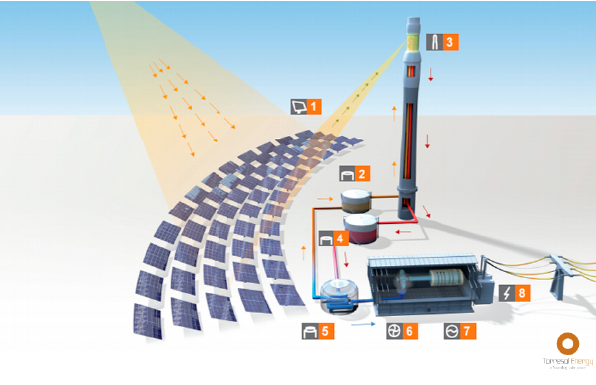
\includegraphics[width=1\linewidth]{Screenshot_15.png}
    \caption{Esquema de una planta termosolar \cite{vivanco2019modelacion}}
    \label{fig:enter-label1}
\end{figure}

A pesar de su potencial, esta tecnología aún se encuentra en desarrollo, especialmente en lo que respecta a los sistemas operativos de plantas termosolares, siendo uno de los principales desafíos la variabilidad de las condiciones climáticas, como el paso de nubes, que impacta directamente en la estabilidad y eficiencia del sistema \cite{marugan2023assessment}. Así, la modelación basada en ecuaciones termodinámicas de la planta contribuiría de manera positiva al problema; sin embargo, esto resulta complejo, costoso y poco práctico, debido a las consideraciones del comportamiento físico real del sistema que se deben tener, como la transferencia de calor, las propiedades térmicas de los materiales, geometrías, flujo del fluido, y las condiciones operativas y de frontera
\cite{mehmood2021simplified}. Por ello, la modelación basada en datos emerge como una alternativa eficaz. Este enfoque permite caracterizar  y comprender el comportamiento de sistemas complejos, evitando la necesidad de modelos paramétricos detallados difíciles de obtener \cite{kalogirou2023solar}. 







\section{Planteamiento del problema}

Los enfoques tradicionales de modelado se basan en la formulación de ecuaciones diferenciales que describen fenómenos como la transferencia de calor y la dinámica de fluidos \cite{10.1145/3514228}. Aplicando leyes físicas fundamentales, estos modelos permiten predecir cómo fluye el calor en un sistema y analizar el efecto de las variables relevantes, como la temperatura, el material o la geometría. Este enfoque facilita entonces la optimización del diseño de sistemas térmicos y su representación simplificada \cite{cengel_transferencia_2013}. En el caso del receptor central en las torres solares, se emplea un enfoque basado en principios de transferencia de calor y dinámica de fluidos, lo que implica utilizar interpolaciones de propiedades térmicas que dependen de variables como la radiación solar incidente, la temperatura y el flujo de aire, integrando además factores climáticos relevantes \cite{ahlbrink2009modeling}. Esto permite describir de manera coherente los procesos involucrados, facilitando una interpretación lógica del comportamiento del modelo y generando resultados consistentes con los esperados \cite{vivanco2019modelacion}. 

Sin embargo, las condiciones transitorias que enfrentan sistemas reales pueden exponer a los modelos a dinámicas complejas y comportamientos no lineales \cite{osorio2022forecasting}. Esto dificulta representar con precisión la diversidad y complejidad del sistema \cite{10.1145/3514228}, teniendo así el desafío de sacar conclusiones y tomar decisiones basadas en información parcial \cite{RAISSI2019686}. Por otro lado, los modelos basados en principios físicos tradicionales son, a menudo, aproximaciones idealizadas, que se basan en un conocimiento incompleto, lo que introduce sesgos y errores en las predicciones \cite{10.1145/3514228}. 

Este proceso de modelado se ve frecuentemente simplificado mediante la adopción de supuestos que, si bien facilitan la formulación del modelo, limitan su capacidad de representar con precisión el comportamiento real del sistema. Entre estos supuestos se encuentran la reducción de detalles microscópicos, como el uso de correlaciones simplificadas de Nusselt y la consideración de propiedades térmicas constantes \cite{ahlbrink2009modeling}; la aplicación de condiciones de frontera idealizadas, como superficies semicirculares con exposición uniforme a la radiación \cite{yang2012numerical}; y la omisión de gradientes térmicos radiales o circunferenciales, lo que puede ocultar sobrecalentamientos localizados en zonas críticas del receptor \cite{Li2025}. Asimismo, se suele despreciar el impacto de los ciclos de arranque y parada, que inducen tensiones térmicas acumulativas en los tubos y se ignoran condiciones operativas transitorias relevantes, como el paso de nubes o la acumulación de suciedad en los heliostatos, factores que alteran significativamente la distribución de flujo térmico sobre el receptor \cite{Li2025, picotti2020object}.

Al no considerar efectos dinámicos y variaciones en las condiciones atmosféricas, el modelo puede subestimar o sobrestimar la cantidad de radiación efectiva en el receptor, influyendo directamente en la estimación de la generación de energía y en las estrategias de control \cite{vivanco2019modelacion}. La omisión de estos efectos dinámicos puede conducir a una sobrestimación de la radiación, lo que llevaría a expectativas de mayor cantidad de energía generada, causando errores en la planificación de la operación real. Mientras que una subestimación puede detectar una menor generación de energía, lo que dificulta alcanzar los objetivos de producción, afectando la economía de la empresa \cite{vivanco2019modelacion}. Un ejemplo representativo es la planta Crescent Dunes, ubicada en Nevada, EE.UU., que utiliza un receptor externo de sales fundidas, la cual enfrentó problemas críticos por sobrecalentamiento en el receptor, atribuible al uso de modelos térmicos simplificados que no consideraron variables dinámicas claves, como las fluctuaciones rápidas en el flujo de calor y los efectos del viento. Estas omisiones contribuyeron a la degradación de los tubos y recubrimientos, lo que derivó en fallas operativas y paradas no planificadas \cite{Li2025}. 

Un enfoque alternativo que también puede ser empleado es la modelación basada en datos. Esta ofrece importantes ventajas para la predicción precisa en condiciones transitorias y con variables operativas fluctuantes \cite{osorio2022forecasting}, especialmente en aquellos sistemas que son inherentemente no lineales y de comportamiento complejo \cite{csurcsia2020user}. A diferencia de los enfoques tradicionales, no requiere la modelización de todos los componentes detalladamente \cite{osorio2022forecasting}, reduce significativamente los costos computacionales y permite construir representaciones efectivas del comportamiento del sistema sin necesidad de un conocimiento a fondo de las leyes físicas que lo rigen \cite{bravo2008modelado}. 

De este modo, la modelación basada en datos presenta varias ventajas clave que la hacen especialmente atractiva para sistemas térmicos complejos. En primer lugar, destaca por su flexibilidad y practicidad, ya que permite representar sistemas cuya descripción mediante ecuaciones físicas sería difícil o costosa, particularmente cuando se enfrentan a alta variabilidad o comportamientos no lineales \cite{bravo2008modelado}. Además, resulta aplicable a sistemas físicos cuya modelación analítica es compleja o inaccesible, pues se basa en datos reales de entrada y salida obtenidos en condiciones operativas reales, evitando la necesidad de conocer en detalle todos los mecanismos internos del sistema \cite{bravo2008modelado}. Otra ventaja importante es que los modelos generados pueden ser utilizados como base para el diseño de estrategias de control y el análisis dinámico del sistema, ofreciendo una representación ajustada a la realidad experimental \cite{Mondal2024}. Finalmente, estos enfoques se caracterizan por su adaptabilidad, ya que pueden ajustarse con rapidez a distintas condiciones de operación, lo que les permite mantener su precisión en entornos cambiantes \cite{Mondal2024}. En conjunto, estos estudios demuestran claramente que la utilización de modelos basados en datos es una estrategia efectiva y aplicable  para gestionar sistemas térmicos complejos y variables, como lo es una planta termosolar de concentración.

A pesar de los importantes avances que ha permitido el modelamiento basado en datos en el contexto de las plantas solares de concentración (CSP), diversos estudios coinciden en que este enfoque presenta aún limitaciones. En el estudio desarrollado por Eid Gul et al. \cite{GUL2025125210}, se advierte que muchos modelos previos se han centrado únicamente en componentes específicos del sistema, sin ofrecer una visión holística que integre el rendimiento técnico, económico y ambiental. Además, la efectividad de estos modelos depende fuertemente de la calidad, cantidad y representatividad de los datos disponibles, lo que puede comprometer su precisión y capacidad de generalización \cite{GUL2025125210}. 



\subsubsection{Brecha identificada}

A partir de las limitaciones identificadas en los modelos tradicionales para describir con precisión el comportamiento no estacionario de sistemas térmicos, sometidos a condiciones variables, se reconoce la necesidad de explorar enfoques alternativos que permitan representar dicha complejidad sin depender exclusivamente de modelos físicos explícitos. Si bien la modelación basada en datos ha mostrado resultados prometedores en diversos campos térmicos, su aplicación específica en sistemas termosolares de concentración sigue siendo escasa. 
Esta falta de desarrollo metodológico y de validación práctica evidencia un vacío que impide avanzar hacia modelos más adaptativos, robustos y útiles en otros escenarios de análisis.
En este contexto, el presente proyecto propone el desarrollo de un modelo computacional no estacionario, basado en datos experimentales, para representar el comportamiento dinámico de un sistema térmico de emulación termosolar a baja escala. El sistema está compuesto por paneles termosolares en los cuales el aporte energético es suministrado mediante resistencias eléctricas, permitiendo reproducir de forma controlada el efecto de la energía térmica que, en un sistema solar real, provendría de la radiación solar incidente.
De esta manera, la investigación busca contribuir al desarrollo metodológico de modelos basados en datos aplicados a sistemas de emulación termosolar, reduciendo la brecha entre los enfoques teóricos existentes y las necesidades prácticas de simulación, análisis y optimización de este tipo de sistemas.


\begin{comment}
Esta es la versión anterior, es demasiado larga

Los enfoques tradicionales de modelado se basan en la formulación de ecuaciones diferenciales que describen fenómenos como la transferencia de calor y la dinámica de fluidos \cite{10.1145/3514228}. Aplicando leyes físicas fundamentales, estos modelos permiten predecir cómo fluye el calor en un sistema y analizar el efecto de las variables relevantes, como la temperatura, el material o la geometría. Este enfoque facilita entonces la optimización del diseño de sistemas térmicos y su representación simplificada \cite{cengel_transferencia_2013}. 

En el caso del receptor central en las torres solares, se emplea un enfoque físico basado en principios de transferencia de calor y dinámica de fluidos, lo que implica utilizar interpolaciones de propiedades térmicas que dependen de variables como la radiación solar incidente, la temperatura y el flujo de aire, integrando además factores climáticos relevantes \cite{ahlbrink2009modeling}. Esto permite describir de manera coherente los procesos involucrados, facilitando una interpretación lógica del comportamiento del modelo y generando resultados consistentes con los esperados \cite{vivanco2019modelacion}. 
Además, cuando las condiciones de frontera y las condiciones iniciales están bien definidas, es posible obtener soluciones analíticas y convergentes, lo cual resulta eficaz en el análisis de fenómenos como la transferencia de calor con fuentes internas, especialmente en contextos lineales y con propiedades del material constantes y controladas \cite{cadena2021applications}. Incluso en sistemas un poco más complejos, como aquellos con fluidos compresibles y conductores de calor en régimen turbulento, las ecuaciones diferenciales permiten construir modelos que capturan adecuadamente este comportamiento físico \cite{kolesnichenko2010thermodynamic}.
En particular, al modelar una planta termosolar bajo estos principios, es posible predecir de manera confiable la evolución de las distribuciones de temperatura, el rendimiento térmico y las respuestas del sistema ante diferentes condiciones operativas, como variaciones en la velocidad del flujo o en la temperatura de entrada del fluido térmico \cite{yang2012numerical}.

Sin embargo, la alta variabilidad presente en muchos sistemas reales y las condiciones transitorias que enfrentan, pueden exponer a los modelos a dinámicas complejas y comportamientos no lineales \cite{osorio2022forecasting} haciendo que existan problemas para captar con precisión esta diversidad y complejidad del sistema \cite{10.1145/3514228}, enfrentando el desafío de sacar conclusiones y tomar decisiones basadas en información parcial \cite{RAISSI2019686}. También, los modelos basados en principios físicos tradicionales son, a menudo, aproximaciones idealizadas, que se basan en un conocimiento incompleto, lo que introduce sesgos y errores en las predicciones \cite{10.1145/3514228}.  
Este proceso de modelización se ve simplificado cuando algunos autores adoptan supuestos como:
\begin{itemize}
    \item Reducción de los detalles microscópicos o fenómenos internos específicos, por ejemplo asumir correlaciones de Nusselt sencillas, ignorar modos de transferencia de calor, o suponer que propiedades como la conductividad térmica y la capacidad calorífica se mantienen constantes \cite{ahlbrink2009modeling}. 
    \item Uso de condiciones de fronteras uniformes y simplificadas, por ejemplo modelar la superficie del tubo como semi-circular expuesta a la radiación y la otra parte aislada \cite{yang2012numerical}
    \item Omitir gradientes radiales o circunferenciales de temperatura, es decir, asumiendo perfiles térmicos uniformes en las secciones transversales de los tubos del receptor, lo que trae como consecuencia una subestimación de las temperaturas máximas en las paredes de los tubos, impidiendo la detección de sobrecalentamientos locales en zonas expuestas a alta irradiancia \cite{Li2025}.
    \item Despreciar el desgaste cíclico del sistema, en una planta termosolar los ciclos de arranque y de parada de la planta son procesos dinámicos, ya que ocurren de forma diaria o en respuesta a la intermitencia climática. Estos cambios operativos generan variaciones térmicas significativas que inducen tensiones en los tubos del receptor, afectando su vida útil a largo plazo \cite{Li2025}.
    \item Ignorar condiciones de operación transitorias comunes, por ejemplo, en una planta solar el paso de nubes genera cambios repentinos en la radiación solar incidente lo que provoca fluctuaciones en la cantidad de energía que estos reflejan hacia el receptor. O también ignorar factores como la acumulación de suciedad en los heliostatos, ya que no ocurre de manera constante en el tiempo. La presencia de polvo o suciedad reduce la eficiencia de reflexión, afectando también la cantidad de radiación dirigida al receptor \cite{picotti2020object}. 
\end{itemize}

Al no considerar efectos dinámicos y variaciones en las condiciones atmosféricas, el modelo puede subestimar o sobrestimar la cantidad de radiación efectiva en el receptor, lo que influye directamente en la estimación de la generación de energía y en las estrategias de control \cite{vivanco2019modelacion}. La omisión de estos efectos dinámicos puede conducir a que una sobrestimación de la radiación puede llevar a expectativas de mayor cantidad de energía generada, causando errores en la planificación de la operación real. Mientras que una subestimación puede detectar una menor generación de energía, lo que dificulta alcanzar los objetivos de producción, afectando la economía de la empresa \cite{vivanco2019modelacion}. Un ejemplo representativo es la planta Crescent Dunes, ubicada en Nevada, EE.UU., que utiliza un receptor externo de sales fundidas, la cual enfrentó problemas críticos por sobrecalentamiento en el receptor, atribuible al uso de modelos térmicos simplificados que no consideraron variables dinámicas clave, como las fluctuaciones rápidas en el flujo de calor y los efector del viento. Estas omisiones contribuyeron a la degradación de los tubos y recubrimientos, lo que derivó en fallas operativas y paradas no planificadas \cite{Li2025}. 

Otro enfoque que también puede ser empleado es la modelación basada en datos. Esta ofrece importantes ventajas para la predicción precisa en condiciones transitorias y con variables operativas fluctuantes \cite{osorio2022forecasting}, especialmente en aquellos sistemas que son inherentemente no lineales y de comportamiento complejo \cite{csurcsia2020user}. A diferencia de los enfoques tradicionales, no requiere la modelización de todos los componentes detalladamente \cite{osorio2022forecasting}, reduce significativamente los costos computaciones y permite construir representaciones efectivas del comportamiento del sistema sin necesidad de un conocimiento a fondo las leyes físicas que lo rigen \cite{bravo2008modelado}. 
De este modo, la modelización basada en datos ofrece varias ventajas clave:
\begin{itemize}
\item \textbf{Opcionalidad y practicidad:} Facilita la representación de sistemas complejos o desconocidos, cuya descripción mediante leyes físicas y ecuaciones diferenciales sería difícil o costosa, especialmente en casos con alta variabilidad o dinámicas no lineales \cite{bravo2008modelado}. 
\item \textbf{Aplicabilidad a sistemas físicos difíciles de modelar:} Útil en la determinación de modelos cuya caracterización analítica es compleja, los cuales requieren una solución basada en mediciones de entrada y salida obtenidas en condiciones reales de operación \cite{bravo2008modelado}.
\item \textbf{Base para control y análisis:} Los modelos obtenidos pueden ser usados posteriormente en el diseño de estrategias de control y en el análisis del comportamiento dinámico del sistema, con una fidelidad ajustada a los datos experimentales \cite{Mondal2024}.
\item \textbf{Adaptabilidad:} La utilización de datos permite al sistema adaptarse ágilmente a diferentes condiciones operativas \cite{Mondal2024}.
\end{itemize}

Dentro del campo de la ingeniería existen estudios asociados al modelamiento de procesos basado en datos, por ejemplo, el desarrollado por Karthik Duraisamy, Gianluca Iaccarino y Heng Xiao \cite{duraisamy2019turbulence} el cual demostró que esta metodología mejora significativamente la capacidad predictiva de los modelos de turbulencia en mecánica de fluidos, especialmente aquellos basados en RANS (Reynolds-Averaged Navier–Stokes), una técnica ampliamente utilizada para representar flujos turbulentos. Los autores lograron cuantificar y reducir la incertidumbre asociada a parámetros y tensores de Reynolds, mejorando la precisión en la estimación de variables clave como la velocidad del flujo y el esfuerzo cortante. Además, desarrollaron funciones de corrección que pueden generalizarse a distintos tipos de flujo, aseguraron la coherencia física de los modelos mediante la integración de restricciones matemáticas y principios conocidos de la dinámica de fluidos. Esto permitió construir modelos más robustos, con capacidad adaptativa a diferentes escenarios y con predicciones acompañadas de estimaciones explícitas de incertidumbre \cite{duraisamy2019turbulence}.
Otro artículo, realizado por Shashikant Ilager, Kotagiri Ramamohanarao y Rajkumar Buyya \cite{ilager2020thermal}, aplicó modelado basado en datos para predecir la temperatura en servidores de centros de datos. Mediante técnicas de aprendizaje automático, desarrollaron un modelo capaz de anticipar el comportamiento térmico de los servidores utilizando únicamente datos de sensores físicos. Su enfoque logró un error medio de predicción de solo 2.38\%, permitió reducir la temperatura máxima en 6.5°C y disminuyó el consumo energético en un 34.5\%, abordando así uno de los principales retos operacionales: el alto consumo energético asociado a la refrigeración, que puede representar hasta el 50\% del uso total de energía en estos sistemas \cite{ilager2020thermal}.
En el campo específico de las plantas termosolares, también se han desarrollado enfoques basados en datos con resultados importantes. Por ejemplo, un estudio reciente implementó técnicas de inteligencia artificial para calibrar el enfoque de heliostatos en plantas solares de torre. El modelo fue entrenado con datos reales de operación y alcanzó una precisión cercana al 89 \% en la predicción de la orientación óptima de los espejos \cite{KUHL2024112894}.
Asimismo, el trabajo de Mondal et al. \cite{Mondal2024} emplea esta metodología para predecir de manera eficaz el rendimiento de plantas térmicas, enfocándose en variables clave como la eficiencia térmica, el consumo específico de combustible y la generación de potencia. Esta capacidad predictiva permitió optimizar la operación de la planta en tiempo real, mejorando la toma de decisiones operativas y reduciendo el impacto de las fluctuaciones dinámicas \cite{Mondal2024}. 
Particularmente relevante para las plantas termosolares de concentración es el estudio realizado por Jianxing Wang, Lili Guo, Chengying Zhang, Lei Song, Jiangyong Duan y Liqiang Duan \cite{Wang2020}, el que evidenció que estas técnicas permiten capturar con precisión las complejas relaciones no lineales y patrones espacio-temporal entre variables meteorológicas y potencia térmica. Al integrarse con modelos físicos, mejoran la precisión de las predicciones y reducen la subjetividad en la selección de variables, lo cual es crucial para un operación segura, eficiente y económicamente viable de los sistemas solares de torre \cite{Wang2020}.


En conjunto, estos estudios demuestran claramente que la utilización de modelos basados en datos es una estrategia efectiva y aplicable  para gestionar sistemas térmicos complejos y variables, como lo es una planta termosolar de concentración.

A pesar de los importantes avances que ha permitido el modelamiento basado en datos en el contexto de las plantas solares de concentración (CSP), diversos estudios coinciden en que este enfoque presenta aún limitaciones. En el estudio desarrollado por Eid Gul y colaboradores \cite{GUL2025125210}, se advierte que muchos modelos previos se han centrado únicamente en componentes específicos del sistema, sin ofrecer un visión holística que integre el rendimiento técnico, económico y ambiental. Además, la efectividad de estos modelos depende fuertemente de la calidad, cantidad y representatividad de los datos disponibles, lo que puede comprometer su precisión y capacidad de generalización \cite{GUL2025125210}. Por otro lado, el estudio de Yaseen y Alawi, sobre modelos de inteligencia artificial para predecir el factor de rentabilidad en sistemas CSP con respaldo dual \cite{yaseen2025artificial}, identifica como un desafío adicional la alta estocasticidad y no linealidad de los parámetros de entrada, lo que complica el desarrollo de modelos computaciones simples y estables para sistemas tan complejos, como una planta CSP \cite{yaseen2025artificial}. Se destaca también que algunos modelos de inteligencia artificial sofisticados, aunque aumentan la precisión, necesitan un tiempo de entrenamiento más largo e implican un mayor riesgo de sobreajuste \cite{yaseen2025artificial}. De igual manera, la flexibilidad operativa de un modelo de redes neuronales está limitada a las variaciones dentro del conjunto de entrenamiento, es decir, cualquier cambio en la geometría del receptor, en las propiedades térmicas del fluido o condiciones operativas  atípicas requiere reentrenar la red neuronal desde cero \cite{tuman2025neural}. 

 A partir de las limitaciones identificadas en los modelos tradicionales para describir con precisión el comportamiento no estacionario de sistemas térmicos, sometidos a condiciones reales y transitorias, donde la complejidad del sistema, las múltiples interacciones físicas y las fuertes no linealidades que podría presentar, obligan a realizar simplificaciones que introducen errores significativos, a requerir un conocimiento más profundo del sistema y a aumentar el costo computacional, surge la necesidad de desarrollar enfoques alternativos. En este sentido, la modelización basada en datos emerge como una poderosa herramienta, capaz de capturar comportamientos complejos sin depender estrictamente de representaciones físicas explícitas. Además, permite la adaptación a datos experimentales reales y reducir la necesidad de suposiciones idealizadas.
Considerando también los estudios que avalan la utilización de este enfoque en sistemas térmicos, el presente proyecto propone el desarrollo de un modelo computacional no estacionario, basado en datos experimentales, que permita representar de manera precisa el comportamiento dinámico de un sistema termosolar a baja escala. A futuro, esta herramienta podrá ser escalada y aplicada al análisis y optimización de plantas termosolares reales, facilitando el diseño de estrategias de control y la validación de modelos predictivos.
\end{comment}
\section{Organización del documento}
El presente documento corresponde al desarrollo de una tesis de magíster cuyo objetivo es identificar y validar un modelo basado en datos para representar el comportamiento dinámico de un sistema térmico de emulación termosolar a baja escala.

El Capítulo 1 presenta la contextualización general de la investigación y define el problema que se busca abordar. En este capítulo se exponen el planteamiento del problema, el objetivo general y los objetivos específicos, junto con la justificación del estudio, destacando su relevancia tanto desde una perspectiva teórica como aplicada.

El Capítulo 2 describe  la metodología utilizada para el desarrollo de los objetivos específicos planteados. 

El Capítulo 3 presenta una revisión del estado del arte. En esta sección se analizan los principales enfoques de modelado utilizados para representar sistemas térmicos, con énfasis en las estructuras lineales y no lineales basadas en datos. Además, se revisan las características de las señales de excitación empleadas en identificación de sistemas y su pertinencia para el banco de ensayos estudiado.

El Capítulo 4 desarrolla la caracterización experimental del sistema mediante el diseño y la aplicación de señales de excitación. Asimismo, se describe el proceso de identificación de los distintos modelos evaluados y se presentan sus resultados de validación, tanto en el dominio temporal como en el dominio frecuencial.

Finalmente, el Capítulo 5 reúne las principales conclusiones obtenidas a partir del trabajo realizado y presenta las líneas de investigación futura que surgen de los resultados, limitaciones y oportunidades de mejora identificadas durante el desarrollo de la tesis.
    

\section{Objetivos}

\subsection{Objetivo general}
Desarrollar un modelo computacional, basado en datos experimentales, que represente el comportamiento no estacionario de un sistema de emulación termosolar a baja escala.
%de un sistema térmico de baja temperatura
%de un sistema de calentamiento a baja temperatura
%de un sistema térmico de baja escala

\subsection{Objetivos específicos}

\begin{itemize}
\item Revisar en el estado del arte los enfoques existentes de modelado dinámico de sistemas térmicos basados en datos experimentales.
\item Caracterizar el comportamiento dinámico del sistema mediante experimentación bajo diferentes condiciones de operación.
%\item Caracterizar el comportamiento dinámico del sistema mediante experimentación, identificando sus no linealidades bajo diferentes condiciones de operación.
\item Desarrollar el modelo computacional basado en datos de acuerdo con la caracterización realizada al sistema.
\item Validar el modelo bajo las condiciones normales de operación del sistema. 
\end{itemize}

\section{Alcance}

El presente trabajo se centra en el desarrollo de un modelo computacional no estacionario, basado en datos experimentales, que represente el comportamiento térmico dinámico de un sistema de emulación termosolar a escala reducida. El modelo se construyó a partir de registros obtenidos en ensayos experimentales controlados, considerando variables como temperatura, caudal y aporte de energía térmica, con el objetivo de capturar la respuesta real del sistema bajo condiciones operativas variables. 
El estudio contempla la revisión de metodologías de modelado basadas en datos, la identificación de características dinámicas y no lineales del sistema y la selección de la técnica de modelado más adecuada. Asimismo, se incluye la validación del modelo en simulación libre, evaluando su capacidad para reproducir la evolución temporal del sistema. Cabe señalar que este proyecto no abarca el diseño ni la implementación de estrategias de control basadas en el modelo desarrollado. No obstante, se espera que el modelo generado pueda servir como base para futuros trabajos orientados al control de sistemas térmicos.

El sistema experimental utilizado se encuentra instalado en un laboratorio de la Facultad de Ciencias de la Ingeniería de la Universidad Austral de Chile y está conformado por colectores solares de placa plana, válvulas de control de flujo, medidores de caudal, sensores de temperatura y resistencias eléctricas encargadas de suministrar calor al fluido térmico. Esta configuración permite desarrollar ensayos bajo condiciones controladas y reproducibles, ya que el aporte energético es proporcionado mediante la red eléctrica, reduciendo la dependencia de variables externas como las condiciones climáticas o interrupciones propias de una operación en ambiente exterior.
El conjunto experimental tiene como propósito emular, a baja escala, ciertos aspectos dinámicos de un sistema termosolar de concentración, particularmente aquellos asociados al transporte de energía térmica mediante un fluido en circulación. En este sentido, el recorrido del fluido a través de los colectores permite reproducir fenómenos relevantes como la transferencia de calor, el acoplamiento térmico entre componentes, los retardos de transporte y la acumulación energética.
Sin embargo, presenta diferencias importantes respecto de una instalación termosolar real. Entre ellas, destaca que el calor no proviene de radiación solar concentrada, por lo que no se reproduce una variabilidad espacial de la irradiancia sobre el sistema. Además, las condiciones de temperatura, potencia, escala, pérdida térmica e interacción con el ambiente son propias de un montaje de laboratorio, por lo que difieren de las observadas en una planta real.
Por lo tanto, el sistema no debe entenderse como una réplica completa de una planta termosolar de concentración, sino como una plataforma experimental controlada que permite estudiar la dinámica térmica de un sistema con circulación de fluido y aporte energético regulable. En este contexto, su principal utilidad radica en la obtención de datos experimentales para el desarrollo y validación de modelos computacionales basados en datos.

Adicionalmente, durante el desarrollo del trabajo se presentaron diversas limitaciones experimentales y computacionales que condicionaron la ejecución de los ensayos y el proceso de identificación de los modelos. Entre las limitaciones experimentales se encontró la falla de una de las resistencias eléctricas del banco de ensayos, la cual debió ser reemplazada, así como la falla de un sensor de nivel que provocó una descarga inesperada de agua desde el estanque de almacenamiento hacia el laboratorio. Asimismo, la capacidad y estabilidad de la instalación eléctrica del laboratorio constituyeron una restricción relevante, debido a que la operación simultánea de otras herramientas o equipos eléctricos produjo cortes de energía. Estas interrupciones modificaron las condiciones de operación del sistema y provocaron la pérdida de registros experimentales, haciendo necesario repetir determinados ensayos y generando retrasos en el desarrollo del estudio.

Por otra parte, el proceso de identificación presentó limitaciones asociadas al costo computacional requerido para explorar distintas estructuras, órdenes, retardos y combinaciones de parámetros de los modelos analizados. En particular, el aumento del número de coeficientes y regresores incrementa considerablemente el espacio de búsqueda y el tiempo necesario para el ajuste y validación de cada estructura. Debido a estas restricciones, no fue posible realizar una exploración de todas las configuraciones potencialmente disponibles. En consecuencia, los modelos seleccionados corresponden a las mejores estructuras identificadas dentro del espacio de búsqueda evaluado en este trabajo. Una exploración más amplia de la complejidad estructural podría ser abordada en investigaciones futuras, considerando además el compromiso entre capacidad de representación, costo computacional y riesgo de sobreajuste.  



\begin{comment}
Versión anterior

Este trabajo se centra en el desarrollo de un modelo computacional no estacionario, basado en datos experimentales, que represente el comportamiento térmico de un sistema termosolar a pequeña escala. El modelo se construye a partir de registros obtenidos mediante ensayos, con el objetivo de capturar las características reales del sistema, como la recolección de datos de temperatura, caudal y energía. El estudio incluye la revisión y análisis de metodologías basadas en datos, así como la identificación de las características dinámicas y no lineales del sistema. Con esto se realizará la selección y formulación de la técnica más adecuada de modelo computacional  para representar al sistema. También se considera la validación del modelo en condiciones normales de operación, evaluando su capacidad de replicar el comportamiento real del sistema. Este modelo está concebido como una herramienta base que podría ser utilizada como punto de partida para el desarrollo de estrategias de control de un sistema térmico. El estudio y desarrollo de dichas estrategias se encuentra fuera del alcance del presente proyecto.

El sistema experimental utilizado para este proyecto se encuentra ubicado en un laboratorio de la facultad y está conformado por colectores solares de placa plana, válvulas de control de flujo, medidores de caudal, sensores de temperatura y resistencias eléctricas, las cuales tienen la función de suministrar calor al fluido. Aquí es donde se identifica una primer limitante, ya que la fuente de energía térmica no es solar, sino eléctrica, por lo que los transientes en la radiación solar pueden no ser totalmente reproducibles, aunque las temperaturas siguen siendo medidas a la salida de cada panel, por lo que dicho punto refleja la realidad de un sistema expuesto a la radiación solar. No obstante, el punto a favor es que se tiene una dependencia directa de la red eléctrica local, y si esta no falla, el sistema se puede estudiar con más detalle en condiciones más estables. Un inconveniente relevante está asociado a la integridad física del sistema: una falla en alguno de los sensores podría afectar significativamente la recolección de datos y provocar retrasos en el desarrollo del proyecto. Asimismo, se prevén limitaciones de carácter computacional, dado el gran volumen de datos que se espera recopilar durante los experimentos, requiriendo una capacidad de procesamiento y almacenamiento significativa para su análisis y modelado.
\end{comment}

\section{Justificación}

En la actual transición energética, las plantas termosolares han tomado protagonismo como una fuente limpia y eficiente de generación de energía. Este creciente interés ha impulsado su estudio y ha puesto de manifiesto uno de sus principales desafíos: la modelación precisa del comportamiento térmico no estacionario que presentan estos sistemas, especialmente cuando operan bajo condiciones reales y variables. Los modelos físicos tradicionales, aunque útiles, suelen requerir simplificaciones que reducen su capacidad predictiva y aumentan la complejidad computacional, dificultando su implementación práctica en tiempo real. 

Frente a estas limitaciones, el presente proyecto propone un enfoque alternativo basado en datos experimentales para el desarrollo de un modelo computacional no estacionario que represente el comportamiento térmico de un sistema termosolar a baja escala. Este enfoque permite capturar las dinámicas transitorias del sistema y sus no linealidades directamente desde su respuesta empírica, sin necesidad de formular modelos físicos complejos. Se espera que esta estrategia no solo reduzca la carga computacional, sino que ofrezca una herramienta más flexible para su uso posterior en análisis, simulación o control.

La utilización de un sistema experimental de laboratorio permite validar el modelo en un entorno controlado, reproduciendo distintas condiciones operativas que reflejan los desafíos reales en el funcionamiento de plantas CSP. La generación y el análisis de datos en este entorno no solo fortalece la comprensión del sistema, sino que también abre las posibilidades de transferir el enfoque propuesto a escalas mayores o a diferentes tipos de instalaciones. Asimismo, este modelo podría ser empleado como base para el diseño e implementación de estrategias de control más eficientes y adaptativas. 

Por lo tanto, este trabajo contribuye al avance del modelado de sistemas térmicos mediante técnicas basadas en datos, integrando experimentación y análisis computacional con el fin de desarrollar herramientas más flexibles, eficientes y adaptables para el desarrollo de tecnologías termosolares.


\chapter{Metodología}

Para alcanzar los objetivos propuestos, se sigue una metodología estructurada en cuatro etapas principales, alineadas con cada uno de los objetivos específicos.
\begin{enumerate}

\item \textbf{Revisión del estado del arte de los enfoques existentes de modelado dinámico de sistemas térmicos basados en datos experimentales.}

En la etapa inicial, se realizó una revisión bibliográfica de trabajos, artículos y documentación científica relevante sobre el modelado dinámico de sistemas térmicos a partir de datos experimentales. La búsqueda se hizo refinando y ajustando las palabras clave a medida que se analizaron los resultados, con el fin de mejorar la relevancia y precisión de la información. Esta revisión permitió identificar los enfoques más utilizados, contextos de aplicación, herramientas utilizadas y niveles de complejidad. 
La búsqueda se enfocó en diversos aspectos específicos de cada estudio, tales como:
\begin{itemize}

\item Tipos de modelos y metodologías existentes, como lineales, no lineales, basados en datos y modelos híbridos.
\item Clasificación de los modelos basados en datos existentes, destacando sus ventajas, limitaciones y condiciones óptimas de uso.
\item La naturaleza y características de los datos utilizados.
\item El tipo de señales de entrada aplicadas en los experimentos, con el propósito de compararlas y seleccionar posteriormente las más adecuadas para el sistema que se va a modelar.
\end{itemize}
Además, se buscó identificar si los estudios presentan enfoques o criterios para detectar no linealidades en los sistemas térmicos, ya sea mediante análisis espectral, curvas de respuesta, indicadores estadísticos, entre otros. Estas herramientas se consideraron para etapas posteriores del trabajo.
Como resultado de esta revisión, se construyó  una base de conocimiento estructurada mediante tablas comparativas que indicaron:
\begin{itemize}
    \item   Los tipos de modelos basados en datos, junto a su aplicación típica, ventajas, limitaciones y complejidad.
\item Los tipos de señales adecuadas para excitar el sistema, la cobertura espectral de cada una, el factor de cresta, aplicación típica y facilidad de implementación.
\end{itemize}
Esto, además de facilitar la comparación entre los enfoques encontrados, sirvió como base para tomar decisiones informadas en el desarrollo posterior del trabajo.


\item \textbf{Caracterización del comportamiento dinámico del sistema mediante experimentación bajo diferentes condiciones de operación.}

A partir del conocimiento adquirido en la etapa anterior, se diseñaron e implementaron experimentos destinados a excitar adecuadamente al sistema térmico en estudio, con el propósito de observar y registrar el comportamiento no estacionario del banco de ensayo bajo diferentes condiciones.
Para ello se definieron las señales de entrada adecuadas, que permiten una excitación apropiada para detectar la dinámica relevante del sistema. Durante la ejecución de los experimentos, se realizó un registro detallado de todas las variables que entregan los sensores del banco, asegurando una alta resolución temporal y una cobertura suficiente de las condiciones de operación.
Es importante considerar que, si bien las pruebas se desarrollaron en un entorno controlado de laboratorio, existen variables externas, como la temperatura ambiente y la temperatura de entrada del agua, que no pueden ser controladas completamente. Por lo tanto, estos valores se registraron como referencia para evaluar su posible influencia sobre la respuesta del sistema.

El análisis de datos experimentales permitió identificar cómo reacciona el sistema frente a diferentes perturbaciones y condiciones de entrada. Este análisis permitió caracterizar el sistema y visualizar su respuesta mediante gráficos, espectros de frecuencia y curvas entrada–salida, evidenciando su comportamiento dinámico.

El resultado de esta etapa fue la caracterización no estacionaria del sistema, describiendo cómo responde frente a distintas señales de excitación. 



\item \textbf{Desarrollo del modelo computacional basado en datos de acuerdo con la caracterización realizada al sistema.}

Con base en los datos experimentales recopilados y la caracterización dinámica del sistema, se procedió al desarrollo de modelos computacionales. La estructura del modelo más adecuada se seleccionó considerando la caracterización identificada durante la etapa experimental.
Inicialmente se evaluaron estructuras lineales SISO, considerando el caudal como entrada y la temperatura como salida. Se identificaron modelos ARX, Output-Error y Box-Jenkins. Posteriormente, al incorporar la potencia de las resistencias eléctricas como segunda entrada, se desarrolló una estructura MISO lineal Box-Jenkins y se evaluaron dos estructuras no lineales: un modelo NARX y un modelo basado en una red neuronal con ecuaciones diferenciales ordinarias.

Respecto del entorno computacional, se utilizaron herramientas de software libre debido a las limitaciones del proyecto. Por esta razón, Python fue seleccionado como entorno principal por su flexibilidad, amplia disponibilidad de bibliotecas científicas y de aprendizaje automático, su facilidad de integración con bases de datos y su creciente uso en el ámbito académico e industrial. Aunque existen otras opciones de código abierto como R, Julia o GNU Octave, Python ofrece un equilibrio entre capacidades numéricas, documentación y facilidad de uso.

\item \textbf{Validación del modelo bajo las condiciones normales de operación del sistema.}

Para finalizar, los modelos desarrollados fueron validados mediante datos independientes del conjunto de datos de identificación. Esta etapa fue fundamental para evaluar la capacidad predictiva de los modelos, su robustez ante posibles variaciones externas y su utilidad práctica para futuras aplicaciones.
La validación se llevó a cabo mediante la comparación entre las salidas del modelo y los datos reales del sistema. Para cuantificar el desempeño del modelo, se calcularon diversas métricas de evaluación, entre las cuales se consideran:
\begin{itemize}
     \item Coeficiente de determinación ($R^2$): Indica qué proporción de la variabilidad presente en los datos puede ser explicada por los valores estimados. Un valor cercano a 1 representa una alta capacidad explicativa, mientras que un valor cercano a 0 indica una capacidad explicativa limitada. Por su parte, valores negativos muestran un desempeño inferior al que se obtendría utilizando el valor medio de los datos observados como referencia. Se calcula como:
 \begin{equation} \label{coef de determinación}
        R^2 = 1 - \frac{\sum_{i=1}^{n} (y_i - \hat{y}_i)^2}{\sum_{i=1}^{n} (y_i - \bar{y}_i)^2}
\end{equation}
        donde:
        \begin{itemize}
            \item $y_i$: Salida medida.
            \item $\hat{y_i}$: Salida estimada.
            \item $\bar{y}$: Promedio de salida medida.
            \item $n$: Número de muestras.
        \end{itemize}
   
    \item Raíz del Error Cuadrático Medio (RMSE): Evalúa la precisión predictiva del modelo mediante la cuantificación de la magnitud promedio del error entre los valores predichos y los valores reales del sistema \cite{10.3389/fenrg.2022.822555}. Su expresión es:
 \begin{equation} \label{rmse} 
        RMSE=\sqrt{\frac{1}{n}\sum_{i=1}^{n}{(y_i-\hat{y_i})^2}}
       \end{equation} 
    
    \item Error Absoluto Medio (MAE): Representa el promedio del valor absoluto de las diferencias entre la salida medida y la salida estimada. A diferencia del RMSE, esta métrica entrega una medida más directa del error promedio, sin penalizar de forma cuadrática las desviaciones mayores. Se calcula como\cite{ALQATAMIN2025128344}:
\begin{equation} \label{mae} 
        MAE=\frac{\sum_{i=1}^{n}{|y_i-\hat{y_i}|}}{n}
\end{equation}
    \item FIT: Corresponde a una métrica utilizada en identificación de sistemas que representa el porcentaje de ajuste entre la respuesta del modelo y la señal medida, evaluando cuánto del comportamiento dinámico de la salida es reproducido por el modelo en comparación con la variabilidad total de los datos experimentales. Valores cercanos al 100\% indican una alta concordancia entre la salida simulada y la salida real, mientras que valores bajos reflejan una menor capacidad de representación dinámica \cite{ljung1999system} \cite{MUSTAFARAJ2010348}. Se define como:
\begin{equation} \label{fit} 
         FIT=100 (1- \frac{\sqrt{\sum_{i=1}^{n}{(y -\hat{y})^2}}}{\sqrt{\sum_{i=1}^{n}{(y- \bar{y})^2}}})
\end{equation}


   
\end{itemize}
Además de estas métricas numéricas, se incluyen gráficos de validación como comparaciones visuales entre la salida simulada y la medida, análisis de residuos para detectar patrones sistemáticos no modelados o evaluación temporal del error en distintas condiciones. Asimismo, se utilizaron indicadores frecuenciales como la función de respuesta en frecuencia (FRF), la coherencia y la densidad espectral para comparar la salida simulada con la salida real.


\end{enumerate}




\chapter{Revisión del estado del arte} 

En esta sección se presenta una revisión de las principales metodologías de modelado basadas en datos experimentales aplicadas a sistemas térmicos dinámicos, con énfasis en aquellos sistemas que presentan variaciones temporales, retardos, acoplamiento entre variables de entrada y salida y posibles comportamientos no lineales. Este análisis resulta relevante para el sistema de emulación termosolar en estudio, ya que su dinámica térmica depende de variables operacionales como el caudal y la potencia térmica suministrada, las cuales influyen directamente en la evolución temporal de la temperatura del fluido. En consecuencia, la selección de una estructura de modelo adecuada requiere estudiar previamente las características dinámicas del sistema, tales como su linealidad o no linealidad, los retardos dominantes, la respuesta frecuencial y la sensibilidad frente a distintas señales de excitación.
Asimismo, se revisan criterios asociados al diseño de experimentos para identificación de sistemas, particularmente en relación con la selección de señales de entrada suficientemente informativas. En sistemas térmicos, donde las respuestas suelen ser lentas y estar influenciadas por fenómenos como la acumulación térmica y la transferencia de calor, la calidad de los datos experimentales es determinante para obtener modelos representativos. Por esta razón, se consideran aspectos como la persistencia de excitación, la independencia entre entradas, el contenido frecuencial de las señales y la relación entre las variables manipuladas y la salida térmica \cite{csurcsia2020user}.


La modelación basada en datos se centra en el análisis de registros experimentales sin asumir una estructura definida del sistema. De forma general, el proceso de identificación considera la selección de señales de excitación adecuadas, el preprocesamiento de los datos, la verificación de la independencia entre canales de entrada, el análisis frecuencial de las variables medidas y la posterior construcción y validación del modelo \cite{csurcsia2020user}. Estos aspectos son especialmente importantes en sistemas de energía térmica que operan bajo condiciones dinámicas y variables, como los sistemas solares con almacenamiento térmico, los cuales pueden presentar comportamientos inherentemente no lineales que dificultan su modelación precisa \cite{osorio2022forecasting}. Esta complejidad se ve acentuada por la falta de herramientas universales capaces de representar adecuadamente todos los escenarios posibles de dichos sistemas \cite{csurcsia2020user}.



No obstante, diversos enfoques de modelado han demostrado ser útiles para aproximar el comportamiento de sistemas no lineales, particularmente cuando se requiere formular estrategias de control. En este contexto, los modelos dinámicos resultan fundamentales, ya que permiten estimar el comportamiento futuro del sistema, lo que a su vez posibilita determinar acciones de control eficaces. Además, estos modelos facilitan la incorporación explícita de restricciones del proceso, aspecto relevante en la regulación de sistemas complejos o con limitaciones operativas estrictas \cite{Schwenzer2021mpc}. Por ejemplo, en sistemas de climatización de edificios, el modelado dinámico permite simular con precisión los cambios de temperatura y humedad en el ambiente, contribuyendo a mejorar la eficiencia energética y el confort térmico de los usuarios \cite{LI2025135822}. Es esencial, por lo tanto, para captar comportamientos temporales y fluctuaciones en la temperatura, siendo fundamentales para la implementación efectiva de sistemas de control predictivo \cite{Fick2025}. 
Un modelado preciso de la dinámica del sistema es indispensable para el diseño de estrategias de control robustas y adaptativas, capaces de anticipar y responder a incertidumbres, perturbaciones y variaciones operacionales \cite{Lv2025RMPCDeepLearning}. En este sentido, las técnicas de modelado asistido por datos aplicadas a sistemas dinámicos permiten mejorar significativamente la representación y adaptabilidad de los sistemas térmicos \cite{zhou2024review}. Por ejemplo, en turbinas de gas, se ha utilizado regresión lineal para estimar variables clave como temperatura y potencia. Asimismo, las redes neuronales tipo NARX se han empleado para modelar componentes como válvulas, compresores y turbinas bajo condiciones de arranque o carga variable. Estas herramientas permiten identificar parámetros o construir relaciones funcionales entre variables de entrada y salida, lo que mejora la adaptación del modelo frente a degradaciones, perturbaciones o cambios en la demanda operativa \cite{zhou2024review}.
%Un modelado preciso de la dinámica del sistema es indispensable para diseñar controles robustos y adaptativos, como el RMPC (Robust Model Predictive Control) y Deep Learning (técnicas de aprendizaje autónomo basadas en redes neuronales profundas), que puedan anticipar y responder eficazmente a las incertidumbres y variaciones en las condiciones de operación\cite{Lv2025RMPCDeepLearning}.





%En el entorno de operación de sistemas reales en condiciones muy precisas, las simulaciones rápidas y confiables son cruciales. En el caso de sistemas térmicos se usan algunos modelos basados en datos como los sistemas lineales invariantes en el tiempo (LTI), que describen la evolución temporal de la temperatura del fluido en elementos como las tuberías. Para ello se necesitan datos confiables que permitan desarrollar un modelo de orden reducido (ROM, en inglés). Este se obtiene de la reducción de la ley de conservación de la energía para cada elemento discreto mediante una relación de entrada-salida semianalítica entre las temperaturas involucradas. Los datos de entrenamiento se generan mediante modelos computacionales basados en la física, a través de experimentos de calibración o en mediciones de campo. Este modelo se basa en el balance de energía discretizado en 3D, capturando todo el comportamiento físico y la dinámica exhibida del sistema. Esto permite predecir el comportamiento futuro fuera del rango de los datos de entrenamiento y requerir un conjunto de datos no tan denso para su calibración. El modelo reduce significativamente el costo computacional en comparación con modelos FOM (Modelos de Orden Completo basados en la física), siendo dependiente directamente del numero de pasos de tiempo, mientras que el del FOM depende de la resolución espacial y temporal \cite{JIANG2023121038}. 



La aplicación de redes neuronales de memoria a largo y corto plazo, conocidas como LSTM (\textit{Long Short-Term Memory}), integradas con principios físicos, también ha permitido desarrollar modelos dinámicos basados en datos, capaces de capturar eficazmente las dependencias temporales en sistemas de intercambio de calor \cite{TANG2025127322}.  En este tipo de aplicaciones, se han utilizado como variables de entrada la temperatura y caudales másicos, junto con procedimientos de filtrado orientados a mitigar los efectos del ruido y mejorar la calidad de los datos. Las salidas consideradas corresponden, por ejemplo, a la temperatura de salida del intercambiador. Además, estos modelos pueden incorporar variables físicas relevantes, como la temperatura del fluido caliente y del fluido frío, la temperatura de la pared, los caudales másicos de ambos lados del intercambiador, la tasa de transferencia de calor, la capacidad térmica específica del fluido, área y coeficientes de transferencia de calor, capacidad calorífica, resistencia térmica, así como variables asociadas al tiempo y presión de operación \cite{TANG2025127322}.

En función de lo anterior, la revisión del estado del arte se orienta a analizar las principales alternativas de modelado dinámico basadas en datos empleadas en sistemas térmicos. Esta revisión permite establecer los criterios necesarios para seleccionar una estructura de modelo adecuada al sistema estudiado. De igual manera, se abordan aspectos relacionados con el diseño de señales de excitación necesarias para obtener datos suficientemente informativos. De esta forma, los apartados siguientes presentan los fundamentos y aplicaciones de distintas técnicas de modelado basado en datos, con el propósito de justificar la metodología empleada posteriormente en el trabajo.

\begin{comment}
Lo que estaba aquí lo moví al inicio

El modelamiento basado en datos se centra en el uso de técnicas no paramétricas, las cuales permiten observar directamente los datos sin asumir una estructura funcional específica del sistema. Estas técnicas, apoyadas en métodos estadísticos, facilitan la estimación de funciones de respuesta en frecuencia (FRF), la identificación de no linealidades y la detección de fallas o problemas en las mediciones. Todo esto sin recurrir a un modelo paramétrico predefinido. El proceso general incluye:
\begin{itemize}
    \item Diseño del experimento: Se seleccionan excitaciones multisinusoidales apropiadas para estimular el sistema, asegurando que los canales de entrada sean independientes y que la señal sea adecuada para distinguir comportamientos lineales y no lineales
    \item Preprocesamiento de datos: Consiste en la eliminación de tendencias, segmentación de datos en períodos y realizaciones, y verificación de la independencia de las señales de entrada (control de correlación).
    \item Estimación de respuesta en frecuencia y análisis estadístico: Se calcula la FRF y se utiliza la función de coherencia y otras estadísticas avanzadas para detectar no linealidades y ruido, permitiendo así comprender mejor la naturaleza del sistema.
    \item Evaluación de no linealidades y calidad de medición: A través de análisis de la coherencia, la estimación de no linealidades y otros indicadores, se decide si el modelo lineal es suficiente o si se requiere un modelo más avanzado.
    \item Modelamiento y toma de decisiones: La información obtenida se usa para construir modelos no paramétricos o paramétricos, determinando si la simplificación lineal es adecuada o si se recomienda un enfoque no lineal, además de valorar cuánto se gana usando modelos más complejos \cite{csurcsia2020user}.
\end{itemize}
\end{comment} 

\begin{comment}  
Este párrafo lo fusioné más arriba
Los sistemas de energía térmica, especialmente aquellos que operan bajo condiciones dinámicas y variables (como los sistemas solares con almacenamiento térmico), presentan comportamientos inherentemente no lineales \cite{osorio2022forecasting}.
Modelar estos sistemas resulta complicado y no existen herramientas universales para ello \cite{csurcsia2020user} . Sin embargo, existen modelamientos que son útiles para aproximar un sistema no lineal. 
\end{comment}

\begin{comment}  
Este párrafo lo agregué más arriba
Modelo de orden reducido (ROM) \cite{JIANG2023121038}: Modelo compacto basado en datos desarrollado para predecir la evolución de la temperatura del fluido en las redes de tuberías de calefacción urbana. Este se obtiene de la reducción de la ley de conservación de la energía para cada segmento de tubería a una relación de entrada-salida semianalítica entre la temperatura de salida de la tubería y las temperaturas de entrada y del suelo. Los datos de entrenamiento se generan mediante modelos computacionales basados en la física, a través de experimentos de calibración o en mediciones de campo. Este modelo se basa en el balance de energía discretizado en 3D, capturando todo el comportamiento físico y la dinámica exhibida del sistema. Esto permite predecir el comportamiento futuro fuera del rango de los datos de entrenamiento y requerir un conjunto de datos no tan denso para su calibración. Este modelo reduce significativamente el costo computacional en comparación con modelos FOM (Modelos de Orden Completo basados en la física), siendo dependiente directamente del numero de pasos de tiempo, mientras que el del FOM depende de la resolución espacial y temporal \cite{JIANG2023121038}. 
\end{comment}

\section{Técnicas de modelado dinámico basadas en datos}

Un modelo basado en datos se denomina comúnmente modelo de caja negra cuando su formulación se obtiene principalmente a partir de datos empíricos de entrada y salida, sin sustentarse de manera explícita en el conocimiento físico detallado, ecuaciones deterministas o leyes fundamentales que gobiernan el sistema \cite{wallentinsson2020empirical}.
En este tipo de enfoques, el objetivo principal es establecer una relación matemática capaz de reproducir el comportamiento observado del proceso, utilizando registros experimentales del sistema en operación. Por esta razón, su precisión depende en gran medida de la disponibilidad, calidad y representatividad de los datos utilizados durante la etapa de identificación \cite{BALALI2023113496}. 

La denominación de caja negra no necesariamente implica un modelo incomprensible desde el punto de vista matemático, sino que sus parámetros no poseen, en general, una interpretación física directa. En identificación de sistemas, existen modelos de caja negra con estructuras relativamente simples e interpretables, como ARX o Box-Jenkins (BJ), cuyos parámetros corresponden a coeficientes de polinomios ajustados a partir de datos . Sin embargo, estos coeficientes no representan directamente propiedades físicas del sistema, tales como masas térmicas, coeficientes de transferencia de calor o pérdidas energéticas \cite{wallentinsson2020empirical}. En contraste, otros enfoques más complejos, como ciertas arquitecturas basadas en inteligencia artificial, pueden presentar mayores dificultades de interpretación interna debido a la gran cantidad de parámetros y relaciones no lineales involucradas \cite{hassija2024interpreting}.



%El funcionamiento interno de un modelo de caja negra suele ser difícil de interpretar o explicar lógicamente, ya que no representan la realidad física detallada del sistema \cite{wallentinsson2020empirical}.
%Operan como sistemas opacos, lo que significa que su funcionamiento interno no es fácilmente accesible o interpretable. Son capaces de hacer predicciones a partir de los datos de entrada, pero el proceso de toma de decisiones y el razonamiento detrás de esas predicciones no son transparentes para el usuario. La opacidad es una característica común de algoritmos con inteligencia artificial (IA), donde un sistema no puede ofrecer una explicación adecuada detrás de sus decisiones. 
%lo que se conoce como el \textit{problema de la caja negra}, lo cual es difícilmente compresible para los humanos \cite{hassija2024interpreting}.
%Como la salida generada carece de transparencia, el resultado obtenido es:
\begin{comment}
    
    \item Inexplicable: El modelo genera una predicción o decisión, pero no se puede explicar cómo se llegó a esa conclusión, haciendo que los usuarios no puedan entender ni verificar el razonamiento detrás del resultado.
    \item Injustificable: La decisión no se puede justificar ante terceros, siendo problemático en aplicaciones críticas como salud, finanzas o justicia. Sin justificación clara, el modelo pierde credibilidad y aceptación, incluso si tiene un alto rendimiento.
    \item Sin responsables: Nadie puede asumir la responsabilidad por la decisión del modelo, ya que no es posible entender su lógica, afectando la trazabilidad legal, ética y operativa de los sistemas de IA. Se vuelve imposible responder ante errores, sesgos o consecuencias negativas.

\end{comment}
%La Figura \ref{fig:caja negra} representa el funcionamiento de los modelos de caja negra y sus limitaciones claves. Sus resultados no se pueden explicar, justificar ni auditar, generando falta de confianza y barreras para adopción responsable. 


Los modelos de caja negra tienen varias ventajas relevantes ofreciendo resultados precisos y teniendo una estructura flexible, siendo posible utilizar tanto modelos lineales como no lineales \cite{wallentinsson2020empirical}. 
Entre sus ventajas se encuentran:
\begin{enumerate}
    \item Alto rendimiento predictivo, ofreciendo mejoras significativas en precisión y rendimiento, en comparación con modelos basados en ecuaciones físicas \cite{wallentinsson2020empirical}.
    \item Capacidad para manejar datos complejos: Es eficiente aprendiendo patrones no lineales o interacciones complicadas entre variables \cite{hassija2024interpreting}.
    \item Capacidad de aprendizaje a gran escala, pudiendo adaptarse continuamente con nuevos datos para mejorar su desempeño con el tiempo \cite{hassija2024interpreting}.
    \item Ahorro de tiempo: Estos modelos ofrecen una alternativa simplificada para aproximarse al sistema real sin necesidad de recurrir a métodos invasivos y costosos\cite{wallentinsson2020empirical}.
\end{enumerate}

\begin{comment}
\begin{figure}[H]
    \centering
    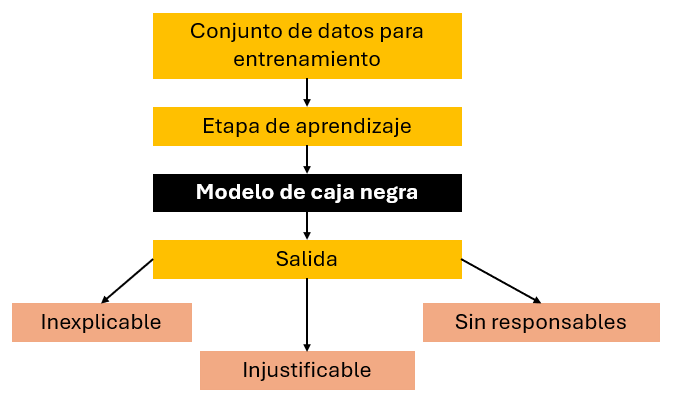
\includegraphics[width=0.7\linewidth]{modelo caja negra.png}
    \caption{Modelo de caja negra. Adaptado de
    \cite{hassija2024interpreting}.}
    \label{fig:caja negra}
\end{figure}
\end{comment}

No obstante, estos modelos también presentan algunas limitaciones. Debido a que dependen fuertemente de los datos utilizados para su identificación, su desempeño puede verse afectado cuando se aplican fuera del rango de operación considerado en la etapa de entrenamiento o calibración. Además, existe el riesgo de sobreajuste cuando se seleccionan estructuras con órdenes elevados o con una cantidad excesiva de parámetros, lo que puede llevar al modelo a reproducir el ruido presente en los datos en lugar de capturar la verdadera dinámica del sistema \cite{wallentinsson2020empirical}.


A continuación, se describen las principales técnicas de modelos dinámicos basados en datos identificadas en la literatura, considerando tanto enfoques lineales como no lineales. Estas metodologías permiten construir representaciones matemáticas a partir de registros experimentales de entrada y salida, sin requerir necesariamente una descripción física del sistema. La revisión se enfoca principalmente en modelos aplicados a sistemas térmicos, debido a que estos presentan, al igual que el sistema en estudio, dinámicas lentas, retardos de transporte y posibles comportamientos no estacionarios. No obstante, también se consideran técnicas desarrolladas en otros tipos de sistemas dinámicos, cuyos fundamentos pueden adaptarse al análisis, identificación y simulación de procesos térmicos.





\subsection{Técnicas de modelado lineales}




\subsubsection{Modelo autorregresivo con entrada exógena (ARX)}


De acuerdo con lo establecido en \cite{ljung1999system}, un modelo ARX de entrada única y salida única (SISO) describe la salida $y$ en el momento $k$ como una combinación lineal de valores pasados de la salida y de la entrada. De esta forma, la salida actual depende tanto de las salidas pasadas medidas del sistema como de entradas pasadas, permitiendo representar la dinámica temporal del proceso. La expresión general del modelo se define mediante parámetros lineales: 

\begin{equation}    \label{ecuacionARX}
    y(k)=-\sum\limits_{i=1}^{n_{a}} a_{i}y(k-i)+\sum\limits_{i=1}^{n_{b}} b_{i}u(k-i-n_{k}+1) +e(k) 
\end{equation}
    


donde:
\begin{itemize}
    \item $n_{a} \in \mathbb{N}$: Orden autorregresivo.
\item $n_{b} \in \mathbb{N}$: Orden exógeno.
\item $n_{k} \in \mathbb{N}$: Retardo entre entrada-salida.
\item $a_{i}$: El $i$ parámetro autorregresivo.
\item $b_{i}$: El $i$ parámetro exógeno.
\item $e(k)$: Perturbación o ruido.
\end{itemize}

La estructura polinomial del modelo ARX \cite{Muftah2021} puede expresarse como:

\begin{equation}    \label{ecuacionpolARX}
y(k)=\frac{B(q)}{A(q)}u(k)+\frac{1}{A(q)}e(k)
\end{equation}
donde:
\begin{itemize}
    \item $A(q)$: Polinomio autorregresivo.
    \item $B(q)$: Polinomio exógeno.
    
\end{itemize}
La Figura \ref{fig:ModeloARXestructura} muestra la representación estructural del modelo ARX. En esta estructura, la señal de entrada $u$ atraviesa el bloque dinámico $\frac{B(q)}{A(q)}$, mientras que el término de perturbación $e(k)$ es filtrado mediante el bloque $\frac{1}{A(q)}$. De esta manera, tanto la dinámica del sistema, como la dinámica del ruido comparten el mismo denominador $A(q)$, características distintiva de los modelos ARX. En consecuencia, las perturbaciones son afectadas por la misma dinámica asociada al proceso.

 \begin{figure}[h]
     \centering
     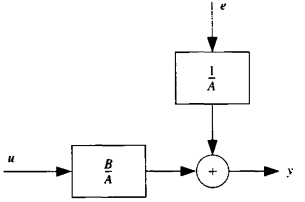
\includegraphics[width=0.5\linewidth]{Estructura ARX.png}
     \caption{Estructura del modelo ARX \cite{ljung1999system}.}
     \label{fig:ModeloARXestructura}
 \end{figure}
Asimismo, debido a la presencia del polinomio $A(q)$, el modelo incorpora una componente autorregresiva, utilizando salidas pasadas reales medidas experimentalmente para calcular las salidas futuras. Esta característica permite que el modelo posea una identificación relativamente simple y eficiente computacionalmente.
Finalmente, es importante destacar que la validez de este tipo de modelos se fundamenta en la suposición de que el sistema puede aproximarse como lineal e invariante en el tiempo (LTI), además de requerir condiciones de operación consistentes entre etapas de identificación y validación del modelo \cite{BARTHELEMY2025109971}.

Los modelos ARX han sido utilizados en diversas aplicaciones térmicas, tales como hornos térmicos industriales \cite{BARTHELEMY2025109971}, sistemas HVAC de edificios \cite{MUSTAFARAJ2010348}, modelación de invernaderos \cite{lopez2007modelos}, sistemas de transferencia de calor \cite{gunsha2023modelado} y predicción de radiación solar \cite{10.3389/fenrg.2022.822555}. Lo anterior deja en claro su amplia utilización en sistemas térmicos caracterizados por dinámicas lentas y dominadas por bajas frecuencias.
Otra ventaja relevante del modelo ARX corresponde a su interpretabilidad física y capacidad para realizar análisis dinámicos clásicos, tales como análisis de estabilidad, análisis espectral y estudio de la respuesta en frecuencia \cite{dong2025end}.
Asimismo, la  baja complejidad computacional del modelo ARX permite su implementación en tiempo real, aspecto relevante para aplicaciones de monitoreo, validación online y diseño de estrategias de control \cite{BARTHELEMY2025109971}.

\subsubsection{Modelo Output-Error (OE)}


La estructura del modelo Output Error \cite{Muftah2021} es representada por la Figura \ref{fig:estructuramodelooe}. En este esquema la salida medida $y$ se modela como la suma de un parte determinística generada por la dinámica del sistema y un término de perturbación o ruido ($e$).

\begin{figure}[H]
    \centering
    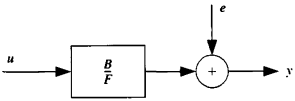
\includegraphics[width=0.5\linewidth]{Estructura OE.png}
    \caption{Estructura modelo OE \cite{ljung1999system}.}
    \label{fig:estructuramodelooe}
\end{figure}
También, puede ser expresado mediante \cite{Muftah2021} :

\begin{equation}    \label{ecuacionOE}
y(k)=\frac{B(q)}{F(q)}u(k)+e(k)
\end{equation}
donde:
\begin{itemize}
    \item $u(t)$: Señal de entrada del sistema.
    \item $y(t)$: Salida medida.
    \item $\frac{B(q)}{F(q)}$: Función de transferencia discreta.
    \item $e(t)$ Ruido o perturbación.
    \item $q$: Operador de retardo discreto.
    
\end{itemize}
En el modelo OE, la dinámica del sistema está contenida en la función de transferencia $\frac{B(q)}{F(q)}$, mientras que el ruido se considera como una perturbación aditiva sobre la salida, sin dinámica asociada, lo cual diferencia a este modelo de otras estructuras, como ARX, donde el  ruido también posee una representación dinámica \cite{ljung1999system}.
Además, el modelo OE utiliza las salidas pasadas generadas por el propio modelo para calcular la salida actual del sistema. Esto ocurre debido a la presencia del polinomio denominar $F(q)$, el cual introduce una retroalimentación interna de las salidas simuladas. En consecuencia, el modelo evoluciona utilizando únicamente sus propias predicciones pasadas. Esto, convierte al modelo OE en una estructura particularmente exigente desde el punto de vista de validación dinámica, ya que los errores de modelación pueden propagarse y acumularse a lo largo del tiempo \cite{ljung1999system}.
Asimismo, en \cite{tangirala2018principles} se señala que los modelos OE concentran el modelado en la función de transferencia del sistema, evitando incorporar explícitamente dinámica del ruido en la estructura del modelo.

Se ha reportado el uso favorable de estructuras OE en distintos sistemas dinámicos. Por ejemplo, un estudio comparó distintas estructuras paramétricas de identificación para modelar un actuador neumático inteligente, observando que las estructuras OE lograron desempeños superiores al 90\% de ajuste, mostrando una adecuada capacidad para representar dinámicas complejas \cite{Muftah2021}. Adicionalmente, \cite{stojanovic2014adaptive} y \cite{STOJANOVIC2016576} destacan las ventajas de esta estructura cuando se busca mejorar la precisión dinámica mediante diseños de excitación adecuados, como señales PRBS o estrategias óptimas de entrada. Allí también se enfatiza que los modelos Output-Error permiten concentrar la identificación sobre la dinámica física del sistema, logrando estimaciones consistentes y una mejor representación de la relación dinámica entrada-salida.

\subsubsection{Modelo Box-Jenkins (BJ)}


El modelo Box-Jenkins o BJ es una estructura paramétrica lineal utilizada en identificación de sistemas, caracterizada por representar de manera independiente la dinámica del sistema y la dinámica del ruido mediante funciones racionales distintas \cite{mu2026sequentiallydecouplingestimatorsboxjenkins}. A diferencia de estructuras como el modelo ARX, en el cual la dinámica del sistema y la del ruido comparten parcialmente la misma estructura polinomial y del modelo OE, que no incorpora explícitamente un modelo para el ruido, el modelo BJ desacopla completamente ambas dinámicas. Esta característica le otorga una mayor flexibilidad para representar procesos afectados por perturbaciones, ruido de medición o fenómenos no modelados \cite{ljung1999system}.

\begin{figure}[H]
    \centering
    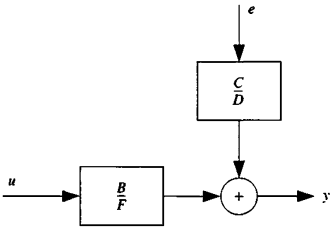
\includegraphics[width=0.5\linewidth]{modeloBJ.png}
    \caption{Estructura del modelo Box-Jenkins \cite{ljung1999system}.}
    \label{fig:modeloBJestructura}
\end{figure}

La estructura presentada en la Figura \ref{fig:modeloBJestructura} puede expresarse matemáticamente como:

\begin{equation}    \label{ecuacionBJ}
y(k)=\frac{B(q)}{F(q)}u(k)+\frac{C(q)}{D(q)}e(k)
\end{equation}
donde:
\begin{itemize}
    \item $\frac{B(q)}{F(q)}$ representa la dinámica determinística entre la entrada y la salida.
    \item $\frac{C(q)}{D(q)}$ describe la dinámica estocástica asociada al ruido o perturbación.
\end{itemize}
De esta forma, el modelo BJ puede interpretarse como la combinación de dos submodelos racionales: uno asociado a la relación determinística entre la entrada y salida y otro destinado a representar la estructura estocástica del ruido o perturbaciones presentes en los datos. En consecuencia, la estimación del modelo consiste en determinar los parámetros de los polinomios $B(q)$, $F(q)$, $C(q)$ y $D(q)$ a partir de registros experimentales de entrada y salida, buscando representar de forma adecuada tanto la dinámica del proceso como la dinámica del error \cite{mu2026sequentiallydecouplingestimatorsboxjenkins}. Además, el enfoque Box-Jenkins puede entenderse como un procedimiento iterativo compuesto por las etapas de identificación, estimación y verificación, donde la validación mediante análisis de residuos permite evaluar si la estructura seleccionada ha capturado la información dinámica relevante del sistema \cite{RO_1977__11_1_3_0}.

El uso de modelos BJ ha sido reportado favorablemente en aplicaciones relacionadas con sistemas térmicos y procesos dinámicos. Abirami y Sivagamasundari \cite{Abirami2018STHX}, al modelar un intercambiador de calor de tubos y coraza mediante técnicas de identificación de sistemas, concluyen que el modelo BJ presentó mejores resultados en términos de porcentaje de ajuste, error de predicción final, función de costo y análisis de correlación, en comparación con otras estructuras como OE. Asimismo, en \cite{gunsha2023modelado} se concluye que, para un sistema de transferencia de calor de una ducha eléctrica excitado mediante señales PRBS, el modelo Box-Jenkins obtuvo el mayor porcentaje de estimación respecto de otros modelos paramétricos evaluados. De la misma forma, en el artículo de modelado de un actuador neumático \cite{Muftah2021} el modelo Box-Jenkins obtiene un 91.24\% de ajuste, superior al umbral exigido por el autor, demostrando un buen desempeño. Esto evidencia que la estructura BJ puede entregar una representación adecuada en sistemas dinámicos donde la relación entrada-salida y la dinámica del error requieren ser tratadas con mayor flexibilidad.



\subsection{Técnicas de modelado no lineales}
\subsubsection{Mejor aproximación lineal (BLA)}

Es un marco de estimación no paramétrica no lineal y semi automático diseñado para mediciones vibroacústicas industriales con múltiples entradas y multiples salidas (MIMO). Se define como un enfoque de modelado que busca minimizar el error cuadrático medio entre la salida verdadera de un sistema no lineal y la salida de un modelo lineal asociado. En otras palabras, la BLA es la mejor aproximación lineal que representa un sistema no lineal en términos de minimizar la discrepancia media cuadrática con la salida real del sistema. Su propósito es la ayuda a usuarios, incluidos los no expertos, a tomar decisiones informadas sobre la linealidad de un sistema. Permite identificar si un sistema es lineal, si un marco lineal es lo suficientemente preciso y cuánto se puede ganar utilizando un marco no lineal avanzado \cite{csurcsia2020user} . Algunas características de la BLA son las siguientes \cite{schoukens2017identification}: 
\begin{enumerate}
    \item \textbf{Punto de partida para modelado no lineal:} Actúa como una representación inicial del sistema no lineal.
    \item \textbf{Separación de dinámica y no linealidad:} En muchos modelos, la dinámica del sistema está contenida en los bloques lineales, mientras que las distorsiones están en los bloques no lineales. La BLA permite aislar la parte dinámica observable desde el exterior.
    \item \textbf{Útil en presencia de ruido:} Permite estimaciones robustas y consistentes aún en sistemas ruidosos, usando técnicas como mínimos cuadrados en el dominio de la frecuencia.
    \item \textbf{Dependencia de la señal de entrada:} La forma que toma la BLA depende de las propiedades estadísticas de la señal de excitación, por ejemplo su varianza, espectro y distribución.
\end{enumerate}


\subsubsection{Modelo Hammerstein}


Este modelo está compuesto por una no linealidad estática seguida de un sistema lineal invariante en el tiempo (LTI o \textit{Linear Time-Invariant} en inglés). Es decir, la señal de entrada pasa primero por una transformación no lineal sin memoria y luego por una dinámica lineal que representa el comportamiento temporal del sistema. Esta estructura es útil para modelar sistemas donde las no linealidades se encuentran en la entrada, como en actuadores o procesos físicos con características no lineales no tan complejas.
El modelo Hammerstein es considerado un aproximador universal para sistemas con memoria de desvanecimiento (\textit{fading memory}), es decir, sistemas cuya respuesta depende de entradas pasadas, pero donde dicha influencia decrece con el tiempo. Sin embargo, su capacidad para representar dinámicas complejas o múltiples interacciones internas es limitada. Desde el punto de vista de identificación, una estrategia común consiste en:
\begin{enumerate}
    \item Estimar la parte lineal \textit{S(q)} utilizando BLA, que captura la dinámica dominante del sistema bajo ciertas condiciones de entrada.
    \item Luego, identificar la no linealidad \textit{f(u)} mediante una expansión en funciones base (por ejemplo, polinomios) usando un enfoque lineal en los parámetros como mínimos cuadrados, lo que permite una implementación eficiente \cite{schoukens2017identification}.
\end{enumerate}
 En la Figura \ref{fig:enter-label} se representa el modelo Hammerstein donde \textit{f(u)} corresponde al bloque de no linealidad estática y \textit{S(q)} al sistema LTI que define la dinámica del sistema.
\begin{figure}[h!]
    \centering
    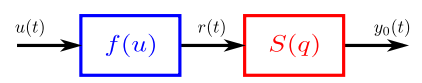
\includegraphics[width=0.5\linewidth]{modelo Hammerstein.png}
    \caption{Estructura en bloque del modelo Hammerstein
    \cite{schoukens2017identification}.}
    \label{fig:enter-label}
\end{figure}

\subsubsection{Modelo Wiener}

El modelo Wiener está conformado por un bloque lineal invariante en el tiempo (LTI) \textit{G(q)} seguido por una no linealidad estática \textit{g(x)}. En esta estructura, la señal de entrada es primero procesada por una dinámica lineal que modela la respuesta temporal del sistema y luego transformada por una función no lineal sin memoria. Este tipo de modelo es particularmente adecuado para representar sistemas donde las no linealidades se manifiestan en la salida, como en sensores no lineales o válvulas de sobreflujo.

El modelo Wiener, al igual que el Hammerstein, pertenece a la clase de sistemas con memoria de desvanecimiento, por lo que puede capturar dinámicas temporales limitadas. Sin embargo, su capacidad de representación es restringida cuando se trata de sistemas con interacciones no lineales complejas o múltiples componentes dinámicos.

Para su identificación, se emplea una estrategia en dos etapas:
\begin{enumerate}
    \item Se estima el bloque LTI \textit{G(q)} utilizando BLA, que proporciona una representación efectiva de la dinámica del sistema bajo un cierto régimen de excitación.
    \item A partir de la salida del bloque lineal, se ajusta el bloque no lineal \textit{g(x)} mediante un modelo adecuado (por ejemplo, una expansión polinomial o una red neuronal), normalmente utilizando un enfoque lineal en los parámetros.
\end{enumerate}
Esta estructura permite separar claramente la identificación de la parte dinámica y de la no linealidad, facilitando su implementación y reduciendo la complejidad computacional \cite{schoukens2017identification}.
La Figura \ref{fig:enter-label2} muestra el modelo Wiener en bloque. 
\begin{figure}[H]
    \centering
    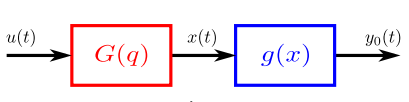
\includegraphics[width=0.5\linewidth]{modelo Wiener.png}
    \caption{Estructura en bloque del modelo Wiener
    \cite{schoukens2017identification}.}
    \label{fig:enter-label2}
\end{figure}
\subsubsection{Modelo Wiener–Hammerstein}

 El modelo Wiener-Hammerstein está compuesto por una no linealidad estática \textit{f(x)} ubicada entre dos bloques lineales invariantes en el tiempo \textit{G(q)} y \textit{S(q)}. Esta estructura se utiliza para representar sistemas en los que la dinámica ocurre tanto antes como después del comportamiento no lineal. Según la referencia  \cite{schoukens2017identification}, uno de los principales desafíos en la identificación de este modelo es separar adecuadamente las dinámicas de los dos bloques lineales, ya que la mejor aproximación lineal (BLA) del sistema es proporcional al producto de \textit{G(q)} y \textit{S(q)}. Para resolver esta dificultad, se propone analizar las características dinámicas identificadas en la BLA y distribuir de manera adecuada los componentes responsables del comportamiento dinámico del sistema entre los dos bloques lineales del modelo. Esto se realiza mediante la evaluación de múltiples combinaciones posibles, estimando en cada caso la no linealidad intermedia y seleccionando la que minimiza el error cuadrático. Aunque este procedimiento ofrece estimaciones consistentes, se recomienda aplicar una optimización no lineal posterior para refinar los parámetros del modelo, especialmente en configuraciones con mayor complejidad estructural.
La Figura \ref{fig:enter-label5} representa al modelo Wiener-Hammerstein, donde la entrada \textit{u(t)} pasa primero por un bloque lineal dinámico \textit{G(q)}, luego atraviesa una no linealidad estática \textit{f(x)} y finalmente, la señal se procesa mediante otro bloque lineal dinámico \textit{S(q)} para generar la salida \textit{y(t)}.
 \begin{figure}[h!]
     \centering
    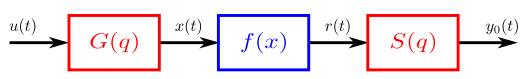
\includegraphics[width=0.7\linewidth]{Screenshot_3.png}
     \caption{Modelo Wiener-Hammerstein
    \cite{schoukens2017identification}.}
     \label{fig:enter-label5}
 \end{figure}

\subsubsection{Modelo Hammerstein-Wiener}

El modelo Hammerstein-Wiener combina una no linealidad en la entrada \textit{f(u)}, un bloque dinámico lineal \textit{G(q)} y una segunda no linealidad estática en la salida \textit{g(r)}, como se observa en la Figura \ref{fig:enter-label6}. Esta configuración le otorga una mayor flexibilidad para representar sistemas con comportamientos altamente no lineales, ya que permite modelar distorsiones tanto en la entrada como en la salida del proceso. A diferencia de los modelos Hammerstein o Wiener clásicos, la identificación de esta estructura es más compleja, debido a que la presencia de dos no linealidades afecta la distribución estadística de las señales internas, dificultando extraer directamente la dinámica del sistema a partir del la BLA. Así, el artículo \cite{schoukens2017identification} sugiere utilizar señales de entrada con una amplitud suficientemente pequeña para explorar el comportamiento lineal local, permitiendo obtener una estimación inicial del bloque dinámico central \textit{G(q)}. A partir de esta estimación, se identifican las no linealidades de entrada y salida mediante métodos como los mínimos cuadrados totales. No obstante, dado que este procedimiento no garantiza consistencia en presencia de ruido, se recomienda una optimización no lineal conjunta posterior para ajustar todos los parámetros del modelo de forma más precisa.

\begin{figure}[H]
    \centering
    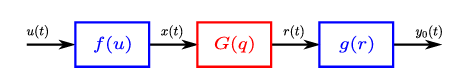
\includegraphics[width=0.5\linewidth]{hammersteinwiener.png}
    \caption{Modelo Hammerstein-Wiener
    \cite{schoukens2017identification}.}
    \label{fig:enter-label6}
\end{figure}

\subsubsection{Redes neuronales artificiales (ANN)} 
Son una técnica de aprendizaje autónomo perteneciente al campo de la IA, inspiradas en sistemas neuronales biológicos. Estas redes se basan en la composición de funciones no lineales, y al incorporar múltiples capas intermedias (redes profundas), pueden representar eficientemente funciones de alta complejidad \cite{duraisamy2019turbulence}. Se utilizan ampliamente en la predicción de consumo energético en edificios, donde deben abordar problemas con incertidumbres, no linealidades y diferentes horizontes de pronóstico. Gracias a su arquitectura, las ANN pueden gestionar modelos predictivos complejos. Sin embargo, su rendimiento está directamente vinculado al conjunto de datos con el que son entrenadas, lo que limita su capacidad de generalización a otros contextos o condiciones distintas \cite{BALALI2023113496}. Además, se aplican en el modelado de fenómenos altamente no lineales como la turbulencia, siendo capaces de aproximar funciones desde estructuras simples con una sola capa hasta configuraciones profundas con múltiples capas ocultas \cite{duraisamy2019turbulence}.


\subsubsection{Modelo de regresión de procesos Gaussianos (GPR)}

Es una técnica estadística no paramétrica utilizada para modelar funciones complejas e inciertas en el contexto del aprendizaje automático. Según Duraisamy et al. \cite{duraisamy2019turbulence}, el GPR se ha aplicado eficazmente en el modelado de discrepancias en turbulencias, particularmente para mejorar predicciones realizadas por modelos tradicionales como RANS (Reynolds-Averaged Navier–Stokes), una técnica ampliamente utilizada para representar flujos turbulentos. En este enfoque, la discrepancia entre el modelo físico y los datos de referencia se representa como una función aleatoria continua que asigna a cada punto del dominio una estimación incierta, pero con un comportamiento matemático bien definido: se supone que estos valores siguen una distribución normal (gaussiana) y están correlacionados entre sí según su proximidad y otras propiedades del flujo. Esta función se entrena utilizando datos de alta fidelidad obtenidos mediante simulaciones numéricas directas (DNS), las cuales resuelven todas las escalas del movimiento turbulento de un fluido sin necesidad de modelos de cierre, proporcionando resultados extremadamente precisos aunque computacionalmente costosos. La metodología se formula dentro de un marco bayesiano, lo que permite incorporar conocimiento previo sobre el modelo y actualizarlo con los datos observados, generando una predicción que no solo incluye el valor esperado de la corrección, sino también su grado de incertidumbre. En el documento, se ejemplifica este enfoque con estudios que utilizan GPR para aprender funciones de corrección, como la anisotropía del tensor de esfuerzos de Reynolds, en función de variables representativas del flujo, lo que permite mejorar la precisión de los modelos RANS sin alterar su estructura física \cite{duraisamy2019turbulence}.

\begin{comment}
 
\subsubsection{Técnicas de Deep Learning o Aprendizaje Profundo }
    
Desarrollados en base a redes neuronales con mayor flexibilidad en los tipos de datos. Han mostrado mayor precisión de predicción que las técnicas ANN simples en algunos estudios. 
    
 \subsubsection{Redes neuronales de retraso de tiempo (TDNN)}
 Incluyen el estado en tiempo real de las variables de entrada y sus estados anteriores, con la capacidad de almacenar información retrasada \cite{BALALI2023113496}. 
        

  \subsubsection{Modelo Híbrido PDNN (Process Dynamics-Guided Neuronal Network)}
Red neuronal artificial mejorada que incorpora el conocimiento de la dinámica del proceso y la experiencia del campo para mejorar la capacidad de generalización del modelo. A diferencia de los modelos puramente basados en datos o empíricos, que se basan únicamente en los datos de entrada, el PDNN integra el conocimiento intrínseco del sistema para aprender relaciones y predecir resultados. Fue desarrollado para mejorar la generalización del modelo y mantener un rendimiento superior, incluso con datos escasos o de baja calidad, lo que es crucial en sistemas complejos de procesamiento químico, donde obtener datos de alta fidelidad, en cantidad y granularidad suficientes, es un desafío debido a múltiples fallas, paradas del proceso, fluctuaciones aleatorias y errores en la entrada de datos.
El PDNN se distingue del ANN estándar por la adición de una capa adicional en su arquitectura, denominada capa de información del proceso, la cual integra explícitamente el conocimiento del proceso y la experiencia del dominio. Este conocimiento puede ser de cuatro niveles:
\begin{itemize}
    \item Nivel 1 (leyes de conservación): Incluye leyes fundamentales como el balance de masa y energía, y leyes universales, que son estrictamente seguidas por cualquier sistema o subsistema industrial.
    \item Nivel 2 (regulaciones y restricciones): Captura regulaciones sobre emisiones, limites superiores de regiones tolerables y límites en parámetros físicos como la densidad.
    \item Nivel 3 (dinámica del proceso y operaciones): Detalla operaciones como reacción, separación, intercambio de calor y tratamiento de residuos, incorporando ecuaciones complejas como ecuaciones diferenciales parciales, correlaciones fundamentales y ecuaciones no lineales.
    \item Nivel 4 (heurísticas y ergonomía): Aborda la desalineación entre personas, herramientas y entornos de trabajo y puede ayudar a diseñar modelos basados en datos con heurísticas de diseño rápidas y de bajo costo.
\end{itemize}

El modelo aprende ajustando sus parámetros en un ciclo iterativo. Primero, realiza predicciones a partir de los datos de entrada (propagación hacia delante). Luego, compara esas predicciones con los valores reales usando una función de error. Posteriormente, ajusta los pesos de la red para reducir ese error (retropropagación), repitiendo este proceso hasta que las predicciones sean suficientemente buenas. En redes con conocimiento del proceso, algunos pesos pueden modificarse específicamente para reflejar ese conocimiento, lo que mejora también el aprendizaje \cite{ALAUDDIN2023158}. 
\end{comment}  
\subsubsection{ Modelo autorregresivo no lineal con entrada exógena (NARX)}

El modelo autorregresivo no lineal con entrada exógena corresponde a una estructura de modelado dinámico utilizada para representar sistemas no lineales a partir de datos. Este tipo de modelo estima la salida de un sistema considerando tanto valores pasados de la propia salida como valores pasados de una o más entradas externas o exógenas. De esta manera, incorpora memoria dinámica y permite describir procesos donde la respuesta actual depende de la evolución previa del sistema y de las señales de entrada aplicadas \cite{BALALI2023113496}.

El modelo NARX relaciona valores actuales y pasados de varias series temporales, recibiendo variables dinámicas provenientes de distintas señales. En su formulación general, la salida estimada se expresa mediante una función no lineal $f(\cdot)$, que relaciona los valores pasados de la salida y de entradas exógenas, además de un término de error \cite{montero2024modelo}.

En términos generales, un modelo NARX puede representarse como:

\begin{equation}    \label{ecuacionNARX}
{\hat{y}}=f[y(k-1),...,y(k-n_a),u_1(k-nk_1),...,u_1(k-nk_1-n_{b1}+1,u_2(k-nk_2),...,u_2(k-nk_2-n_{b2}+1)]
\end{equation}
donde:
\begin{itemize}
    \item $\hat{y}$ : Salida estimada.
    \item $y(k-i)$ : Valores pasados de la salida.
    \item $u_1$ y $u_2$ : Entradas exógenas.
    \item $n_a$ : Orden autorregresivo.
    \item $n_b$ : Retardos de cada entrada.
    \item $n_k$ : Retardo de cada entrada respecto a la salida.
    \item $f(\cdot)$ : Función no lineal.
\end{itemize}

La función $f(\cdot)$ puede aproximarse mediante distintas técnicas de identificación no lineal, como redes neuronales, funciones polinomiales o métodos de aprendizaje automático \cite{barbosa2010tecnicas}, \cite{montero2024modelo}.

Se ha utilizado en la detección y diagnóstico de fallos en sistemas termodinámicos, particularmente en la trayectoria de gases de turbina y sus componentes, también en el comportamiento termodinámico a corto plazo en edificios \cite{zhou2024review} y en la predicción de temperaturas en un horno industrial \cite{montero2024modelo}.

Ofrece ventajas en la simulación de sistemas complejos con una no linealidad significativa. A menudo se combinan redes neuronales para mejorar su capacidad de diagnóstico de fallos y simular las características dinámicas. Dentro de sus limitaciones está la necesidad de grandes cantidades de datos de entrenamiento de alta calidad \cite{zhou2024review}.

\subsubsection{ Modelo de ecuaciones diferenciales ordinarias neuronales}

Una red neuronal ODE o Neural Differential Equation en inglés, es un modelo de aprendizaje profundo diseñado para representar sistemas dinámicos en tiempo continuo. A diferencia de una red neuronal convencional, donde la transformación de la información ocurre mediante una secuencia discreta de capas, una ODE neuronal parametriza mediante una red neuronal la derivada del estado del sistema. De esta forma la evolución temporal del estado se describe mediante una ecuación diferencial ordinaria cuya dinámica es aprendida desde los datos \cite{chen2018neural}. 

En términos generales, el modelo puede expresarse como:

\begin{equation}    \label{ecuacionODENEUROA}
\frac{dx(t)}{dt}=f(x(t),u(t),t)
\end{equation}
donde:
\begin{itemize}
    \item $x(t)$ : Estado del sistema.
    \item $u(t)$ : Entradas externas.
    \item $t$ : Tiempo.
    \item $f(\cdot)$ : Red neuronal.
\end{itemize}
Los parámetros de la red neuronal son ajustados durante el entrenamiento. La salida del modelo se obtiene resolviendo numéricamente esta ecuación diferencial mediante un integrador EDO.

En la Figura \ref{fig:NeuralODEvs} se compara una red residual con una red neuronal ODE, mostrando dos formas distintas de transformar un estado desde la entrada hacia la salida. En la red residual, a la izquierda, la evolución ocurre mediante una secuencia discreta de capas o bloques, donde la profundidad corresponde al avance capa por capa dentro de la red. El estado se actualiza de la manera en la que se visualiza en las trayectorias negras, las cuales avanzan mediante saltos entre profundidades discretas. En cambio, en la red neuronal EDO, mostrado a la derecha, la profundidad se interpreta como una variable continua, análoga al tiempo, donde la evolución del estado se describe mediante una ecuación diferencial ordinaria. Así, la red neuronal no define directamente una nueva capa, sino un campo vectorial, obteniendo las trayectorias negras continuas. Por ello, el modelo neuronal ODE puede interpretarse como una generalización continua de una red residual, donde la secuencia finita de capas es reemplazada por la integración numérica de una EDO parametrizada por una red neuronal.

\begin{figure}[H]
    \centering
    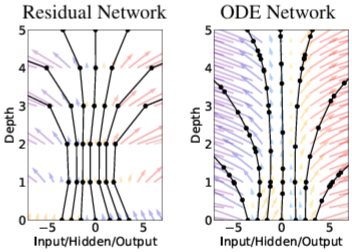
\includegraphics[width=0.5\linewidth]{NeuralODE.png}
    \caption{Red neuronal artificial profunda comparada con un red neuronal EDO \cite{chen2018neural}.}
    \label{fig:NeuralODEvs}
\end{figure}






\subsubsection{Resumen de la sección}
Con el propósito de facilitar la comparación entre los modelos y técnicas descritos anteriormente, en la Tabla \ref{tab:modelos-datos} se presenta una síntesis comparativa de sus principales características. En ella se incluyen las aplicaciones típicas de cada modelo, sus principales ventajas, sus limitaciones y una estimación cualitativa de su complejidad de implementación.

\begin{comment}
    

\subsection{Modelos Híbridos o de Caja Gris}


El modelo de caja gris representa una estrategia de modelado intermedia que combina el conocimiento físico del sistema con datos experimentales, integrando así las fortalezas de los modelos de caja blanca (basados en leyes físicas) y caja negra (basados únicamente en datos). Este enfoque ha ganado reconocimiento por su capacidad para capturar dinámicas térmicas complejas con una estructura interpretativa y  exigencia computacional reducida. En el contexto del modelado energético de edificios, se considera una alternativa prometedora para enfrentar los desafíos derivados del uso de sensores, la incertidumbre de los datos y la complejidad de los sistemas dinámicos reales, aportando flexibilidad, precisión y robustez en condiciones variables \cite{BALALI2023113496}. 
El modelo de caja gris es generalmente más interpretable que el modelo de caja negra, al mismo tiempo que más simple y eficiente computacionalmente que un modelo físico completo (caja blanca). Su principal exponente es el modelo RC (Resistencia-Capacitancia). también conocido como el modelo de red térmica, que utiliza la analogía eléctrica para representar los procesos térmicos en edificios. En este modelo, las resistencias térmicas (R) simulan las barreras al flujo de calor, mientras que las capacitancias térmicas (C) representan la capacidad de los materiales para almacenar energía. Estas configuraciones pueden estructurarse con distintos niveles de detalle, como 1R1C, 3R2C o 5R1C, dependiendo del número de elementos utilizados y pueden aplicarse tanto a componentes individuales (muros o ventanas) como a zonas o edificios multizona.

Entre sus principales ventajas, el modelado de caja gris permite preservar las propiedades físicas esenciales del sistema térmico, facilita una rápida estimación de cargas térmicas y es especialmente eficaz en aplicaciones de control predictivo ( como MPC, Modelo de Control Predictivo), optimización energética, simulación urbana y modelado de integración edificio-red eléctrica. Al poder ser modelado mediante ecuaciones que describen su evolución temporal en función de entradas y salidas, puede integrarse fácilmente en estrategias avanzadas de control y gestión energética en tiempo real \cite{Li2021GreyBox}. 


No obstante, el modelo de caja gris también presenta limitaciones. La referencia utilizada \cite{Li2021GreyBox} destaca varios desafíos que dificultan su adopción más amplia:
\begin{enumerate}
    \item Falta de claridad teórica en las suposiciones y limitaciones del modelo.
    \item Ausencia de una convención estandarizada en la nomenclatura y estructura, por ejemplo, el modelo 3R2C puede referirse a una pared o a una zona, dependiendo del autor.
    \item Escasa claridad sobre sus aplicaciones más adecuadas.
    \item Limitado soporte de software, ya que no existen herramientas genéricas, robustas y accesibles que faciliten su implementación sistemática.
    
\end{enumerate}
\end{comment}
\begin{comment}
    


\begin{itemize}
 

    \item \textbf{Aprendizaje por Refuerzo (RL)}
    
    Esta técnica se basa en un marco de proceso de decisión de Markov (MDP), donde el siguiente estado del sistema depende solo del estado actual, independientemente de los estados anteriores \cite{buildings14030833}. Esta técnica se utiliza  en el documento "Dynamic Modeling of Heat Exchangers Bases on Mechanism and Reinforcement Learning Synergy" \cite{buildings14030833} para la determinación en tiempo real del coeficiente global de transferencia de calor (U) en un intercambiador de calor, utilizando también el algoritmo \textit{Deep Deterministic Policy Gradient} (DDPHG), adecuado para problemas con espacios de acción continuos y sistemas complejos no lineales. Este algoritmo utiliza una estructura Actor-Critic y un mecanismo de Experiencia Repetida para mejorar su rendimiento y estabilidad.
\begin{itemize}
    \item La red Actor recibe las variables de estado observadas (en este caso temperatura y caudal de entrada) y produce la acción, que es la selección del valor de U
    \item La red Critic ayuda a la red anterior a aprender mejores estrategias.
    \item La Experiencia Repetida almacena la información (estado actual, acción, recompensa, siguiente estado) para estabilizar el entrenamiento y mejorar la eficiencia de la muestra.
\end{itemize}

Se utiliza un sistema para recopilar datos operativos en tiempo real de caudales y temperaturas en ambos lados del intercambiador de calor. Los datos brutos se pre-procesan para mejorar su calidad, pues pueden contener valores atípicos y faltantes.

Componentes del proceso de RL:
\begin{itemize}
    \item Agente inteligente: Cerebro del proceso, compuesto por una red neuronal y responsable de registrar las variables de estado, recibir la recompensa en tiempo real  y ajustar sus acciones (el valor de U) \cite{BALALI2023113496}.
    \item Entorno: Proporciona una retroalimentación al agente sobre las variables de estado actuales. En este caso corresponde a la unidad del intercambiador de calor, que se describe mediante ecuaciones mecanicistas y los datos operativos importados.
    \item Estado: Los parámetros claves del modelo mecanicista, incluyendo temperaturas del fluido frío y caliente, caudales y la diferencia de temperatura media logarítmica (LMTD).
    \item Acción: Un parámetro dinámico a identificar, siendo el coeficiente global de transferencia de calor en este estudio.
    \item Función de recompensa: Construida a partir del error relativo entre el LMTD de salida del modelo y el LMTD  real medido. Un error relativo menor resulta en una recompensa mayor \cite{buildings14030833}.
\end{itemize}

El modelo resultante de este artículo demostró una alta precisión de identificación, con un error relativo promedio inferior al 5\% \cite{buildings14030833}. 
\end{itemize}


\end{comment}



\begin{table}[H]
\caption{Tabla comparativa de modelos basados en datos.}
\label{tab:modelos-datos}
\centering
\resizebox{\textwidth}{!}{%
\begin{tabular}{|l|l|l|l|l|}
\hline
\textbf{Modelo} & \textbf{Aplicación típica} & \textbf{Ventajas} & \textbf{Limitaciones} & \textbf{Complejidad} \\ \hline

\textbf{ARX} &
\begin{tabular}[c]{@{}l@{}}Identificación de sistemas lineales\\ dinámicos SISO o MISO.\end{tabular} &
\begin{tabular}[c]{@{}l@{}}Estructura simple.\\ Bajo costo computacional.\end{tabular} &
\begin{tabular}[c]{@{}l@{}}La dinámica y el ruido comparten \\ el mismo denominador.\\ Limitado a sistemas aproximadamente LTI.\end{tabular} &
Baja \\ \hline

\textbf{OE} &
\begin{tabular}[c]{@{}l@{}}Modelado de la dinámica determinística\\ entrada-salida.\end{tabular} &
\begin{tabular}[c]{@{}l@{}}No modela explícitamente la dinámica\\ del ruido.\\ Adecuado para simulación libre.\end{tabular} &
\begin{tabular}[c]{@{}l@{}}Los errores pueden propagarse en\\ simulación libre.\end{tabular} &
Media \\ \hline

\textbf{Box-Jenkins} &
\begin{tabular}[c]{@{}l@{}}Sistemas afectados por perturbaciones o\\ ruido de medición\end{tabular} &
\begin{tabular}[c]{@{}l@{}}Separa la dinámica del sistema\\ y la dinámica del ruido.\\ Alta flexibilidad estructural.\end{tabular} &
\begin{tabular}[c]{@{}l@{}}Mayor complejidad de identificación.\\ Requiere selección adecuada de varios\\ órdenes.\end{tabular} &
Alta \\ \hline

\textbf{BLA} &
\begin{tabular}[c]{@{}l@{}}Punto de partida para modelos\\ no lineales.\end{tabular} &
\begin{tabular}[c]{@{}l@{}}Separa dinámica y no linealidad.\\ Robusta ante ruido.\end{tabular} &
\begin{tabular}[c]{@{}l@{}}Depende de la señal de entrada.\\ No representa completamente\\ las no linealidades.\end{tabular} &
Baja \\ \hline

\textbf{Hammerstein} &
\begin{tabular}[c]{@{}l@{}}Actuadores o sistemas físicos\\ con no linealidad en la entrada.\end{tabular} &
\begin{tabular}[c]{@{}l@{}}Estructura simple.\\ Aproximador universal para sistemas\\ con memoria de desvanecimiento.\end{tabular} &
\begin{tabular}[c]{@{}l@{}}Limitado para dinámicas complejas\\ o múltiples interacciones internas.\end{tabular} &
Media \\ \hline

\textbf{Wiener} &
\begin{tabular}[c]{@{}l@{}}Sensores, válvulas o sistemas con\\ no linealidad en la salida.\end{tabular} &
\begin{tabular}[c]{@{}l@{}}Separa la dinámica\\ lineal y la no linealidad estática.\end{tabular} &
\begin{tabular}[c]{@{}l@{}}Capacidad restringida ante sistemas\\ con interacciones no lineales complejas.\end{tabular} &
Media \\ \hline

\textbf{\begin{tabular}[c]{@{}l@{}}Wiener-\\ Hammerstein\end{tabular}} &
\begin{tabular}[c]{@{}l@{}}Sistemas con dinámica antes y\\ después de una no linealidad.\end{tabular} &
\begin{tabular}[c]{@{}l@{}}Captura comportamientos más complejos\\ que Hammerstein o Wiener simples.\end{tabular} &
\begin{tabular}[c]{@{}l@{}}Dificultad para separar correctamente\\ los dos bloques dinámicos lineales.\end{tabular} &
Alta \\ \hline

\textbf{\begin{tabular}[c]{@{}l@{}}Hammerstein-\\ Wiener\end{tabular}} &
\begin{tabular}[c]{@{}l@{}}Sistemas altamente no lineales con\\ distorsiones en entrada y salida.\end{tabular} &
\begin{tabular}[c]{@{}l@{}}Alta flexibilidad de modelado.\\ Permite representar no linealidades\\ de entrada y salida.\end{tabular} &
\begin{tabular}[c]{@{}l@{}}Identificación más compleja.\\ Requiere optimización no lineal conjunta\\ para refinar parámetros.\end{tabular} &
Alta \\ \hline


\textbf{GPR} &
\begin{tabular}[c]{@{}l@{}}Modelado de funciones complejas e inciertas.\\ Discrepancias entre modelos físicos\\ y datos de alta fidelidad.\end{tabular} &
\begin{tabular}[c]{@{}l@{}}Incorpora incertidumbre.\\ Marco bayesiano.\\ Adecuado para datos de alta fidelidad.\end{tabular} &
\begin{tabular}[c]{@{}l@{}}Alto costo computacional.\\ Requiere datos representativos\\ y de alta calidad.\end{tabular} &
Alta \\ \hline



\textbf{NARX} &
\begin{tabular}[c]{@{}l@{}}Sistemas dinámicos no lineales con\\ entradas exógenas.\\ Diagnóstico de fallos y predicción\\ de temperatura.\end{tabular} &
\begin{tabular}[c]{@{}l@{}}Incorpora memoria dinámica.\\ Usa salidas y entradas pasadas.\\ Adecuado para procesos no lineales.\end{tabular} &
\begin{tabular}[c]{@{}l@{}}Requiere datos de entrenamiento\\ de alta calidad.\\ Sensible a la selección de órdenes\\ y retardos.\end{tabular} &
Alta \\ \hline

\textbf{\begin{tabular}[c]{@{}l@{}}EDO\\ neuronal\end{tabular}} &
\begin{tabular}[c]{@{}l@{}}Modelado de sistemas dinámicos\\ en tiempo continuo.\end{tabular} &
\begin{tabular}[c]{@{}l@{}}Representa trayectorias continuas.\\ La dinámica se aprende desde los datos.\\ Útil para sistemas no lineales.\end{tabular} &
\begin{tabular}[c]{@{}l@{}}Entrenamiento más complejo.\\ Sensible al integrador, tolerancias,\\ normalización y condición inicial.\end{tabular} &
Alta \\ \hline

\end{tabular}%
}
\end{table}

La selección de la técnica de modelado más adecuada para el sistema térmico de emulación termosolar se realizará a partir del análisis de los datos experimentales obtenidos. Este análisis permitirá caracterizar el comportamiento dinámico del banco de ensayos, evaluar la relación entre las variables de entrada y salida e identificar la presencia de posibles efectos lineales o no lineales. En particular, se considerarán aspectos como la respuesta temporal del sistema, la correlación entre variables, el contenido frecuencial de las señales y el desempeño de distintas estructuras de modelado. Estos criterios serán abordados posteriormente en el Capítulo 4, donde se analizarán los resultados experimentales y se evaluará la capacidad de los modelos considerados.


\section{Diseño de señales de excitación en el modelado de sistemas dinámicos}

Los sistemas térmicos se caracterizan por presentar una dinámica lenta, asociada principalmente a los efectos de almacenamiento y transferencia de energía en sus componentes. Debido a ello, su comportamiento dinámico dominante suele manifestarse en bajas frecuencias, ya que las variaciones rápidas de las entradas tienden a ser atenuadas por la propia inercia térmica del sistema \cite{KIM2016169}.

En consecuencia, para la identificación de un modelo térmico resulta fundamental aplicar señales de entrada que exciten adecuadamente la dinámica relevante del sistema, especialmente dentro del rango de bajas frecuencias donde se concentra la mayor parte de la información útil. Estas señales deben provocar variaciones observables y medibles en la salida, de manera que sea posible caracterizar la respuesta dinámica frente a distintos estímulos y obtener un modelo capaz de reproducir su comportamiento térmico.


En sistemas térmicos, las señales tipo secuencia binaria pseudoaleatoria o PRBS (Pseudo-Random Binary Sequence) se utilizan frecuentemente como señales de excitación para la identificación de modelos dinámicos \cite{aerospace12020074}, \cite{DRGONA2020190}, \cite{6842658}.
Una PRBS es una señal determinística de dos niveles, con transiciones distribuidas de forma pseudoaleatoria, que permite excitar simultáneamente un conjunto amplio de frecuencias. Desde el punto de vista de la identificación de sistemas, una PRBS de longitud máxima puede comportarse de manera similar al ruido blanco periódico, siempre que se utilicen periodos completos de la señal durante el experimento. Esta condición es relevante, ya que permite conservar sus propiedades espectrales y estadísticas. Además, al tratarse de una señal binaria, presenta un bajo factor de cresta, lo que significa que permite entregar energías de excitación al sistema sin requerir amplitudes máximas excesivas. Esto es conveniente en aplicaciones térmicas, donde perturbaciones demasiado grandes pueden llevar al sistema fuera de sus rangos de operación o producir condiciones no deseadas \cite{ljung1999system}.

En aplicaciones térmicas, la PRBS puede aplicarse directamente sobre una variable manipulada, como la potencia térmica entregada por una resistencia eléctrica, el flujo de calor o el caudal de trabajo. Al medir la respuesta de temperatura asociada, es posible estimar el comportamiento dinámico del sistema en una banda de frecuencias determinada. Por ejemplo, se emplea esta estrategia para caracterizar el acoplamiento térmico entre dispositivos de electrónica de potencia, aplicando una PRBS como señal de potencia y midiendo la temperatura resultante \cite{6842658}.

Un aspecto importante en el diseño de la PRBS para sistemas térmicos es la selección del periodo de conmutación o periodo de reloj. Si las transiciones son demasiado rápidas, la inercia térmica del sistema atenúa esas variaciones y la salida de temperatura puede no reflejar información útil. Por esta razón, para sistemas térmicos es conveniente aumentar el periodo de permanencia de cada estado de la PRBS, de modo que la señal tenga mayor contenido en bajas frecuencias. Ljung señala que una forma de otorgar un carácter más pasa-bajo a una PRBS es aumentar su periodo de reloj, haciendo que la señal permanezca constante durante varios intervalos de muestreo. Esto permite concentrar mejor la excitación en el rango frecuencial donde se manifiesta la dinámica dominante del sistema \cite{ljung1999system}.

De esta manera, para el diseño de una señal PRBS es necesario definir los siguientes parámetros fundamentales:
\begin{enumerate}
\item \textbf{Intervalo de muestreo ($T_s$)}: Corresponde al tiempo entre dos mediciones consecutivas de las variables del sistema. Este parámetro define la resolución temporal de los datos adquiridos y debe ser suficientemente pequeño para capturar la dinámica relevante del proceso, pero no tan reducido como para generar un volumen innecesario de datos o aumentar la influencia del ruido de medición. Su selección debe ser coherente con la velocidad de respuesta del sistema, la banda de frecuencias de interés y las restricciones de los sensores, actuadores y sistema de adquisición. En este estudio, $T_s$ se considera una condición definida por la implementación física del banco de ensayos y no un grado de libertad en el diseño de las señales de excitación \cite{ljung1999system}. 

\item \textbf{Orden del registro de desplazamiento ($n$):} El parámetro $n$ corresponde al orden del registro de desplazamiento con retroalimentación utilizado para generar la PRBS y determina la longitud máxima del período de la señal, definida como $M=2^{n}-1$, la cual controla el período fundamental de la señal y separación entre líneas espectrales. La Figura \ref{fig:PRBS} muestra una señal PRBS con $n=6$.
%En este estudio se seleccionó $n=6$, lo que da lugar a una longitud máxima de período de $M=63$. La elección de este valor 
  %  \item  Longitud máxima (M)   M= Longitud máxima del período,  la cual se define como $M=2^{n}-1$, donde $n$ corresponde al orden de registro de desplazamiento, el cual se fijó en 8, dando lugar a un período de 255 muestras. La elección del $n$ se debe a la dinámica lenta que presenta este sistema térmico. Según la teoría de Ljung, el n debe quedar

  \item \textbf{Período de reloj ($P$):} Define cuántas muestras consecutivas se mantiene constante cada bit de la señal. Controla cada cuánto tiempo cambia la válvula, por lo tanto, se elige según los límites mecánicos de la válvula para evitar excitar dinámicas rápidas no deseadas.
  %\item \textbf{Amplitud:} 
\end{enumerate}
Según Ljung \cite{ljung1999system}, la PRBS constituye una señal simple, robusta y ampliamente utilizada en la identificación práctica de sistemas, especialmente cuando se requiere una excitación persistente y de amplio contenido frecuencial.



\begin{figure}[H]
    \centering
    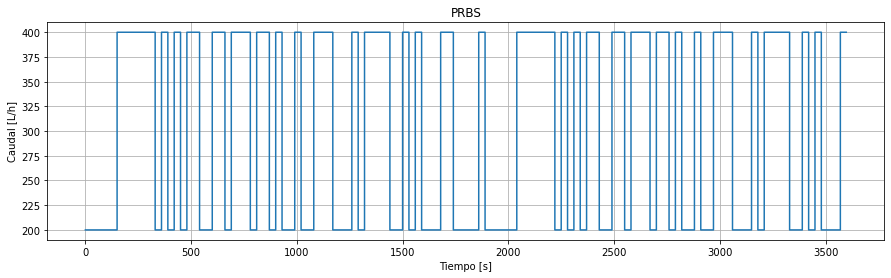
\includegraphics[width=0.75\linewidth]{PRBS.png}
    \caption{Ejemplo de señal PRBS con n=6.}
    \label{fig:PRBS}
\end{figure}



\begin{comment}
    
Sin embargo, en este mismo estudio\cite{KNUDSEN2017937}, se utiliza el control predictivo (MPC) como una fuente de señales de entrada al sistema, en vez de aplicar señales artificiales, de la siguiente forma:
\begin{itemize}

    \item Primero, se identifica un modelo inicial con datos históricos normales, donde no se requieren señales especiales.
    \item Luego, se usa este modelo para implementar un control predictivo durante 14 días. El MPC genera acciones de control que sirven como señal de entrada variada, las que tienen contenido frecuencial natural derivado de optimizar el consumo energético.
    \item Finalmente, se reidentifica el modelo térmico con esos nuevos datos generados por el MPC, teniendo una calidad comparable a uno obtenido con PRBS, pero sin incomodidad térmica ni experimentos intrusivos.
\end{itemize}
Eso funciona, ya que el MPC no solo controla el sistema, sino que, al reaccionar a restricciones térmicas, naturalmente excita al sistema, provocando variaciones suficientes en la calefacción, para que su comportamiento pueda ser modelado \cite{KNUDSEN2017937}.

\end{comment}





También se destacan las señales sinusoidales, ilustrada en la Figura \ref{fig:señal1}, como una alternativa ampliamente utilizada en experimentos de identificación \cite{Retzler2022}. Este tipo de señales permite excitar de manera controlada frecuencias específicas del sistema, lo que facilita la estimación de funciones de respuesta en frecuencia y el análisis de la relación entre la señal de entrada y la respuesta de salida\cite{ljung1999system}. En el caso de sistemas térmicos, esta característica resulta especialmente relevante, ya que la dinámica dominante suele concentrarse en bajas frecuencias, debido a la inercia térmica y a los procesos de almacenamiento y transferencia de energía. Por ello, el uso de señales sinusoidales permite estudiar de forma selectiva aquellas frecuencias donde se espera que el sistema entregue mayor información.

\begin{figure}[H]
    \centering
    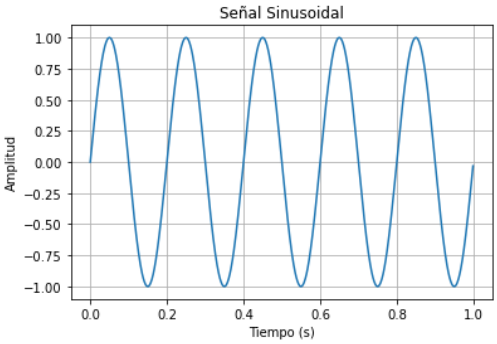
\includegraphics[width=0.5\linewidth]{señal sinusoidal.png}
    \caption{Señal sinusoidal en el dominio del tiempo.}
    \label{fig:señal1}
\end{figure}

No obstante, la aplicación de una señal sinusoidal pura permite excitar solo una frecuencia a la vez, por lo que una caracterización completa del sistema requiere realizar ensayos sucesivos con distintas frecuencias y amplitudes \cite{ljung1999system}. Esto puede aumentar considerablemente el tiempo experimental, especialmente en sistemas térmicos, donde cada condición de excitación debe mantenerse el tiempo suficiente para que la respuesta de temperatura sea observable. Por esta razón, el diseño de señales sinusoidales debe considerar cuidadosamente la selección de frecuencias, amplitudes y duración de los ensayos, evitando tanto excitaciones demasiado rápidas, que pueden ser filtradas por la inercia térmica, como amplitudes excesivas, que podrían llevar al sistema fuera de su rango normal de operación \cite{6842658}.


Una alternativa más eficiente corresponde al uso de señales multisinusoidales, las cuales se construyen como la suma de varias componentes sinusoidales de distintas frecuencias. 
Su expresión general puede escribirse como:
\begin{equation} \label{ecuacionmultiseno} 
u(t)=\sum\limits_{k=1}^{d} A_k cos(\omega_kt+\varphi_k)
\end{equation}
donde:
\begin{itemize}
    \item $A_k$: Amplitud de componente $k-$ésima.
    \item $\omega_k$: Frecuencia angular.
    \item $\varphi_k$: Fase.
\end{itemize}

A diferencia de una señal sinusoidal simple, una multisinusoide permite excitar simultáneamente un conjunto de frecuencias dentro de una banda de interés, reduciendo el tiempo requerido para obtener información dinámica del sistema. 
Para su diseño se deben definir los siguientes parámetros \cite{ljung1999system}:
\begin{enumerate}

%Es por ello que, de acuerdo con registros históricos y limitaciones instrumentales del sistema, en este trabajo se fijó en $T=2 $ segundos.
\item \textbf{Intervalo de muestreo ($T_s$)}: Define la discretización temporal de la señal y está determinado por el sistema de adquisición de datos, de manera análoga a la señal PRBS.
\item \textbf{Longitud máxima ($M$)}: El parámetro $M$ define el número de muestras por período de la señal multiseno y, junto al intervalo de muestreo, determina el período fundamental $T_0=MT_s$ y la resolución espectral $\Delta f=1/MT_s$. Para que la señal sea capaz de excitar las dinámicas más lentas del sistema, la resolución espectral debe ser comparable o menor a la frecuencia mínima de interés %($f_{min}=0.0005Hz$) 
, lo que conduce al criterio $M\gtrsim 1/(f_{min}T_s)$. 
%Con los valores considerados en este estudio, este criterio sugiere un $M$ aproximado de 1000 muestras por período. 
No obstante, Ljung formula los métodos de análisis en frecuencia bajo señales periódicas observadas en régimen estacionario, lo que implica que el análisis debe realizarse sobre un número entero de períodos. 
%Dado que la duración del experimento se fijó en 1 hora (3600 segundos), se seleccionó un $M$ igual a 900 muestras, lo que permite observar exactamente dos períodos completos en la ventana experimental. Esta elección mantiene una resolución espectral muy cercana a la frecuencia mínima de interés y garantiza la periodicidad de la señal en la ventana de análisis, evitando efectos de fija espectral.

%\item \textbf{Conjunto de frecuencias excitadas ($f_k$)}: Las frecuencias de la señal multisinuosidal se definen a partir de índices enteros $l_k$ asociados a la rejilla de la transformada discreta de Fourier, de modo que las componentes sinusoidales sean exactamente periódicas con período $M$. Las frecuencias físicas asociadas se obtienen como: $$f_k=l_k/(MT_s)$$

%En este trabajo, las frecuencias se seleccionaron de una banda de interés definida por $f_{min}$ y $f_{max}$, coherente con la dinámica térmica del sistema, evitando excitar frecuencias innecesarias o físicamente irrelevantes. 


\item \textbf{Fase ($\varphi_k$)}: Se introducen para reducir el factor de cresta de la señal, es decir, la relación entre el valor pico y el valor RMS. Una reducción del factor de cresta mejora la factibilidad experimental al disminuir el riesgo de saturaciones y esfuerzos excesivos sobre el actuador. Ljung \cite{ljung1999system} recomienda el uso de fases de Schroeder, las cuales permiten distribuir la energía de la señal de manera más uniforme en el tiempo, manteniendo el contenido espectral deseado. En la Figura \ref{fig:multiseno} se observa una señal multisinusoidal con fase de Schroeder.
\item \textbf{Número de componentes sinusoidales ($d$)}: Corresponde al número total de componentes sinusoidales incluidas en la señal y determina la densidad espectral dentro de la banda excitada. Un mayor valor de $d$ permite una representación más detallada del comportamiento en frecuencia del sistema, pero distribuye la energía entre más líneas espectrales, lo que puede afectar la relación señal-ruido.
%Siguiendo los criterios de Ljung, $d$ se seleccionó teniendo en cuenta la cobertura espectral suficiente y la factibilidad experimental,


%\item \textbf{Amplitud ($A_k$)}: Las amplitudes determinan la energía asignada a cada frecuencia excitada. Su selección debe equilibrar la necesidad de obtener una buena relación  señal-ruido con las limitaciones físicas del actuador. 
%En este estudio se utilizaron amplitudes uniformes para todas las componentes, lo que simplifica el diseño y asegura una excitación balanceada de la banda de interés. La señal se escaló a un rango físico de operación mediante un valor medio $u_0=300 L/h$ y una amplitud máxima de variación $\Delta u$, la se tomó igual a 50, 100 y 150 $L/h$ como se dijo anteriormente.

\item \textbf{Número de períodos ($K$)}: El parámetro $K$ define el número de períodos completos de la señal multisinusoidal incluidos en el experimento. 
%En este trabajo se utilizó $K=2$, lo que presenta una alineación adecuada entre calidad de estimación y duración total del experimento, especialmente considerando la dinámica lenta del sistema térmico.
\end{enumerate}

\begin{figure}[H]
    \centering
    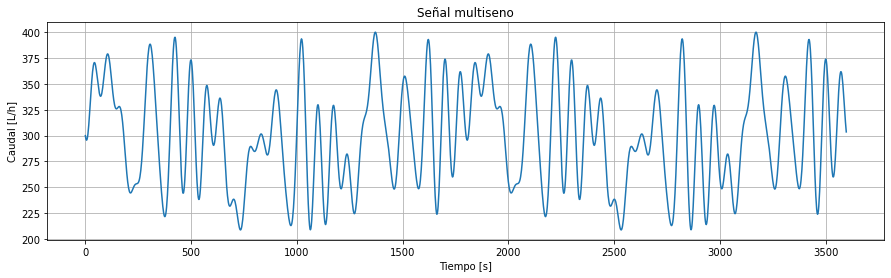
\includegraphics[width=0.75\linewidth]{Señal multiseno.png}
    \caption{Ejemplo de señal multisinusoidal con fase de Schroeder.}
    \label{fig:multiseno}
\end{figure}


Es posible abordar la optimización de señales multisinusoidales mediante la minimización del factor de cresta \cite{Retzler2022}, con el objetivo de reducir los valores máximos de la señal. Este aspecto es relevante en sistemas térmicos, ya que un bajo factor de cresta permite entregar energía de excitación de manera más uniforme, reduciendo la probabilidad de generar picos de potencia o caudal que puedan inducir comportamientos no lineales no deseados.

Además del bajo factor de cresta, las señales multisinusoidales presentan ventajas importantes para la identificación en el dominio de la frecuencia. Al ser señales periódicas y construidas con componentes frecuenciales conocidas, permiten controlar de forma precisa el contenido espectral de la excitación y reducir problemas asociados a la fuga espectral. Esto facilita la obtención de funciones de respuesta en frecuencia y permite analizar con mayor claridad la contribución de cada banda de frecuencia en la respuesta del sistema. En sistemas térmicos, esta propiedad es especialmente útil, ya que permite concentrar la energía de la señal en la banda de bajas frecuencias, donde se manifiestan principalmente las constantes de tiempo del proceso \cite{ljung1999system}.




Un aspecto relevante de las señales multisinusoidales es que también pueden emplearse para estudiar posibles efectos no lineales. De acuerdo con \cite{csurcsia2020user}, el uso de multisinusoides con estructuras específicas, por ejemplo excitando solo ciertos armónicos o introduciendo saltos aleatorios de armónicos, permite distinguir entre la respuesta lineal del sistema, el ruido y las distorsiones asociadas a no linealidades. Esto es importante en sistemas térmicos, ya que aunque muchas veces se modelan inicialmente como sistemas lineales alrededor de un punto de operación, pueden presentar comportamientos no lineales cuando varían las condiciones de caudal, potencia térmica o temperatura. Asimismo, aplicar distintos niveles de excitación permite evaluar si la dinámica del sistema cambia con la amplitud de la entrada, lo que constituye un indicio relevante de no linealidad.






































Además de las señales PRBS y multisinusoidales, existen otras formas de excitación que pueden utilizarse en identificación de sistemas. El diseño de una señal de entrada debe asegurar que el experimento sea suficientemente informativo, es decir, que la señal aplicada contenga la riqueza frecuencial necesaria para revelar la dinámica del sistema. Sin embargo, esta condición debe compatibilizarse con restricciones prácticas, tales como los límites de amplitud de los actuadores, la duración del experimento y la posibilidad de mantener el sistema dentro de un rango de operación seguro \cite{ljung1999system}. En sistemas térmicos, esta consideración es especialmente importante, ya que la inercia térmica atenúa las variaciones rápidas y concentra la información dinámica útil en bajas frecuencias.

En este contexto, además de la dos anteriores, Ghoreyshi et al. \cite{ghoreyshi2024design} analizan otras señales de excitación para la identificación aerodinámica de una aeronave genérica mediante simulaciones CFD. Aunque la aplicación corresponde a un sistema aerodinámico y no térmico, el estudio resulta útil desde el punto de vista metodológico, ya que compara diferentes señales diseñadas para excitar la dinámica del sistema y evaluar su capacidad para generar datos informativos:


\begin{itemize}
\item Señal chirp: Corresponde a un barrido de frecuencia continuo (Figura \ref{fig:chirp}) que comienza en una frecuencia baja y aumenta progresivamente, permitiendo excitar una amplia banda de frecuencias con una sola señal. Su amplitud se mantiene constante y su principal ventaja es la capacidad de explorar gradualmente el comportamiento del sistema en distintas frecuencias. Para un sistema térmico, una señal chirp puede ser útil siempre que el barrido se diseñe dentro de la banda de bajas frecuencias relevante, ya que un aumento demasiado rápido de la frecuencia puede generar componentes que serán fuertemente atenuadas por la inercia térmica y, por tanto, aportar poca información a la identificación del modelo \cite{ljung1999system}. 

\begin{figure}[H]
    \centering
    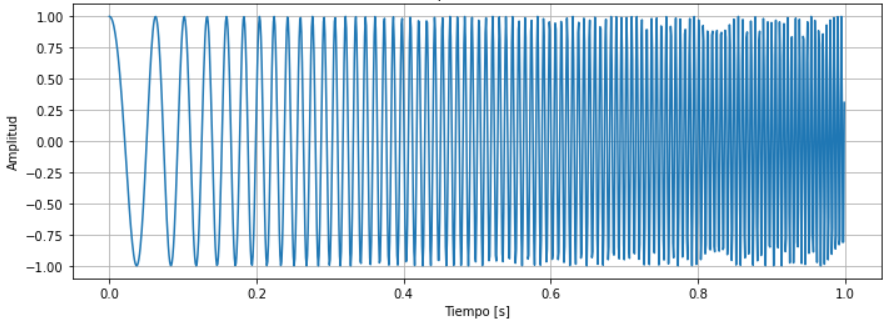
\includegraphics[width=0.5\linewidth]{señal chirp.png}
    \caption{Señal chirp.}
    \label{fig:chirp}
\end{figure}
    \item Señal gaussiana aleatoria: Corresponde a una excitación no estructurada, similar al ruido blanco, que puede distribuir energía en un rango amplio de frecuencias (Figura \ref{fig:señalgaussiana}). No obstante, presenta menor control directo sobre el contenido espectral y puede generar problemas de representatividad de los datos, especialmente si la energía no se concentra adecuadamente en la banda donde el sistema responde. En sistemas térmicos, esta limitación puede ser importante, ya que gran parte de la energía aplicada en frecuencias altas puede no producir variaciones observables en la temperatura.
    
    \begin{figure}[H]
        \centering
        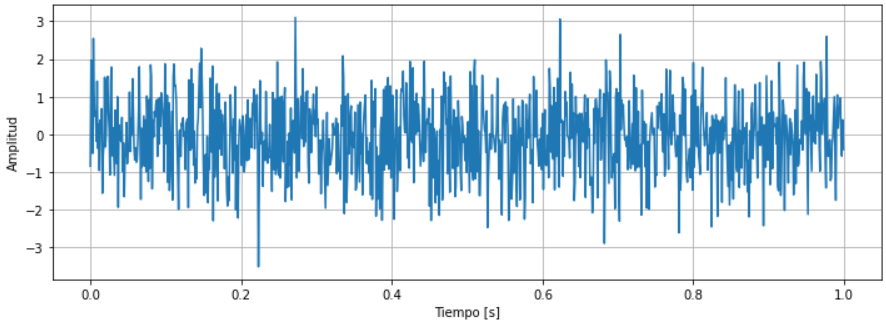
\includegraphics[width=0.5\linewidth]{señal gaussiana aleatoria.png}
        \caption{Señal gaussiana aleatoria.}
        \label{fig:señalgaussiana}
    \end{figure}
    \item Señal escalón: También es conocida como señal escalón unitaria y se utiliza habitualmente para estudiar la respuesta transitoria de un sistema. Se define como:

\[
u(t) = \left\{
\begin{array}{ll}
0, & \text{si } \quad    t < 0 \\
1, & \text{si }  \quad    t \geq 0
\end{array}
\right.
\]
En t$<$ 0, la señal está apagada. Vale 0.

En t$\geq0$ la señal se mantiene "encendida" con un valor constante, igual a 1.

En este caso, la entrada cambia bruscamente desde un valor inicial hasta un valor constante (Figura \ref{fig:escalon}). En sistemas térmicos, la señal escalón permite observar características como el retardo, el tiempo de subida, el tiempo de establecimiento y la ganancia térmica aproximada. Sin embargo, su capacidad para excitar un rango amplio de frecuencias es limitada en comparación con señales como PRBS o multisinusoidales.

    \begin{figure}[H]
        \centering
        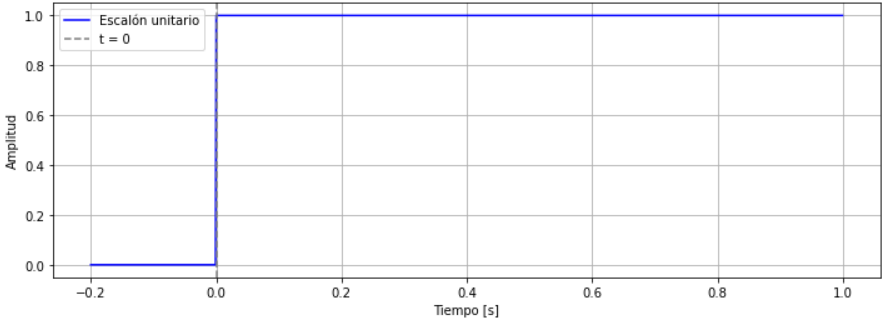
\includegraphics[width=0.5\linewidth]{señal escalon.png}
        \caption{Señal escalón.}
        \label{fig:escalon}
    \end{figure}
\end{itemize}

En el trabajo de Ghoreyshi et al. \cite{ghoreyshi2024design}, las señales fueron aplicadas en simulaciones bajo condiciones subsonoras, con un tiempo de muestreo de 0.0005 segundos y una duración de 4 segundos por prueba, precedida por un periodo breve de estabilización. Si bien estos valores son adecuados para el sistema aerodinámico estudiado, no son directamente transferibles a un sistema térmico, debido a que las escalas temporales son muy diferentes. En un banco térmico, el tiempo de muestreo, la duración total del experimento y la banda de excitación deben seleccionarse en función de las constantes de tiempo térmicas y de la frecuencia máxima que se desea identificar.

Los resultados reportados por Ghoreyshi et al. \cite{ghoreyshi2024design} indican que las señales multisinusoidales de Schroeder y las PRBS fueron las más efectivas para excitar el sistema y generar modelos precisos a partir de los datos simulados. En cambio, las señales gaussianas aleatorias y las señales escalón presentaron un desempeño inferior, ya sea por no excitar adecuadamente las frecuencias relevantes o por generar datos menos representativos del comportamiento dinámico. Esta conclusión es coherente con la identificación de sistemas térmicos, donde se requiere una señal suficientemente rica, pero al mismo tiempo compatible con la lentitud del proceso y las restricciones físicas del sistema.



En sistemas con múltiples entradas, como el sistema térmico estudiado, el diseño de señales de excitación resulta relevante. En este caso, las entradas pueden corresponder, por ejemplo, al caudal de trabajo y a la potencia térmica suministrada al sistema. Si ambas señales no se diseñan adecuadamente, puede producirse una alta correlación entre entradas, dificultando la identificación de la contribución individual de cada variable sobre la temperatura de salida. Por esta razón, para experimentos MISO o MIMO se recomienda utilizar señales suficientemente independientes entre sí. Esta condición permite mejorar la informatividad de los datos y reducir problemas de colinealidad en la identificación del modelo \cite{csurcsia2020user}.

En este contexto, la verificación previa y posterior de las señales de entrada resulta fundamental. No basta con generar señales con contenido frecuencial adecuado, también es necesario comprobar que los actuadores puedan reproducirlas correctamente, que las entradas no estén excesivamente correlacionadas y que la respuesta térmica presente variaciones medibles dentro de la banda de interés. Para el caso de un sistema térmico, esto implica analizar la energía espectral de las señales de caudal y potencia, la correlación entre ambas entradas, la coherencia entre entrada y salida y la posible presencia de distorsiones introducidas por los actuadores o por la propia dinámica térmica del banco experimental \cite{ljung1999system}.

%Otro concepto importante en el diseño experimental es la excitación persistente, la cual se refiere a la capacidad de una señal de entrada para contener suficiente riqueza dinámica como para identificar adecuadamente un modelo del sistema. Sin embargo, en procesos físicos reales y particularmente en sistemas térmicos, aplicar una única señal altamente excitante durante un tiempo prolongado puede resultar poco práctico, debido a la lentitud de la respuesta térmica, a las restricciones operativas y a la posibilidad de inducir condiciones no deseadas en los componentes. Por ello, Cao et al. \cite{cao2025informativity} proponen el concepto de excitación colectiva persistente, donde la información necesaria para la identificación no proviene necesariamente de una sola señal, sino del conjunto de varias señales o experimentos. Esta idea es especialmente pertinente para sistemas térmicos, ya que permite combinar diferentes ensayos, por ejemplo con PRBS, multisinusoides o variaciones operacionales, para cubrir de manera más completa la dinámica del sistema sin exigir una única prueba extensa o agresiva.

%Finalmente, además de asegurar que las señales sean suficientemente excitantes, es necesario considerar cómo los datos generados cubren el espacio de operación del sistema. En sistemas no lineales, la dinámica puede variar según el punto de operación, por ejemplo con el nivel de temperatura, el régimen de caudal o la potencia térmica aplicada. En este sentido, Herkersdorf y Nelles \cite{herkersdorf2025online} proponen una metodología basada en control por horizonte recedente para generar señales de entrada que distribuyan los datos de manera más uniforme dentro del espacio operativo del modelo. A diferencia de las señales clásicas, este enfoque no impone una forma fija de excitación, sino que construye la señal mediante un proceso de optimización orientado a explorar zonas poco representadas. Esta perspectiva resulta relevante para el sistema térmico estudiado, ya que permite entender que la calidad del modelo no depende únicamente del tipo de señal aplicada, sino también de que los datos experimentales representen adecuadamente las condiciones de operación bajo las cuales se espera utilizar el modelo.

En la Tabla \ref{tab:señales-excitacion} se presenta un resumen comparativo de las señales de entrada analizadas, considerando su cobertura espectral, factor de cresta, aplicaciones típicas y su facilidad de implementación. Esta comparación permite evaluar la pertinencia de cada señal para la identificación de sistemas térmicos, donde resulta fundamental excitar principalmente la dinámica de baja frecuencia, mantener las amplitudes dentro de rangos seguros de operación y obtener una respuesta de temperatura suficientemente observable.


\begin{table}[H]
\caption{Tabla comparativa de señales de excitación para identificación de sistemas dinámicos.}
\label{tab:señales-excitacion}
\centering
\resizebox{\textwidth}{!}{%
\begin{tabular}{|l|l|l|l|l|}
\hline
\textbf{Señal} & \textbf{Cobertura espectral} & \textbf{Factor de cresta} & \textbf{Aplicación típica} & \textbf{Implementación} \\ \hline

\textbf{PRBS} &
\begin{tabular}[c]{@{}l@{}}Amplia cobertura espectral.\\ Puede orientarse hacia bajas frecuencias.\end{tabular} &
\begin{tabular}[c]{@{}l@{}}Bajo.\\ Al ser binaria, mantiene amplitudes\\ acotadas y evita picos excesivos.\end{tabular} &
\begin{tabular}[c]{@{}l@{}}Identificación de sistemas dinámicos.\\ Adecuada para sistemas térmicos lentos,\\ excitando actuadores de tipo encendido/apagado.\end{tabular} &
\begin{tabular}[c]{@{}l@{}}Fácil de generar y aplicar.\\ Requiere definir amplitud, duración\\ y periodo de reloj.\end{tabular} \\ \hline

\textbf{\begin{tabular}[c]{@{}l@{}}Multi-\\ sinusoidal\end{tabular}} &
\begin{tabular}[c]{@{}l@{}}Controlada por las frecuencias\\ seleccionadas.\\ Permite concentrar energía en la\\ banda de interés.\end{tabular} &
\begin{tabular}[c]{@{}l@{}}Bajo a medio.\\ Puede reducirse mediante selección\\ adecuada de fases, como en señales\\ de Schroeder.\end{tabular} &
\begin{tabular}[c]{@{}l@{}}Identificación en el dominio de la\\ frecuencia.\\ Estimación de FRFs.\\ Análisis de posibles no linealidades.\end{tabular} &
\begin{tabular}[c]{@{}l@{}}Requiere definir frecuencias,\\ amplitudes, fases y número de periodos.\end{tabular} \\ \hline

\textbf{Chirp} &
\begin{tabular}[c]{@{}l@{}}Amplia cobertura mediante un\\ barrido progresivo de frecuencia.\\ Excita distintas frecuencias en una\\ sola prueba.\end{tabular} &
\begin{tabular}[c]{@{}l@{}}Medio. \\Generalmente mantiene amplitud\\ constante, aunque depende del diseño\\ del barrido.\end{tabular} &
\begin{tabular}[c]{@{}l@{}}Caracterización dinámica en un rango\\ de frecuencias.\end{tabular} &
\begin{tabular}[c]{@{}l@{}}Fácil de generar.\\ Requiere seleccionar frecuencia inicial,\\ frecuencia final y duración del barrido.\end{tabular} \\ \hline

\textbf{\begin{tabular}[c]{@{}l@{}}Gaussiana\\ aleatoria\end{tabular}} &
\begin{tabular}[c]{@{}l@{}}Amplia, pero poco controlada.\\ Puede distribuir energía en frecuencias\\ poco relevantes para sistemas térmicos.\end{tabular} &
\begin{tabular}[c]{@{}l@{}}Medio a alto.\\ Puede presentar picos aleatorios\\ dependiendo de la varianza de la señal.\end{tabular} &
\begin{tabular}[c]{@{}l@{}}Excitación general de sistemas dinámicos.\\ Puede requerir filtrado para concentrar\\ la energía en la banda de interés.\end{tabular} &
\begin{tabular}[c]{@{}l@{}}Es fácil de generar, pero requiere\\ limitar amplitudes, filtrar componentes\\ no deseadas y verificar seguridad\\ operacional.\end{tabular} \\ \hline

\textbf{Escalón} &
\begin{tabular}[c]{@{}l@{}}Limitada para identificación en\\ frecuencia.\\ Excita principalmente la respuesta\\ transitoria del sistema.\end{tabular} &
\begin{tabular}[c]{@{}l@{}}Bajo.\\ La señal cambia una vez y luego\\ permanece constante.\end{tabular} &
\begin{tabular}[c]{@{}l@{}}Estimación de retardo, ganancia,\\ tiempo de subida y tiempo de\\ establecimiento.\end{tabular} &
\begin{tabular}[c]{@{}l@{}}Es la señal más simple de aplicar.\\ Puede ser insuficiente para identificar\\ modelos dinámicos complejos.\end{tabular} \\ \hline



\end{tabular}%
}
\end{table}


A partir de lo anterior, las señales PRBS y multisinusoidales presentan características especialmente adecuadas para la identificación del sistema térmico en estudio. Ambas permiten excitar un rango amplio de frecuencias y generar variaciones suficientemente informativas para caracterizar la dinámica del banco de ensayos. A diferencia de señales aleatorias no estructuradas, como las señales gaussianas, estas alternativas permiten un mayor control sobre la amplitud y el contenido espectral de la excitación, lo que facilita su adaptación a las restricciones físicas y dinámicas del sistema.

En el caso de las señales PRBS, una de sus principales ventajas radica en la posibilidad de generar una excitación con contenido energético distribuido en una banda de frecuencias mediante una señal binaria y de implementación experimental relativamente sencilla. Esta característica resulta especialmente conveniente para actuar sobre variables que admiten estados discretos, como el aporte de potencia térmica mediante condiciones de encendido y apagado. Además, mediante el ajuste del periodo de reloj es posible adaptar la excitación a la dinámica lenta característica de los procesos térmicos, favoreciendo la concentración de información en bajas frecuencias y evitando variaciones excesivamente rápidas que podrían ser atenuadas por la inercia propia del sistema.

Por otra parte, las señales multisinusoidales permiten definir explícitamente las frecuencias que serán excitadas, lo que resulta particularmente útil cuando se desea concentrar la energía de entrada dentro de una banda de interés previamente establecida. Esta propiedad es relevante en sistemas térmicos, donde la dinámica dominante suele encontrarse asociada a componentes de baja frecuencia. Asimismo, mediante una selección adecuada de amplitudes y fases es posible reducir el factor de cresta de la señal, permitiendo introducir una excitación suficientemente energética sin generar valores máximos excesivos que puedan comprometer las condiciones de operación del banco de ensayos.

Estas características explican que tanto las secuencias binarias pseudoaleatorias como las señales multisinusoidales se encuentren ampliamente estudiadas y utilizadas en procedimientos de identificación de sistemas, tanto en aplicaciones académicas como industriales \cite{DRGONA2020190}, \cite{6842658}, \cite{aerospace12020074}, \cite{csurcsia2020user}, \cite{1655392}. En términos generales, las señales PRBS proporcionan una excitación de banda relativamente amplia, cuyo contenido frecuencial depende de sus parámetros de diseño, mientras que las señales multisinusoidales permiten distribuir de manera selectiva la energía de excitación en frecuencias previamente determinadas.

En este sentido, ambas alternativas pueden considerarse complementarias para el diseño de ensayos de identificación. La elección y parametrización de una señal de excitación no deben realizarse de manera arbitraria, sino considerando las características dinámicas del proceso, las restricciones operacionales del sistema, la amplitud admisible de las entradas y el intervalo de frecuencias en el cual se concentra la información relevante para la identificación \cite{ljung1999system}. Estos criterios adquieren especial importancia en sistemas térmicos, cuya respuesta se encuentra condicionada por fenómenos de acumulación energética, inercia térmica y retardos asociados al transporte del fluido.

Adicionalmente, en configuraciones de múltiples entradas y una salida (MISO), el diseño de las señales debe permitir excitar simultáneamente las distintas variables de entrada, procurando que cada una aporte información suficiente sobre la respuesta del sistema y evitando, en lo posible, una elevada dependencia o correlación entre ellas.

En consecuencia, a partir de la revisión del estado del arte y de las características particulares del banco experimental, se establece el uso de señales PRBS y multisinusoidales como alternativas de excitación para el desarrollo de los ensayos de identificación. Su selección se fundamenta en la capacidad de ambas señales para excitar la dinámica relevante del proceso, proporcionar datos suficientemente informativos y mantener control sobre la amplitud y el contenido frecuencial de las entradas. Asimismo, sus propiedades permiten adaptar la excitación a la dinámica lenta del sistema y resultan compatibles con las restricciones físicas y operacionales del montaje experimental.

%De este modo, ambas señales serán diseñadas y evaluadas posteriormente bajo configuraciones SISO y MISO, analizando su capacidad para producir registros adecuados para la identificación del sistema. La comparación de su comportamiento experimental permitirá seleccionar las condiciones de excitación que proporcionen una representación más informativa de la relación entre el caudal, la potencia térmica y la temperatura de salida, estableciendo así la base experimental para el posterior desarrollo y validación de los modelos computacionales considerados en este trabajo.


%El diseño de experimentos evalúa qué excitaciones proporcionan los datos más útiles. Cuando el objetivo es construir un modelo adecuado para el control, las entradas generadas no necesitan cubrir todo el dominio de frecuencia, sino más bien una selección relevante para el control. Por lo tanto, el tiempo de muestreo debe elegirse en función de las constantes de tiempo del edificio, con un rango típico para sistemas de edificios entre 5 min y 60 min. En la identificación de sistemas de edificios, generalmente se utilizan señales binarias pseudoaleatorias (PRBS) y señales de operación normal (business as usual) para generar los conjuntos de datos de entrenamiento. La primera es probablemente la señal más apropiada para proporcionar datos enriquecidos ( Ljung, 1999 ), mientras que la segunda se utiliza para evitar los costos adicionales de los experimentos, así como los riesgos de incomodidad y la necesidad de soporte técnico. Los estudios de caso de identificación de sistemas de construcción usando PRBS como señales de entrada son ( Bacher, Madsen, 2011 , Hazyuk, Ghiaus, Penhouet, 2012 , Madsen, Holst, 1995 , Prívara, Váňa, Gyalistras, Cigler, Sagerschnig, Morari, Ferkl, 2011 , Royer, Thil, Talbert, Polit, 2014 ), mientras que los ejemplos de casos que usaron operación normal son ( Berthou, Stabat, Salvazet, Marchio, 2014 , Ferkl, Široký, 2010 , Reynders, Diriken, Saelens, 2014 , Verhelst ) \cite{DRGONA2020190}.

\section{Criterios espectrales para la evaluación de las señales generadas}
Para evaluar la calidad informativa de las señales generadas y de los datos adquiridos, se emplean criterios espectrales aplicables tanto a configuraciones con una sola entrada como a configuraciones con múltiples entradas. 
%En los ensayos SISO se consideró como entrada manipulada el caudal de agua y como salida la temperatura medida a la salida del sistema. En los ensayos MISO, en cambio, se consideraron dos entradas manipuladas: el caudal de agua y la potencia térmica suministrada mediante las resistencias eléctricas, manteniendo como salida la temperatura del fluido en el último colector.

El análisis espectral previo a la identificación de modelos permite verificar si las señales de entrada excitan adecuadamente la dinámica relevante del sistema y si existe una relación significativa entre las entradas manipuladas y la salida medida en el dominio de la frecuencia. En particular, se analizaron la densidad espectral de las señales, la coherencia entre entradas y salida, la función de respuesta en frecuencia y, en el caso MISO, la relación entre las propias señales de entrada. Este tipo de análisis constituye una herramienta fundamental para determinar si un conjunto de datos posee suficiente contenido informativo para la identificación de modelos dinámicos, además de permitir comparar distintos ensayos realizados bajo diferentes configuraciones de excitación \cite{ljung1999system}.

%\subsubsection{Potencia espectral}
%La potencia espectral de la señal de entrada se utiliza para verificar que la señal excite adecuadamente la banda de frecuencias de interés del sistema. Este análisis perimi



\subsubsection{Densidad espectral ($\Phi_x(\omega)$) }

La densidad espectral permite describir cómo se distribuye la energía o varianza de una señal en el dominio de la frecuencia. Para una señal discreta $x(k)$, la densidad espectral se define como la transformada de Fourier de su función de autocorrelación \cite{ljung1999system}:
\begin{equation} \label{densidadespectral} 
\Phi_x(\omega)=\sum\limits_{\tau=-\infty}^{\infty} R_x(\tau)e^{-j\omega\tau} 
\end{equation}
 donde:
 \begin{itemize}
     \item $R_x(\tau)$ es la función de autocorrelación de la señal $x(k)$.
 \end{itemize}

Esta magnitud permite identificar qué componentes frecuenciales concentran mayor energía y, por lo tanto, qué bandas de frecuencia son efectivamente excitadas por la señal. En el contexto de la identificación de sistemas, también se le denomina densidad espectral de potencia, ya que su integral sobre el dominio frecuencial está directamente relacionada con la varianza de la señal:
\begin{equation} \label{varianza} 
\text{var}(x) = \frac{1}{2\pi} \int_{-\pi}^{\pi} \Phi_x(\omega) \, d\omega
\end{equation}
Desde el punto de vista del diseño de señales de entrada, este criterio permite verificar si la excitación aplicada contiene energía suficiente en la banda de frecuencias donde se espera que el sistema presente su dinámica relevante. En el caso SISO, este análisis se aplica al caudal. En el caso MISO, se aplica tanto al caudal como a la potencia eléctrica, con el objetivo de comprobar que ambas entradas aporten información en la banda de interés. Si la densidad espectral de una entrada es muy baja o prácticamente nula en determinadas frecuencias, la respuesta del sistema en dichas bandas no podrá ser identificada adecuadamente a partir de los datos adquiridos.

Asimismo, la densidad espectral de la salida permite analizar en qué rango de frecuencias se concentra la respuesta térmica del sistema. En sistemas térmicos, esta información resulta especialmente relevante, ya que la mayor parte de la dinámica suele concentrarse en bajas frecuencias. Por esta razón, comparar la densidad espectral de las entradas con la densidad espectral de la salida permite verificar si las señales aplicadas son coherentes con la naturaleza dinámica del proceso.

En el gráfico ilustrativo de densidad espectral de potencia (Figura \ref{fig:EJEMPLOdensidadespectral}) se observa la distribución de energía de las señales de entrada y salida en función de la frecuencia. Este tipo de gráfico permite verificar si las señales aplicadas entregan excitación suficiente en el rango frecuencial relevante. Si la densidad espectral de una entrada es muy baja en una determinada banda, la respuesta del sistema en esas frecuencias no podrá ser identificada con suficiente confiabilidad. También es importante considerar que no toda la información del gráfico tiene la misma relevancia. En este estudio, la interpretación debe concentrarse principalmente en la banda de interés del sistema térmico. Fuera de ese rango, la energía puede ser menor, estar asociada a ruido o no aportar información relevante para la identificación del modelo.
\begin{figure}[H]
    \centering
    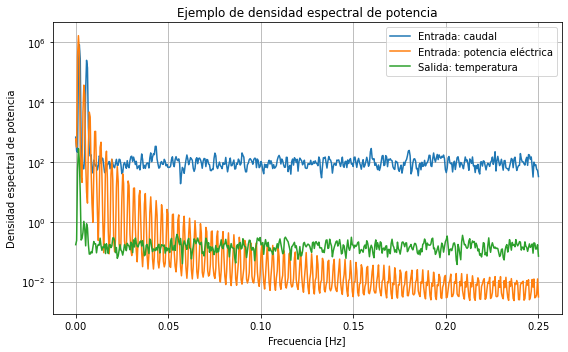
\includegraphics[width=0.5\linewidth]{Figure 2026-07-05 201123 (0).png}
    \caption{Ejemplo ilustrativo de gráfico de densidad espectral.}
    \label{fig:EJEMPLOdensidadespectral}
\end{figure}


%También, para dos señales discretas $x(k)$ e $y(k)$ se define la densidad espectral cruzada como:
%$$\Phi_{xy}(\omega)=\sum\limits_{\tau=-\infty}^{\infty} R_{xy}(\tau)e^{-j\omega\tau} $$
%Donde:
% \begin{itemize}
 %    \item $R_{xy}(\tau)$ representa la correlación cruzada entre $x(k)$ e $y(k)$.
% \end{itemize}

%La densidad espectral cruzada es una función compleja que describe la relación estadística entre ambas señales en el dominio de la frecuencia. Mide la intensidad de la relación entre $x$ e $y$ a cada frecuencia, el desfase entre las componentes frecuenciales y qué parte de las señales está correlacionada. Esta magnitud permite identificar qué parte del comportamiento de la salida está correlacionada con la entrada y en qué bandas de frecuencia dicha correlación es significativa.


\subsubsection{Coherencia($\gamma^2(\omega)$)}

La coherencia espectral es una medida normalizada de la dependencia lineal entre dos señales en el dominio de la frecuencia. Se define como:
\begin{equation} \label{coherencia} 
\gamma^2(\omega)=\frac{|\Phi_{xy}(\omega)|^2}{\Phi_{x}(\omega)\Phi_{y}(\omega)}
\end{equation}
Esta magnitud está acotada entre 0 y 1, y puede interpretarse como la fracción de la densidad espectral de una señal que puede ser explicada linealmente a partir de otra señal en cada frecuencia.

En los ensayos SISO, la coherencia entre caudal y temperatura permite evaluar si la salida térmica está relacionada de manera significativa con la entrada aplicada. Una coherencia cercana a 1 indica que la respuesta de la temperatura puede ser explicada en gran medida por las variaciones del caudal en esa frecuencia, lo que favorece la identificación de un modelo dinámico lineal. En cambio, una coherencia baja puede indicar presencia de ruido, perturbaciones no medidas, baja energía de excitación o posibles efectos no lineales.
En los ensayos MISO, la coherencia debe analizarse entre cada entrada y la salida. De esta forma, se evalúa separadamente la relación entre el caudal y la temperatura, y entre la potencia eléctrica y la temperatura. Este análisis permite determinar si ambas entradas aportan información útil para explicar la respuesta térmica del sistema. Una coherencia alta entre una entrada y la salida sugiere que dicha entrada tiene una influencia significativa sobre la temperatura en la banda de frecuencia analizada. Por el contrario, una coherencia baja puede indicar que la entrada no excita suficientemente al sistema, que su efecto queda enmascarado por otra variable o que existen perturbaciones no consideradas. Además, se espera que la coherencia entre las entradas sea baja o moderada, de manera que entreguen información diferenciable al proceso de identificación.

En el gráfico ilustrativo de coherencia espectral (Figura \ref{fig:Ejemlpocoherencia}) se muestran las relaciones entre cada entrada y la salida, además de la coherencia entre las dos entradas. En una situación favorable para la identificación MISO, las curvas de coherencia entrada-salida deberían presentar valores relativamente altos en la banda de interés, mientras que la coherencia entre entradas debería mantenerse baja. Esto permite inferir que cada señal de entrada contribuye de forma independiente a explicar la temperatura de salida.
\begin{figure}[H]
    \centering
    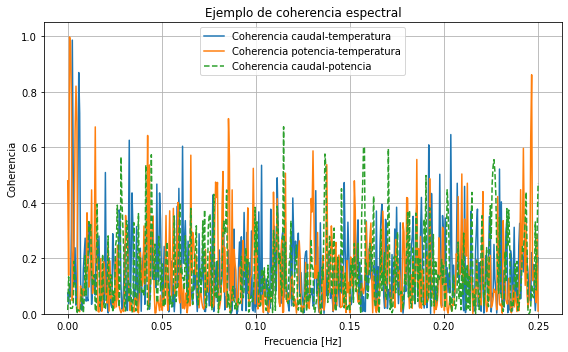
\includegraphics[width=0.5\linewidth]{Figure 2026-07-05 201123 (1).png}
    \caption{Ejemplo ilustrativo de coherencia espectral.}
    \label{fig:Ejemlpocoherencia}
\end{figure}
\subsubsection{Función de respuesta en frecuencia (FRF)}

La función de respuesta en frecuencia (FRF) es una representación no paramétrica que permite describir la relación dinámica entre una señal de entrada y una señal de salida en el dominio de la frecuencia. Esta función indica cómo un sistema modifica las distintas componentes frecuenciales de la entrada, entregando información tanto sobre la ganancia como sobre el desfase introducido por la dinámica del proceso. En otras palabras, la FRF permite analizar de qué manera el sistema amplifica, atenúa o retrasa la respuesta frente a excitaciones de distinta frecuencia.
La estimación de la respuesta frecuencial puede realizarse a partir de métodos no paramétricos en el dominio de la frecuencia. En particular, una forma ampliamente utilizada consiste en estimar la FRF mediante análisis espectral, a partir del cociente entre la densidad espectral cruzada de salida–entrada y la densidad espectral de potencia de la entrada \cite{ljung1999system}:
\begin{equation} \label{frf} 
\hat{G(e}^{j\omega})=\frac{\Phi_{yu}(\omega)}{\Phi_{u}(\omega)}
\end{equation}
Esta expresión permite obtener una estimación suavizada de la respuesta en frecuencia a partir de datos medidos, lo que resulta especialmente útil cuando se trabaja con señales experimentales afectadas por ruido.

La FRF es una función compleja, por lo que su interpretación se realiza habitualmente mediante dos representaciones complementarias: la magnitud y la fase. La magnitud muestra cuánto amplifica o atenúa el sistema cada componente frecuencial de la entrada, mientras que la fase representa el desfase entre entrada y salida introducido por la dinámica del sistema. Por lo tanto, ambas curvas no corresponden a estimaciones distintas, sino a dos formas de representar la misma función de respuesta en frecuencia.

En el gráfico de magnitud de la FRF (Figura \ref{fig:EjemploFRFmagnitud}) se observa cómo varía la ganancia del sistema en función de la frecuencia. De manera general, este tipo de gráfico permite identificar los rangos frecuenciales en los que la salida responde con mayor o menor intensidad frente a la excitación aplicada. Cuando la magnitud disminuye al aumentar la frecuencia, ello indica que el sistema atenúa las variaciones rápidas y responde preferentemente a componentes lentas, comportamiento característico de sistemas con dinámica dominante en bajas frecuencias. Por su parte, el gráfico de fase (Figura \ref{fig:EjemploFRFfase} muestra el desfase entre la entrada y la salida para cada frecuencia analizada. Este gráfico permite evaluar el efecto de retardos, almacenamiento de energía e inercia dinámica presentes en el sistema. En términos generales, una variación progresiva de la fase con la frecuencia refleja que la respuesta no ocurre de manera instantánea, sino que existe un desfase asociado al comportamiento dinámico del proceso.

\begin{figure}[H]
    \centering
    % Subfigura 1: Magnitud
    \begin{subfigure}{0.48\linewidth}
        \centering
        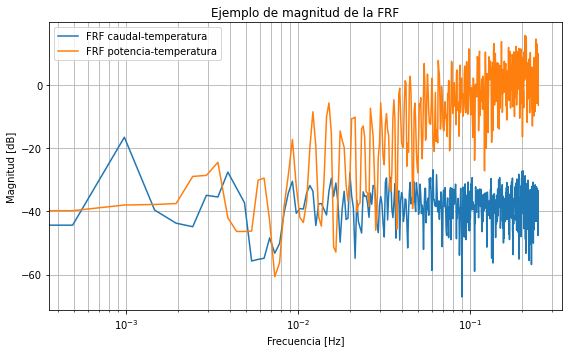
\includegraphics[width=\linewidth]{Figure 2026-07-05 201123 (2).png}
        \caption{Magnitud de la FRF.}
        \label{fig:EjemploFRFmagnitud}
    \end{subfigure}
    \hfill % Rellena el espacio horizontal entre ambas
    % Subfigura 2: Fase
    \begin{subfigure}{0.48\linewidth}
        \centering
        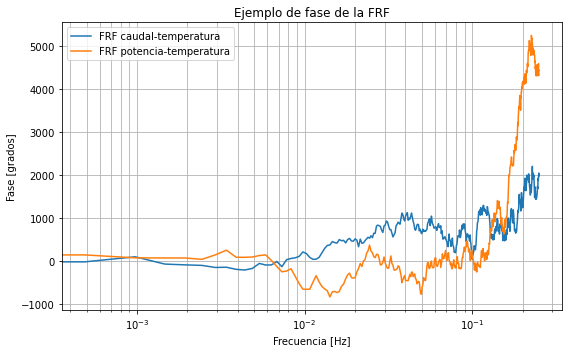
\includegraphics[width=\linewidth]{Figure 2026-07-05 201123 (3).png}
        \caption{Fase de la FRF.}
        \label{fig:EjemploFRFfase}
    \end{subfigure}
    
    \caption{Ejemplo ilustrativo de la función de respuesta en frecuencia (FRF).}
    \label{fig:FRF_completa}
\end{figure}
En el contexto del sistema en estudio, la FRF se utiliza como una herramienta para evaluar si las señales aplicadas excitan adecuadamente la dinámica relevante del proceso y para analizar la consistencia de la relación dinámica entre las variables manipuladas y la salida medida. De este modo, la magnitud y la fase de la FRF complementan el análisis realizado mediante la densidad espectral de potencia y la coherencia, aportando una representación más completa del comportamiento dinámico del sistema en el dominio de la frecuencia.
\subsubsection{Independencia entre señales de entrada}

En ensayos con más de una entrada o MISO, además de evaluar la relación entre cada entrada y la salida, es necesario analizar la independencia relativa entre las señales manipuladas. Este criterio es importante porque, si presentan una dependencia elevada entre sí, el proceso de identificación puede tener dificultades para distinguir qué parte de la respuesta se debe a cada entrada.

Para evaluar esta condición se puede utilizar la correlación cruzada en el dominio temporal y la coherencia entre entradas en el dominio de la frecuencia. Una baja correlación entre caudal y potencia eléctrica indica que ambas señales varían de manera suficientemente diferenciada durante el ensayo. Esto favorece la estimación de modelos MISO, ya que reduce problemas de colinealidad y permite separar de mejor manera la contribución de cada entrada sobre la temperatura.

En el análisis posterior de los datos se debe observar que la correlación cruzada entre las entradas sea reducida para la mayoría de los retardos evaluados. En particular, valores máximos de correlación alejados de 1 en valor absoluto indican que no existe una relación temporal dominante entre ambas señales. Se utiliza un límite máximo de correlación de 0.8 \cite{csurcsia2020user}. De forma complementaria, una baja coherencia entre caudal y potencia eléctrica dentro de la banda de interés refuerza la idea de que las entradas son suficientemente independientes.

En el gráfico ilustrativo de correlación cruzada entre entradas (Figura \ref{fig:EJEMPLOcorrelacion}) se observa una señal con valores bajos de correlación normalizada. Este comportamiento es deseable en una configuración MISO, ya que sugiere que las entradas no se encuentran fuertemente relacionadas entre sí. Por lo tanto, cada variable manipulada puede aportar información propia al proceso de identificación del modelo.
\begin{figure}[H]
    \centering
    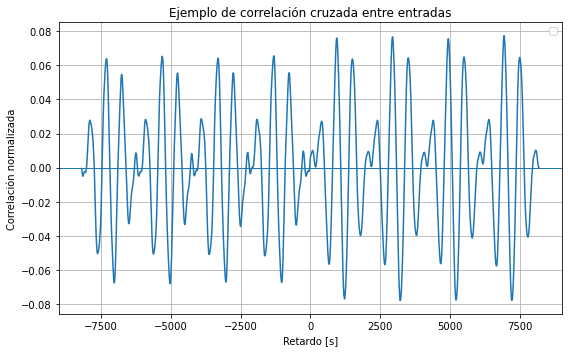
\includegraphics[width=0.5\linewidth]{Figure 2026-07-05 201123 (4).png}
    \caption{Ejemplo ilustrativo de correlación.}
    \label{fig:EJEMPLOcorrelacion}
\end{figure}














































\chapter{Caracterización, modelado y validación del sistema} 

\section{Descripción del sistema}

El banco de pruebas experimental utilizado en este trabajo corresponde a un sistema térmico de emulación termosolar a escala reducida (Figura \ref{fig:placeholdesdsfdsf}), diseñado con el objetivo de reproducir el comportamiento térmico del receptor de una planta termosolar real bajo condiciones controladas de laboratorio. 


\begin{figure}[H]
    \centering
    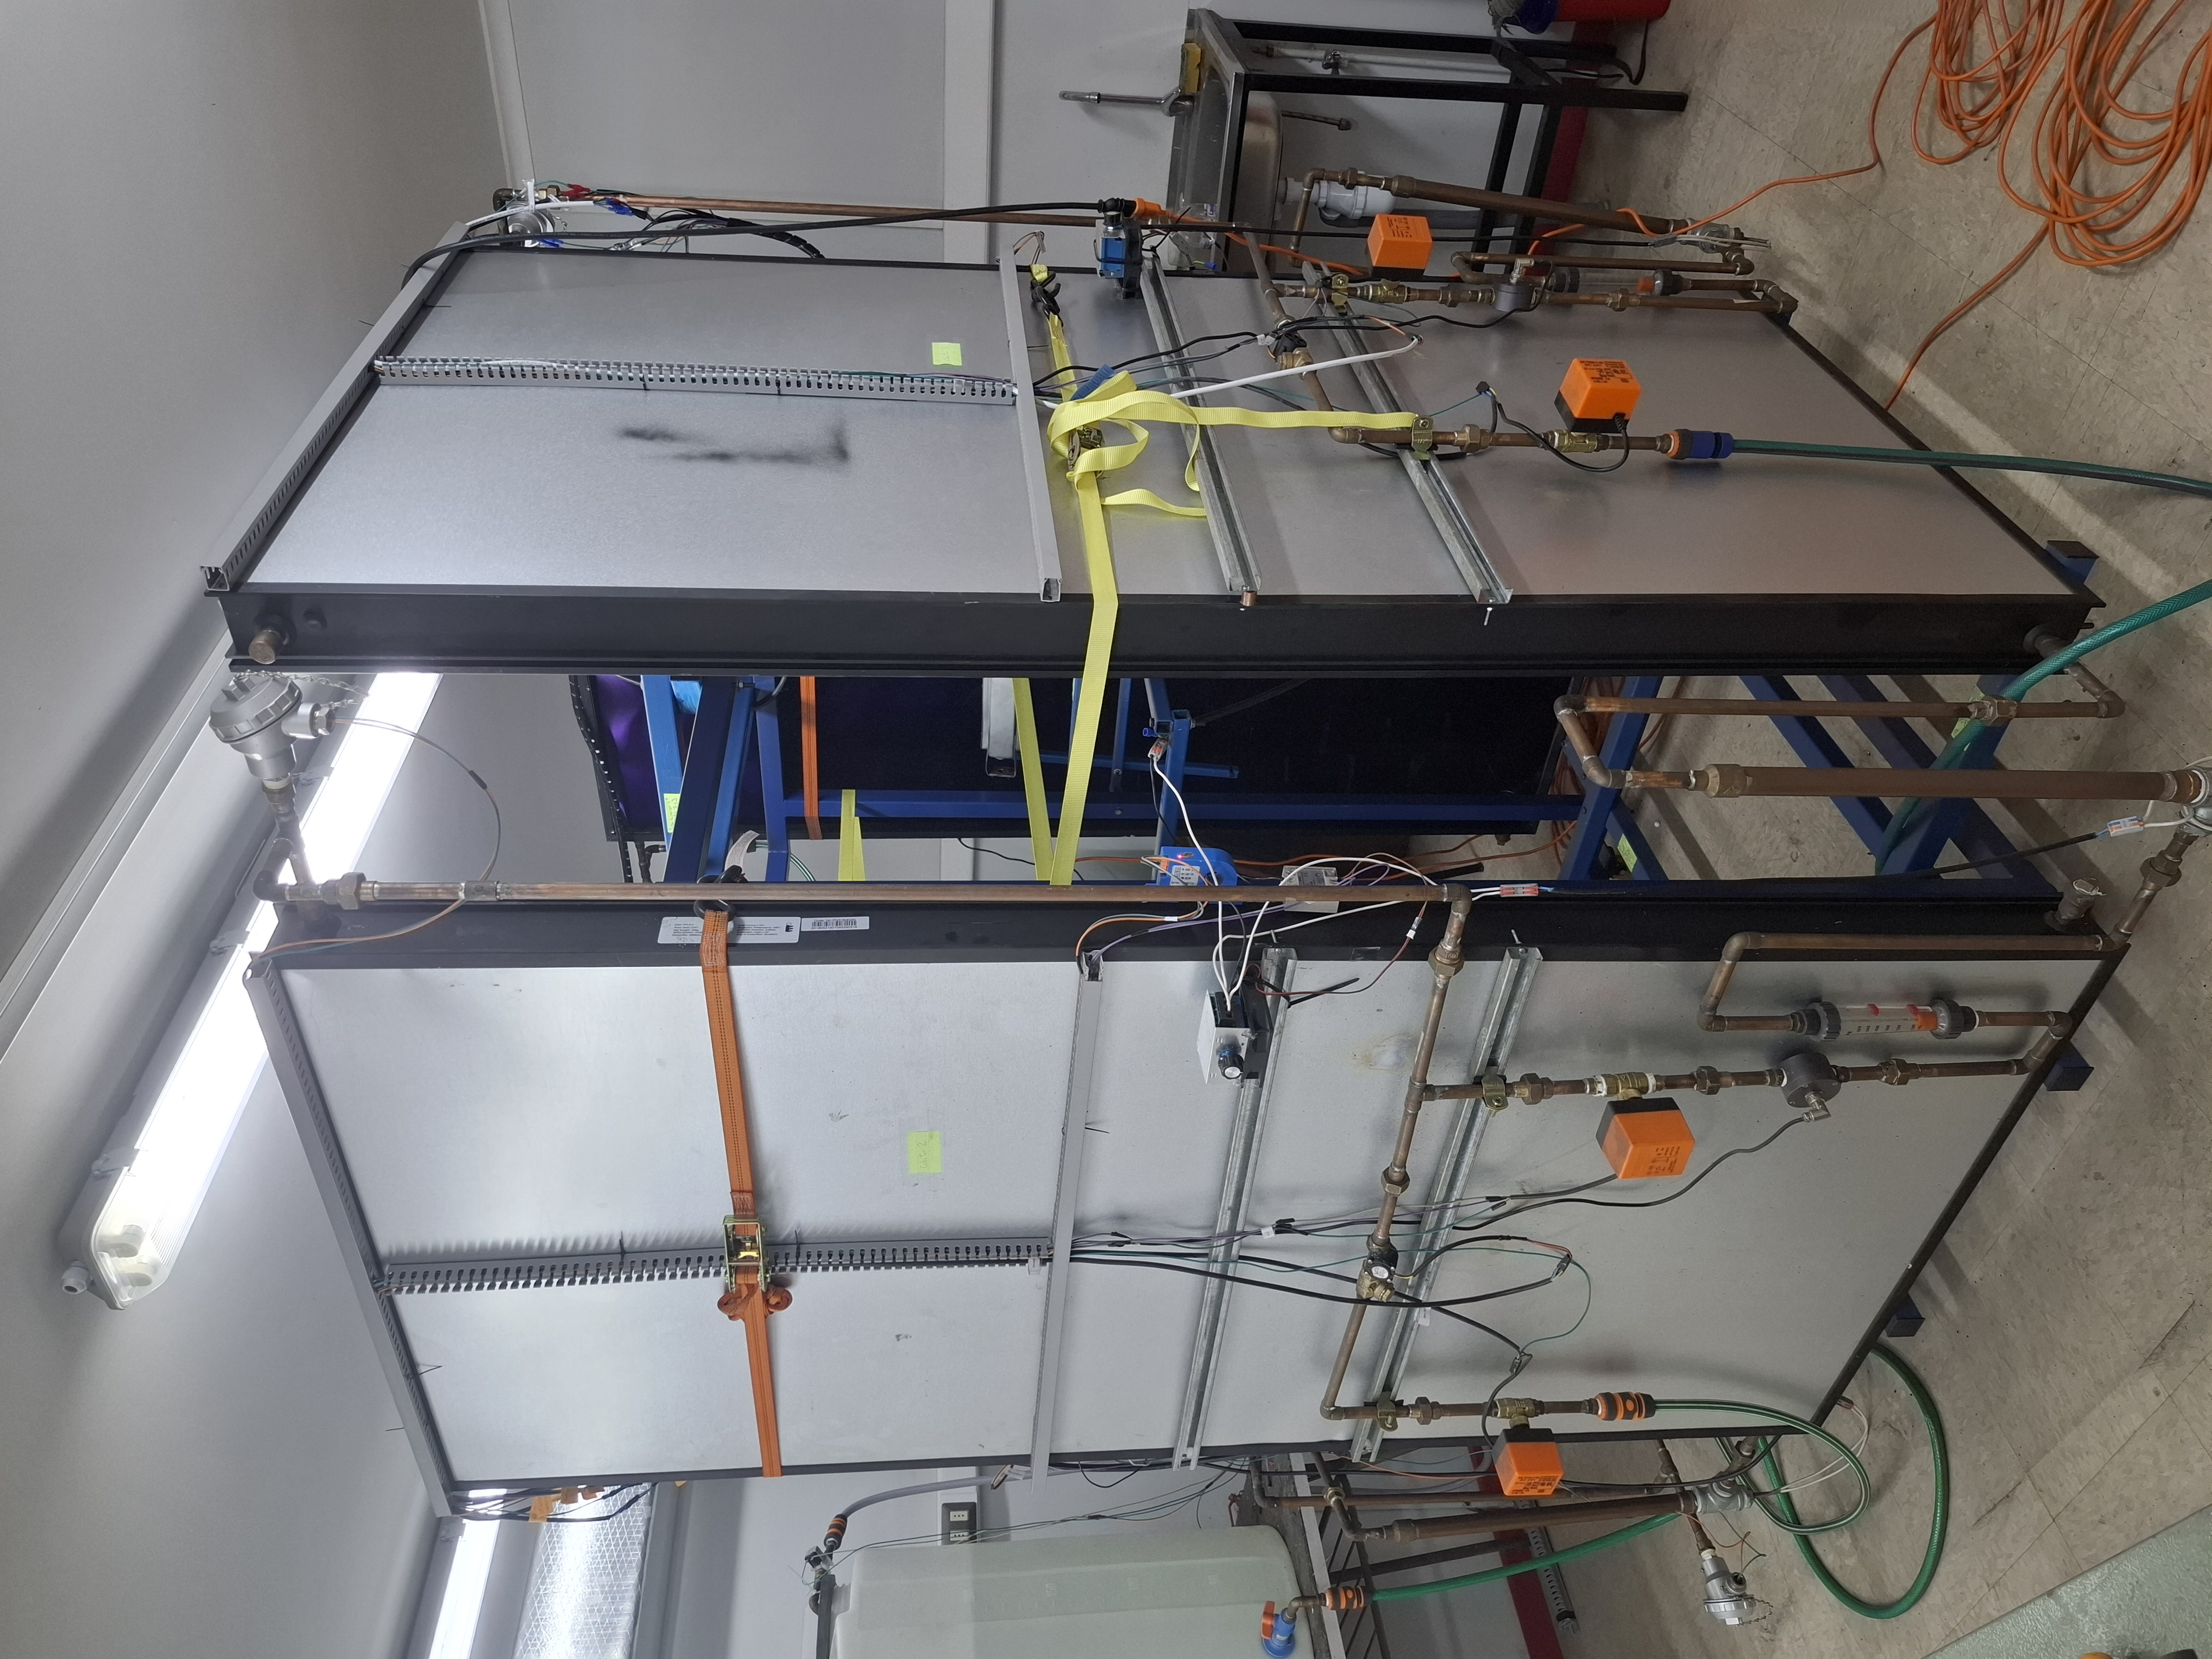
\includegraphics[width=0.45\linewidth, angle=-90]{banco de ensayo.jpg}
    \caption{Banco de pruebas.}
    \label{fig:placeholdesdsfdsf}
   
\end{figure}


El receptor en una planta termosolar, constituye el elemento encargado de absorber la energía térmica proveniente de la radiación solar concentrada y transferirla al fluido de trabajo. Dependiendo de la tecnología empleada, como torre central, colectores cilindro-parabólicos o Fresnel lineal, el receptor puede adoptar distintas configuraciones geométricas y constructivas, aunque su principio de operación es común. La trayectoria que recorre el fluido dentro del receptor puede ser variable. En la Figura \ref{fig:receptor} se muestra un ejemplo representativo, cuya disposición resulta análoga a la implementada en el sistema termosolar analizado en este trabajo.


\begin{figure}[H]
    \centering
    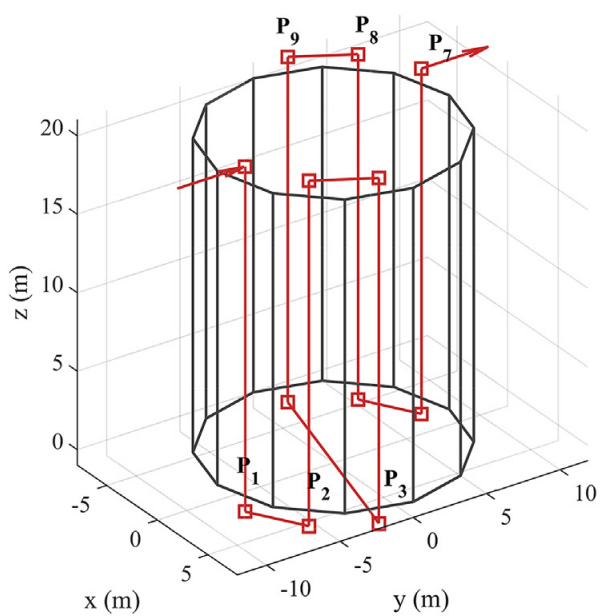
\includegraphics[width=0.5\linewidth]{Screenshot_2.png}
    \caption{Ilustración de receptor central y la trayectoria del fluido \cite{GARCIA20221221}.}
    \label{fig:receptor}
\end{figure}
%\begin{figure}[H]
  %  \centering
   % 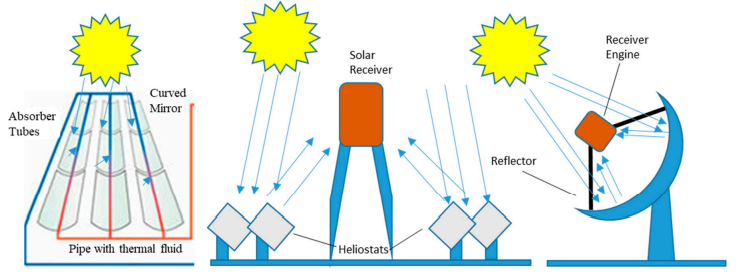
\includegraphics[width=0.65\linewidth]{tipos de tecnologias de concetracion.png}
   % \caption{Principales configuraciones del receptor de los sistemas de energía solar concentrada \cite{en12163079}.}
   % \label{fig:tecnologias}
%\end{figure}


Desde un punto de vista funcional, el banco experimental reproduce los principios fundamentales de operación de un sistema termosolar a escala real, en particular del receptor térmico de una planta. En ambos casos, un fluido de transferencia de calor circula a través de un conjunto de elementos de intercambio térmico, acumulando energía térmica a lo largo de su recorrido, mientras el caudal actúa como una variable clave para el control de la temperatura de salida.

Si bien el banco experimental no replica el mecanismo de captación de energía solar ni las pérdidas térmicas ambientales propias de un receptor a escala real, sí conserva los aspectos dinámicos esenciales asociados al transporte de energía, la acumulación térmica y el acoplamiento entre variables hidráulicas y térmicas. Esta similitud funcional justifica su utilización como plataforma experimental para el análisis dinámico, la identificación de modelos y el diseño de estrategias de control aplicables,  con las adaptaciones correspondientes a sistemas termosolares de mayor escala.

 \subsubsection{Características dinámicas del sistema}

La dinámica del sistema presenta un comportamiento inherentemente lento. La evolución de la temperatura del fluido responde de manera gradual a variaciones en el caudal. En consecuencia, la dinámica dominante del sistema se concentra en un rango de bajas frecuencias. En particular, las variaciones significativas de temperatura asociadas a cambios en las variables de entrada se manifiestan principalmente en frecuencias del orden de $10^{-3}$ a $10^{-2}$ Hz, correspondientes a escalas temporales del orden de minutos. En este trabajo, el análisis dinámico y el diseño de las señales de excitación se enfocan en el intervalo aproximado de $0.0005$ a $0.01$ Hz, rango que resulta coherente con la naturaleza térmica del sistema \cite{pr8121607}.


\subsubsection{Componentes del sistema}

El sistema está conformado por cuatro colectores solares térmicos de placa plana dispuestos en serie. Cada panel incorpora tubos metálicos internos por los cuales circula el fluido de trabajo, que en este caso es agua, encapsulados en capas de materiales absorbentes y aislantes para reducir las pérdidas térmicas hacia el ambiente.


El fluido circula a través de los colectores mediante un sistema de impulsión hidráulica, permitiendo establecer y mantener distintos regímenes de operación. El caudal del sistema se regula mediante válvulas proporcionales ubicadas a la entrada de cada colector, lo que permite introducir perturbaciones controladas y estudiar su efecto sobre la dinámica térmica del sistema. Adicionalmente, el banco experimental cuenta con caudalímetros en cada panel, los cuales permiten verificar en tiempo real el caudal circulante y asegurar la correcta operación del sistema durante los ensayos.


A la salida de cada colector se dispone una termocupla, la cual mide la temperatura del fluido antes de ingresar al colector siguiente, lo que posibilita caracterizar la evolución térmica del sistema a lo largo del sistema. Debido a las condiciones climáticas de la ciudad en la que se desarrolla este trabajo, el sistema no recibe aporte térmico desde la radiación solar. En consecuencia, el fluido obtiene calor mediante resistencias eléctricas instaladas a la entrada de cada colector. La termocupla y resistencia eléctrica se muestran en la Figura \ref{fig:componentes}.

\begin{figure}[H]
    \centering
    \begin{subfigure}[b]{0.45\linewidth}
        \centering
        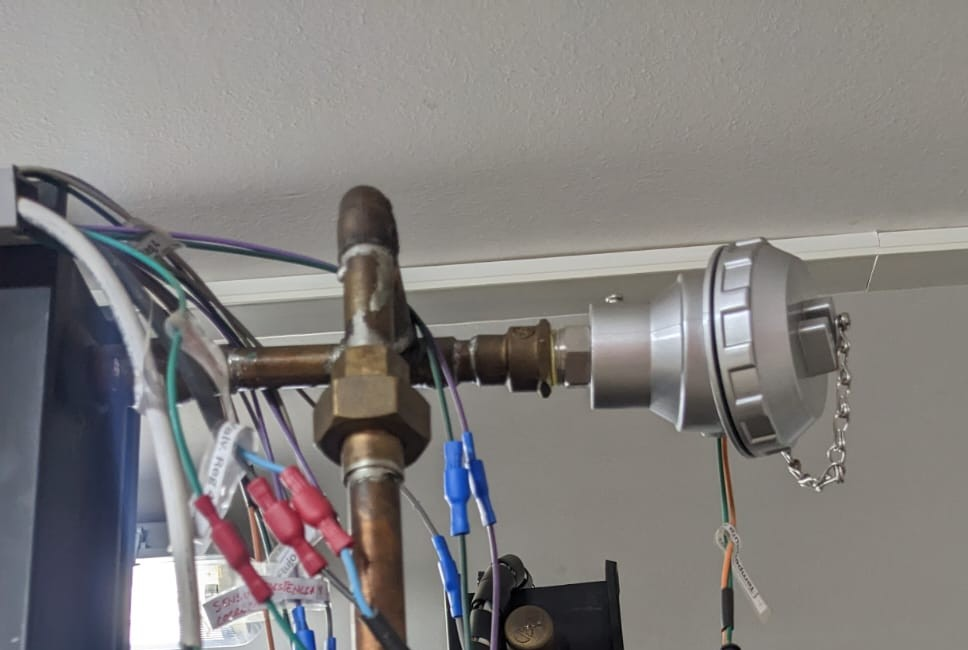
\includegraphics[height=4cm]{termocupla.jpeg}
        \caption{Termocupla.}
    \end{subfigure}
    \begin{subfigure}[b]{0.45\linewidth}
        \centering
        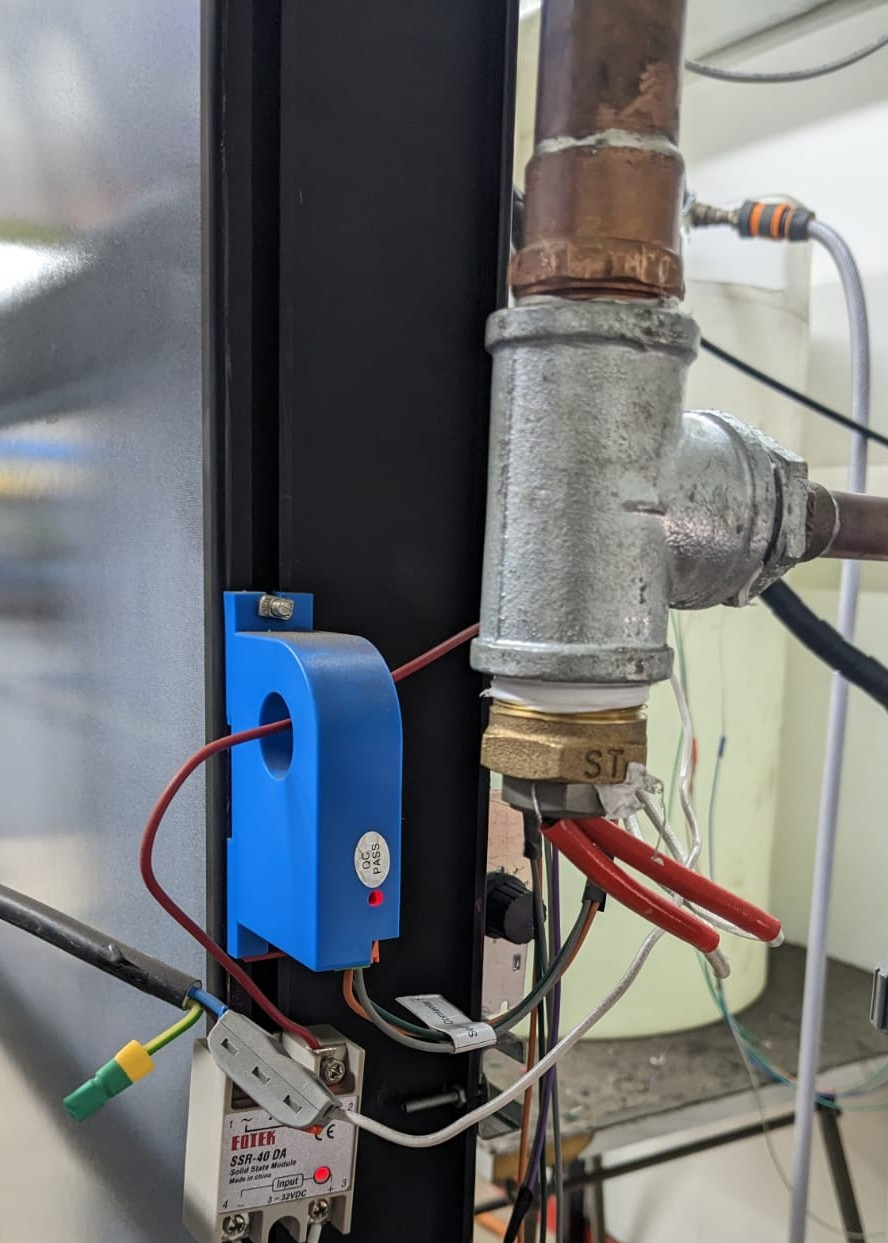
\includegraphics[height=4cm]{resistenciaelectrica.jpeg}
        \caption{Resistencia eléctrica.}
    \end{subfigure}
    \caption{Componentes del sistema.}
    \label{fig:componentes}
\end{figure}

La incorporación de resistencias eléctricas en el banco de ensayos permite disponer de una fuente de calor controlada, repetible y programable. A diferencia de la radiación solar real, que depende de condiciones ambientales variables, las resistencias permiten mantener condiciones experimentales constantes durante los ensayos. Además, permiten reproducir el efecto de una fuente de energía sobre el fluido de trabajo y conservar las características dinámicas relevantes del sistema, tales como el tiempo de retraso, la inercia térmica y la capacidad de almacenamiento de energía de los componentes. Para los objetivos de este estudio, no resulta relevante la forma en la que es entregado el calor, lo importante es que la energía térmica ingresada al sistema genera una respuesta observable en la temperatura de salida. Asimismo, las resistencias eléctricas pueden ser activadas y desactivadas mediante el código de control del sistema, lo  que permite generar variaciones controladas en el aporte de energía térmica. De esta manera, es posible simular perturbaciones o distintas condiciones de operación, representando escenarios similares a los que podrían presentarse en un sistema real. Por lo tanto, el uso de resistencias eléctricas no busca reproducir exactamente la distribución espacial de la radiación solar sobre un colector, sino emular de manera controlada el ingreso de energía térmica al sistema. Bajo este enfoque, las resistencias constituyen un elemento adecuado para estudiar la dinámica térmica del banco de ensayos, facilitar la repetibilidad experimental y generar datos informativos para la identificación del modelo.


Para la adquisición y almacenamiento de los datos experimentales, el banco de pruebas cuenta con un sistema de recolección, observado en la Figura \ref{fig:placeholder}, basado principalmente en un controlador PLC marca Siemens modelo Logo!8 y una tarjeta de adquisición Raspberry Pi 4, los que registran de forma sincronizada las mediciones de temperatura y caudal.
\begin{figure}[H]
    \centering
    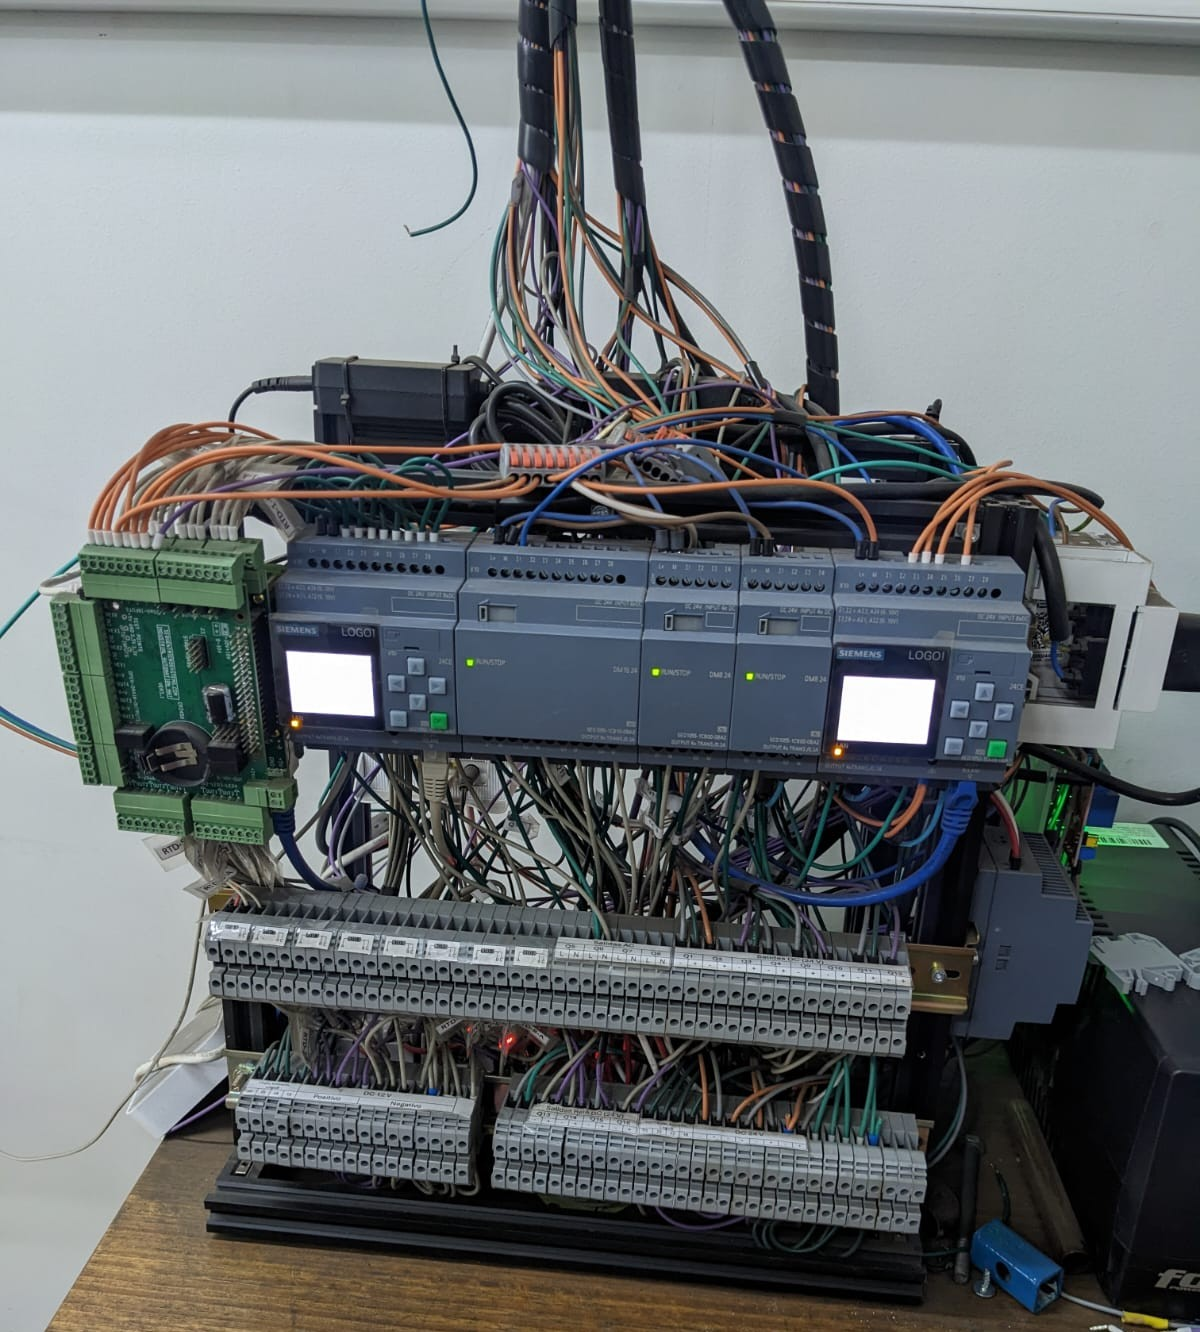
\includegraphics[width=0.5\linewidth]{sistemaelectronico.jpeg}
    \caption{Sistema de adquisición de datos.}
    \label{fig:placeholder}
\end{figure}

\subsubsection{Recorrido del fluido de trabajo}

El agua ingresa desde un estanque al sistema impulsada por la bomba, moviéndose sucesivamente a través de los cuatro paneles termosolares y es calentada de forma progresiva en  cada etapa. A lo largo de este recorrido, el caudal es regulado mediante válvulas proporcionales, mientras que la temperatura del fluido se incrementa debido al aporte energético de las resistencias eléctricas. Las mediciones de temperatura y caudal se registran en distintos puntos a lo largo del sistema, permitiendo analizar la dinámica térmica y su dependencia con las condiciones de operación.







\section{Procedimiento reproducible de identificación y validación}
Con el propósito de establecer una secuencia ordenada y reproducible para el desarrollo de los modelos, se definió un procedimiento general que reúne las principales etapas del proceso de identificación. Este procedimiento comprende desde la definición de las variables y el diseño de las señales de excitación hasta la validación y selección de los modelos obtenidos. Su finalidad es proporcionar una guía general del proceso seguido en este trabajo, mientras que los parámetros específicos, criterios de diseño, resultados experimentales y decisiones adoptadas en cada etapa se desarrollan posteriormente en las secciones correspondientes.
La secuencia propuesta se presenta continuación: 
\begin{enumerate}
    \item \textbf{Definición de las variables del sistema}
    
    En primer lugar, se identifican las variables de entrada y salida del proceso, junto con las restricciones operacionales y las principales características dinámicas que condicionan la identificación. Para el sistema estudiado, inicialmente se consideró una configuración SISO, utilizando el caudal como variable de entrada y la temperatura medida a la salida del último colector como variable de salida. Posteriormente, se incorporó la potencia suministrada por las resistencias eléctricas como una segunda entrada, dando lugar a una configuración MISO y manteniendo la misma variable de salida.

    Como información preliminar para el diseño experimental, se utilizaron antecedentes obtenidos en pruebas realizadas previamente sobre el banco de ensayos, los cuales permitieron disponer de una primera aproximación de los tiempos característicos del sistema y del intervalo de frecuencias en el que se concentra su dinámica relevante.
    
    \item \textbf{Diseño de las señales de excitación}

    Las señales de entrada deben seleccionarse y diseñarse de acuerdo con las características dinámicas del sistema, considerando su amplitud, duración y contenido frecuencial. Un criterio fundamental es que la excitación aporte energía suficiente dentro de la banda de frecuencias donde el proceso presenta una respuesta dinámica significativa.

La selección de la señal depende de las características particulares del sistema y de las variables que se desea manipular. Asimismo, la duración de cada ensayo debe permitir observar adecuadamente los periodos asociados a las frecuencias de interés. En este trabajo se consideran señales PRBS y multisinusoidales, cuyo diseño se desarrolla en las secciones posteriores.

También se deben tener en cuenta las limitaciones físicas de los actuadores y el tiempo de muestreo del sistema de adquisición y control, ya que variaciones excesivamente rápidas pueden no reproducirse físicamente, ser atenuadas por la dinámica del proceso o generar condiciones de operación no deseadas. En configuraciones MISO, además, debe verificarse previamente que las señales de entrada no presenten una dependencia excesiva entre sí, puesto que una elevada correlación puede dificultar la diferenciación de sus efectos individuales sobre la salida y reducir la calidad informativa de los datos obtenidos.


    
    \item \textbf{Aplicación experimental y adquisición de datos}
    
    Una vez diseñadas y verificadas las señales de excitación, estas se aplican al banco de ensayos y se registran simultáneamente las variables de entrada y salida. Durante esta etapa deben mantenerse condiciones experimentales controladas y un periodo de muestreo constante, procurando evitar interrupciones, saturaciones o perturbaciones externas que puedan alterar la información contenida en los registros.
    
    \item \textbf{Evaluación de la calidad de los datos}
    
    Los registros experimentales obtenidos deben ser analizados antes de ser utilizados para la identificación. Para ello, se emplean herramientas como la densidad espectral de potencia, la coherencia, la correlación y la función de respuesta en frecuencia, con el propósito de verificar que las señales aplicadas hayan excitado efectivamente las frecuencias de interés y que exista una relación suficientemente informativa entre las entradas y la salida.

Esta evaluación también permite identificar registros redundantes o conjuntos de datos que no aporten nueva información relevante. Si los datos obtenidos no presentan suficiente contenido informativo, el procedimiento debe regresar a la etapa de diseño de las señales de excitación, modificando sus parámetros y repitiendo el ensayo experimental.

    
    \item \textbf{Preprocesamiento y separación de datos}
   
    Los registros seleccionados se acondicionan antes de la identificación, considerando, cuando corresponda, la eliminación de periodos de estabilización, la sincronización de las señales, el tratamiento de condiciones iniciales y la normalización de las variables.

Posteriormente, los datos se separan en conjuntos independientes destinados a la identificación y validación de los modelos. Para evitar evaluar el modelo con los mismos datos utilizados durante el ajuste de sus parámetros, resulta recomendable disponer de registros experimentales independientes, idealmente obtenidos bajo distintas realizaciones de las señales de excitación o diferentes condiciones de operación.


    \item \textbf{Identificación progresiva de los modelos}
    
La identificación se desarrolla de manera progresiva, comenzando con estructuras de menor complejidad. En una primera etapa se analizan modelos lineales en configuración SISO, con el propósito de caracterizar la relación entre una entrada y la salida del sistema. Posteriormente, se incorporan múltiples entradas mediante estructuras lineales MISO. Si estas estructuras no permiten representar adecuadamente la dinámica observada, se procede a evaluar modelos MISO no lineales.

Esta progresión permite determinar en qué medida el aumento de complejidad estructural contribuye efectivamente a mejorar la representación del comportamiento térmico del sistema.



    
    \item \textbf{Selección de estructuras y parámetros}
   
    Para cada modelo se evalúan diferentes órdenes y configuraciones. La selección debe considerar tanto el desempeño obtenido como la complejidad de la estructura, evitando incrementar innecesariamente el número de parámetros.

Esta etapa también se encuentra condicionada por la capacidad computacional disponible, debido a que un aumento en el número de órdenes, retardos o regresores incrementa el espacio de búsqueda y el costo asociado a la estimación. Una mayor complejidad no implica necesariamente un mejor desempeño, por lo que debe buscarse un equilibrio entre capacidad de representación, generalización y costo computacional.
    \item \textbf{Validación mediante simulación libre}
    
    Los modelos seleccionados se evalúan utilizando registros no empleados durante su identificación. En simulación libre, el modelo recibe las variables de entrada junto con las condiciones iniciales necesarias y posteriormente genera de manera recursiva su propia salida sin utilizar mediciones de la variable real.

Este procedimiento permite evaluar la capacidad del modelo para reproducir autónomamente la evolución temporal del sistema. La respuesta simulada debe compararse gráficamente con la salida experimental para observar diferencias en tendencia, amplitud, retardos y comportamiento dinámico.

    \item \textbf{Evaluación del desempeño}

    La calidad de los modelos se analiza utilizando métricas de error y criterios complementarios en los dominios temporal y frecuencial. La evaluación incluye la comparación entre la salida experimental y la respuesta obtenida mediante simulación libre, junto con el análisis de los residuos y de las características frecuenciales de ambas respuestas.

De esta forma, la selección no se basa únicamente en una métrica global de ajuste, sino también en la capacidad del modelo para representar la dinámica relevante del proceso y en la existencia o ausencia de información significativa remanente en los residuos.


    
    \item \textbf{Selección del modelo final}
  
    
    Finalmente, se selecciona el modelo que presente el mejor compromiso entre capacidad de representación, desempeño en simulación libre, comportamiento de los residuos, similitud temporal y frecuencial respecto del sistema experimental y complejidad estructural.
    
    
    
    
\end{enumerate}

El procedimiento descrito se fundamenta en que la identificación basada en datos requiere disponer de registros experimentales que contengan información suficiente sobre la dinámica del sistema estudiado. En este contexto, la adquisición de datos constituye una etapa crítica, ya que las señales de excitación deben provocar variaciones observables y representativas de la respuesta del proceso. Las herramientas de análisis no paramétrico permiten evaluar directamente estos registros sin imponer previamente una estructura funcional al modelo, facilitando el análisis de la función de respuesta en frecuencia, la coherencia entre señales, la distribución espectral de la energía y la presencia de posibles comportamientos no lineales o alteraciones asociadas al ruido y a las mediciones.

La calidad de la identificación depende, por lo tanto, no solo de la estructura matemática seleccionada posteriormente, sino también de la capacidad de las señales de entrada para excitar adecuadamente la dinámica de interés. Cuando se trabaja con múltiples entradas, este requisito incorpora además la necesidad de reducir la dependencia entre los canales de excitación, de modo que sea posible diferenciar el efecto producido por cada variable manipulada sobre la salida. Posteriormente, mediante el análisis de los datos experimentales y herramientas como la FRF, la coherencia y la correlación, es posible determinar si la información adquirida resulta adecuada para continuar con la identificación o si se requiere modificar las condiciones de excitación y repetir el ensayo.

En el banco de emulación termosolar estudiado, las variables manipuladas corresponden al caudal de agua que circula por el sistema y, posteriormente, a la potencia térmica suministrada mediante las resistencias eléctricas. La modificación del caudal altera el tiempo de residencia del fluido y, con ello, el proceso de transferencia de calor y la velocidad de respuesta térmica. Por su parte, la potencia aplicada mediante las resistencias eléctricas modifica directamente el aporte energético al fluido, permitiendo generar variaciones controladas en su evolución térmica. Como variable de salida se considera la temperatura medida a la salida del último colector.

De este modo, la primera etapa del estudio considera una configuración SISO, en la que se analiza la relación dinámica entre el caudal y la temperatura de salida. Posteriormente, el análisis se amplía hacia una configuración MISO, incorporando simultáneamente el caudal y la potencia térmica como variables de entrada. 

Para obtener registros adecuados para la identificación, las señales aplicadas deben diseñarse de manera que exciten principalmente el intervalo de frecuencias donde el sistema presenta una dinámica significativa. En identificación de sistemas no resulta necesario excitar uniformemente todo el dominio frecuencial, sino garantizar un contenido energético suficiente dentro de la banda relevante para el proceso. Este aspecto resulta especialmente importante en sistemas térmicos, caracterizados por tiempos de respuesta relativamente elevados, inercia térmica y una mayor concentración de su dinámica en bajas frecuencias.

A partir de estos criterios, se realiza una etapa preliminar orientada a caracterizar y diseñar cada una de las señales de excitación. Estas pruebas permitieron ajustar los parámetros de las señales y verificar su compatibilidad con las restricciones físicas y operacionales del montaje. En la sección siguiente se presentan estas pruebas exploratorias, las cuales constituyen la primera aplicación práctica del procedimiento descrito y proporcionan los antecedentes necesarios para la obtención de los conjuntos de datos destinados a la identificación y validación de los modelos.




%El modelado basado en datos se centra en el uso de técnicas no paramétricas que permiten analizar directamente los datos experimentales sin asumir una estructura funcional predefinida del sistema. Estas técnicas, sustentadas en métodos estadísticos, facilitan la estimación de funciones de respuesta en frecuencia (FRF), la identificación de no linealidades y la detección de fallas o problemas en las mediciones. El proceso general incluye varias etapas clave. En primer lugar, el diseño del experimento requiere la selección de señales de excitación adecuadas, con el fin de asegurar que los canales de entrada sean independientes y permitan distinguir entre comportamientos lineales y no lineales. Posteriormente, se realiza el preprocesamiento de datos, que contempla la eliminación de tendencias, la segmentación en períodos y la verificación de la independencia entre las señales de entrada mediante el control de correlación. Luego, se lleva a cabo la estimación de la FRF y el análisis estadístico asociado, utilizando funciones de coherencia y otras herramientas  para detectar la presencia de ruido y no linealidades. En función de estos análisis, se evalúa la calidad de las mediciones y se determina si el sistema puede describirse adecuadamente mediante un modelo lineal o si es necesario recurrir a representaciones más complejas. Esta información se emplea para construir modelos no paramétricos o paramétricos, permitiendo tomar decisiones informadas sobre el nivel de complejidad necesario para representar con precisión la dinámica del sistema analizado \cite{csurcsia2020user}.


%Con el fin de acotar el diseño de las señales de excitación, se realizó un análisis previo de datos experimentales obtenidos en ensayos anteriores a este trabajo. A partir de este análisis se determinó que el sistema opera predominantemente en un rango de frecuencias bajas, comprendido entre 0,0005 Hz y 0.01 Hz, lo cual condiciona directamente el diseño de las señales de entrada que se aplicaran para excitar al sistema.

%También, se definió la amplitud física como el caudal del sistema como $u_0=300 L/h$, con variaciones de $\Delta u$ de 50, 100 y 150 $L/h$. Estos valores se definieron según valores históricos del sistema y según pruebas realizadas para este mismo trabajo, pues se observó que la válvula de flujo no responde a un caudal menor o igual a 100 $L/h$.


\section{Pruebas experimentales exploratorias} 

Antes de realizar las pruebas en el sistema, se definieron ciertos parámetros generales que se mantuvieron constantes durante todos los ensayos. Estos parámetros no dependen del tipo de señal de entrada utilizada, sino que están determinados por las características físicas y operacionales del banco de ensayos. En particular, su selección se relaciona con la dinámica lenta propia del sistema térmico, las limitaciones de operación de la válvula proporcional y el rango de frecuencias de interés considerado para la identificación del modelo. De esta manera, los parámetros fijados son:
\begin{itemize}
    \item \textbf{Intervalo de muestreo ($T_s$)}: De acuerdo con registros históricos y limitaciones instrumentales del sistema, en este trabajo el intervalo de muestreo se fijó en $T=2 $ segundos, independiente de la señal de excitación utilizada. Este valor es consistente con las recomendaciones para el diseño de experimentos de identificación de sistemas descritas por Ljung \cite{ljung1999system}, quien indica que el período de muestreo debe ser coherente con la dinámica relevante del sistema y con las limitaciones físicas del actuador. Dada la dinámica lenta del sistema, en el cual las variaciones relevantes ocurren en una escala del orden de minutos y considerando las características dinámicas de la válvula proporcional utilizada, la cual presenta un tiempo de respuesta que impide la aplicación de variaciones menores, el valor $T_s=2$ segundos resulta adecuado para la adquisición de datos experimentales.
    \item \textbf{Frecuencias ($f_{min}$ y $f_{max}$)}: Con el fin de acotar el diseño de las señales de excitación, se realizó un análisis previo de datos experimentales obtenidos en ensayos anteriores a este trabajo. A partir de este análisis se determinó que el sistema opera predominantemente en un rango de frecuencias bajas, comprendido entre 0.0005 Hz y 0.01 Hz, lo cual condiciona directamente el diseño de las señales de entrada que se aplicarán para excitar al sistema.
    \item \textbf{Amplitud}: La amplitud de la señal determina la magnitud de las variaciones aplicadas al sistema y, por lo tanto, influye directamente en la energía de excitación disponible y en la relación señal-ruido de los datos obtenidos. Su selección debe considerar tanto la necesidad de generar variaciones suficientemente observables en la respuesta como las limitaciones físicas del actuador. Para este trabajo se definió un caudal nominal de $300 L/h$ y una amplitud de variación de $\pm 100 L/h$, de modo que la señal opere aproximadamente entre 200 y 400 $ L/h$. Esta elección se estableció a partir de antecedentes históricos del banco de ensayos y de pruebas preliminares realizadas durante el desarrollo del trabajo. En particular, se observó que el sistema presenta dificultades de operación para caudales iguales o inferiores a 100 $L/h$, por lo que se evitó trabajar en dicho rango y se seleccionó una amplitud que permitiera excitar adecuadamente el sistema manteniendo un margen de operación seguro.
    
    \item \textbf{Duración de cada experimento}: Cada experimento está diseñado para durar una hora (3600 segundos); sin embargo, se le dio al sistema un tiempo de 500 segundos para estabilizarse al comienzo, por lo que el tiempo real de cada experimento fue de $4100$ segundos.
    

\end{itemize}



A partir de los parámetros generales establecidos, se llevaron a cabo distintos ensayos de adquisición de datos, cada uno configurado de acuerdo con las características propias de la señal de excitación utilizada.
\subsection{Experimentos con la señal PRBS} 


\subsubsection{Primer experimento: Exploración de la amplitud de la señal}
%\begin{enumerate}
 %   \item 

En un comienzo, el diseño de la señal de excitación PRBS se realizó utilizando el período de reloj $P=4$ \cite{ljung1999system}. Fijando este valor y estableciendo un tiempo de prueba de 30 minutos (el cual no se consideró en la realidad de los experimentos), se obtuvo un orden de registro de desplazamiento de $n=8$ mediante la ecuación $Tiempo_{Total}=PT_s(2^{n}-1)$.
Definido $n$, se varió en cada experimento el período de reloj ($P$) en 15, 25 y 35, junto con el $\Delta u$  de 50, 100 y 150 $L/h$. En la Tabla \ref{tab:expPRBS} se observan las nueve combinaciones de experimentos que se realizaron al variar cada período de reloj con los diferentes $\Delta u$.


\begin{table}[H]
\caption{Configuración de los experimentos iniciales con la señal PRBS.}
\label{tab:expPRBS}
\centering
\begin{tabular}{|l|c|c|c|}
\hline
\textbf{Exp} &  \textbf{$P$} & \textbf{$\Delta u(L/h)$} \\ \hline
\textbf{E1}  & 15         & 50               \\ \hline
\textbf{E2}  & 15         & 100              \\ \hline
\textbf{E3}  & 15         & 150              \\ \hline
\textbf{E4}  & 25         & 50               \\ \hline
\textbf{E5}  & 25         & 100              \\ \hline
\textbf{E6}  & 25         & 150              \\ \hline
\textbf{E7}  & 35         & 50               \\ \hline
\textbf{E8}  & 35         & 100              \\ \hline
\textbf{E9}  & 35         & 150              \\ \hline
\end{tabular}
\end{table}

 
% Durante el análisis preliminar de los ensayos experimentales, se observaron diferencias aparentes en las métricas de coherencia y en la función de respuesta en frecuencia al comparar registros obtenidos con distintos valores de $\Delta u$. Sin embargo, un examen detallado de los datos reveló que dichos registros presentaban variaciones en el intervalo efectivo entre muestras, aún cuando estos experimentos fueron diseñados con un intervalo de muestreo nominal de 2 segundos. Estas desviaciones, aunque pequeñas en promedio, introducen un nivel apreciable de muestreo irregular, el cual afecta directamente la estimación espectral y la coherencia cuando se aplican métodos que asumen muestreo uniforme, dificultando una comparación directa entre ensayos. Con el objetivo de corregir este efecto y garantizar la comparabilidad de los datos, se realizó un remuestreo de todas las señales a una grilla temporal uniforme común, definida a partir del mayor intervalo de muestreo observado, correspondiente a 2.2 segundos. Las señales de entrada y salida fueron interpoladas sobre dicha grilla y posteriormente sometidas a un procesamiento idéntico que incluyó la selección de una ventana temporal común, la eliminación de tendencias y la estimación espectral mediante parámetros uniformes para todos los ensayos. Este procedimiento permitió eliminar el efecto del muestreo irregular y aislar el impacto real de los parámetros experimentales sobre la dinámica del sistema, evidenciando que las diferencias observadas inicialmente no correspondían a cambios dinámicos significativos, sino a limitaciones asociadas al muestreo original.

El análisis espectral de las pruebas realizadas permitió evaluar la influencia de la amplitud de variación del caudal sobre la información obtenida para la caracterización dinámica del sistema. Para ello, se compararon ensayos realizados con un mismo período de reloj y diferentes amplitudes de excitación. A continuación, se presentan los resultados correspondientes a un período de reloj de 25 segundos y variaciones de caudal de 50, 100 y 150 L/h. El mismo procedimiento fue aplicado a los demás períodos evaluados, observándose tendencias comparables. De esta manera, el análisis permite determinar si el incremento de la amplitud de la señal produce cambios relevantes en la relación entrada-salida o únicamente un aumento del nivel energético de la excitación.



La coherencia entre el caudal y la temperatura, Figura \ref{fig:coherenciaP25Delta10015050}, muestra valores elevados para las tres amplitudes en la región de bajas frecuencias. Desde 0 Hz hasta aproximadamente 0.005 Hz, la coherencia se mantiene mayoritariamente por encima de 0.7 y alcanza valores cercanos a uno en distintas frecuencias, aunque se observan disminuciones puntuales. Este comportamiento indica que, dentro de esta región, existe una relación lineal consistente entre las variaciones del caudal y la respuesta térmica del sistema. Sin embargo, a partir de aproximadamente 0.0055–0.006 Hz la coherencia disminuye de manera importante y presenta mayores fluctuaciones, especialmente para las amplitudes de 100 y 150 L/h. La comparación entre las tres curvas muestra, además, que aumentar la amplitud del caudal no genera una mejora sistemática de la coherencia. La señal con una variación de 150 L/h no presenta valores consistentemente superiores a las configuraciones de 50 y 100 L/h y, en determinadas frecuencias, incluso exhibe una coherencia menor. Por lo tanto, dentro del rango de amplitudes evaluado, un incremento de la excitación no implica necesariamente una relación entrada-salida más consistente ni una mejora directa de la información dinámica obtenida.

 

 
\begin{figure}[H]
    \centering
    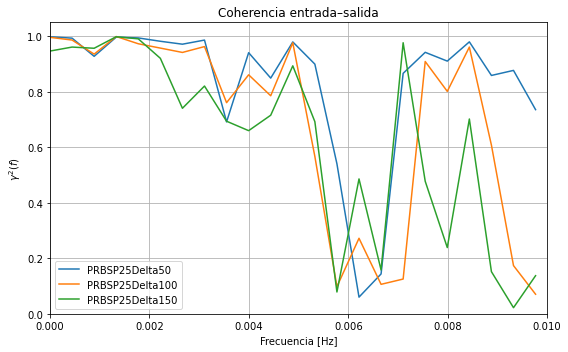
\includegraphics[width=0.5\linewidth]{Figure 2026-08-18 204050 (2).png}
    \caption{Coherencia espectral en los tres experimentos.}
    \label{fig:coherenciaP25Delta10015050}
\end{figure}


En la densidad de potencia de la entrada (Figura \ref{fig:densidadentradap2550100150}), el incremento de la variación del caudal produce, en términos generales, un aumento del contenido energético disponible para excitar el sistema. La señal con una variación de 50 L/h presenta los menores niveles espectrales en gran parte de la banda, mientras que las señales de 100 y 150 L/h proporcionan mayores niveles de excitación. La señal de 150 L/h alcanza los valores más elevados en varias regiones de frecuencia, aunque la distribución espectral no mantiene un orden estrictamente creciente en todos los puntos analizados. La densidad espectral de la salida, Figura \ref{fig:densidadsalidap2550100150}, reproduce una tendencia semejante. El ensayo con una variación de 150 L/h presenta, en términos generales, una mayor respuesta energética de la temperatura, seguido por la configuración de 100 L/h, mientras que el ensayo con 50 L/h presenta los menores niveles. En todos los casos se observa una disminución importante de la densidad espectral con el aumento de la frecuencia, lo que refleja el carácter lento de la dinámica térmica y la atenuación de las componentes de mayor frecuencia.


\begin{figure}[H]
    \centering
    \begin{subfigure}[b]{0.48\textwidth}
        \centering
        \includegraphics[width=\linewidth]{"Figure 2026-08-18 204050 (3)".png}
        \caption{Densidad de entrada.}
        \label{fig:densidadentradap2550100150}
    \end{subfigure}
    \hfill
    \begin{subfigure}[b]{0.48\textwidth}
        \centering
        \includegraphics[width=\linewidth]{"Figure 2026-08-18 204050 (4)".png}
        \caption{Densidad de salida.}
        \label{fig:densidadsalidap2550100150}
    \end{subfigure}
    \caption{Comparación de densidades de entrada y salida.}
    \label{fig:densidades_entrada_salida}
\end{figure}

La función de respuesta en frecuencia presenta un comportamiento similar para los tres niveles de amplitud en la región donde la coherencia alcanza sus mayores valores. En la magnitud (Figura \ref{fig:frfMPRBSDELTAU}) se observa una disminución progresiva al aumentar la frecuencia, con una superposición estrecha de las curvas aproximadamente hasta 0.005 Hz. Esto indica que, en esta región, las tres amplitudes permiten observar una dinámica frecuencial comparable. A partir de aproximadamente 0.006 Hz se produce una mayor separación entre las curvas y aparecen fluctuaciones más pronunciadas. Dado que estas diferencias coinciden con la región en que disminuye la coherencia, la relación lineal entre la entrada y la salida es menos consistente. Por esta razón, las oscilaciones observadas en la magnitud de la FRF a frecuencias mayores no deben interpretarse necesariamente como cambios de la dinámica del sistema provocados por la amplitud de excitación, sino también como una consecuencia de la menor relación señal-ruido y de una mayor incertidumbre en la estimación frecuencial.

La fase, Figura \ref{fig:frfFDELTAU}, presenta un comportamiento equivalente en las bajas frecuencias, donde las tres configuraciones evolucionan de manera similar. Hasta aproximadamente 0.005 Hz, las curvas se mantienen próximas entre sí, mientras que en frecuencias superiores aparecen diferencias más importantes, particularmente para la señal con una variación de 50 L/h. Al igual que en la magnitud, esta separación se presenta principalmente en la región donde la coherencia disminuye, por lo que no necesariamente representa un cambio atribuible exclusivamente a la amplitud de excitación.



\begin{figure}[H]
    \centering
    \begin{subfigure}[b]{0.48\textwidth}
        \centering
        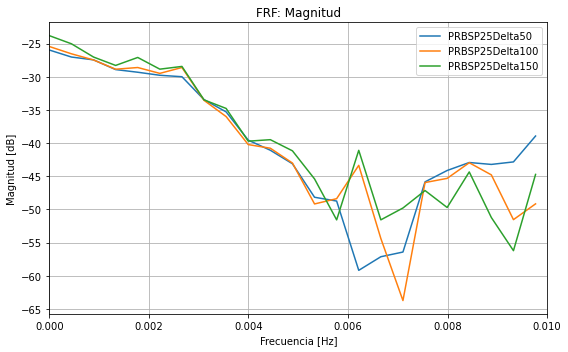
\includegraphics[width=\linewidth]{Figure 2026-08-21 143810 (0).png}
        \caption{Magnitud.}
        \label{fig:frfMPRBSDELTAU}
    \end{subfigure}
    \hfill
    \begin{subfigure}[b]{0.48\textwidth}
        \centering
        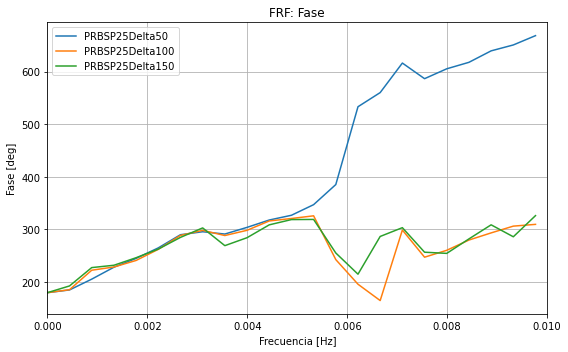
\includegraphics[width=\linewidth]{Figure 2026-08-21 143810 (1).png}
        \caption{Fase.}
        \label{fig:frfFDELTAU}
    \end{subfigure}
    \caption{FRF en los tres ensayos con $P=25$: Magnitud y Fase.}
    \label{fig:frf_ensayos_P25}
\end{figure}

En conjunto, los resultados muestran que el principal efecto de aumentar la amplitud de variación del caudal es incrementar la energía introducida al sistema y, consecuentemente, el nivel energético de la respuesta térmica. Sin embargo, este incremento no se traduce en una mejora sistemática de la coherencia ni en diferencias relevantes en la función de respuesta en frecuencia dentro de la región donde la relación entrada-salida es más consistente. Por lo tanto, no se observa una ventaja suficiente que justifique utilizar la máxima amplitud de excitación en los análisis posteriores.

En función de estos resultados, se seleccionó una variación de caudal de 100 L/h como amplitud de referencia. Esta configuración representa una condición intermedia que proporciona un nivel de excitación claramente superior al obtenido con 50 L/h, sin requerir la amplitud adicional de 150 L/h, la cual no entrega una mejora consistente en términos de coherencia o caracterización de la respuesta frecuencial. La selección de este valor permite, además, mantener la señal dentro de un rango de operación adecuado para el sistema y reducir el número de combinaciones necesarias en las etapas posteriores del estudio.

A partir de esta selección, la amplitud de variación del caudal se mantuvo constante en 100 L/h y los análisis posteriores se concentraron en el estudio de los parámetros que determinan la distribución temporal y frecuencial de las señales de excitación.


%En los gráficos de coherencia, Figura \ref{fig:coherenciaP25Delta10015050}, se aprecia que esta no corresponde a una curva suave, sino que presenta un comportamiento altamente disperso, con valores altos cercanos a 1 e intercalados con valores bajos cercanos a 0 a lo largo del rango de frecuencia analizado. De acuerdo con Ljung \cite{ljung1999system},este patrón es característico de sistemas reales, donde la relación lineal entrada-salida es intermitentemente dominante en  frecuencia. Un aspecto relevante es que las curvas de coherencia asociadas a los distintos valores de $\Delta u$ se superponen estadísticamente, lo que indica que la variación de la amplitud de la excitación no altera la estructura de dependencia lineal entre la entrada y la salida.


%Cabe destacar que no se muestra el análisis independiente de la densidad espectral como criterio adicional de selección. En efecto, la estimación de coherencia y de la FRF se basa directamente en las densidades espectrales de la entrada, de la salida y de la densidad espectral cruzada, calculadas de manera consistente mediante el mismo estimador espectral.



%\item 
\subsubsection{Segundo experimento: Exploración del periodo de reloj y definición final de la señal PRBS}
Para diseñar las señales PRBS se utilizaron afirmaciones de Ljung \cite{ljung1999system} que no se tuvieron en cuenta en experimentos anteriores:
\begin{enumerate}[label=\roman*)]
    \item Las propiedades de ruido blanco de la PRBS son válidas cuando el registro contiene períodos completos, por lo tanto, es esencial que se cumpla $MPT_s\leq3600s$, con lo cual se asegura que al menos se complete un período.
    \item Al tener fijo el intervalo de muestreo en $T_s=2 $ segundos, se define que el período de reloj cumpla con $P\geq15$, así los cambios de valor serán al menos cada $T_sP=30$ segundos. Al utilizar un $P$ más pequeño, los cambios en el caudal se hacen más rápidos, lo que podría causar errores o fallas físicas al sistema.
    \item Al aumentar período de reloj $P$, la señal deja de excitar frecuencias altas, por lo tanto, según Ljung \cite{ljung1999system}, no se pueden excitar frecuencias mayores que el orden de $1/PT_s$, obteniendo el criterio de $f_{max}\approx1/(2PT_s)$.
    \item Dado que la PRBS es periódica, la frecuencia menor excitada corresponde al inverso del periodo completo de la señal. En consecuencia $f_{min}\leq1/(MPT_s)$
\end{enumerate}


Con estos criterios, se diseña una señal PRBS con $n=6$, $M=63$ y con la restricción de $15\leq P\leq25$, por lo que se tomaron muestras con $P=15$, $P=20$ y $P=25$.

La Figura \ref{fig:seis_imagenes} presenta las señales de entrada y salida obtenidas a partir de las tres configuraciones de señales PRBS aplicadas al sistema. En cada caso, el caudal actúa como variable manipulada, mientras que la temperatura constituye la variable de respuesta.



\begin{figure}[H]
    \centering
    % --- FILA 1 ---
    \begin{subfigure}[b]{0.48\linewidth} % Alineación [b]
        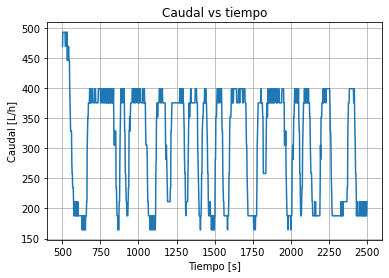
\includegraphics[width=\linewidth]{prbs p=15 entrada.png} % Usa \linewidth aquí
        \caption{Entrada del sistema con PRBS, P=15.}
        \label{fig:ENTRADAP15}
    \end{subfigure}
    \hfill
    \begin{subfigure}[b]{0.48\linewidth} % CAMBIO: [b] en lugar de [H]
        \centering
        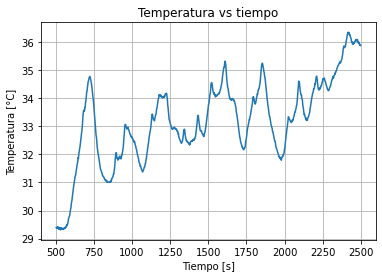
\includegraphics[width=\linewidth]{prbs p=15 salida.png} % Usa \linewidth aquí
        \caption{Salida del sistema con PRBS, P=15.}
        \label{fig:SalidaP15}
    \end{subfigure}
    \\[2ex] % <--- SALTO DE LÍNEA con espacio extra

    % --- FILA 2 ---
    \begin{subfigure}[b]{0.45\linewidth}
        \centering
        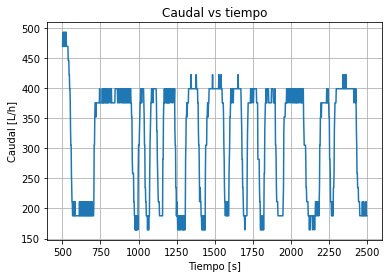
\includegraphics[width=\linewidth]{prbs p=20 entrada.png}
        \caption{Entrada del sistema con PRBS, P=20.}
        \label{fig:entrada20}
    \end{subfigure}
    \hfill
    \begin{subfigure}[b]{0.45\linewidth}
        \centering
        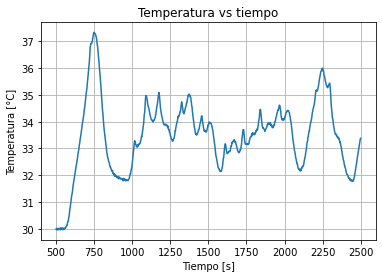
\includegraphics[width=\linewidth]{prbs p=20 salida.png}
        \caption{Salida del sistema con PRBS, P=20.}
        \label{fig:SalidaP20}
    \end{subfigure}
    \\[2ex]

    % --- FILA 3 ---
    \begin{subfigure}[b]{0.45\linewidth}
        \centering
        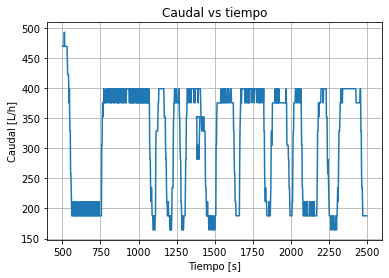
\includegraphics[width=\linewidth]{prbs p=25 entrada.png}
        \caption{Entrada del sistema con PRBS, P=25.}
        \label{fig:entrada25}
    \end{subfigure}
    \hfill
    \begin{subfigure}[b]{0.45\linewidth}
        \centering
        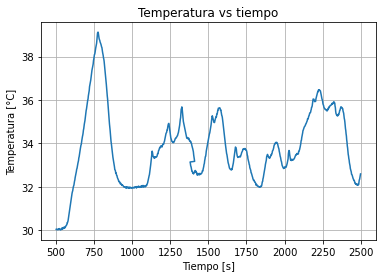
\includegraphics[width=\linewidth]{prbs p=25 salida.png}
        \caption{Salida del sistema con PRBS, P=25.}
        \label{fig:SalidaP25}
    \end{subfigure}

    \caption{Entrada y salida de los tres experimentos con la señal PRBS con $n=6$.}
    \label{fig:seis_imagenes}
\end{figure}

Una vez establecida la amplitud de variación del caudal, el análisis de las señales PRBS se concentró en estudiar la influencia del período de reloj sobre la información obtenida del sistema. Para ello, se realizaron tres ensayos manteniendo constante la amplitud de excitación y utilizando períodos de reloj de 15, 20 y 25 segundos. Los registros obtenidos fueron comparados mediante la coherencia entrada-salida, las densidades espectrales de potencia de entrada y salida y la función de respuesta en frecuencia, considerando la banda comprendida entre 0 y 0.01 Hz.

La coherencia entre el caudal y la temperatura (Figura \ref{fig:coherenciaprbs151304}) presenta un comportamiento con algunas variaciones a lo largo de la banda analizada. En las frecuencias inferiores se observan valores moderados, aproximadamente entre 0.5 y 0.7, mientras que alrededor de 0.004 Hz las tres señales alcanzan nuevamente valores cercanos o superiores a 0.5. Posteriormente, la coherencia disminuye de manera importante hacia aproximadamente 0.007–0.008 Hz, para luego presentar una recuperación parcial hacia el extremo superior de la banda.
Este comportamiento indica que la relación lineal entre las variaciones del caudal y la respuesta de temperatura depende de la frecuencia y no presenta la misma intensidad en todo el intervalo considerado. Sin embargo, las tres señales exhiben tendencias comparables y ninguna de las configuraciones presenta una coherencia sistemáticamente superior en toda la banda. Por lo tanto, la modificación del período de reloj entre 15 y 25 segundos no produce, por sí sola, una mejora generalizada de la relación entrada-salida.



\begin{figure}[H]
    \centering
    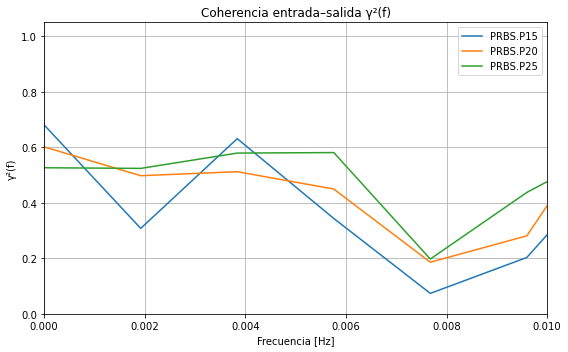
\includegraphics[width=0.5\linewidth]{Figure 2026-08-18 215026 (0).png}
    \caption{Comparación de la coherencia espectral entre los ensayos con PRBS.}
    \label{fig:coherenciaprbs151304}
\end{figure}

La densidad espectral de potencia de la entrada mostrada en la Figura \ref{fig:densidadentradaPRBS} permite observar con mayor claridad las diferencias producidas por el período de reloj. Las tres configuraciones presentan contenido energético dentro de la banda analizada, aunque su distribución no es idéntica. En particular, la señal con P = 25 presenta los mayores niveles de densidad espectral en la región de frecuencias más bajas, seguida por las configuraciones P = 20 y P = 15. A medida que aumenta la frecuencia, las diferencias disminuyen y las densidades espectrales convergen progresivamente hacia valores similares próximos a 0.01 Hz. Este resultado es consistente con el efecto esperado al aumentar el período de reloj de una señal PRBS. Un mayor período implica que cada nivel de la señal se mantiene durante un tiempo más prolongado, desplazando una mayor proporción de su contenido energético hacia frecuencias bajas. Esta característica resulta particularmente relevante para el sistema térmico estudiado, debido a que su dinámica dominante se desarrolla principalmente en esta región frecuencial. En consecuencia, las tres señales excitan la banda considerada, pero P = 25 proporciona una mayor concentración de energía en la zona asociada a las dinámicas más lentas.

La densidad espectral de potencia de la salida, Figura \ref{fig:densidadsalidaPRBS}, presenta una tendencia semejante para los tres ensayos. La mayor energía de la respuesta térmica se concentra en las frecuencias inferiores y disminuye de manera pronunciada al aumentar la frecuencia. Esta disminución evidencia el carácter lento de la dinámica térmica y la atenuación de las componentes de mayor frecuencia. Además, la configuración con P = 25 presenta los mayores niveles de densidad espectral de salida en las frecuencias bajas, seguida por P = 20 y P = 15, manteniéndose una forma general comparable entre los tres experimentos.





\begin{figure}[H]
    \centering
    \begin{subfigure}[b]{0.48\textwidth}
        \centering
        \includegraphics[width=\linewidth]{"Figure 2026-08-18 215026 (2)".png}
        \caption{Densidad de entrada.}
        \label{fig:densidadentradaPRBS}
    \end{subfigure}
    \hfill
    \begin{subfigure}[b]{0.48\textwidth}
        \centering
        \includegraphics[width=\linewidth]{"Figure 2026-08-18 215026 (3)".png}
        \caption{Densidad de salida.}
        \label{fig:densidadsalidaPRBS}
    \end{subfigure}
    \caption{Comparación de densidad espectral de entrada y salida entre los ensayos PRBS.}
    \label{fig:densidades_PRBS}
\end{figure}


 En términos de magnitud (Figura \ref{fig:FRFmagnitud152025}), la FRF de las tres configuraciones presentan una tendencia prácticamente equivalente dentro de la banda estudiada. La magnitud disminuye progresivamente con el aumento de la frecuencia, evidenciando una mayor respuesta del sistema frente a variaciones lentas del caudal y una mayor atenuación frente a variaciones más rápidas. Si bien existen pequeñas diferencias entre los ensayos, no se observan cambios importantes en la forma general de las curvas ni desplazamientos sistemáticos que permitan asociar un comportamiento dinámico diferente a alguno de los períodos evaluados. La fase de la función de respuesta en frecuencia, (Figura \ref{fig:FRFfasePRBS152025}), presenta igualmente una evolución similar para las tres configuraciones. Las curvas permanecen próximas entre sí en gran parte de la banda, mostrando que el cambio del período de reloj no genera modificaciones sustanciales en el desfase observado entre la entrada de caudal y la respuesta térmica.




\begin{figure}[H]
    \centering
    \begin{subfigure}[b]{0.48\textwidth}
        \centering
        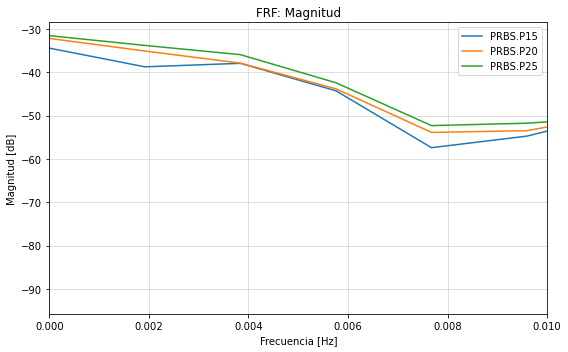
\includegraphics[width=\linewidth]{frfMAGINTUD.png}
        \caption{Magnitud.}
        \label{fig:FRFmagnitud152025}
    \end{subfigure}
    \hfill
    \begin{subfigure}[b]{0.48\textwidth}
        \centering
        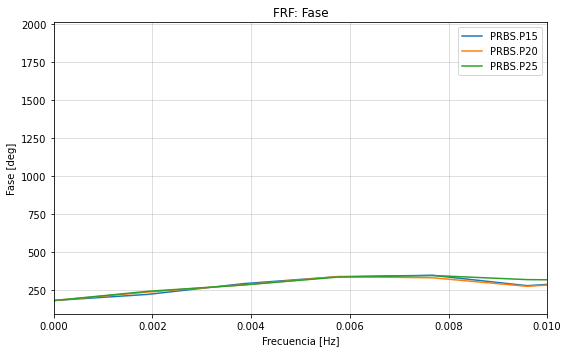
\includegraphics[width=\linewidth]{FRFfasePRBS.png}
        \caption{Fase.}
        \label{fig:FRFfasePRBS152025}
    \end{subfigure}
    \caption{Respuesta en frecuencia (FRF): Magnitud y Fase.}
    \label{fig:FRF_PRBS_152025}
\end{figure}



A partir de estos resultados, se seleccionó la configuración con P = 25 segundos para las etapas posteriores de identificación. Esta elección no se fundamenta en que dicha señal presente una coherencia superior en toda la banda ni en que genere una dinámica diferente, sino en que proporciona una mayor excitación en la región de bajas frecuencias, donde se concentra principalmente la respuesta del sistema térmico. Al mismo tiempo, su función de respuesta en frecuencia mantiene una tendencia consistente con las configuraciones P = 15 y P = 20, lo que indica que el aumento del período de reloj no introduce modificaciones relevantes en la dinámica observada.

Adicionalmente, un período de reloj de 25 segundos implica que la señal PRBS mantiene cada nivel durante un intervalo mayor de tiempo, evitando cambios excesivamente rápidos o demasiado breves en el caudal. Esto resulta conveniente para un sistema térmico de dinámica lenta, ya que favorece transiciones más suaves en la excitación y ayuda a atenuar cambios bruscos que el sistema difícilmente podría reproducir de manera representativa. En este sentido, la configuración con P = 25 no solo concentra mayor energía en bajas frecuencias, sino que también genera una excitación más acorde con la inercia térmica del proceso estudiado.

De este modo, P = 25 segundos representa una alternativa adecuada para caracterizar la dinámica lenta del sistema, ya que combina una mayor concentración de energía en la región frecuencial de mayor interés con una respuesta térmica y una función de respuesta en frecuencia consistentes con las obtenidas en los demás ensayos. Además, al reducir la presencia de cambios repentinos en la señal de entrada, permite excitar el sistema de una forma más compatible con su comportamiento físico.





\subsection{Experimentos con la señal multisinusoidal}
\subsubsection {Exploración del número de componentes}
Para la generación de las señales multisinusoidales se consideraron los resultados obtenidos previamente en los ensayos realizados con señales PRBS. A partir de dicho análisis, se observó que la amplitud de variación del caudal no afectaba de manera apreciable la dinámica del sistema dentro de la banda de frecuencias de interés. En consecuencia, se definió un valor fijo de amplitud de excitación de $\Delta u = 100 L/h$ para todos los ensayos con señales multisinusoidales. De esta forma, el diseño de las señales se concentró únicamente en la variación del número de componentes sinusoidales utilizadas, manteniendo constante la amplitud del caudal. Esta decisión permitió reducir el número de combinaciones evaluadas y focalizar el análisis en el efecto de la distribución frecuencial de la señal sobre la capacidad de excitación del sistema térmico.
\begin{enumerate}[label=\roman*)]
\item Es importante utilizar períodos enteros \cite{ljung1999system}, es por ello que, dada la duración del experimento (1 hora), se seleccionó un $M$ igual a 900 muestras, lo que permite observar exactamente dos períodos completos en la ventana experimental. Esta elección mantiene una resolución espectral muy cercana a la frecuencia mínima de interés y garantiza la periodicidad de la señal en la ventana de análisis, evitando efectos de fuga espectral.
\item El número de sinusoides $d$ se seleccionó teniendo en cuenta la cobertura espectral suficiente y la factibilidad experimental \cite{ljung1999system}. Entonces, según la selección de $M$ y $T_s$ ya definido, se obtiene que el periodo fundamental de la señal  es de 1800 segundos ($900\cdot2s$), teniendo una resolución espectral mínima (rejilla DFT) de 0.00056 Hz ($1/1800s$). Esto quiere decir que la señal puede excitar frecuencias separadas por 0.00056 Hz. Según la banda útil de frecuencias definida, existen hasta 23 líneas espectrales disponibles. Además, $d$ debe ser lo suficientemente grande para cubrir la banda con resolución útil. Es por ello que se experimentará con $d$ igual a 23, 16 y 10. 









\end{enumerate}





La Figura \ref{fig:seis_imagenesmultiseno} muestra las señales de entrada asociadas a las tres configuraciones de la señal multisinusoidal, acompañadas por la correspondiente respuesta de temperatura del sistema.
   

\begin{figure}[H]
    \centering
    % --- FILA 1 ---
    \begin{subfigure}[b]{0.48\textwidth}
        \centering
        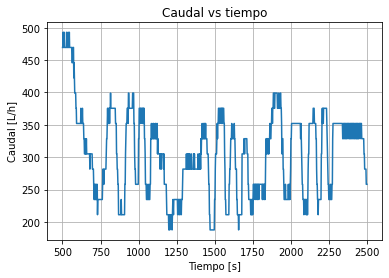
\includegraphics[width=\linewidth, height=0.22\textheight, keepaspectratio]{caudalmultisenod10.png}
        \caption{Entrada del sistema ($d=10$).}
        \label{fig:ENTRADAd10}
    \end{subfigure}
    \hfill
    \begin{subfigure}[b]{0.48\textwidth}
        \centering
        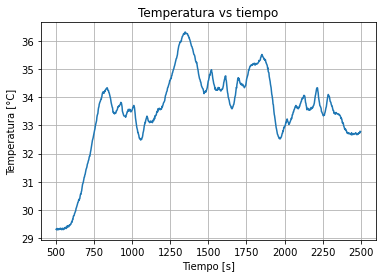
\includegraphics[width=\linewidth, height=0.22\textheight, keepaspectratio]{temperaturamiltisenod10.png}
        \caption{Salida del sistema ($d=10$).}
        \label{fig:Salidad10}
    \end{subfigure}

    \vspace{0.5em}

    % --- FILA 2 ---
    \begin{subfigure}[b]{0.48\textwidth}
        \centering
        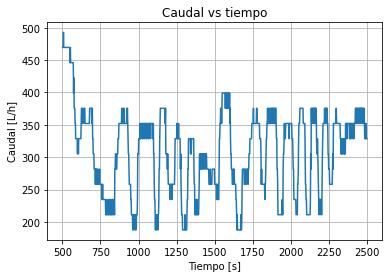
\includegraphics[width=\linewidth, height=0.22\textheight, keepaspectratio]{caudalmultisenod16.png}
        \caption{Entrada del sistema ($d=16$).}
        \label{fig:entradad16}
    \end{subfigure}
    \hfill
    \begin{subfigure}[b]{0.48\textwidth}
        \centering
        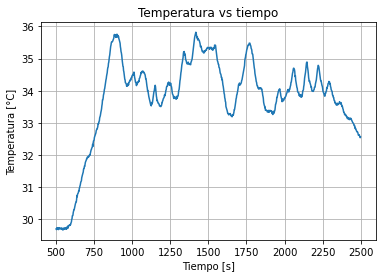
\includegraphics[width=\linewidth, height=0.22\textheight, keepaspectratio]{temperaturamultisenod16.png}
        \caption{Salida del sistema ($d=16$).}
        \label{fig:Salidad16}
    \end{subfigure}

    \vspace{0.5em}

    % --- FILA 3 ---
    \begin{subfigure}[b]{0.48\textwidth}
        \centering
        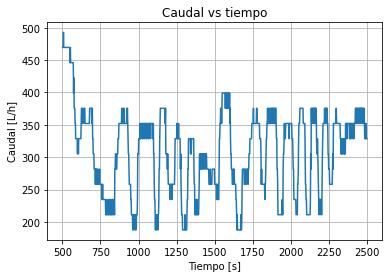
\includegraphics[width=\linewidth, height=0.22\textheight, keepaspectratio]{caudalmultisenod23.png}
        \caption{Entrada del sistema ($d=23$).}
        \label{fig:entrada23}
    \end{subfigure}
    \hfill
    \begin{subfigure}[b]{0.48\textwidth}
        \centering
        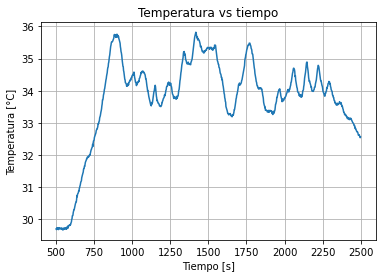
\includegraphics[width=\linewidth, height=0.22\textheight, keepaspectratio]{temperaturamultisenod23.png}
        \caption{Salida del sistema ($d=23$).}
        \label{fig:Salidad23}
    \end{subfigure}

    \caption{Entrada y salida de los tres experimentos con la señal multisinusoidal con $M=900$.}
    \label{fig:seis_imagenesmultiseno}
\end{figure}






           
Los datos resultantes de estos experimentos se analizaron considerando los criterios espectrales relevantes para la identificación de sistemas y se concentró en el intervalo comprendido entre 0 y 0.01 Hz, correspondiente a la zona de bajas frecuencias de interés para caracterizar la dinámica térmica del sistema. 

En primer lugar, la coherencia entre la entrada y la salida muestra un comportamiento dependiente de la frecuencia para las tres configuraciones evaluadas (Figura \ref{fig:coherenciamultiseno}). En las frecuencias más bajas se observan valores cercanos a 0.9, evidenciando una relación importante entre las variaciones del caudal y la respuesta térmica del sistema. A medida que aumenta la frecuencia, la coherencia disminuye y presenta fluctuaciones, alcanzando valores aproximadamente entre 0.3 y 0.7 en distintos sectores de la banda analizada. Las tres configuraciones presentan tendencias similares, aunque con diferencias locales en determinadas frecuencias. En particular, no se observa que un número mayor de componentes sinusoidales produzca de manera sistemática una coherencia superior en toda la banda. %Por lo tanto, los resultados indican que la relación entrada-salida es más consistente en las frecuencias inferiores, mientras que en las frecuencias más altas de la banda analizada aumenta la contribución de efectos no explicados. 

\begin{figure}[H]
    \centering
    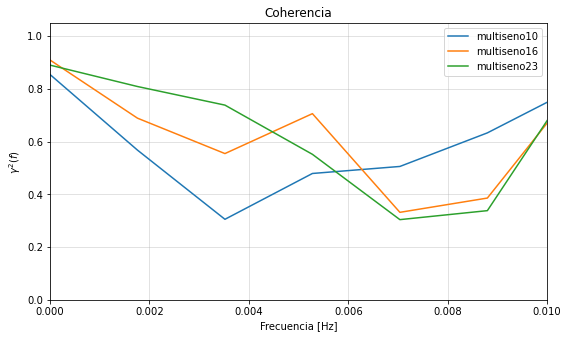
\includegraphics[width=0.5\linewidth]{Figure 2026-08-21 115951 (0).png}
    \caption{Comparación de la coherencia espectral entre los experimentos con la señal multisinusoidal.}
    \label{fig:coherenciamultiseno}
\end{figure}


El análisis de la densidad espectral de potencia de la señal de entrada  (Figura \ref{fig:denen}) muestra una elevada concentración de energía en las frecuencias más bajas, seguida de una disminución pronunciada al aumentar la frecuencia. A partir de aproximadamente 0.0035 Hz, los niveles de densidad espectral se reducen considerablemente y presentan variaciones menores hasta alcanzar 0.01 Hz. Las tres configuraciones muestran un comportamiento semejante, aunque las señales con 16 y 23 componentes exhiben distribuciones similares, con pequeñas diferencias locales asociadas a la distribución de las componentes sinusoidales. En conjunto, los resultados muestran que las tres señales concentran una fracción importante de su contenido energético en la región de bajas frecuencias, concordante con la dinámica lenta característica del sistema térmico.

Por su parte, la densidad espectral de potencia de la salida (Figura \ref{fig:densal}) presenta una disminución aún más marcada con el aumento de la frecuencia. Los mayores valores se concentran en las frecuencias inferiores, mientras que la energía de la respuesta térmica disminuye rápidamente y alcanza valores próximos a cero hacia el extremo superior de la banda analizada. Las curvas correspondientes a las tres configuraciones prácticamente se superponen en todo el intervalo frecuencial, evidenciando que el sistema responde de manera muy similar frente a las distintas señales multisinusoidales. Este comportamiento también refleja el carácter predominantemente lento de la dinámica térmica, cuya respuesta se concentra principalmente en las componentes de menor frecuencia.







\begin{figure}[H]
    \centering
    \begin{subfigure}[b]{0.48\textwidth}
        \centering
        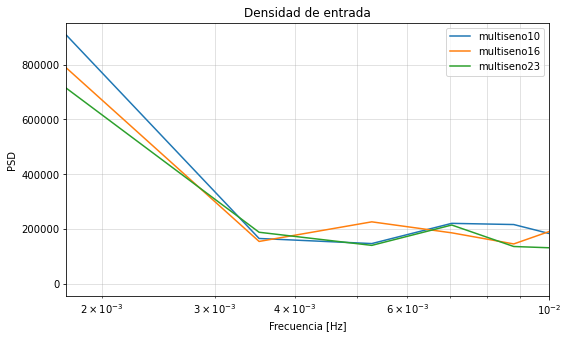
\includegraphics[width=\linewidth]{Figure 2026-08-21 115951 (1).png}
        \caption{PSD en la entrada.}
        \label{fig:denen}
    \end{subfigure}
    \hfill
    \begin{subfigure}[b]{0.48\textwidth}
        \centering
        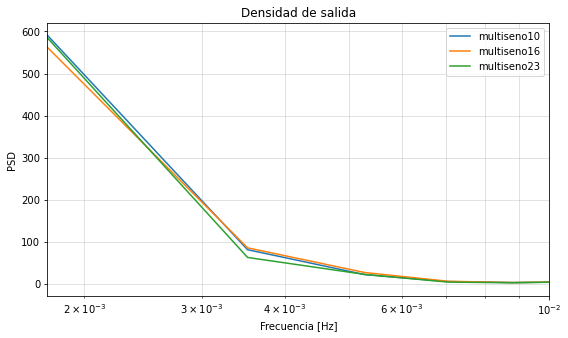
\includegraphics[width=\linewidth]{Figure 2026-08-21 115951 (2).png}
        \caption{PSD en la salida.}
        \label{fig:densal}
    \end{subfigure}
    \caption{Comparación de la densidad espectral en la entrada y en la salida.}
    \label{fig:densidad_espectral}
\end{figure}

La comparación de las funciones de respuesta en frecuencia permite complementar este análisis. En términos de magnitud, Figura \ref{fig:frfmultisenoM}, las tres configuraciones presentan curvas prácticamente coincidentes. La magnitud disminuye progresivamente con la frecuencia, lo que evidencia una atenuación creciente de las componentes de mayor frecuencia, consistente con el comportamiento dinámico esperado para un sistema térmico. Las pequeñas diferencias entre las configuraciones no modifican la tendencia general de la respuesta. De manera similar, la fase de la función de respuesta en frecuencia, Figura \ref{fig:frfmultisenoF},  muestra una evolución comparable para los tres ensayos. Las curvas presentan un incremento de fase en las frecuencias inferiores, seguido de variaciones relativamente pequeñas hacia la zona superior de la banda. La proximidad entre las tres respuestas de fase, al igual que lo observado en la magnitud, indica que la modificación del número de componentes sinusoidales no genera cambios apreciables en la dinámica frecuencial observada del sistema bajo las condiciones de operación consideradas.




\begin{figure}[H]
    \centering
    \begin{subfigure}[b]{0.48\textwidth}
        \centering
        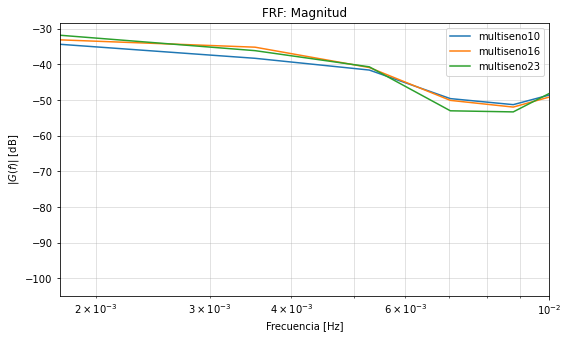
\includegraphics[width=\linewidth]{Figure 2026-08-21 115951 (3).png}
        \caption{Magnitud.}
        \label{fig:frfmultisenoM}
    \end{subfigure}
    \hfill
    \begin{subfigure}[b]{0.48\textwidth}
        \centering
        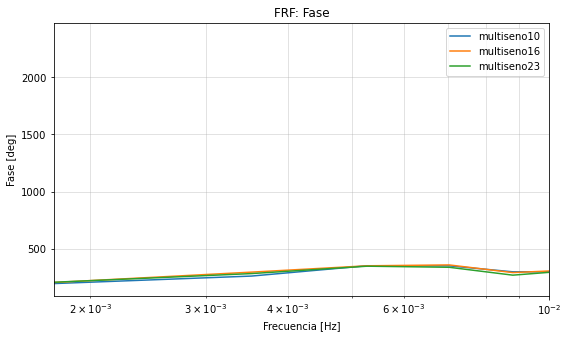
\includegraphics[width=\linewidth]{Figure 2026-08-21 115951 (4).png}
        \caption{Fase.}
        \label{fig:frfmultisenoF}
    \end{subfigure}
    \caption{Respuesta en frecuencia: Magnitud y fase.}
    \label{fig:frfmultiseno}
\end{figure}


En conjunto, los resultados muestran que las tres señales multisinusoidales permiten excitar y caracterizar la dinámica del sistema dentro de la banda analizada. Las mayores diferencias se presentan en la distribución de energía de las señales de entrada y en algunos valores puntuales de coherencia, mientras que la densidad espectral de la salida y las funciones de respuesta en frecuencia presentan una elevada similitud. Esto indica que la variación del número de componentes sinusoidales entre 10, 16 y 23 no modifica de manera significativa la dinámica observada del sistema, sino principalmente la forma en que la excitación se distribuye dentro de la banda de frecuencias considerada. Esto es coherente con el propósito de evaluar diferentes distribuciones frecuenciales manteniendo constante la amplitud de excitación.

A partir de esta comparación, se seleccionó la señal multisinusoidal con 23 componentes como conjunto de validación. Esta elección no se fundamenta en una respuesta dinámica superior ni en una coherencia sistemáticamente mayor, sino en que esta configuración incorpora el mayor número de componentes dentro de la banda considerada y, por tanto, proporciona una cobertura frecuencial más amplia. Esta característica permite someter al modelo a una excitación más rica y distribuida, manteniendo al mismo tiempo una respuesta frecuencial consistente con las demás configuraciones evaluadas.

De esta forma, los datos obtenidos con la señal de 23 componentes se reservaron para comprobar la capacidad del modelo para reproducir la dinámica del sistema frente a una condición de excitación distinta a la utilizada en la identificación. Su utilización como conjunto independiente permite evaluar de manera más exigente la capacidad de generalización del modelo dentro del rango frecuencial relevante para el sistema térmico estudiado.



\subsubsection{Datos obtenidos bajo diferentes condiciones de operación}



Se realizó un ensayo adicional utilizando una señal multisinusoidal aplicada a la entrada de caudal. La señal fue diseñada siguiendo los mismos criterios empleados para la configuración de 23 componentes utilizada anteriormente, manteniendo tanto el número de componentes sinusoidales como la banda de frecuencias de excitación. La principal diferencia corresponde a las condiciones de operación, ya que este nuevo conjunto de datos fue obtenido durante el período invernal. De esta manera, se dispone de un registro independiente adquirido bajo condiciones térmicas distintas a aquellas utilizadas en los ensayos realizados durante el verano.



En el dominio temporal, el caudal presenta una variación aproximadamente comprendida entre 260 y 425 L/h, manteniendo el comportamiento oscilatorio característico de la señal multisinusoidal aplicada, como se observa en la Figura \ref{fig:cuadalsisoinvierno}. La temperatura de salida, mostrada en la Figura \ref{fig:temperatursisoinvierno}, presenta una evolución suave y oscilatoria, con valores aproximados entre 23 °C y 25.5 °C. Estas mediciones muestran que, aun cuando se mantiene el criterio de excitación utilizado anteriormente, el ensayo se desarrolla sobre un nivel térmico diferente. Al tratarse de un experimento realizado en invierno, es esperable que las pérdidas térmicas hacia el ambiente tengan una mayor influencia sobre la respuesta medida, modificando la amplitud de la temperatura respecto de las pruebas anteriores.
\begin{figure}[H]
    \centering
    % Primera subfigura (arriba)
    \begin{subfigure}[b]{0.85\linewidth}
        \centering
        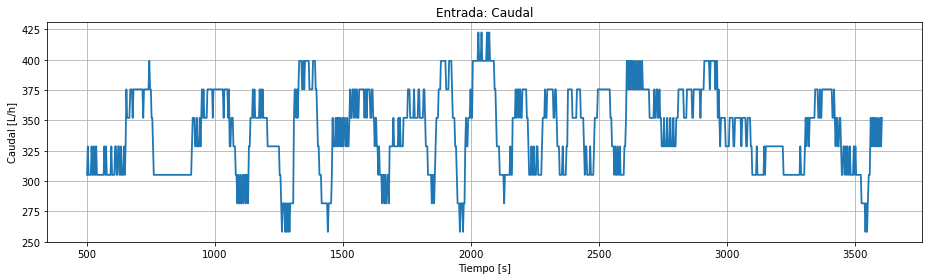
\includegraphics[width=\linewidth]{Figure 2026-07-09 144742.png}
        \caption{Caudal obtenido con señal multisinusoidal.}
        \label{fig:cuadalsisoinvierno}
    \end{subfigure}
    
    \vspace{0.5cm} % Espacio vertical opcional entre figuras
    
    % Segunda subfigura (abajo)
    \begin{subfigure}[b]{0.85\linewidth}
        \centering
        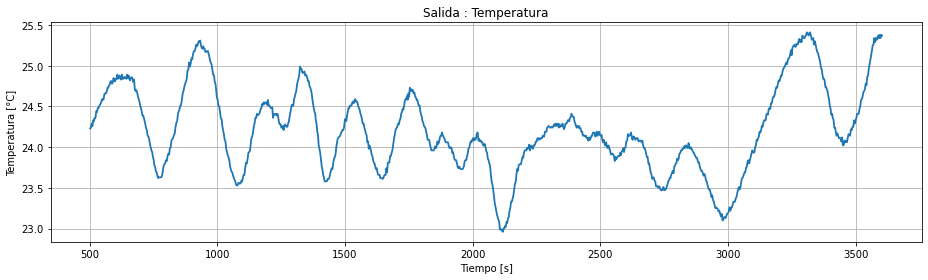
\includegraphics[width=\linewidth]{Figure 2026-07-09 145349.png}
        \caption{Temperatura obtenido con señal multisinusoidal.}
        \label{fig:temperatursisoinvierno}
    \end{subfigure}
    
    \caption{Resultados obtenidos con señal multisinusoidal.}
    \label{fig:resultados_multisinusoidal}
\end{figure}

El análisis de coherencia entre el caudal y la temperatura, Figura \ref{fig:CoherenciaSISOinvierno}, muestra que la relación entre ambas variables depende de la frecuencia. En la zona inferior de la banda se observan valores de coherencia cercanos a 0.4–0.5, seguidos por una disminución pronunciada alrededor de 0.0025 Hz. Posteriormente, la coherencia aumenta de manera progresiva, superando aproximadamente 0.6 a partir de 0.006 Hz y alcanzando valores cercanos a 0.8 hacia 0.01 Hz. Este comportamiento indica que la influencia lineal del caudal sobre la temperatura no se manifiesta con la misma intensidad en toda la banda analizada. En aquellas frecuencias donde la coherencia alcanza valores mayores, las variaciones de la temperatura presentan una relación más consistente con la excitación aplicada al caudal. En cambio, el bajo valor observado alrededor de 0.0025 Hz indica que, en esa región, una menor proporción de la respuesta térmica puede relacionarse directamente con el caudal mediante una relación lineal.



\begin{figure}[H]
    \centering
    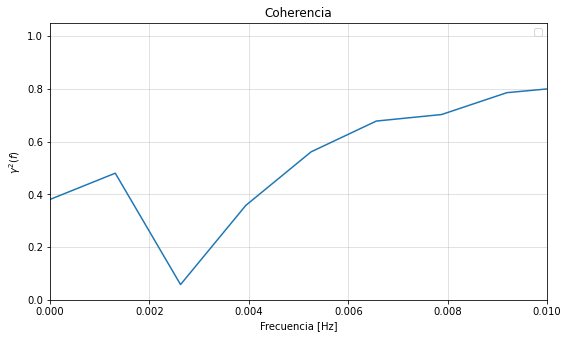
\includegraphics[width=0.5\linewidth]{Figure 2026-08-21 140250 (0).png}
    \caption{Coherencia de la prueba realizada en invierno.}
    \label{fig:CoherenciaSISOinvierno}
\end{figure}
La densidad espectral de potencia de la entrada, Figura \ref{fig:psdSISOinvierno}, muestra que la señal multisinusoidal proporciona contenido energético a lo largo de la banda estudiada. La distribución no es uniforme, observándose niveles relativamente elevados en las frecuencias inferiores y un aumento de la densidad espectral aproximadamente entre 0.004 y 0.007 Hz, seguido posteriormente por una disminución hacia 0.01 Hz. Esto confirma que la señal aplicada introduce excitación en diferentes regiones del intervalo frecuencial considerado. Por su parte, la densidad espectral de potencia de la temperatura, Figura \ref{fig:psdSISOinviernoSalida}, presenta un comportamiento claramente decreciente con el aumento de la frecuencia. La mayor concentración de energía se encuentra en las frecuencias más bajas, mientras que su magnitud disminuye rápidamente a medida que aumenta la frecuencia, alcanzando valores próximos a cero hacia el extremo superior de la banda. Este comportamiento es consistente con la dinámica lenta del sistema térmico, cuya respuesta presenta una mayor contribución de componentes de baja frecuencia y una atenuación progresiva de las variaciones más rápidas.

\begin{figure}[H]
    \centering
    \begin{subfigure}[b]{0.48\textwidth}
        \centering
        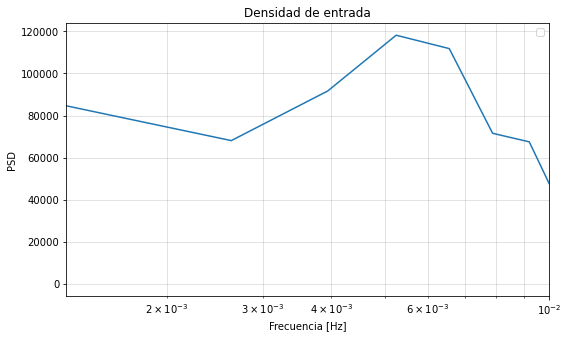
\includegraphics[width=\linewidth]{Figure 2026-08-21 140250 (1).png}
        \caption{Entrada.}
        \label{fig:psdSISOinvierno}
    \end{subfigure}
    \hfill
    \begin{subfigure}[b]{0.48\textwidth}
        \centering
        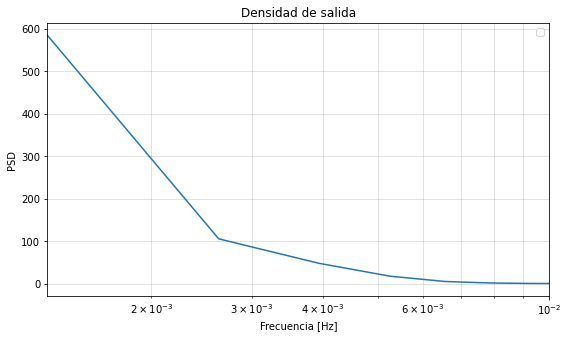
\includegraphics[width=\linewidth]{Figure 2026-08-21 140250 (2).png}
        \caption{Salida.}
        \label{fig:psdSISOinviernoSalida}
    \end{subfigure}
    \caption{Densidad espectral de entrada y salida.}
    \label{fig:psdSISOinvierno_total}
\end{figure}



La magnitud de la FRF (Figura \ref{fig:frfmagnitudSISOinvniero}) presenta, en términos generales, una tendencia decreciente con el aumento de la frecuencia. En la zona inferior de la banda se observan los mayores valores de magnitud, mientras que hacia 0.01 Hz esta disminuye. Aunque existe una variación local en la región intermedia, la tendencia global muestra una atenuación creciente de la respuesta térmica frente a componentes de mayor frecuencia. Este resultado concuerda con lo observado en la densidad espectral de la salida y refleja la limitada capacidad del sistema térmico para responder a variaciones progresivamente más rápidas del caudal. La fase de la función de respuesta en frecuencia (Figura \ref{fig:frfFASEinvinero}) también presenta una evolución dependiente de la frecuencia. Este comportamiento evidencia que el desfase entre las variaciones del caudal y la respuesta térmica cambia con la frecuencia, lo que resulta consistente con la presencia de almacenamiento de energía, inercia térmica y retardos propios de la dinámica del sistema.


\begin{figure}[H]
    \centering
    \begin{subfigure}[b]{0.48\textwidth}
        \centering
        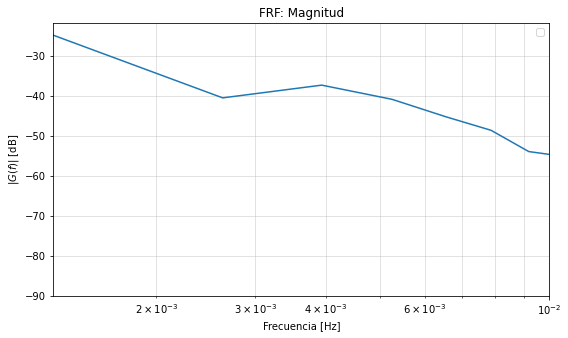
\includegraphics[width=\linewidth]{Figure 2026-08-21 140250 (3).png}
        \caption{Magnitud.}
        \label{fig:frfmagnitudSISOinvniero}
    \end{subfigure}
    \hfill
    \begin{subfigure}[b]{0.48\textwidth}
        \centering
        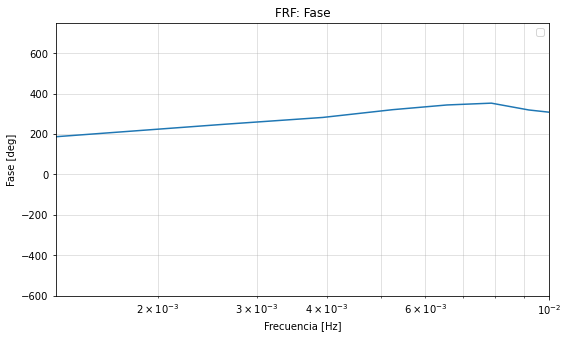
\includegraphics[width=\linewidth]{Figure 2026-08-21 140250 (4).png}
        \caption{Fase.}
        \label{fig:frfFASEinvinero}
    \end{subfigure}
    \caption{Respuesta en frecuencia (FRF): Magnitud y Fase.}
    \label{fig:frf_SISO_invierno}
\end{figure}

En conjunto, el análisis espectral muestra que el ensayo realizado durante el período invernal mantiene una excitación distribuida dentro de la banda de interés, mientras que la respuesta térmica se concentra principalmente en las frecuencias más bajas. La coherencia evidencia que la relación lineal entre caudal y temperatura no es uniforme en toda la banda, presentando una menor consistencia en determinadas frecuencias y aumentando hacia la zona superior del intervalo analizado. Por su parte, la densidad espectral y la función de respuesta en frecuencia muestran una atenuación de la respuesta a medida que aumenta la frecuencia, comportamiento característico de la dinámica lenta del sistema térmico. %Estos resultados permiten caracterizar el comportamiento del sistema bajo las condiciones de operación invernales y establecer las diferencias observadas respecto de los ensayos realizados bajo otras condiciones térmico.



\subsection{Resultados de conjuntos de datos SISO}
A partir del análisis espectral realizado sobre los conjuntos de datos SISO obtenidos con señales PRBS y multisinusoidales, se determinó que las configuraciones evaluadas presentan condiciones adecuadas para analizar la respuesta dinámica del sistema térmico en bajas frecuencias. En particular, las señales aplicadas al caudal permitieron excitar la dinámica dominante del banco de ensayos dentro de la banda de interés, generando una respuesta térmica observable y funciones de respuesta en frecuencia consistentes con el comportamiento esperado de un sistema térmico lento.

En el caso de las señales multisinusoidales, los distintos conjuntos evaluados mostraron una excitación suficiente dentro del rango frecuencial de análisis, una respuesta térmica reproducible y funciones de respuesta en frecuencia comparables entre sí. Esto indica que la variación del número de componentes sinusoidales no modifica de manera significativa la dinámica observada del sistema dentro de la banda de interés. Entre estas configuraciones, la señal multisinusoidal con d = 23 presentó la mayor cobertura frecuencial, al incorporar el mayor número de componentes sinusoidales dentro de la banda considerada. Esta característica permite distribuir la excitación sobre un conjunto más amplio de frecuencias y observar la respuesta del sistema frente a una entrada periódica con contenido espectral definido.

Para la identificación del modelo SISO se seleccionó el conjunto de datos obtenido mediante la señal PRBS con P = 25. Esta elección se fundamenta en que la PRBS proporciona una excitación pseudoaleatoria caracterizada por una sucesión de cambios de nivel que permite explorar la respuesta transitoria del sistema y obtener información dinámica suficiente para el ajuste de los parámetros del modelo. En la configuración seleccionada, el período de reloj de 25 segundos permitió concentrar una parte importante de la excitación en la región de bajas frecuencias, manteniendo además cambios suficientemente espaciados para representar adecuadamente la dinámica lenta del sistema térmico y evitar variaciones excesivamente rápidas en el caudal.

La utilización de una señal distinta para la validación responde a la necesidad de evaluar el modelo con datos que no reproduzcan exactamente las condiciones de excitación empleadas durante la identificación. Por esta razón, se reservó para esta etapa el experimento obtenido mediante una señal multisinusoidal. Su estructura determinista y su distribución de energía en frecuencias específicas permiten comprobar si el modelo identificado a partir de una excitación pseudoaleatoria es capaz de reproducir adecuadamente la respuesta del sistema frente a una entrada con características espectrales diferentes. De este modo, la validación no consiste únicamente en comprobar el ajuste frente a otro registro PRBS, sino en evaluar si la dinámica aprendida por el modelo se mantiene ante una forma de excitación distinta.

Adicionalmente, el conjunto multisinusoidal seleccionado para validación corresponde al ensayo realizado durante el período invernal. Esta condición introduce una diferencia adicional respecto de los datos utilizados para la identificación, ya que las condiciones ambientales, la temperatura inicial del sistema y las pérdidas térmicas hacia el entorno pueden diferir de aquellas presentes durante los ensayos realizados en verano. En consecuencia, este conjunto constituye una condición de validación más exigente, al combinar una señal de entrada diferente con condiciones térmicas de operación distintas.

En consecuencia, se definió una estrategia de identificación y validación basada en conjuntos de datos independientes y con características complementarias. La señal PRBS con P = 25 fue utilizada para la identificación debido a su capacidad para proporcionar una excitación suficientemente rica y adecuada para el ajuste de los parámetros del modelo dentro de la banda dinámica de interés. Por su parte, la señal multisinusoidal fue reservada para la validación debido a que presenta una estructura de excitación distinta y una distribución frecuencial definida, permitiendo comprobar si el modelo conserva su capacidad de representación fuera del conjunto utilizado para su ajuste. El hecho de que este último ensayo haya sido obtenido en invierno añade además una variación en las condiciones de operación, fortaleciendo la evaluación de la capacidad de generalización del modelo SISO.


\section{Modelado y validación}

A partir del análisis realizado sobre los conjuntos de datos experimentales, y una vez comprobado que las señales de excitación empleadas permiten obtener información relevante dentro de la banda de frecuencias de interés, se procede a la etapa de modelación del sistema. En una primera instancia se evaluarán estructuras lineales, seleccionadas de acuerdo con las características dinámicas observadas previamente en la respuesta térmica del banco de ensayos. Posteriormente, el proceso se extendió a estructuras de mayor complejidad, incluyendo modelos con múltiples entradas y modelos no lineales, manteniendo un procedimiento general de identificación y evaluación común.

Antes de realizar la identificación y validación, se excluyen los primeros 500 segundos de cada registro. Este intervalo corresponde al período inicial de estabilización térmica del sistema y, por lo tanto, no se considera representativo de la dinámica que se desea modelar. Como se observa en la evolución temporal de la temperatura de salida de la Figura \ref{fig:temperarturasalida500s}, durante los primeros minutos se produce un incremento pronunciado desde la condición inicial, seguido de una transición hacia un nivel térmico más estable alrededor de los 500 segundos. La inclusión de este tramo introduciría en el conjunto de datos una condición transitoria asociada principalmente al calentamiento inicial del banco, pudiendo afectar la estimación de los parámetros y las métricas de desempeño. Por esta razón, el análisis se realiza a partir de los 500 segundos, considerando desde ese instante la respuesta dinámica del sistema respecto de una condición térmica previamente establecida.


\begin{figure}[H]
    \centering
    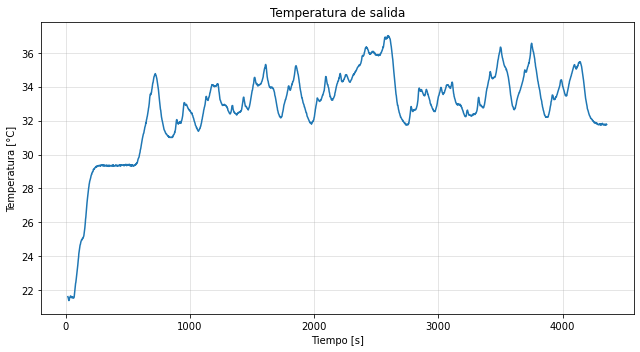
\includegraphics[width=0.5\linewidth]{graficoTEMPERATURA.png}
    \caption{Evolución en el tiempo de la temperatura de salida del sistema.}
    \label{fig:temperarturasalida500s}
\end{figure}



De manera general, el procedimiento empleado para la identificación de los modelos se resume en la Figura \ref{fig:identificacionmodelos}. Este esquema representa una visión global del proceso y es aplicable tanto a las estructuras lineales como a las no lineales consideradas en este trabajo. El proceso comienza con la definición de los datos utilizados para identificación y validación, incluyendo las variables de entrada y salida y su correspondiente preprocesamiento. A partir de estos datos se seleccionan los parámetros asociados a la estructura de cada modelo, tales como órdenes, retardos y coeficientes, cuya naturaleza y cantidad dependen del tipo de estructura evaluada. La selección se realiza considerando criterios como la capacidad de representación, la complejidad del modelo y el costo computacional. Posteriormente, se efectúa la estimación o entrenamiento de los parámetros, obteniéndose un modelo candidato que es evaluado mediante simulación libre. 


\begin{figure}[H]
    \centering
    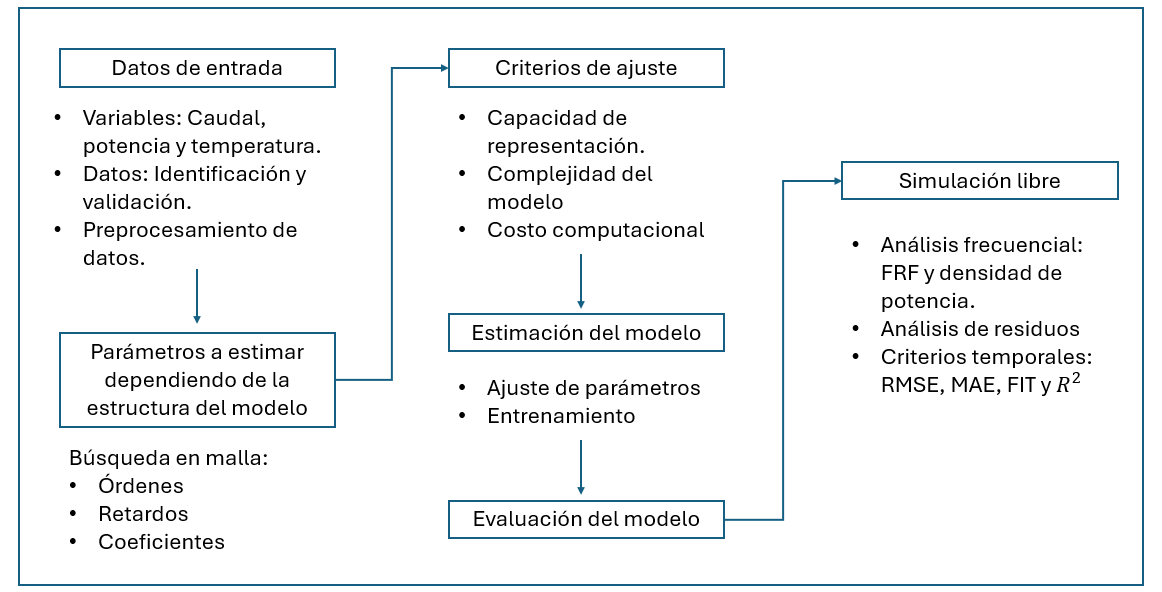
\includegraphics[width=0.7\linewidth]{IDENTIFICACIONMODELOS.png}
    \caption{Proceso de identificación de modelos.}
    \label{fig:identificacionmodelos}
\end{figure}



La evaluación de los modelos se realizará mediante criterios temporales y frecuenciales complementarios. En el dominio del tiempo, las respuestas estimadas serán analizadas en la escala original de las variables, revirtiendo los procesos de normalización o transformación aplicados durante la identificación cuando corresponda. Para cuantificar el desempeño se utilizarán el coeficiente de determinación $R^2$, el error cuadrático medio (RMSE), el porcentaje de ajuste FIT y el error absoluto medio (MAE). $R^2$ y FIT permiten evaluar de manera global la concordancia entre la respuesta medida y la estimada, mientras que RMSE y MAE expresan directamente la magnitud del error en las unidades de la temperatura. La comparación entre modelos se realizará mediante la interpretación conjunta de estos indicadores, evitando basar la selección en una única métrica.
Complementariamente, se analizará la respuesta de los modelos en el dominio de la frecuencia mediante la densidad espectral, la coherencia y la función de respuesta en frecuencia. Estos criterios permiten verificar si el modelo reproduce adecuadamente no solo la trayectoria temporal de la temperatura, sino también la dinámica observada en la banda frecuencial de interés. Esta evaluación es importante, debido a que un modelo puede presentar un error temporal reducido y, al mismo tiempo, no representar correctamente la distribución espectral o la relación dinámica entre la entrada y la salida.


Asimismo, se considerará el análisis de los residuos como parte de la evaluación de cada estructura. En particular, se examinará su comportamiento y su correlación con las señales de entrada, con el propósito de determinar si permanece información dinámica de la excitación que no haya sido capturada por el modelo. La presencia de correlaciones significativas puede indicar que parte de la relación entre la entrada y la salida todavía no ha sido representada adecuadamente.

Todos los modelos serán evaluados mediante simulación libre. En esta modalidad, el modelo genera la evolución completa de la salida a partir de las señales de entrada conocidas y de sus propias salidas calculadas en instantes anteriores. Una vez establecidas las condiciones iniciales necesarias para iniciar la simulación, el modelo avanza de manera recursiva en el tiempo: en cada instante calcula una nueva temperatura utilizando las entradas correspondientes y, cuando la estructura lo requiere, las salidas estimadas previamente por el propio modelo. De esta forma, cualquier error cometido en un instante puede propagarse hacia los siguientes pasos de simulación. La simulación libre resulta pertinente para el sistema térmico estudiado debido a su inercia y a la presencia de retardos. Estas características hacen que la respuesta actual dependa de la evolución previa del sistema, por lo que la capacidad del modelo para mantener una trayectoria estable y representativa sin utilizar continuamente la temperatura real constituye una exigencia relevante. Bajo estas condiciones, pequeños errores pueden acumularse progresivamente a medida que avanza la simulación, de modo que reproducir adecuadamente la evolución de la temperatura durante períodos prolongados permite evaluar no solo el ajuste instantáneo del modelo, sino también su capacidad para representar la dinámica global del sistema.

En consecuencia, la selección de las estructuras se realizará considerando simultáneamente su precisión temporal, la independencia de los residuos y la consistencia de su comportamiento frecuencial. Este enfoque permite evaluar no solo qué tan próximo se encuentra el modelo de los datos medidos, sino también si reproduce de manera adecuada la dinámica dominante del sistema térmico dentro del rango de operación estudiado.



\subsection{Modelo ARX}

A partir del análisis de los datos experimentales no fue posible establecer de manera concluyente que el sistema presente un comportamiento lineal e invariante en el tiempo en toda la banda de interés. Sin embargo, las relaciones observadas entre la entrada de caudal y la respuesta térmica permiten considerar el uso de modelos lineales como una primera aproximación para representar la dinámica del sistema. Este enfoque permite disponer de una referencia inicial de baja complejidad y evaluar posteriormente si estructuras más elaboradas resultan necesarias para capturar los efectos dinámicos que no sean adecuadamente representados.

Como primera estructura se seleccionó un modelo ARX (AutoRegressive with eXogenous inputs, o modelo autorregresivo con entradas exógenas), ampliamente utilizado en identificación de sistemas por su formulación sencilla y su reducido costo computacional. Este tipo de modelo representa la salida actual a partir de valores pasados de la propia salida y de la entrada exógena, permitiendo capturar relaciones dinámicas lineales entre ambas variables.

La elección del modelo ARX como punto de partida se fundamenta principalmente en su simplicidad estructural y en la facilidad de estimación de sus parámetros, los cuales pueden obtenerse mediante métodos lineales de mínimos cuadrados sin recurrir a procedimientos iterativos complejos. De esta forma, el modelo ARX constituye una referencia adecuada para evaluar hasta qué punto una estructura lineal es capaz de representar la dinámica observada y establecer una base de comparación para modelos posteriores de mayor complejidad.




\subsection{Proceso de identificación y selección para modelos ARX}


El proceso de identificación se desarrolló mediante una exploración sistemática de diferentes estructuras ARX, con el objetivo de seleccionar una combinación de órdenes capaz de representar la dinámica observada sin introducir una complejidad innecesaria. Para ello, se consideraron conjuntamente el desempeño temporal del modelo, su capacidad de simulación, la estabilidad de la estructura identificada y las propiedades estadísticas de los residuos. El procedimiento aplicado se describe a continuación.


\begin{enumerate}
    \item \textbf{División de los datos para la identificación y validación}

    El conjunto de datos disponible se dividió cronológicamente en dos subconjuntos independientes. El 80 \% inicial de los registros se utilizó para estimar los parámetros de cada estructura candidata, mientras que el 20 \% restante se reservó para evaluar su comportamiento frente a datos no utilizados durante el ajuste. Esta separación permite analizar la capacidad de generalización de cada modelo y evitar que la selección se base exclusivamente en su desempeño sobre los datos empleados durante la estimación. En el procedimiento implementado, esta división se realiza antes de estimar los parámetros de preprocesamiento.

    

    \item \textbf{Preprocesamiento de las variables}

    Antes de la identificación, las señales de entrada y salida fueron sometidas a eliminación de tendencia y normalización. Los parámetros empleados para estas transformaciones se determinaron utilizando únicamente el conjunto destinado a identificación y posteriormente se aplicaron tanto a los datos de identificación como a los de validación. De esta forma, se evita utilizar información procedente del conjunto de validación durante la etapa de ajuste. La eliminación de tendencia permite reducir la influencia de variaciones lentas no asociadas directamente con la dinámica que se desea representar, mientras que la normalización lleva las variables a escalas comparables y mejora las condiciones numéricas de la estimación.

    \item \textbf{Definición de las estructuras ARX candidatas}

    Cada modelo ARX queda determinado por tres órdenes: $n_{a}$, $n_{b}$ y $n_{k}$. El parámetro $n_{a}$ establece el número de valores pasados de la salida utilizados por el modelo, $n_{b}$ determina la cantidad de valores pasados de la entrada considerados y $n_{k}$ representa el retardo discreto entre una modificación del caudal y el momento en que esta comienza a influir sobre la temperatura.

    En lugar de seleccionar estos órdenes de manera arbitraria, se definió una malla de combinaciones posibles de $n_{a}$, $n_{b}$ y $n_{k}$. Para esta primera exploración se utilizaron rangos acotados, suficientes para evaluar estructuras de distinta complejidad sin generar un número excesivo de modelos candidatos. En cada combinación de órdenes de $n_{a}$, $n_{b}$ y $n_{k}$ se construyó la matriz de regresores, la cual reúne los valores pasados de la salida y de la entrada utilizados para estimar la salida actual del modelo. Debido a que su construcción depende directamente de los órdenes seleccionados, se verificó que cada combinación dispusiera de un número suficiente de muestras para realizar una estimación confiable. Las configuraciones que no cumplían esta condición fueron descartadas antes del proceso de identificación.
    \item \textbf{Estimación de parámetros}

    Para cada combinación admisible de $n_{a}$, $n_{b}$ y $n_{k}$ se realizó la correspondiente matriz de regresión. A partir de esta matriz se estimaron los coeficientes autorregresivos y los coeficientes asociados al caudal mediante un procedimiento de mínimos cuadrados. Este procedimiento determina los parámetros que minimizan la suma de los errores cuadráticos entre la salida medida y la salida estimada por el modelo sobre el conjunto de identificación. Debido a que el modelo ARX es lineal respecto de sus parámetros, este procedimiento permite obtenerlos de manera directa y con un bajo costo computacional.
    
    \item \textbf{Evaluación mediante simulación}
    
    Una vez estimados los parámetros de cada estructura, el modelo fue evaluado mediante simulación. En esta modalidad, las salidas calculadas previamente por el propio modelo son utilizadas para continuar generando la trayectoria futura, en lugar de sustituirlas continuamente por los valores reales de temperatura. De esta manera se evalúa la capacidad de la estructura identificada para reproducir de forma autónoma la evolución dinámica del sistema. El mismo modelo se simuló sobre el conjunto utilizado para identificación y sobre el segmento reservado para validación. De esta forma, fue posible comparar su desempeño tanto sobre los datos utilizados para el ajuste como sobre datos no empleados durante la estimación.

    El desempeño temporal de cada candidato se cuantificó mediante RMSE y FIT. Se otorgó especial importancia al comportamiento sobre el conjunto de validación, dado que este segmento no participa en la estimación de los parámetros.

    \item \textbf{Análisis de los residuos}

    El error entre la salida medida y la respuesta simulada fue utilizado para evaluar si permanecía información dinámica sin representar. Para ello, se analizó la autocorrelación de los residuos y la correlación cruzada entre los residuos y la entrada de caudal. Un modelo adecuado debería generar residuos con baja autocorrelación para retardos distintos de cero, ya que una estructura persistente en el error indicaría la existencia de dinámica que el modelo no logró capturar. De manera similar, una correlación significativa entre los residuos y la entrada sugeriría que todavía existe información asociada al caudal que podría ser utilizada para mejorar la representación del sistema. Estas propiedades fueron incorporadas al procedimiento de selección mediante términos de penalización.
    
    \item \textbf{Evaluación de estabilidad y complejidad}
    
    Además del ajuste obtenido, se evaluó la estabilidad dinámica de cada modelo ARX. Para ello, se calcularon las raíces del polinomio autorregresivo, ya que su ubicación determina si la respuesta del modelo permanece acotada o puede crecer de manera no controlada durante la simulación. En un sistema discreto estable, todas estas raíces deben encontrarse dentro del círculo unitario del plano complejo, es decir, deben tener módulo menor que uno. Cuando alguna raíz se encuentra sobre o fuera de este límite, la estructura puede generar una respuesta inestable, por lo que dichos modelos fueron descartados o fuertemente penalizados dentro del proceso de selección.

Por otra parte, se utilizó el criterio de información bayesiano (BIC) para considerar la complejidad de cada estructura. Este criterio combina la calidad del ajuste con el número de parámetros empleados, penalizando aquellos modelos que aumentan su complejidad sin producir una mejora suficientemente significativa en la representación de los datos. De esta manera, el BIC permite evitar la selección de modelos excesivamente parametrizados y favorece estructuras más parsimoniosas. Por lo tanto, entre modelos con desempeños similares, se prioriza aquel que logra representar adecuadamente la dinámica utilizando una menor cantidad de parámetros.

    
    \item \textbf{Selección mediante un criterio global}
    
    Debido a que ningún indicador individual permite evaluar completamente la calidad de un modelo dinámico, las estructuras candidatas fueron ordenadas mediante una función de costo que considera simultáneamente su desempeño en validación, el error de simulación, la complejidad, las propiedades de los residuos y la estabilidad. De esta manera, la selección no corresponde necesariamente al modelo con el menor RMSE o el mayor FIT de manera aislada, sino a la estructura que presenta el mejor equilibrio entre precisión, capacidad de generalización, complejidad y consistencia dinámica.



    \item \textbf{Evaluación final del modelo seleccionado}

    Una vez determinada la combinación óptima de $n_{a}$, $n_{b}$ y $n_{k}$ se reconstruyó la respuesta del modelo en las unidades físicas originales, revirtiendo las transformaciones realizadas durante el preprocesamiento. Sobre esta respuesta se calcularon los indicadores finales de desempeño, incluyendo $R^2$, RMSE, FIT y MAE. Además, se inspeccionaron la respuesta temporal y los residuos obtenidos, de manera de complementar los indicadores numéricos con una evaluación de la capacidad del modelo para seguir la evolución de la temperatura.


    
\end{enumerate}
\begin{comment}
    
   
\subsection{Primer modelo ARX}
Según la identificación, el mejor modelo identificado corresponde a:
\begin{itemize}
    \item $n_{a}=4$
    \item $n_{b}=4$
    \item $n_{k}=5$ 
\end{itemize}
Así, junto con los coeficientes, la estructura del modelo obtenido se expresa como:

$$y_k =0.6454y(k-1) + 1.1672y(k-2) - 0.5971y(k-3)  -0.2207y(k-4) $$
$$- 0.0006126u(k-5) - 0.0018659u(k-6)-0.0053774u(k-7)+0.0008745u(k-8)$$
\end{comment} 
\begin{comment}
    

%$$y_{k}=0,6454y(k-1)+1,1672y(k-2)-0,5971y(k-3)-0,2207y(k-4)-0,0006126u(k-5)-0,0018659u(k-6)-0,0053774u(k-7)+0,0008745u(k-8)$$

La validación del modelo realiza en la identificación de este entrega los siguientes indicadores temporales:
\begin{itemize}
    \item RMSE = 1.1988 °C
    \item R² = 0.8241
    \item FIT= 58.06\%
\end{itemize}

En la Figura \ref{fig:primermodelo} se observa el comportamiento de este primer modelo en esta misma validación:

\begin{figure}[H]
    \centering
    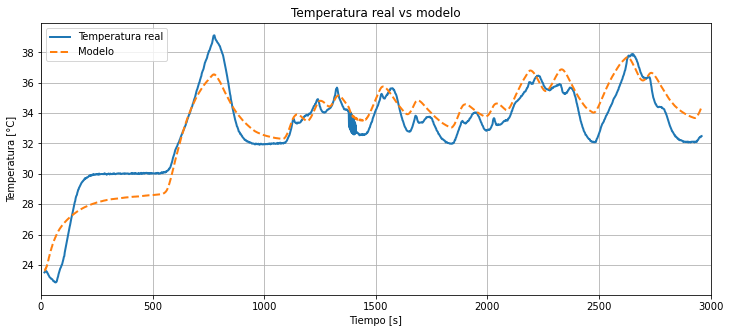
\includegraphics[width=0.7\linewidth]{ModeloARXprbs.png}
    \caption{Comportamiento de primer modelo ARX.}
    \label{fig:primermodelo}
\end{figure}

\subsubsection{Validación}
La validación del modelo en tiempo real se realizó mediante datos diferentes a los utilizados en el entrenamiento, pues aquí se observó el comportamiento del modelo al excitar al sistema con una señal multisinusoidal (Figura \ref{fig:ValidacionprimermodeloARX}).

\begin{figure}[H]
    \centering
    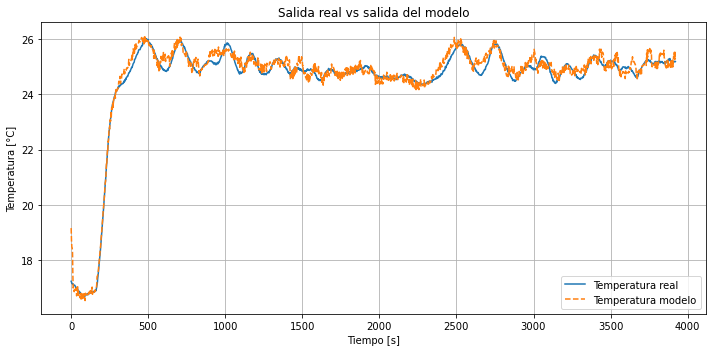
\includegraphics[width=0.65\linewidth]{Figure 2026-05-13 222242 (0).png}
    \caption{Validación en tiempo real del primer modelo ARX}
    \label{fig:ValidacionprimermodeloARX}
\end{figure}

En el gráfico, en color naranjo se observa el comportamiento del modelo con respecto a la temperatura real del sistema, donde se identifica que este sí logra seguir la tendencia global del sistema. Se muestra que el modelo reproduce adecuadamente el transitorio inicial, la variaciones lentas y las oscilaciones principales del sistema.
Los indicadores temporales obtenidos son:
\begin{itemize}
    \item RMSE: 0.229258 °C
    \item MAE: 0.174116 °C
    \item FIT: 87.757 \%
    \item R²: 0.985011
    
\end{itemize}




El resultado del RMSE indica que el error cuadrático medio del modelo es inferior a un cuarto de grado Celsius y el MAE muestra un error absoluto promedio bajo, lo que se considera aceptable según la dinámica térmica lenta, el ruido experimental, la incertidumbre instrumental y las variaciones reales del sistema.
El valor del FIT indica que el modelo reproduce en más de un 87\% la variabilidad dinámica observada experimentalmente.
El coeficiente $R^2$ señala que aproximadamente el 98.5\% de la variabilidad de la temperatura medida es explicada por el modelo.


Autocorrelación y correlación entrada-residuo

Si bien, el gráfico siguiente (Figura \ref{fig:residuosARX1}) muestra que los residuos del modelo son pequeños, estos deberían ser aleatorios, sin estructura temporal y no estar correlacionados con la entrada, es decir, comportarse como ruido blanco \cite{ljung1999system}. Sin embargo, se observa que permanece varios segundos con una tendencia similar, sin comportamiento aleatorio.

\begin{figure}[H]
    \centering
    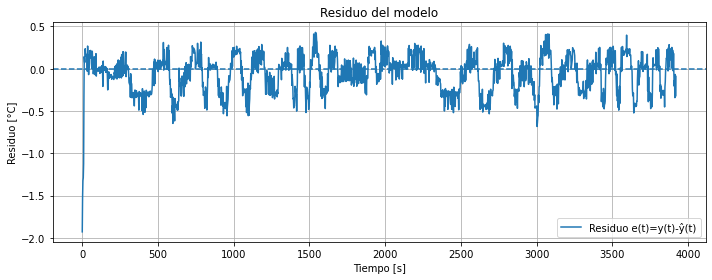
\includegraphics[width=0.65\linewidth]{Figure 2026-05-13 222242 (1).png}
    \caption{Residuos del modelo.}
    \label{fig:residuosARX1}
\end{figure}


La Figura \ref{fig:Correlacionentradaresiduo} corresponde a la correlación cruzada entre la entrada del sistema y el residuo del modelo. Este análisis forma parte de la validación residual descrita por Ljung \cite{ljung1999system} y también por Tangilara \cite{tangirala2018principles}, quienes establecen que un buen modelo debe generar residuos independientes de entradas pasadas.
El objetivo de la correlación entrada-residuo es verificar si aún existe información de la entrada contenida en el error del modelo. Según el criterio descrito por \cite{ljung1999system} y \cite{tangirala2018principles}, si el modelo representa adecuadamente la dinámica entrada-salida del sistema, entonces el residuo no debería presentar correlación significativa con entradas pasadas.
La correlación cruzada puede expresarse como: $R(\tau)=E[u(k)e(k-\tau)]$, donde $\tau$ corresponde al lag o retardo. Este representa el desplazamiento temporal aplicado a una de las señales para evaluar dependencias entre valores presentes y pasados. En sistemas dinámicos esto es fundamental, ya que la respuesta física del sistema no ocurre instantáneamente. En sistemas térmicos, los efectos del caudal sobre la temperatura aparecen después de cierto tiempo debido a fenómenos de acumulación e inercia térmica.
La correlación presentada en el eje vertical se encuentra normalizada, por lo que los valores quedan acotados aproximadamente entre -1 y 1. 
En un modelo bien identificado la correlación entrada-residuo debería permanecer cercana a cero para todos los retardos distintos de cero, pues toda la información asociada a la entrada debió haber sido capturada por el modelo, dejando el en residuo únicamente perturbaciones impredecibles o ruido \cite{ljung1999system} y \cite{tangirala2018principles}.
El gráfico muestra una estructura altamente organizada y persistente, con valores cercanos a 0.9 alrededor de lag cero y amplias regiones con correlaciones significativamente distintas de cero. Su forma suave y triangular evidencia que el residuo no posee un comportamiento aleatorio.
Las correlaciones elevadas alrededor de lag cero indican que el error del modelo aún está fuertemente relacionado con variaciones en la entrada. Es decir, cambios en el caudal siguen reflejándose parcialmente en el residuo, lo que evidencia que el modelo no logra representar completamente la dinámica entrada-salida del sistema. Asimismo, las regiones negativas observadas siguieren la existencia de dinámicas más complejas asociadas a retardos térmicos, acumulación de energía o fenómenos dinámicos no representados por el modelo identificado.

\begin{figure}[H]
    \centering
    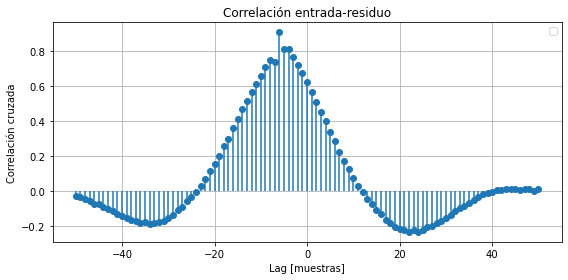
\includegraphics[width=0.5\linewidth]{Correlación entrada salida modelo.png}
    \caption{Correlación entre la entrada del sistema y residuos.}
    \label{fig:Correlacionentradaresiduo}
\end{figure}
La PSD (Figura \ref{fig:PSDmodeloARX} ) muestra que la señal de entrada presenta suficiente contenido energético en bajas frecuencias, permitiendo una excitación adecuada de la dinámica dominante del sistema. Asimismo, la similitud observada entre la PSD de la salida real y de la salida estimada por el modelo indica que  este logra reproducir el comportamiento dinámico de baja frecuencia. No obstante, se observan diferencias hacia frecuencias cercanas al límite superior de la banda analizada, lo que sugiere la existencia de dinámicas adicionales no completamente representadas por el modelo.

\begin{figure}[H]
    \centering
    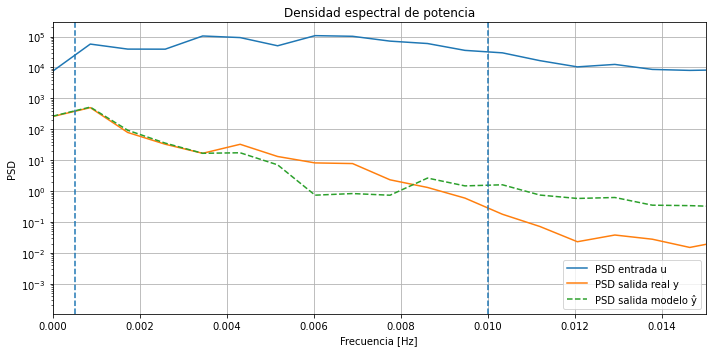
\includegraphics[width=0.65\linewidth]{PSD frecuencia importante.png}
    \caption{Densidad espectral en la banda de interés.}
    \label{fig:PSDmodeloARX}
\end{figure}

La Figura \ref{fig:comparacion_frfSISO} muestra la comparación entre la respuesta en frecuencia del sistema real y la respuesta en frecuencia del modelo identificado. La FRF (Frecuency Response Function) describe la relación entre la entrada y salida en el dominio de la frecuencia, indicando cuánto cambia la temperatura frente a oscilaciones de caudal y cuánto desfase temporal existe para cada frecuencia.
La magnitud de la FRF representa cuánto responde la temperatura frente a una oscilación del caudal en cierta frecuencia. En este caso, se observa que la FRF real y la FRF del modelo son bastante similares en frecuencias bajas, obteniendo que el modelo representa razonablemente la dinámica principal y capturando adecuadamente la respuesta lenta del sistema.
La fase de la FRF cuantifica el retraso dinámico y en el gráfico se ve que la fase del modelo sigue de buena manera la fase real en gran parte de la banda de interés, lo que significa que el modelo logra representar retardos dinámicos.
Las diferencias de ambas FRFs especialmente en frecuencias más altas podría reflejar ruido experimental, dinámica no modelada o incertidumbre espectral.




\begin{figure}[H]
    \centering
    \begin{subfigure}[b]{0.7\linewidth}
     \centering
     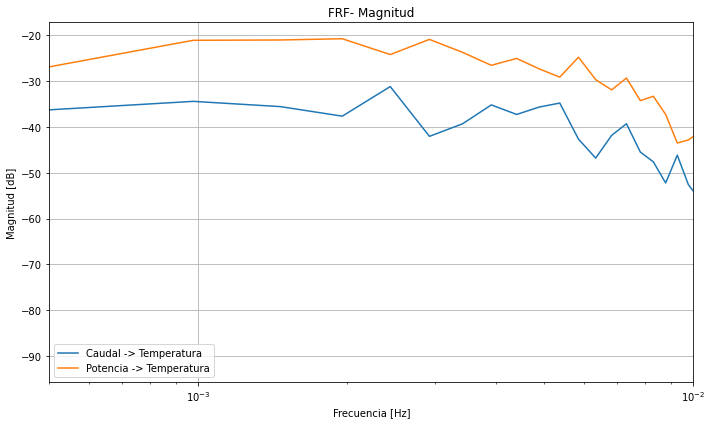
\includegraphics[width=0.5\linewidth]{FRFmagnitud.png}
     \caption{FRF magnitud.}
     \label{fig:FRFmagnitud}
    \end{subfigure}
    \begin{subfigure}[b]{0.7\linewidth}
     \centering
     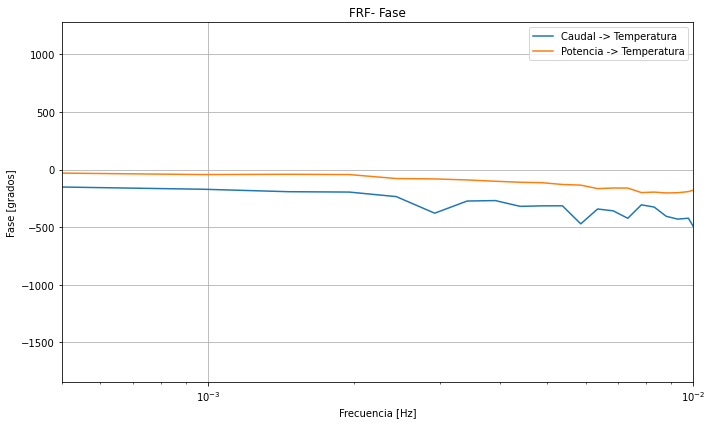
\includegraphics[width=0.5\linewidth]{FRFfase.png}
     \caption{FRF fase.}
     \label{fig:FRFfase}
    \end{subfigure}
    \caption{Comparación entre la respuesta en frecuencia del sistema y el modelo.}
    \label{fig:comparacion_frfSISO}
\end{figure}

Los resultados obtenidos muestran que este primer modelo ARX identificado logra reproducir adecuadamente la dinámica dominante del sistema de emulación termosolar, presentando un buen ajuste temporal, bajos errores de predicción y una alta concordancia entre la salida medida y la salida estimada. Asimismo, el análisis frecuencias mediante PSD y FRF evidencia que el modelo representa razonablemente bien el comportamiento dinámico de baja frecuencia, reproduciendo de buena forma la dinámica dominante dentro de la banda de interés.
Sin embargo, el análisis revela correlación entre la entrada y el residuo, habiendo entonces componentes dinámicas remanentes no representadas por el modelo. Las diferencias observadas en ciertas regiones frecuenciales de la FRF refuerzan esta conclusión, sugiriendo la existencia de dinámicas adicionales asociadas a fenómenos térmicos complejos o efectos no lineales presentes en el sistema experimental.
En consecuencia, este modelo puede considerarse adecuado para representar la dinámica dominante y el comportamiento global del sistema en la banda de interés analizada, aunque no constituye una representación completa de toda la dinámica física presente en el proceso real.


\end{comment}





\subsection{Primer modelo ARX: Exploración}

Como primera aproximación al modelado SISO se desarrolló un modelo ARX de carácter exploratorio utilizando el conjunto de datos seleccionado para la identificación. El propósito de esta etapa no fue establecer inmediatamente una representación definitiva del sistema, sino evaluar la capacidad inicial de una estructura ARX para reproducir la dinámica térmica, comprobar el procedimiento de búsqueda de órdenes y detectar posibles limitaciones que orientaran las etapas posteriores de modelación.

En esta primera exploración se trabajó directamente con la temperatura de salida, previa aplicación de los procedimientos de preprocesamiento definidos anteriormente. A partir de una malla inicial de estructuras candidatas se evaluaron distintas combinaciones de los órdenes $n_{a}$, $n_{b}$ y $n_{k}$. Dentro del espacio de búsqueda considerado, la estructura que presentó el mejor compromiso según los criterios establecidos correspondió a:


\begin{itemize}
    \item $n_{a}=17$
    \item $n_{b}=21$
    \item $n_{k}=9$ 
\end{itemize}

Estos valores no fueron establecidos previamente a partir de parámetros físicos del banco de ensayos, sino que corresponden al resultado del proceso de selección realizado sobre las estructuras evaluadas. Por lo tanto, su interpretación debe entenderse principalmente desde la formulación matemática del modelo ARX y no como una determinación directa de constantes físicas del sistema.


El orden $n_{a}=17$ indica que el cálculo de la salida actual utiliza las 17 muestras anteriores de la temperatura. Considerando un tiempo de muestreo de 2 segundos, la estructura incorpora información de la evolución de la salida correspondiente a los 34 s anteriores. Este orden determina la extensión de la historia de la salida considerada por la parte autorregresiva del modelo. Sin embargo, estos 34 s no deben interpretarse directamente como una constante de tiempo física, sino como el horizonte de información pasada que resultó seleccionado para representar la dinámica dentro de la estructura ARX evaluada.

Por su parte, $n_{b}=21$ establece que el modelo utiliza 21 muestras de la entrada de caudal para calcular la temperatura actual. Estas muestras no comienzan en el instante inmediatamente anterior, sino que se encuentran desplazadas por el retardo definido mediante $n_k$. En consecuencia, $n_b$ determina la extensión de la historia de la entrada considerada por el modelo y permite representar cómo las variaciones anteriores del caudal contribuyen a la respuesta térmica.

Finalmente, $n_k=9$ representa el retardo discreto incorporado entre la entrada y la salida. Debido a que el período de muestreo es de 2 segundos, este valor corresponde a un retardo modelado de 18 segundos. Así, el primer término de entrada considerado corresponde a $u(k-9)$. Como $n_b=21$, la estructura utiliza posteriormente los términos hasta $u(k-29)$, por lo que la información del caudal incluida en el modelo abarca retardos comprendidos entre aproximadamente 18 y 58 segundos respecto de la salida que se desea calcular. El valor de $n_k$ debe interpretarse como el retardo seleccionado por el proceso de identificación para representar la relación entrada-salida y no necesariamente como una medición directa del tiempo de transporte físico del sistema.

La combinación $n_a=17$, $n_b=21$ y $n_k=9$ da lugar, por tanto, a una estructura de orden relativamente elevado. Esto indica que, dentro de la malla explorada, el procedimiento necesitó considerar una cantidad importante de información histórica de la entrada y de la salida para mejorar la representación de los datos. Sin embargo, una mayor cantidad de parámetros no garantiza por sí misma una representación adecuada del sistema, especialmente cuando el modelo se utiliza en simulación libre. Por esta razón, la estructura seleccionada en esta etapa debe considerarse una primera referencia cuya validez será determinada a partir de los resultados de validación.



La ecuación lineal obtenida para el modelo se presenta a continuación. En ella, la salida actual depende de una combinación lineal de salidas pasadas y entradas retardadas, de acuerdo con la estructura característica de un modelo ARX.


$$y_(k)= 0.5429y(k−1)+1.1178y(k−2)−0.4487y(k−3)−0.1135y(k−4)$$ 
$$−0.1296y(k−5)+0.0082y(k−6)+0.0542y(k−7)−0.0125y(k−8) $$
$$−0.0198y(k−9)−0.0220y(k−10)+0.0991y(k−11)−0.0006y(k−12) $$
$$−0.0893y(k−13)−0.0189y(k−14)+0.0001y(k−15)−0.0311y(k−16) $$
$$+0.0543y(k−17)−0.0317u(k−9)−0.0133u(k−10)+0.0009u(k−11)$$
$$+0.0194u(k−12)+0.0236u(k−13)−0.0015u(k−14)−0.0044u(k−15)$$
$$−0.0043u(k−16)+0.0021u(k−17)−0.0027u(k−18)−0.0021u(k−19)$$
$$+0.0015u(k−20)+0.0064u(k−21)−0.0004u(k−22)+0.00004u(k−23)$$ 
$$−0.0060u(k−24)+0.0066u(k−25)−0.0017u(k−26)+0.0035u(k−27)$$
$$+0.0039u(k−28)  −0.0189u(k−29)$$

\begin{comment}
    

En la Figura \ref{fig:modeloARX2} se presenta la comparación entre la salida real del sistema y la respuesta estimada por el segundo modelo ARX identificado. Se observa que el modelo logra reproducir adecuadamente la tendencia general y la dinámica dominante del sistema térmico, aunque aún existen diferencias locales asociadas a fenómenos no modelados, ruido de medición y posibles no linealidades presentes en el proceso real.

\begin{figure}[H]
    \centering
    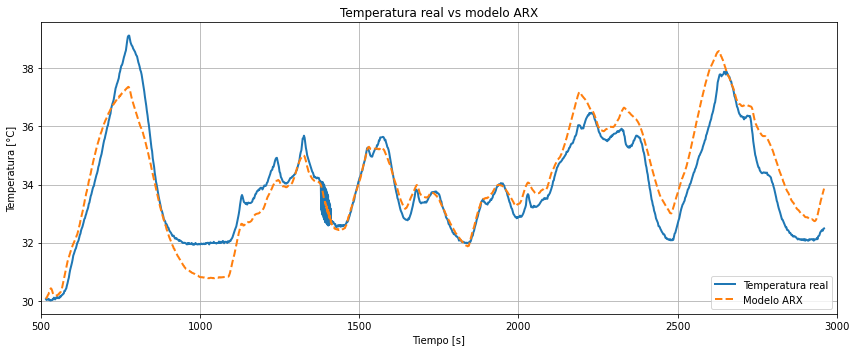
\includegraphics[width=0.5\linewidth]{Grafico arx 2 identificacion.png}
    \caption{Segundo modelo ARX y su comportamiento.}
    \label{fig:modeloARX2}
\end{figure}

\subsubsection{Validación}

La validación en tiempo real de este segundo modelo se realizó de la misma forma que la validación del primer modelo ARX. Se excito al sistema con una señal multisinuosidal, diferente a la utilizada en la recolección de los datos de identificación.
En la Figura \ref{fig:ValidacionARX2} se observa el comportamiento del segundo modelo ARX identificado, el cual muestra una alta concordancia entre la temperatura real y la temperatura estimada. Visualmente, el gráfico es uniforme durante casi uniforme durante todo el experimento.
\begin{figure}[H]
    \centering
    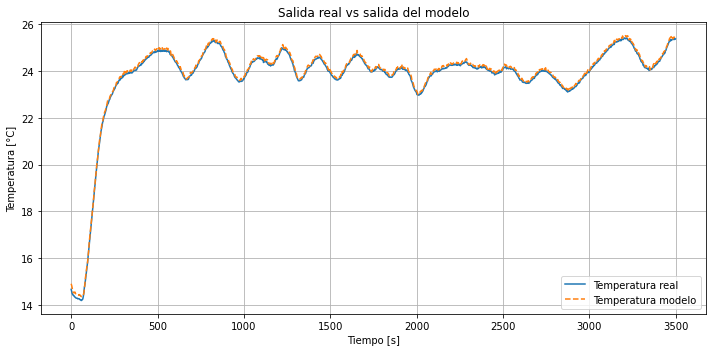
\includegraphics[width=0.65\linewidth]{Figure 2026-05-14 215932 (0).png}
    \caption{Temperatura real comparada con la temperatura simulada por el modelo.}
    \label{fig:ValidacionARX2}
\end{figure}

Los indicadores temporal muestran un alto desempeño:
\begin{itemize}
    \item RMSE: 0.091180 °C. Este valor significa que el error cuadrático medio entre la temperatura real y la temperatura estimada es inferior a una décima de grado Celsius. Por lo que el modelo reproduce bien la temperatura medida.
    \item MAE: 0.082384 °C. En promedio, el modelo se equivoca casi 0.08°C.
    \item FIT: 95.104 \%. El resultado indica que este nuevo modelo reproduce más del 95\% de la variabilidad dinámica observada en la señal de temperatura.
    \item R²: 0.997603. Es decir, el 99.76\% de la variabilidad de la temperatura medida es explicada por el modelo.   
\end{itemize}

El gráfico de residuos (Figura \ref{fig:residuosARX2}) muestra que la variación entre la temperatura real y la temperatura estimada por el modelo es bastante más pequeña que la observada por el modelo anterior. Además, los residuos no presentan una estructura dinámica claramente definida ni tendencias visibles, indicando que el modelo logra capturar gran parte de la dinámica del sistema \cite{ljung1999system}. 
\begin{figure}[H]
    \centering
    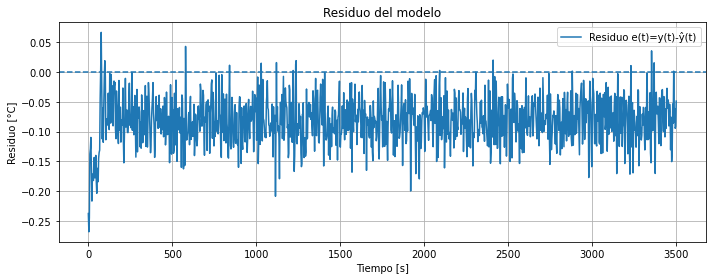
\includegraphics[width=0.65\linewidth]{Figure 2026-05-14 215932 (1).png}
    \caption{Residuos del segundo modelo ARX.}
    \label{fig:residuosARX2}
\end{figure}

 La correlación entre la entrada del sistema y el residuo (Figura \ref{fig:correlacionentradasalidaARX2}) muestra una reducción significativa de las correlaciones respecto al modelo anterior, indicando que el modelo identificado logra representar gran parte de la dinámica entrada-salida del sistema. Las correlaciones observadas presentan amplitudes relativamente pequeñas y considerablemente más cercanas a cero, en comparación al modelo anterior. Sin embargo, aún se muestran ciertas estructuras organizadas y correlaciones persistentes para algunos retardos, lo que sugiere la existencia de dinámicas no completamente representadas por el modelo.

 \begin{figure}[H]
     \centering
     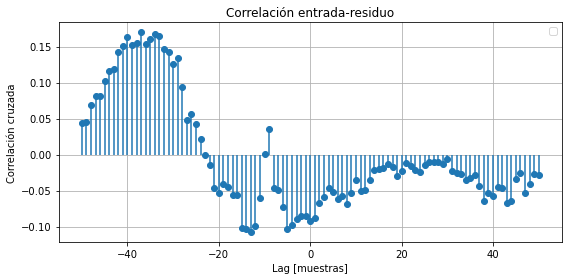
\includegraphics[width=0.5\linewidth]{Figure 2026-05-14 215932 (4).png}
     \caption{Correlación entre la entrada y la salida simulada.}
     \label{fig:correlacionentradasalidaARX2}
 \end{figure}

De la Figura \ref{fig:PSDARX2} se observa que la densidad espectral de la salida real y la salida del modelo coinciden prácticamente en toda la banda de interés, lo que implica una reproducción correcta de la energía espectral por parte del modelo, una buena representación de la dinámica lenta del sistema y la adecuada captura de las frecuencias dominantes.
\begin{figure}[H]
    \centering
    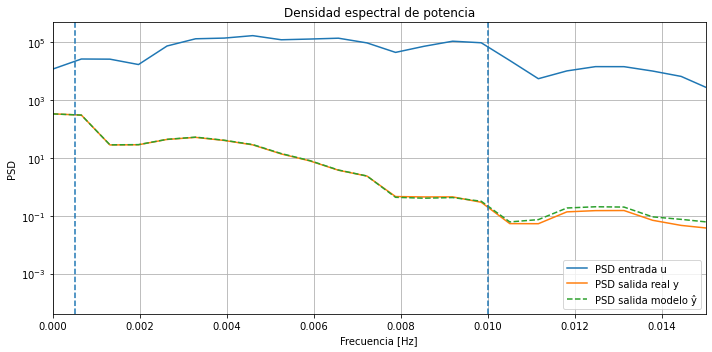
\includegraphics[width=0.5\linewidth]{Figure 2026-05-14 215932 (5).png}
    \caption{Densidad espectral de entrada, salida real y salida simulada.}
    \label{fig:PSDARX2}
\end{figure}


El análisis de los gráficos de la FRF de magnitud y fase (Figura \ref{fig:comparacion_frf}) resulta en que ambos coinciden con la FRF real en toda la banda de frecuencias de interés. Por lo tanto, el modelo reproduce adecuadamente la ganancia dinámica y los retardos y desfases térmicos.

\begin{figure}[H]
    \centering
    \begin{subfigure}{0.48\linewidth}
      \centering
      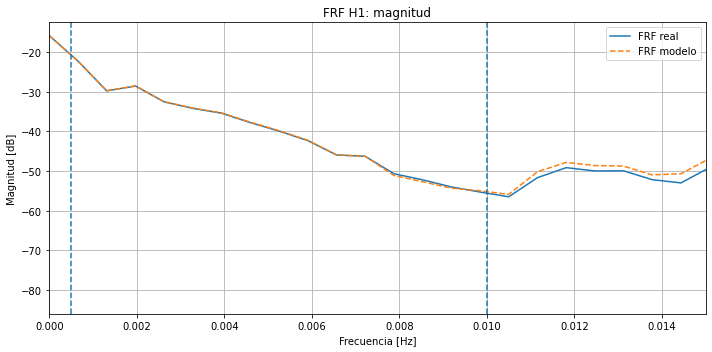
\includegraphics[width=\textwidth]{Figure 2026-05-14 215932 (7).png}
      \caption{Magnitud de la FRF del segundo modelo ARX.}
      \label{fig:FRFmagnitudARX2}
    \end{subfigure}
    \hfill 
    \begin{subfigure}{0.48\linewidth}
      \centering
      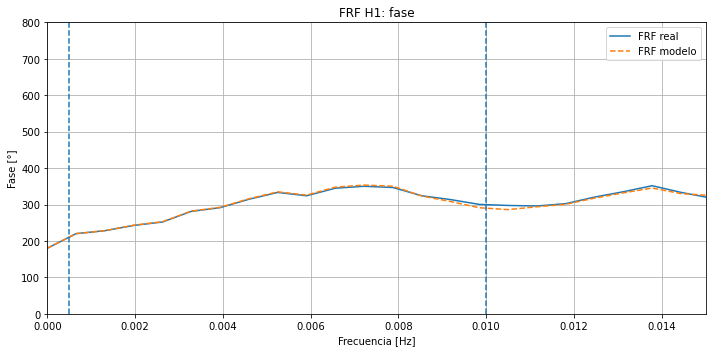
\includegraphics[width=\textwidth]{Figure 2026-05-14 215932 (8).png}
      \caption{Fase de la FRF del segundo modelo ARX.}
      \label{fig:FRFfaseARX2}
    \end{subfigure}
    \caption{Comparación entre la respuesta en frecuencia del sistema y el segundo modelo ARX.}
    \label{fig:comparacion_frf}
\end{figure}
Los resultados de esta validación muestran que el segundo modelo ARX representa de mejor manera la dinámica del sistema de emulación termosolar en comparación con el modelo anterior. Este logra reproducir correctamente la evolución temporal de la temperatura, presentando residuos de menor magnitud e indicadores bastante bajos. Además, el análisis de la correlación entre la entrada y el residuo indica una menor cantidad de dinámica no modelada.
Desde el punto de vista frecuencias, la elevada concordancia entre la PSD y la FRF del sistema real y del modelo confirma que se está representando apropiadamente la dinámica dominante en la banda de interés del sistema. En particular, la similitud en magnitud y fase de la FRF evidencia que el modelo captura correctamente tanto la ganancia dinámica como los retardos asociados al comportamiento térmico del sistema.

\subsubsection{Primera simulación}

Para evaluar la capacidad del modelo de reproducir la dinámica del sistema térmico, se realiza una simulación libre, en la cual este calcula la evolución de la temperatura utilizando únicamente la señal de caudal como entrada, sin emplear datos de temperatura real durante la simulación. De esta manera, se busca analizar la capacidad del modelo para reconstruir el comportamiento dinámico del sistema a partir de su propio estructura interna y de las entradas aplicadas.
La simulación libre se analiza desde los 500 segundos en adelante, según la etapa de búsqueda de estabilidad del sistema. 
Dado que el modelo ARX requiere valores previos de salida para iniciar el cálculo recursivo de la simulación, se utiliza la temperatura real medida en el instante de referencia de 500 segundos como condición inicial. Este valor es repetido para completar las salidas pasadas necesarias según el orden del modelo. Posteriormente, el modelo evoluciona y se desplaza utilizando esta misma temperatura real, teniendo un ajuste constante y único en toda la curva.
%Posteriormente, el modelo evoluciona de manera completamente autónoma, utilizando exclusivamente  las entradas de caudal y sus propias salidas calculadas previamente, sin volver a utilizar información de temperatura real durante el resto de la simulación.
En la Figura \ref{fig:Simulacionlibre} se observa su comportamiento bajo este régimen, mostrando que este logra seguir la tendencia global, pero sobrestima en algunas zonas, especialmente al principio, entre 500 y 800 segundos, aproximadamente.

\begin{figure}[H]
    \centering
    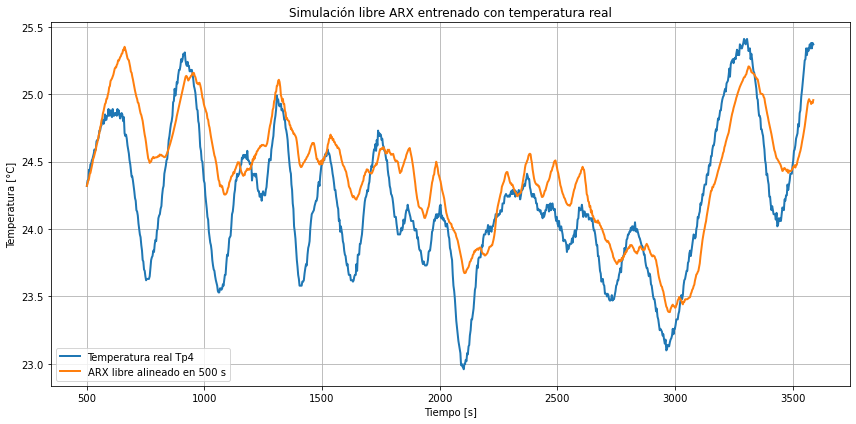
\includegraphics[width=0.75\linewidth]{SIMULACIONLIBREARX2conTrealdebase.png}
    \caption{Simulación del segundo modelo ARX.}
    \label{fig:Simulacionlibre}
\end{figure}
Se obtienen los siguientes indicadores temporales para esta simulación:
\begin{itemize}
    \item RMSE: 0.383887 °C
    \item MAE: 0.309448 °C
    \item FIT: 26.878 \%
    \item R²: 0.465315
\end{itemize}
Si bien el desempeño es inferior al obtenido en validaciones utilizando salidas reales del sistema, este comportamiento es esperable debido a que esta simulación constituye una prueba más exigente. El RMSE y MAE indican que la diferencia promedio entre la temperatura real y la estimada por el modelo es inferior a 1°C, lo que representa un  error relativamente bajo, considerando la naturaleza dinámica y lenta del sistema térmico. Por otra parte, el valor del FIT cercano a 27\% y el coeficiente $R^2$ de 0.46 muestran que, si bien el modelo logra reproducir parte importante de la dinámica del sistema, aún existen diferencias relevantes entre la respuesta real y la simulada.
\end{comment}
\subsubsection{Simulación libre}

Una vez seleccionada la estructura ARX dentro de la malla exploratoria, se procedió a evaluar su comportamiento mediante simulación libre. Esta etapa resulta especialmente importante en este primer modelo, ya que permite determinar si el buen desempeño relativo utilizado para seleccionar sus órdenes se mantiene cuando el modelo debe generar autónomamente la evolución de la temperatura.


En simulación libre, el modelo obtuvo un RMSE = 8.6566 °C, MAE = 8.6491 °C, $R^2$=−267.6743 y FIT = -1539.13 \%. Estos valores evidencian que la estructura seleccionada no proporciona una representación adecuada de la temperatura absoluta. En particular, los valores fuertemente negativos de $R^2$ y FIT muestran que el error de simulación es considerable respecto de la variabilidad presente en la señal medida. Por lo tanto, aunque esta estructura corresponde al mejor candidato dentro de la exploración realizada, sus resultados no permiten considerarla un modelo validado del sistema.


En la Figura \ref{fig:SimLibrelibrelibre} se compara la temperatura medida con la respuesta obtenida por el modelo ARX en simulación libre. Se observa una desviación sostenida de aproximadamente 8 a 10 °C entre ambas señales, lo que evidencia que el modelo no reproduce adecuadamente el nivel absoluto de la temperatura. Aunque la respuesta simulada conserva algunas variaciones temporales similares a las presentes en los datos experimentales, estas coincidencias no son suficientes para representar de forma satisfactoria la dinámica global del sistema. El desplazamiento persistente entre ambas curvas confirma que la estructura identificada presenta una capacidad limitada para reproducir la evolución térmica del proceso en simulación libre.


\begin{figure}[H]
    \centering
    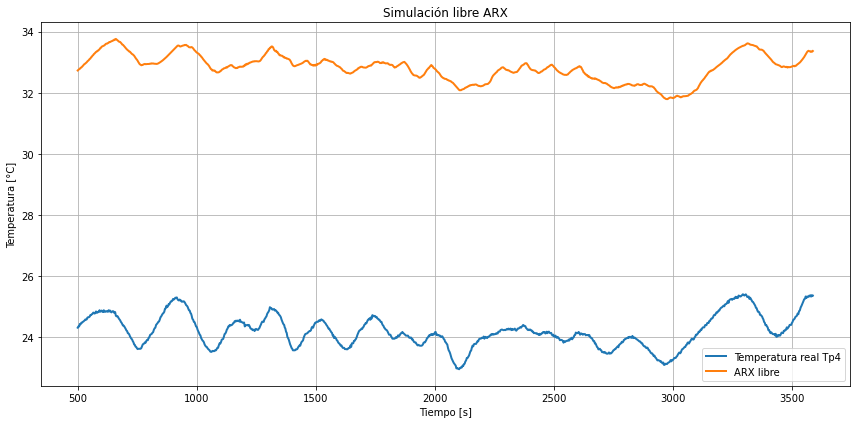
\includegraphics[width=0.65\linewidth]{SIMULACION LIBRELIBRELIBRE.png}
    \caption{Simulación libre del modelo ARX.}
    \label{fig:SimLibrelibrelibre}
\end{figure}

\begin{comment}
    

El análisis de los residuos (Figura \ref{fig:residosARX2libre}) refuerza esta conclusión. En lugar de presentar un comportamiento aleatorio alrededor de cero, los residuos muestran una forma estructurada, con una tendencia oscilatoria claramente definida. Esto indica que el error no corresponde únicamente a ruido de medición, sino que contiene información dinámica que el modelo no fue capaz de reproducir. Además, la magnitud de los residuos, superior a 8 °C en promedio, confirma que la discrepancia entre la salida simulada y la salida real es significativa.
\begin{figure}[H]
    \centering
    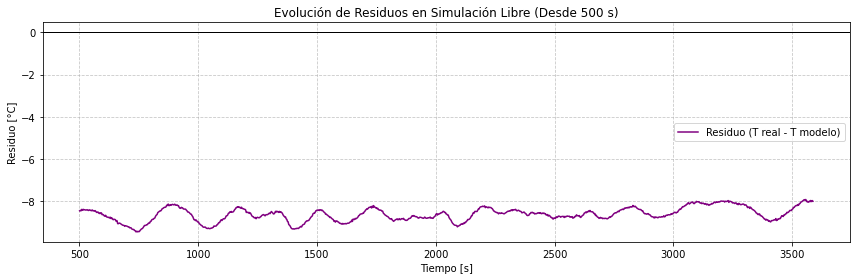
\includegraphics[width=0.5\linewidth]{RESIDUOSlibresLibres.png}
    \caption{Residuos del modelo en simulación libre.}
    \label{fig:residosARX2libre}
\end{figure}


La correlación cruzada entre la entrada y los residuos, mostrada en la Figura \ref{fig:correlacionE-R}, evidencia la presencia de correlaciones significativas. Este resultado es relevante, ya que un modelo adecuado debería generar residuos no correlacionados con la entrada. Si los residuos mantienen una relación dinámica con la señal de excitación, significa que parte del efecto de la entrada sobre la salida no fue capturado por la estructura del modelo \cite{ljung1999system}. En consecuencia, el modelo no logra representar completamente la dinámica térmica del sistema, quedando información útil aún contenida en el error de simulación.
\begin{figure}[H]
    \centering
    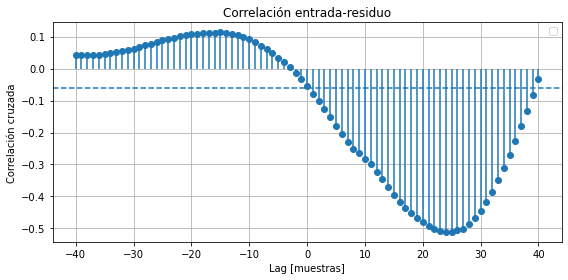
\includegraphics[width=0.5\linewidth]{correlacion entrada residuo arx2SiMULACIONLIBRE.png}
    \caption{Correlación entre la entrada y los residuos del modelo en simulación libre.}
    \label{fig:correlacionE-R}
\end{figure}

Desde el punto de vista frecuencial, la densidad espectral de la salida simulada y de la salida real presenta una tendencia similar en bajas frecuencias, donde se concentra la dinámica dominante del sistema térmico. Esto indica que el modelo reproduce parcialmente el contenido energético principal de la señal y las variaciones lentas asociadas al comportamiento del proceso. No obstante, la PSD del modelo presenta menores magnitudes que la señal real en parte de la banda de interés. Esta diferencia sugiere que el modelo atenúa ciertas componentes dinámicas presentes en la respuesta real, generando una salida más suavizada y con menor energía espectral. Por lo tanto, aunque la estructura ARX captura parte de la tendencia frecuencial general, no logra representar completamente la amplitud de las variaciones observadas en la temperatura medida.

\begin{figure}[H]
    \centering
    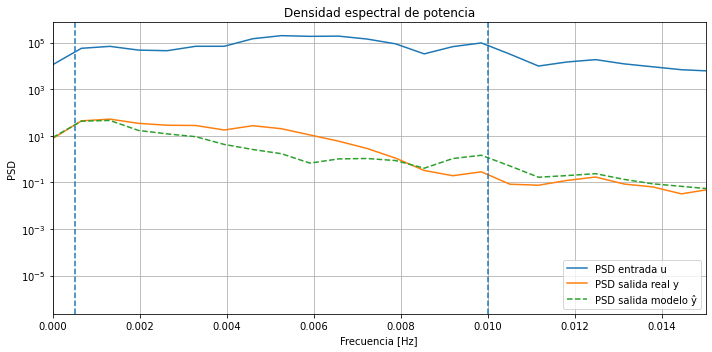
\includegraphics[width=0.5\linewidth]{DENSIDADarx2Simulacionlibre.png}
    \caption{Densidad espectral en simulación libre.}
    \label{fig:PSDarx2SimulacionLibre}
\end{figure}


El análisis de la función de respuesta en frecuencia, presentado en la Figura \ref{fig:comparacion_frfsimulacionlibre}, permite complementar esta evaluación. En magnitud, el modelo sigue la tendencia general de la FRF dentro de la banda de interés, especialmente entre 0.0005 Hz y 0.01 Hz. Sin embargo, se observan diferencias importantes en amplitud, particularmente en la zona media del espectro, donde el modelo tiende a subestimar la respuesta del sistema. En fase, la forma global de la curva simulada es similar a la real, lo que sugiere que el modelo representa parcialmente el retardo y el comportamiento dinámico dominante. Aun así, las diferencias observadas indican que existen componentes dinámicas secundarias que no son capturadas adecuadamente.

\begin{figure}[H]
    \centering
    \begin{subfigure}{0.6\linewidth}
    \centering
    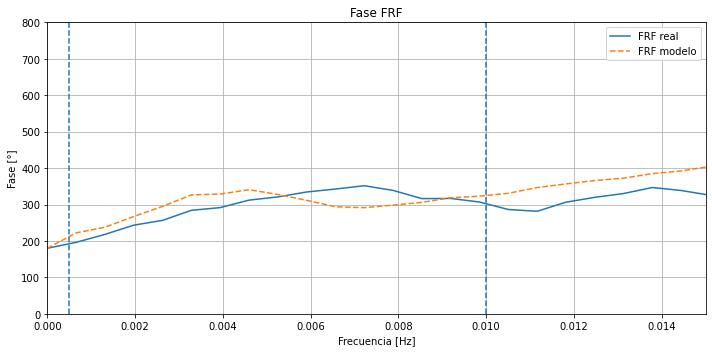
\includegraphics[width=0.6\linewidth]{FRFFsimulacionLibreARX2.png}
    \caption{Fase FRF en simulación libre.}
    \label{fig:FRFmagnitudSimLi}
    \end{subfigure}
    \hfill 
    \begin{subfigure}{0.6\linewidth}
      \centering
    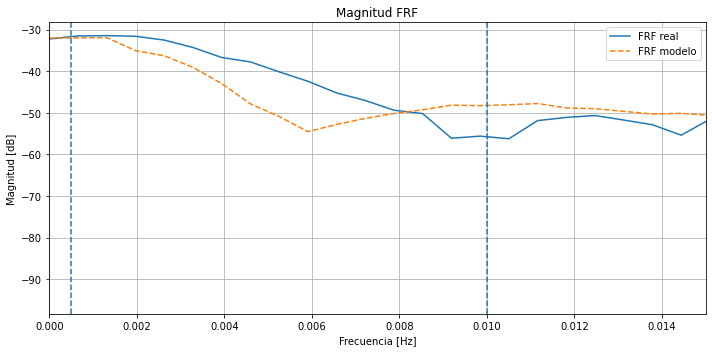
\includegraphics[width=0.6\linewidth]{FRFMsimulacionLibreARX2.png}
    \caption{Magnitud FRF en simulación libre.}
    \label{fig:FRFfaseSimLi}
    \end{subfigure}
    \caption{Respuesta en frecuencia del modelo es simulación libre.}
    \label{fig:comparacion_frfsimulacionlibre}
\end{figure}
\end{comment}

Los resultados muestran que esta primera estructura ARX debe considerarse un modelo exploratorio y no una representación final del sistema. Aunque la respuesta simulada conserva algunas variaciones temporales semejantes a las observadas en la temperatura real, el desempeño global en simulación libre es insuficiente. La existencia de un error sostenido de magnitud considerable, los valores negativos de $R^2$ y FIT evidencian que permanece una parte importante de la dinámica sin representar adecuadamente.

Estos resultados cumplen, sin embargo, un propósito relevante dentro del proceso de identificación, ya que permiten identificar las limitaciones de la primera formulación utilizada. En particular, muestran que la selección de órdenes dentro de la malla explorada, aun cuando permite obtener el mejor candidato según los criterios de búsqueda establecidos, no garantiza por sí sola una adecuada capacidad de simulación. Por lo tanto, resulta necesario revisar la formulación del problema y continuar con nuevas estrategias de identificación orientadas a reducir el error acumulado, mejorar el comportamiento de los residuos y obtener una representación más consistente de la dinámica térmica.

En consecuencia, esta primera etapa se utiliza como referencia para las modificaciones posteriores del proceso de modelación, manteniendo la estructura ARX como objeto de estudio, pero reconsiderando la forma en que se representa y procesa la variable de salida antes de avanzar hacia una nueva identificación.

\subsection{Segundo modelo ARX}

Los resultados obtenidos con el primer modelo ARX mostraron que la identificación realizada directamente sobre la temperatura absoluta no permitía reproducir adecuadamente la respuesta del sistema en simulación libre. En particular, se observó un desplazamiento sostenido entre la temperatura medida y la simulada, acompañado de errores temporales elevados. A partir de estos resultados, se planteó una segunda estrategia de identificación manteniendo la estructura ARX, pero modificando la forma en que se representa la variable de salida.

En esta segunda etapa, la identificación se realizó utilizando la variación de temperatura respecto de una condición térmica de referencia, en lugar de emplear directamente la temperatura absoluta. Para ello, se consideró como referencia la temperatura medida una vez transcurridos los primeros 500 segundos del ensayo. Este intervalo corresponde al período inicial de estabilización del banco de ensayos, durante el cual la temperatura evoluciona desde su condición inicial hasta alcanzar un nivel térmico más estable. A partir de este instante se definió la variable de salida como:

$$\Delta y(k)=y(k)-y_0$$
donde $y(k)$ corresponde a la temperatura medida para cada instante posterior al período de estabilización, mientras que $y_0$ representa la temperatura de referencia del sistema en la condición de estabilización (en los 500 segundos).


Esta transformación permite que el modelo describa la dinámica de la temperatura en términos de variaciones respecto al punto de operación, en lugar de intentar reproducir directamente el nivel absoluto de la señal. La respuesta dinámica relevante del sistema no está necesariamente asociada al valor absoluto de la temperatura, sino a cómo esta cambia frente a variaciones en la entrada. Al trabajar con $\Delta y(k)$ se reduce la influencia del nivel térmico inicial y se concentra la identificación en la evolución dinámica provocada por la señal de excitación.

Además, esta formulación es coherente con el comportamiento del banco de ensayos, ya que antes de aplicar o analizar la excitación principal existe un periodo de estabilización. Durante este intervalo, el sistema alcanza una condición inicial representativa, desde la cual las variaciones posteriores de temperatura pueden atribuirse principalmente al efecto dinámico de la entrada. Por lo tanto, modelar la salida como una diferencia respecto a dicha condición permite obtener una representación más centrada en la dinámica del proceso y menos dependiente del nivel térmico inicial.
El uso de $\Delta y$ no elimina la dinámica física del sistema, sino que modifica la referencia respecto de la cual esta se representa. Por lo tanto, las variaciones, retardos y efectos asociados a la inercia térmica permanecen contenidos en los datos, pero son expresados respecto de una condición térmica de referencia. Posteriormente, la temperatura absoluta puede reconstruirse incorporando nuevamente el valor $y_0$.

Una vez definida la nueva variable de salida, se aplicó nuevamente el procedimiento de identificación y selección de estructuras ARX descrito anteriormente. En consecuencia, los órdenes del modelo no fueron fijados directamente a partir de los resultados del primer ARX, sino que se evaluaron nuevamente distintas combinaciones de $n_a$, $n_b$ y $n_k$, utilizando ahora $\Delta y$ como variable de salida. Para cada estructura candidata se estimaron sus parámetros y se evaluó su desempeño de acuerdo con los criterios establecidos para la selección del modelo.

Como resultado del proceso de búsqueda, la estructura seleccionada correspondió nuevamente a:
\begin{itemize}
    \item $n_{a}=17$
    \item $n_{b}=21$
    \item $n_{k}=9$ 
\end{itemize}


Los valores obtenidos corresponde al resultado de una nueva exploración realizada sobre los datos transformados. Esto indica que, dentro del conjunto de estructuras evaluadas, esta combinación presenta el mejor compromiso según los criterios definidos, aun cuando la variable de salida utilizada para la identificación fue modificada.


El parámetro $n_a$ mantiene la cantidad de salidas pasadas utilizadas para representar la memoria térmica del sistema, mientras que $n_b$ conserva el número de términos asociados a la entrada. Por su parte,$n_k=9$ representa un retardo equivalente a 18 segundos. Se mantienen los órdenes permitiendo comparar directamente el efecto de identificar el modelo sobre temperatura absoluta frente a identificarlo sobre variaciones de temperatura.

Como resultado, se obtuvo un nuevo conjunto de coeficientes para los polinomios autorregresivo y de entrada. Si bien el orden del modelo se mantiene, los parámetros estimados presentan variaciones respecto al modelo anterior, debido a que la identificación se realiza ahora sobre una salida centrada en el punto de operación. Esto permite que el modelo ajuste principalmente las variaciones dinámicas de la temperatura y no el nivel absoluto de la señal.

Los coeficientes obtenidos para el término autorregresivo del modelo fueron:

$$a = [   -5.41775190e-01; -1.11561327e+00;  4.45728368e-01;
     1.12343893e-01;  1.32428419e-01; $$   
     $$-1.27810372e-02; -5.58462303e-02; 1.99872139e-02;  1.86373223e-02;$$
     $$1.71059782e-02; -9.59973098e-02; 1.21813451e-03; 
     8.62633510e-02; $$
     $$2.11749198e-02; 1.08380635e-03;
     3.05198777e-02; -5.49950630e-02]$$
Mientras que los coeficientes asociados a la entrada fueron:
$$b = [-3.20375855e-02;-1.25167253e-02;  5.32512606e-04;
     1.89286370e-02; 2.33405749e-02;$$
     $$-1.22764914e-03;
    -3.93981480e-03;-4.37899201e-03; 2.15424430e-03;$$
    $$-2.62631805e-03; -2.19598510e-03;1.41711664e-03;
     6.25856021e-03;$$
     $$-5.16351615e-04; 5.74545667e-06;
    -5.47845752e-03; 6.29762900e-03; $$ 
    $$-1.97422499e-03;
     3.75882066e-03;  3.81334239e-03;-1.89367899e-02]
$$

La principal diferencia respecto del primer modelo ARX radica, por tanto, no en la cantidad de términos utilizados, sino en la definición de la variable que se busca representar. Mientras el primer modelo intentaba reproducir directamente el nivel absoluto de temperatura, esta segunda formulación concentra la identificación en las variaciones térmicas desarrolladas a partir de una condición de referencia. 

\begin{comment}
    
La identificación del modelo arrojó el gráfico de la Figura \ref{fig:ModeloARX3}, de la cual se observa que este puede seguir la forma global del sistema, con algunas subestimaciones al comienzo y sobrestimaciones hacia el final del experimento.
%Los indicadores temporales obtenidos aquí son: RMSE = 0.7424 °C y R² = 0.8309

\begin{figure}[H]
    \centering
    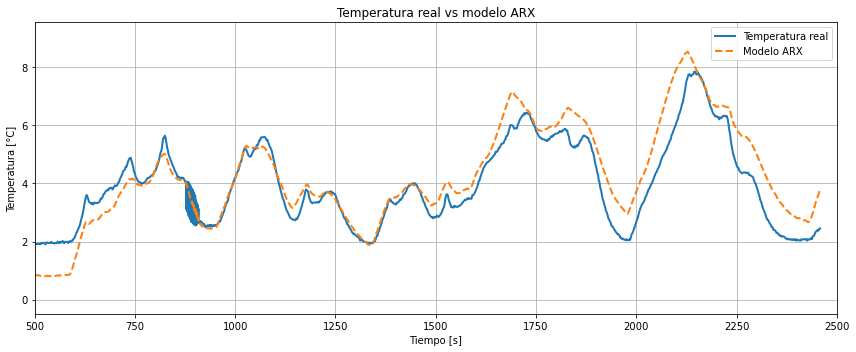
\includegraphics[width=0.5\linewidth]{ModeloARX3.png}
    \caption{Tercer modelo ARX.}
    \label{fig:ModeloARX3}
\end{figure}

\end{comment}
\begin{comment}
    

\subsubsection{Validación}
Al ser identificado con una variación de temperatura, la validación también se realizó con una variación de la salida real, la cual fue reconstruida mediante una temperatura de referencia, donde se utilizó la temperatura real a los 500 segundos, para poder tener una comparación visual y calcular métricas como RMSE, MAE y $R^2$.

Los resultados obtenidos mediante esta validación muestran un buen desempeño en la representación dinámica del sistema, Figura \ref{fig:validacionARX3}, dentro del rango de operación analizado.

\begin{figure}[H]
    \centering
    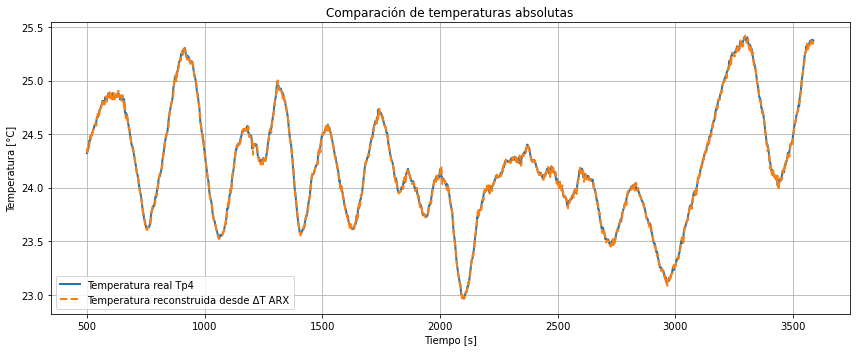
\includegraphics[width=0.5\linewidth]{ValidacionDeltaT.png}
    \caption{Temperatura entregada por el modelo vs temperatura real.}
    \label{fig:validacionARX3}
\end{figure}

Los indicadores temporales obtenidos corresponden a:
\begin{itemize}
    \item RMSE=0.0255°C
    \item MAE=0.0202°C
    \item $R^2$=0.9977
    \item FIT=95.16\%
\end{itemize}
El bajo valor de RMSE y MAE indica que las diferencias entre la señal real y la señal estimada por el modelo son muy pequeñas, con errores promedio del orden de centésimas de grados Celsius. Asimismo, el valor de $R^2$ demuestra que el modelo es capaz de explicar más del 99\% de la variabilidad de señal $\Delta T$, mientras que el FIT superior a 95\% evidencia un ajuste temporal bueno entre la respuesta real y la estimada.

El análisis de residuos (Figura \ref{fig:ErrorARX3}) muestran que estos permanecen centrados alrededor de cero y distribuido de manera aproximadamente aleatorio, lo que sugiere que el modelo captura adecuadamente la mayor parte de la dinámica presente en los datos experimentales.
La correlación cruzada entre la entrada y los residuos, Figura \ref{fig:CorrelacionARX3}, indica que los residuos son prácticamente independientes de la señal de entrada, con valores muy pequeños no observables en el gráfico. Esto es un resultado favorable, ya que evidencia que el modelo capturó la mayoría de la dinámica disponible.
El en dominio frecuencial, la PSD de la salida real y la salida estimada, observada en la Figura \ref{fig:PSDARX3}, presentan una coincidencia total en todo el rango de frecuencias analizado, indicando que el modelo reproduce adecuadamente la distribución de energía y el contenido espectral de la dinámica térmica del sistema.
De igual manera, la FRF de magnitud y fase del modelo (Figuras \ref{fig:FRFARXM} y \ref{fig:FRFARXF}) coinciden casi completamente con todas las obtenidas experimentalmente, evidenciando que el modelo representa correctamente tanto la ganancia dinámica como el comportamiento en fase del sistema dentro de la banda de frecuencia de interés. 

\begin{figure}[H]
    \centering

    % --- Fila 1: Residuos ---
    \begin{subfigure}[b]{0.48\textwidth}
        \centering
        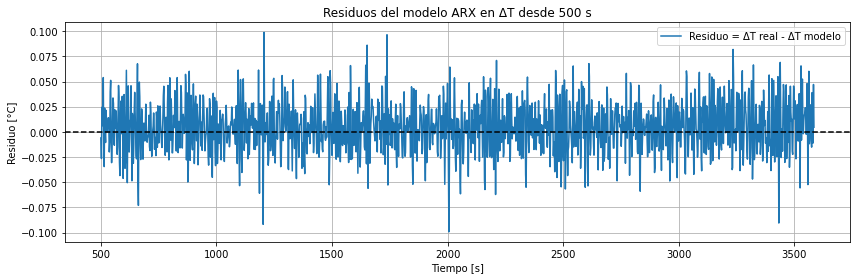
\includegraphics[width=\linewidth]{Figure 2026-05-20 150008 (1).png}
        \caption{Residuos del tercer modelo ARX.}
        \label{fig:ErrorARX3}
    \end{subfigure}
    \hfill % Espacio horizontal entre subfiguras
    \begin{subfigure}[b]{0.48\textwidth}
        \centering
        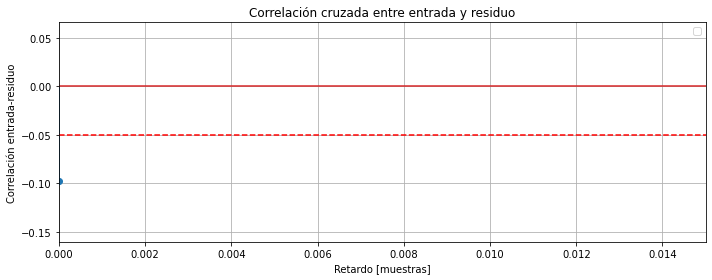
\includegraphics[width=\linewidth]{correlacionentradaresiduo.png}
        \caption{Correlación entrada y residuos.}
        \label{fig:CorrelacionARX3}
    \end{subfigure}

    \vspace{1em} % Espacio vertical entre filas

    % --- Fila 2: PSD y Magnitud FRF ---
    \begin{subfigure}[b]{0.48\textwidth}
        \centering
        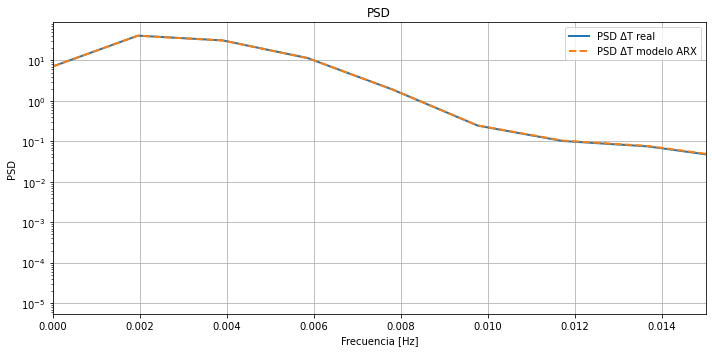
\includegraphics[width=\linewidth]{Figure 2026-05-20 150008 (5).png}
        \caption{Comparación de PSD real y modelo.}
        \label{fig:PSDARX3}
    \end{subfigure}
    \hfill
    \begin{subfigure}[b]{0.48\textwidth}
        \centering
        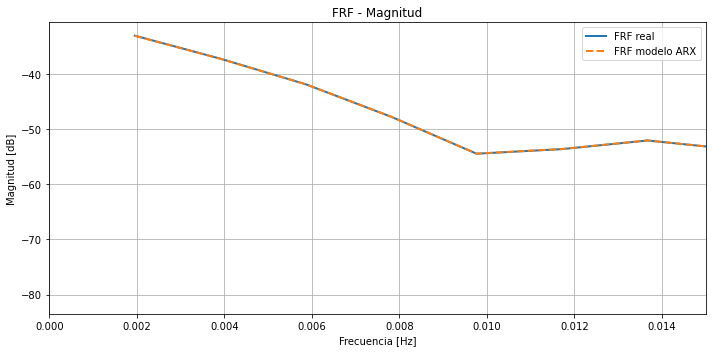
\includegraphics[width=\linewidth]{Figure 2026-05-20 150008 (7).png}
        \caption{Magnitud de FRF.}
        \label{fig:FRFARXM}
    \end{subfigure}

    \vspace{1em} % Espacio vertical entre filas

    % --- Fila 3: Fase FRF (centrada) ---
    \begin{subfigure}[b]{0.48\textwidth}
        \centering
        % La última imagen se mantendrá a la izquierda si no se hace nada.
        % Al usar un ancho total de 1 y centrar la figura, 
        % esta imagen se centrará en la fila.
        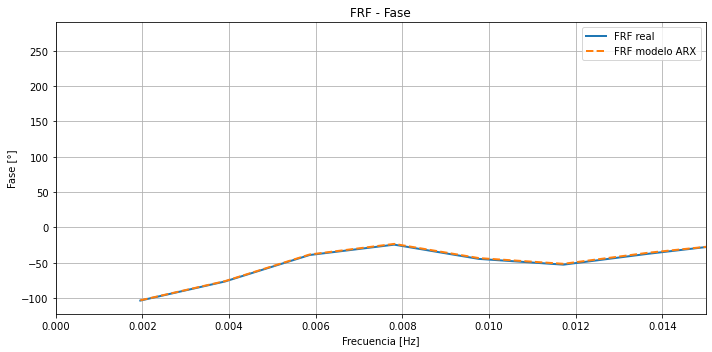
\includegraphics[width=\linewidth]{Figure 2026-05-20 150008 (8).png}
        \caption{Fase de FRF.}
        \label{fig:FRFARXF}
    \end{subfigure}
    % Se deja vacío el espacio de la derecha para centrar la última imagen

    % --- Título General ---
    \caption{Resultados del análisis y validación del tercer modelo ARX. Se muestran los residuos (a), su correlación con la entrada (b), la comparación de la Densidad Espectral de Potencia (PSD) (c), y la magnitud (d) y fase (e) de la Función de Respuesta en Frecuencia (FRF).}
    \label{fig:ResultadosCompletosARX3}

\end{figure}
En conjunto, los resultados obtenidos permiten concluir que el modelo ARX identificado sobre $\Delta T$ representa de forma precisa la dinámica incremental del sistema térmico alrededor del punto de operación considerado, constituyendo una representación adecuada para el sistema. Sin embargo, esto debe ser corroborado mediante un análisis de simulación libre, con lo cual se aseguraría la capacidad del modelo.
\end{comment}
\begin{comment}
    

\subsubsection{Primera simulación}

Se realizó una primera simulación, de igual manera que con el segundo modelo ARX, entregando la temperatura real a los 500 segundos y ajustando la curva. La Figura \ref{fig:SimulacionLibreARX3} muestra el comportamiento de este tercer modelo al entregarle el caudal de entrada al sistema, el cual sigue casi completamente la forma del gráfico, con algunas variaciones. Se observa también que en el vecindario cercano a los 1500 segundos, la dos curvas se sobreponen, siendo la estimación del modelo igual a la temperatura real.
\begin{figure}[H]
    \centering
    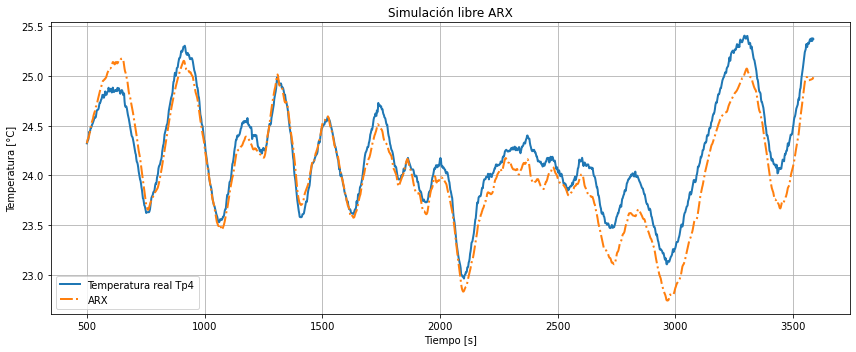
\includegraphics[width=0.65\linewidth]{Figure 2026-05-20 183404.png}
    \caption{Tercer modelo ARX con ajuste.}
    \label{fig:SimulacionLibreARX3}
\end{figure}
Los indicadores temporales fueron calculados con temperaturas absolutas para poder hacer la comparación con los otros modelos. 
\begin{itemize}
    \item RMSE = 0.2293 °C
    \item MAE  = 0.1898 °C
    \item R²   = 0.8102
    \item FIT  = 56.44 %
\end{itemize}
Al comparar este tercer modelo con el anterior, se entiende que los indicadores temporales dan una mejor simulación en este, obteniendo menores errores, una mayor explicación de la variabilidad de la señal $\Delta T$, 81\%, y un mejor ajuste temporal entre la respuesta real y la estimada con un FIT mayor a 56\%. 

\end{comment}
\subsubsection{Simulación libre}
La simulación libre del segundo modelo ARX se realizó considerando que la salida identificada corresponde a una variación de temperatura, es decir, a una señal expresada como $\Delta T$ . Por esta razón, para comparar la respuesta estimada con la temperatura real del sistema, la salida entregada por el modelo fue reconstruida en escala absoluta sumando una temperatura base, donde se utilizó como referencia la temperatura ambiente registrada al momento de realizar la adquisición de datos reales. 


De esta manera, el modelo fue evaluado sin entregar información de la salida real durante la simulación. Es decir, la respuesta se generó de forma recursiva utilizando únicamente la entrada aplicada y las salidas previamente estimadas por el propio modelo. El resultado se presenta en la Figura \ref{fig:SimLibrelibreARX3}. Al comparar esta respuesta con la obtenida por el modelo ARX anterior, mostrada en la Figura \ref{fig:SimLibrelibrelibre}, se observa una mejora importante en la aproximación a la temperatura real. En particular, el segundo modelo conserva de mejor manera la forma global de la curva y reduce considerablemente el error medio de simulación.




\begin{figure}[H]
    \centering
    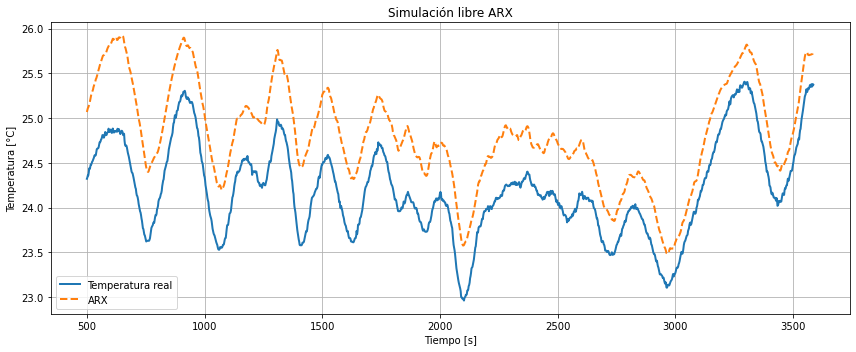
\includegraphics[width=0.5\linewidth]{SIMULACIONlibrelibrelibre.png}
    \caption{Comportamiento en simulación libre del segundo modelo ARX.}
    \label{fig:SimLibrelibreARX3}
\end{figure}


Los indicadores temporales obtenidos para este modelo fueron:
\begin{itemize}
    \item RMSE                 = 0.623598 °C
\item MAE                  = 0.598302 °C
\item $R^2$                   = -0.403776
\item FIT                  = -18.481 \%

\end{itemize}

Aunque los valores de $R^2$ y FIT siguen indicando un desempeño global limitado, los errores RMSE y MAE muestran una mejora significativa respecto al modelo ARX anterior, ya que el error promedio se mantiene por debajo de 1 °C. Esto indica que el uso de la variable $\Delta T$ permitió mejorar la representación de la respuesta térmica en simulación libre, especialmente en términos de magnitud del error.



La gráfica de residuos, presentada en la Figura \ref{fig:residuosARX3simli}, muestra que estos se mantienen aproximadamente entre 0 y -1 °C. Sin embargo, la curva de error no presenta un comportamiento completamente aleatorio, sino que conserva una estructura definida. Esto indica que, aunque el error disminuye en magnitud, todavía existen componentes dinámicas no representadas adecuadamente por el modelo. En particular, la presencia de una tendencia o sesgo en los residuos sugiere que la estructura ARX no logra capturar por completo toda la variabilidad de la temperatura.
La correlación cruzada (Figura \ref{fig:correlacionARXsimli}) muestra correlación significativa, indicando que  parte de la información de la entrada permanece en el residuo, por lo que el modelo no logró capturar completamente toda la dinámica inducida por el caudal. Sin embargo, la PSD \ref{fig:PSDARX3simli} de la simulación y de los datos reales prácticamente coincide en la banda de interés, con lo cual el contenido energético principal del sistema está correctamente modelado.
A pesar de lo anterior, el análisis frecuencial muestra un comportamiento favorable. La densidad espectral de la salida simulada y de la salida real (Figura \ref{fig:PSDARX3simli}) presenta una alta coincidencia dentro de la banda de interés. Esto indica que el modelo reproduce adecuadamente el contenido energético dominante de la respuesta térmica, especialmente en bajas frecuencias, donde se concentra la dinámica principal del sistema. Por lo tanto, aunque el modelo mantiene errores en el dominio temporal, su representación frecuencial resulta coherente con el comportamiento observado en los datos reales.

De manera complementaria, la función de respuesta en frecuencia muestra una tendencia similar entre el modelo y el sistema real, tanto en magnitud como en fase. La similitud en magnitud indica que el modelo reproduce razonablemente la forma en que las variaciones del caudal afectan la amplitud de la respuesta térmica en función de la frecuencia. Por otra parte, la similitud en fase sugiere que el modelo captura de forma aceptable el retardo y la evolución temporal dominante del sistema. Estos resultados refuerzan la idea de que el segundo modelo ARX logra representar la dinámica principal del proceso en la banda de bajas frecuencias.




\begin{figure}[H]
    \centering
    
    % Fila 1: Residuos y Correlación
    \begin{subfigure}[b]{0.48\linewidth}
        \centering
        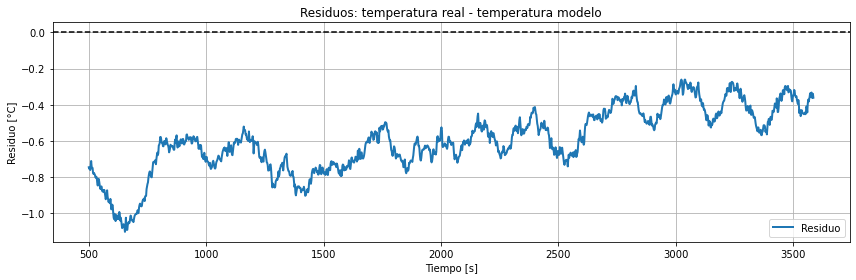
\includegraphics[width=\linewidth]{residuosLIBRESLIBRES.png}
        \caption{Residuos en simulación libre.}
        \label{fig:residuosARX3simli}
    \end{subfigure}
    \hfill
    \begin{subfigure}[b]{0.48\linewidth}
        \centering
        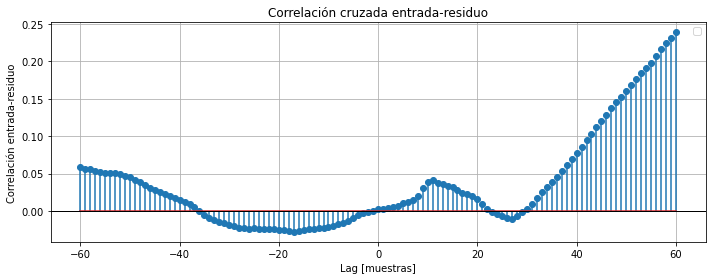
\includegraphics[width=\linewidth]{Figure 2026-05-20 215807 (7).png}
        \caption{Correlación entrada-residuos.}
        \label{fig:correlacionARXsimli}
    \end{subfigure}

    \vspace{0.3cm} % Espacio vertical entre filas

    % Fila 2: Densidad espectral y Magnitud de FRF
    \begin{subfigure}[b]{0.48\linewidth}
        \centering
        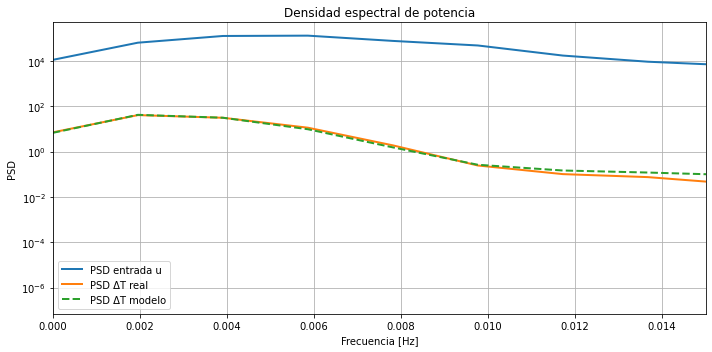
\includegraphics[width=\linewidth]{Figure 2026-05-20 215807 (8).png}
        \caption{Densidad espectral del modelo.}
        \label{fig:PSDARX3simli}
    \end{subfigure}
    \hfill
    \begin{subfigure}[b]{0.48\linewidth}
        \centering
        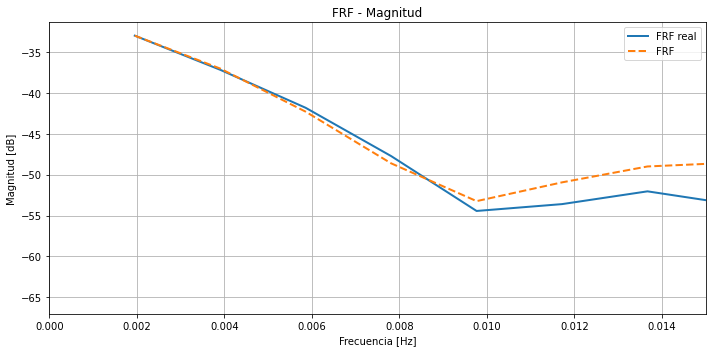
\includegraphics[width=\linewidth]{Figure 2026-05-20 215807 (10).png}
        \caption{Magnitud de FRF.}
        \label{fig:frfMarxsimli}
    \end{subfigure}

    \vspace{0.3cm}

    % Fila 3: Fase de FRF (Centrado abajo)
    \begin{subfigure}[b]{0.48\linewidth}
        \centering
        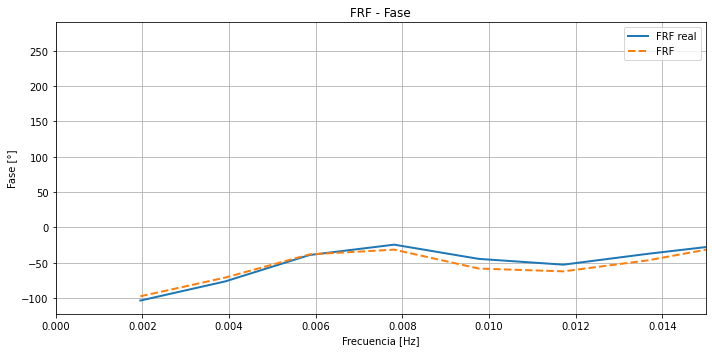
\includegraphics[width=\linewidth]{Figure 2026-05-20 215807 (11).png}
        \caption{Fase de FRF.}
        \label{fig:frfFsimli}
    \end{subfigure}

    \caption{Resultados del análisis y validación del segundo modelo ARX en simulación libre.}
    \label{fig:conjunto_arx_simli}
\end{figure}

En conjunto, el modelo identificado utilizando la salida en forma de $\Delta T$ presenta un mejor desempeño en simulación libre que el modelo ARX anterior. La reducción del error medio, junto con la similitud observada en la PSD y en la FRF, indica que esta formulación permite representar de mejor manera la dinámica dominante del sistema térmico. Sin embargo, los valores negativos de $R^2$ y FIT, junto con la estructura observada en los residuos y la correlación significativa entre entrada y error, evidencian que el modelo aún no captura completamente toda la dinámica del sistema.

Por esta razón, se justifica avanzar hacia una nueva estructura de modelado. En particular, resulta pertinente evaluar un modelo Output-Error (OE), ya que esta estructura separa de forma más explícita la dinámica del sistema del tratamiento del error. A diferencia del modelo ARX, donde la dinámica de la salida y la descripción del ruido quedan acopladas dentro de una misma estructura autorregresiva, el modelo OE busca representar directamente la relación dinámica entre la entrada y la salida. Esto puede resultar más adecuado para mejorar la simulación libre, ya que el objetivo principal es reproducir la respuesta del sistema frente a una entrada conocida. En consecuencia, la identificación de un modelo OE se plantea como una alternativa para mejorar la representación dinámica del banco de ensayos y reducir la presencia de información no modelada en los residuos.

\subsection{Modelo Output Error (OE)}

A partir de los resultados obtenidos con los modelos ARX, se consideró necesario evaluar una estructura alternativa que permitiera representar con mayor precisión la dinámica del sistema térmico. Si bien los modelos ARX constituyeron una primera aproximación útil y permitieron identificar parte del comportamiento dominante del proceso, su validación evidenció limitaciones asociadas a la presencia de residuos estructurados, correlación entre la entrada y el error.

En este contexto, se seleccionó una estructura Output-Error (OE) como siguiente etapa de modelación. A diferencia del modelo ARX, en el cual la salida se representa mediante una estructura autorregresiva que incorpora conjuntamente la dinámica del sistema y el efecto del error, el modelo OE describe de manera directa la relación determinística entre la entrada y la salida, mientras que el error de medición se considera externamente a dicha dinámica. Esta separación permite orientar la estimación hacia el comportamiento propio del proceso y resulta especialmente conveniente cuando el objetivo principal es obtener una adecuada respuesta en simulación.

La elección del modelo OE se relaciona directamente con las limitaciones observadas en el segundo modelo ARX. Aunque la utilización de la variación de temperatura permitió mejorar considerablemente su desempeño respecto del primer modelo exploratorio, los residuos aún presentaron estructura y conservaron correlación con la entrada. Esto indica que parte de la información dinámica asociada al caudal no fue representada completamente por la estructura ARX.

Por otra parte, en simulación libre la componente autorregresiva del modelo ARX obliga a utilizar de manera recursiva las propias salidas estimadas. En estas condiciones, pequeños errores pueden propagarse y acumularse a medida que avanza la simulación, efecto que adquiere especial relevancia en un sistema térmico caracterizado por una dinámica lenta y una respuesta prolongada en el tiempo. El modelo OE evita incorporar salidas pasadas como parte de la dinámica determinística y representa la respuesta mediante la acción filtrada de la entrada, por lo que constituye una alternativa adecuada para evaluar si una formulación distinta permite mejorar la reproducción de la evolución térmica del sistema.

En consecuencia, el paso desde ARX hacia OE no implica descartar el enfoque lineal, sino modificar la estructura utilizada para representar la relación entrada–salida. De esta manera, es posible determinar si las limitaciones observadas se deben principalmente a la formulación autorregresiva del modelo o si persisten aun cuando la dinámica del proceso se representa mediante una estructura lineal diferente.

\subsection{Proceso de identificación y selección para el modelo Output-Error}


El proceso de identificación del modelo Output-Error (OE) se desarrolló mediante una exploración sistemática de distintas estructuras, siguiendo una estrategia similar a la utilizada para los modelos ARX. En este caso se mantuvo la representación de la salida mediante variaciones de temperatura, con el propósito de modelar la dinámica respecto de una condición de operación de referencia. A diferencia del ARX, la estimación del modelo OE requiere un procedimiento iterativo, debido a que su salida se obtiene recursivamente a partir de los parámetros del propio modelo. Por esta razón, la búsqueda de estructuras presenta un costo computacional mayor y requiere una estrategia específica de optimización.


\begin{enumerate}
    \item \textbf{Preparación y división de los datos}

    Se excluyeron los primeros 500 segundos del registro, correspondientes al período inicial de estabilización del sistema y posteriormente las señales fueron remuestreadas con un período uniforme de $T_s$=2 segundos. Para obtener una grilla temporal uniforme, se aplicó una interpolación lineal entre instantes de tiempo consecutivos. Esto se considera adecuado ya que la dinámica térmica del sistema se encuentra en el orden de los minutos en lugar del orden de los segundos. El conjunto resultante se dividió cronológicamente, utilizando el 80 \% inicial para la identificación y el 20 \% restante para la validación.

    \item \textbf{Preprocesamiento de las señales}

Al igual que en la identificación del modelo ARX, las señales utilizadas por el modelo OE fueron normalizadas antes de la estimación de los parámetros. Los factores de normalización se calcularon utilizando únicamente el conjunto de identificación y posteriormente se aplicaron tanto a los datos de identificación como a los de validación. Este procedimiento permite trabajar con variables en escalas comparables, mejorar el acondicionamiento numérico del problema y evitar que la información del conjunto de validación intervenga en la estimación del modelo.

    \item \textbf{Definición de las estructuras OE candidatas}




    Cada estructura OE fue definida mediante los órdenes $n_f$, $n_b$ y $n_k$. El parámetro $n_f$ determina el orden del polinomio denominador $F(q)$ y, por lo tanto, la cantidad de términos utilizados para reproducir la dinámica interna de la salida simulada. El parámetro $n_b$ determina el número de coeficientes del polinomio $B(q)$, correspondiente al numerador y encargado de representar la influencia de la entrada sobre la salida (Ecuación \ref{ecuacionOE}). Por su parte, $n_k$ representa el retardo discreto entre una variación del caudal y su efecto sobre la salida. A partir de estos tres parámetros se construyó una malla de estructuras candidatas, evaluando distintas combinaciones con el propósito de encontrar una representación adecuada de la dinámica del sistema sin incrementar innecesariamente la complejidad del modelo.

    \item \textbf{Estimación iterativa de los parámetros}

    Para cada combinación de órdenes se estimaron los coeficientes de los polinomios $F(q)$ y $B(q)$ mediante mínimos cuadrados no lineales. A diferencia del modelo ARX, en el OE la salida simulada depende recursivamente de valores previamente generados por el propio modelo. Como consecuencia, los parámetros no pueden obtenerse directamente mediante una única regresión lineal, sino que deben determinarse mediante un proceso iterativo que minimiza el error entre la salida medida y la simulada.

Para reducir la dependencia del resultado respecto del punto inicial de la optimización, cada estructura fue evaluada utilizando diferentes inicializaciones de los parámetros. Para cada una de ellas se ejecutó el algoritmo de optimización y se conservó la solución que presentó el menor costo.

    \item \textbf{Evaluación de las estructuras candidatas}


    
Una vez estimados los parámetros, cada modelo fue simulado utilizando tanto las entradas del conjunto de identificación como las del conjunto de validación. Su desempeño se cuantificó mediante RMSE y FIT. La evaluación sobre el conjunto de validación tuvo especial importancia, ya que permite determinar si la estructura conserva su capacidad de representación sobre datos que no participaron en la estimación de sus parámetros.

Adicionalmente, se analizaron los residuos de validación mediante un criterio asociado a su autocorrelación. La presencia de correlación temporal en los residuos indica que permanece información dinámica que el modelo no ha representado completamente, por lo que este comportamiento fue penalizado dentro del proceso de selección.

    
    \item \textbf{Evaluación de estabilidad y complejidad}

Para cada estructura se verificó la estabilidad mediante las raíces del polinomio F(q). Un modelo discreto se considera estable cuando todas las raíces se encuentran dentro del círculo unitario, las estructuras que no cumplían esta condición fueron fuertemente penalizadas. También se verificó que la ganancia en estado estacionario permaneciera dentro de valores razonables y se incorporó una penalización asociada al número de parámetros, con el propósito de evitar estructuras innecesariamente complejas.

\item \textbf{Selección preliminar del modelo}

Las estructuras fueron comparadas mediante una función de costo global que combinó el RMSE y FIT obtenidos en validación, el comportamiento de los residuos, la complejidad, la estabilidad y la ganancia del modelo. De esta forma, la selección no se realizó únicamente a partir del menor error, sino considerando conjuntamente diferentes propiedades necesarias para obtener una representación dinámica adecuada. Los modelos estables fueron ordenados según este criterio y se seleccionó la mejor combinación de $n_f$, $n_b$ y $n_k$.


\item \textbf{Optimización final}


Debido al mayor costo computacional asociado a la estimación OE, la búsqueda inicial permitió seleccionar la combinación de órdenes $n_f$, $n_b$ y $n_k$ más favorable entre las estructuras candidatas, pero una vez definida, los órdenes se mantuvieron fijos y se realizó una segunda etapa de optimización destinada exclusivamente a refinar los coeficientes de los polinomios $F(q)$ y $B(q)$. Para ello se utilizó el conjunto completo de datos de identificación, se aumentó el número de iteraciones permitidas y se probaron distintas condiciones iniciales cercanas a la solución obtenida en la búsqueda preliminar. Finalmente, se conservaron los coeficientes que produjeron el menor valor de la función de costo. De esta manera, la primera etapa selecciona la estructura del modelo, mientras que la segunda mejora la estimación de sus parámetros.


\item \textbf{Evaluación final y reconstrucción de la respuesta}

El modelo seleccionado fue finalmente evaluado sobre los conjuntos completos de identificación y validación mediante simulación, calculándose RMSE, FIT, MAE y $R^2$. Posteriormente, las transformaciones de normalización y centrado fueron revertidas para expresar nuevamente la respuesta en la escala física de temperatura y permitir su comparación directa con los datos experimentales.

\end{enumerate}


En conjunto, este procedimiento permitió seleccionar el modelo OE considerando no solo su capacidad para minimizar el error de simulación, sino también su estabilidad, complejidad y comportamiento residual. La utilización de una búsqueda preliminar seguida de una optimización final permitió además reducir el costo computacional asociado a la estimación iterativa característica de esta estructura.


A partir del procedimiento de identificación y selección descrito anteriormente, se obtuvo como mejor estructura candidata un modelo Output-Error definido por los órdenes:
\begin{itemize}
    \item $n_f=3$
    \item $n_b=9$
    \item $n_k=7$
\end{itemize}


Estos valores corresponden a la combinación que presentó el mejor desempeño dentro de la malla de estructuras evaluadas, considerando conjuntamente el error de validación, la estabilidad, la complejidad del modelo y el comportamiento de los residuos. Por lo tanto, los órdenes no fueron fijados previamente, sino determinados a partir del proceso de búsqueda y optimización aplicado a los datos.

El parámetro $n_f=3$ define el orden del polinomio $F(q)$, correspondiente al denominador del modelo OE. Este valor determina la complejidad de la dinámica interna utilizada para representar la evolución de la salida. Dentro de las estructuras evaluadas, un denominador de tercer orden proporcionó un equilibrio adecuado entre capacidad de representación y complejidad, evitando incorporar una cantidad innecesaria de parámetros.

Por su parte, $n_b=9$ establece el número de coeficientes del polinomio $B(q)$, encargado de representar la influencia de la entrada sobre la salida. En consecuencia, el modelo utiliza nueve términos asociados a valores retardados del caudal para describir su efecto sobre la variación de temperatura. Este orden fue seleccionado porque, dentro de la búsqueda realizada, permitió representar adecuadamente la contribución dinámica de la entrada sin aumentar excesivamente la complejidad de la estructura.

Finalmente, $n_k=7$ corresponde al retardo discreto entre la entrada y la salida. Considerando un período de muestreo de $T_s$=2 segundos, este valor equivale a aproximadamente 14 segundos. Esto significa que la estructura identificada considera que el efecto de una variación del caudal comienza a incorporarse en la respuesta modelada después de siete muestras. Al igual que los demás órdenes, este valor corresponde al resultado de la identificación y no a un retardo impuesto previamente a partir de consideraciones físicas.


Los polinomios obtenidos para el modelo identificado fueron:
$$B(q)=0.1734−0.5086q^{−1}+0.4715q^{−2}−0.1314q^{−3}+0.0175q^{−4}−0.0177q^{−5}−0.0283q^{−6}$$
$$+0.0387q^{−7}−0.0158q^{−8}$$
$$F(q)=1−2.8154q^{−1}+2.6431q^{−2}−0.8274q^{−3}$$

A partir de estos polinomios, el modelo OE puede interpretarse como una representación dinámica discreta de la relación entre el caudal de entrada y la variación de temperatura de salida. El polinomio $B(q)$ describe cómo las entradas retardadas contribuyen a la respuesta, mientras que $F(q)$ determina la forma de la dinámica del modelo, incluyendo la persistencia temporal de sus efectos y la evolución de la salida. De este modo, la estructura seleccionada permite representar la dinámica entrada-salida mediante un modelo de orden relativamente bajo, en comparación con el ARX previamente evaluado.


%$$y(k)=2.8154y(k−1)−2.6431y(k−2)+0.8274y(k−3)+0.1734u(k−7)−0.5086u(k−8)$$
%$$+0.4715u(k−9)−0.1314u(k−10)+0.0175u(k−11)−0.0177u(k−12)−0.0283u(k−13)$$
%$$+0.0387u(k−14)−0.0158u(k−15)$$
%La validación que entrega el mismo código de identificación del modelo es la Figura \ref{fig:modelooe}, donde se observa un buen seguimiento de este a la curva real de temperatura, después de los 500 segundos.
%\begin{figure}[H]
    %\centering
    %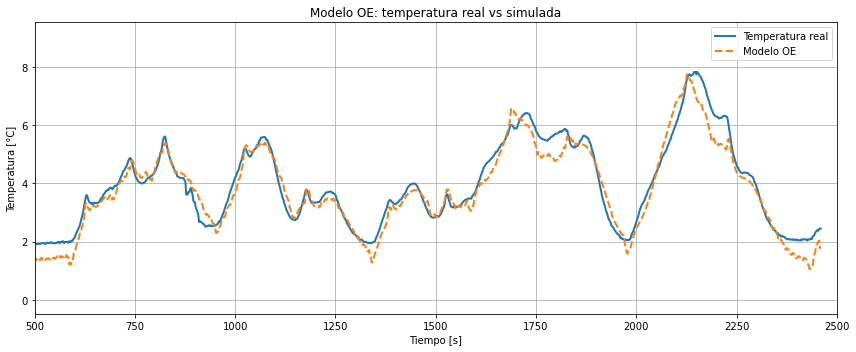
\includegraphics[width=0.65\linewidth]{ModeloOE.png}
    %\caption{Modelo OE}
    %\label{fig:modelooe}
%\end{figure}


\begin{comment}
    

\subsubsection{Primera simulación}
Debido a la estructura del modelo OE, la validación se hará netamente con simulación libre, ya que este por definición utiliza sus mismas salidas para reproducir el sistema.

La primera simulación fue realizada de la misma manera que con los modelos ARX anteriores, de lo cual se obtiene la siguiente curva, Figura \ref{fig:Simlioe}. Se observa que el modelo Output-Error sigue  la tendencia general y captura la mayoría de las oscilaciones, pero presenta diferencias en amplitud y desfases, subestimado o sobrestimando localmente, específicamente entre los 600 segundos y hacia el el final del experimento.
\begin{figure}[H]
    \centering
    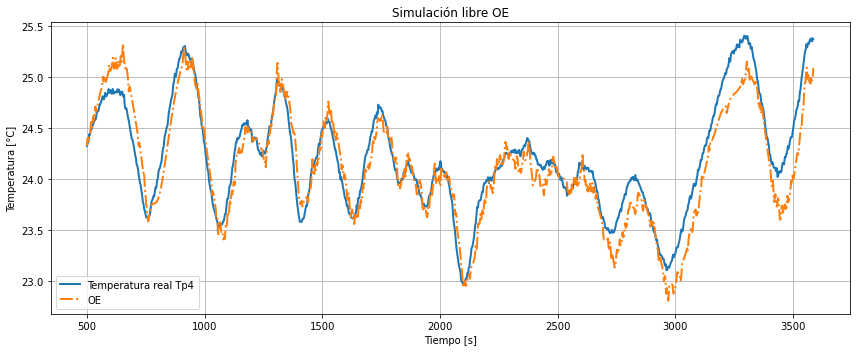
\includegraphics[width=0.5\linewidth]{Figure 2026-05-21 133410 (1).png}
    \caption{Primera validación del modelo Output-Error.}
    \label{fig:Simlioe}
\end{figure}


Los indicadores temporales que se obtuvieron son los siguientes:
\begin{itemize}
    \item RMSE = 0.2102 °C y MAE  = 0.1670 °C, el error es inferior al 0.25°C, siendo relativamente pequeño.
    \item FIT  = 60.07 \% , evidencia un ajuste temporal de más del 50\%, siendo la forma general de la respuesta capturada.
    \item R²   = 0.8406 indica que el modelo explica cerca del 84\% de la variabilidad de la señal real.
    
\end{itemize}
\end{comment}

\subsubsection{Simulación libre}
La simulación libre del modelo Output-Error se realizó bajo el mismo criterio utilizado para los modelos ARX, es decir, generando la respuesta del modelo a partir de la señal de entrada y de sus propias salidas estimadas, sin utilizar la salida real durante la simulación. El resultado se presenta en la Figura \ref{fig:SimLibreoe}.
\begin{figure}[H]
    \centering
    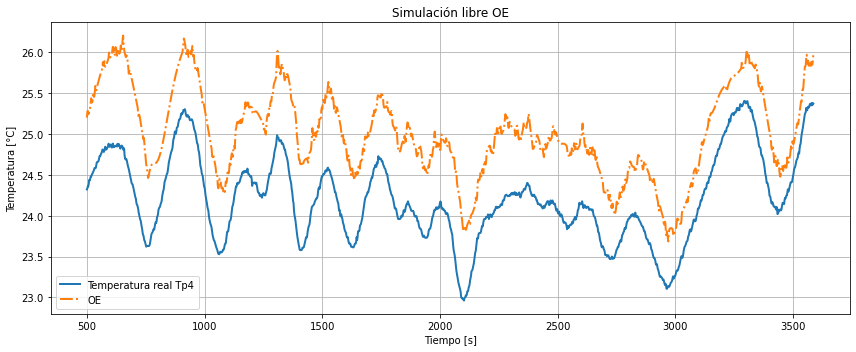
\includegraphics[width=0.65\linewidth]{SIMULACIONlibrelibre.png}
    \caption{Simulación libre del modelo Output-Error.}
    \label{fig:SimLibreoe}
\end{figure}

En términos generales, se observa que la respuesta simulada conserva una tendencia similar a la temperatura real del sistema. Sin embargo, persiste una diferencia sistemática entre ambas curvas, ya que el modelo tiende a sobrestimar la temperatura durante gran parte del ensayo. Esto indica que, aunque la estructura OE logra reproducir parcialmente la forma global de la respuesta térmica, aún presenta dificultades para ajustar correctamente el nivel de la señal en simulación libre.

Los indicadores temporales obtenidos son:
\begin{itemize}
    \item RMSE                 = 0.819204 °C
    \item MAE                  = 0.796064 °C
    \item $R^2 $                  = -1.422553
\item FIT                  = -55.646 \%
\end{itemize}

Los valores de RMSE y MAE indican que el error medio se mantiene bajo 1 °C, lo que representa un desempeño aceptable en términos de magnitud absoluta del error. Sin embargo, los valores negativos de $R^2$ y FIT evidencian que el modelo no logra explicar adecuadamente la variabilidad temporal de la temperatura real. Esto ocurre porque, aunque el error promedio no es elevado, existe un sesgo sistemático en la respuesta simulada, lo que afecta negativamente las métricas globales de ajuste.




El análisis de los residuos (Figura \ref{fig:residuosOE2simli}) confirma esta limitación. Los residuos no se distribuyen aleatoriamente alrededor de cero, sino que presentan oscilaciones claras y se mantienen mayoritariamente en valores negativos, aproximadamente entre -0.4 °C y -1.4 °C. Este comportamiento indica que el modelo sobrestima la temperatura y que el error conserva una estructura dinámica. 
La correlación cruzada entre la entrada y los residuos (Figura \ref{fig:correlacionOE2simli}) presenta valores significativos para distintos retardos. Esto indica que parte de la información asociada al caudal aún permanece en el error del modelo. Desde el punto de vista de la validación, este resultado es relevante, ya que un modelo adecuado debería generar residuos con baja correlación respecto de la entrada. La presencia de esta correlación sugiere que la estructura OE no ha capturado completamente la relación dinámica entre la entrada manipulada y la temperatura de salida.

Desde el punto de vista frecuencial, el modelo presenta un comportamiento más favorable. La densidad espectral de la salida simulada, observada en la Figura \ref{fig:PSDsimliOE2}, sigue de cerca la densidad espectral de la temperatura real en gran parte de la banda analizada. Esto indica que el modelo reproduce adecuadamente el contenido energético dominante de la respuesta térmica, especialmente en bajas frecuencias, donde se concentra la dinámica principal del sistema.

De manera complementaria, la función de respuesta en frecuencia muestra una concordancia aceptable entre el modelo y el sistema real. En la magnitud de la FRF (Figura \ref{fig:FRFmSimliOE2}) las curvas presentan valores similares dentro de la banda de interés, comenzando a separarse de forma más evidente cerca de 0.008 Hz. Esto sugiere que el modelo OE representa adecuadamente la dinámica lenta principal, pero pierde precisión al aumentar la frecuencia. En cuanto a la fase (Figura \ref{fig:FRFfsimliOE2}) ambas curvas presentan una tendencia general similar, aunque no coincidente. Esta diferencia puede estar asociada a un desajuste en el retardo efectivo del modelo o a una representación incompleta de la distribución dinámica del sistema.

\begin{figure}[H]
    \centering
    % Primera fila: Residuos y Correlación
    \begin{subfigure}[b]{0.48\textwidth}
        \centering
        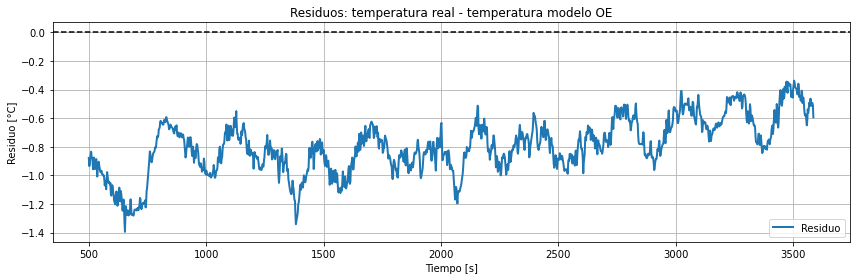
\includegraphics[width=\linewidth]{residuosSIMULACIONLIBRE.png}
        \caption{Residuos en la simulación libre del modelo OE.}
        \label{fig:residuosOE2simli}
    \end{subfigure}
    \hfill
    \begin{subfigure}[b]{0.48\textwidth}
        \centering
        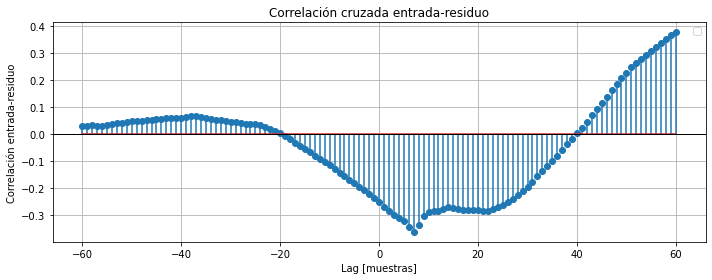
\includegraphics[width=\linewidth]{Figure 2026-05-21 133410 (7).png}
        \caption{Correlación entrada-residuos.}
        \label{fig:correlacionOE2simli}
    \end{subfigure}

    \vspace{0.3cm} % Espacio vertical entre filas

    % Segunda fila: Densidad espectral y Magnitud de FRF
    \begin{subfigure}[b]{0.48\textwidth}
        \centering
        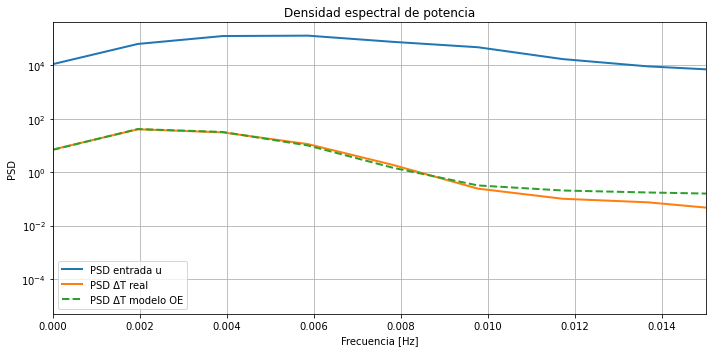
\includegraphics[width=\linewidth]{Figure 2026-05-21 133410 (8).png}
        \caption{Densidad espectral.}
        \label{fig:PSDsimliOE2}
    \end{subfigure}
    \hfill
    \begin{subfigure}[b]{0.48\textwidth}
        \centering
        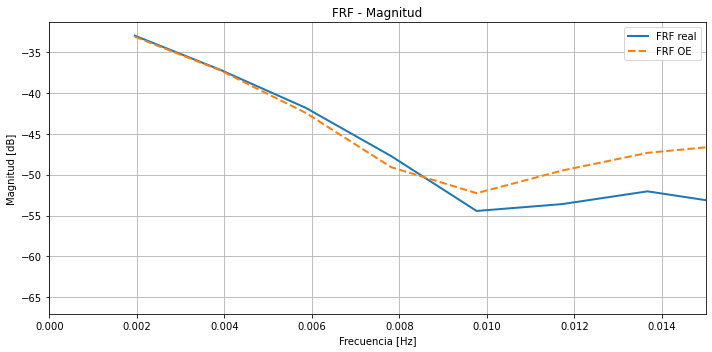
\includegraphics[width=\linewidth]{Figure 2026-05-21 133410 (10).png}
        \caption{Magnitud de FRF.}
        \label{fig:FRFmSimliOE2}
    \end{subfigure}

    \vspace{0.3cm}

    % Tercera fila: Fase de FRF (Centrada por ser impar)
    \begin{subfigure}[b]{0.48\textwidth}
        \centering
        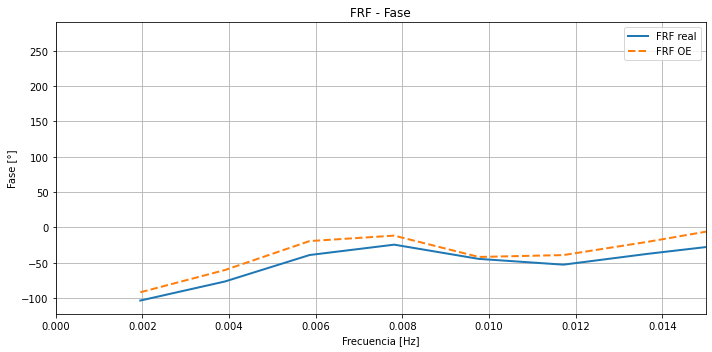
\includegraphics[width=\linewidth]{Figure 2026-05-21 133410 (11).png}
        \caption{Fase de FRF.}
        \label{fig:FRFfsimliOE2}
    \end{subfigure}

    \caption{Análisis de residuos y respuesta en frecuencia del modelo OE en simulación libre.}
    \label{fig:analisis_completo_OE2}
\end{figure}

En conjunto, los resultados muestran que el modelo OE logra capturar parcialmente la dinámica dominante de baja frecuencia del sistema térmico. La similitud observada en la PSD y en la FRF indica que la estructura representa de manera razonable el comportamiento frecuencial principal, especialmente en la zona donde se concentra la mayor parte de la energía de la respuesta térmica. Sin embargo, el desempeño temporal en simulación libre fue inferior al esperado y menor que el obtenido con el segundo modelo ARX. Esto puede explicarse porque el modelo OE concentra la identificación en la dinámica directa entre la entrada y la salida, sin incorporar una estructura autorregresiva asociada a la salida medida, como ocurre en el modelo ARX. Por esta razón, su desempeño depende en mayor medida de que la dinámica entrada-salida quede correctamente representada por los polinomios B(q) y F(q), así como por el retardo seleccionado. La presencia de un sesgo positivo en la temperatura simulada, residuos estructurados y correlación significativa entre la entrada y el error indica que la estructura OE identificada no logró capturar completamente la dinámica térmica del sistema. Además, al tratarse de un sistema de dinámica lenta, pequeños errores en la ganancia estática, en el punto de operación o en el retardo efectivo pueden acumularse durante la simulación libre, provocando una sobrestimación sostenida de la temperatura. Por lo tanto, el menor desempeño del modelo OE no invalida la elección de esta estructura, sino que evidencia que, para este conjunto de datos y configuración identificada, la dinámica del proceso no fue representada con suficiente precisión. En consecuencia, el modelo OE no puede considerarse suficientemente preciso para predicción temporal directa, aunque sí entrega una representación aproximada de la dinámica frecuencial dominante.

Estos resultados permiten avanzar hacia la identificación de una estructura Box-Jenkins. A diferencia del modelo OE, que considera la dinámica entrada-salida pero no modela explícitamente la dinámica del ruido, el modelo Box-Jenkins incorpora de forma separada una dinámica para el proceso y una dinámica para la perturbación o error. Esta característica resulta pertinente en este caso, ya que los residuos obtenidos con el modelo OE presentan una estructura no aleatoria y mantienen correlación con la entrada, lo que sugiere que el error no se comporta como ruido blanco. Por lo tanto, una estructura Box-Jenkins podría mejorar la representación del sistema al permitir modelar simultáneamente la dinámica determinística entre entrada y salida, y la dinámica asociada a las perturbaciones no capturadas.



\subsection{Modelo Box-Jenkins}

A partir de los resultados obtenidos con los modelos ARX y Output-Error, se observa que ambas estructuras logran representar parcialmente la dinámica dominante del sistema térmico. Sin embargo, los análisis de validación muestran que aún persisten limitaciones importantes, principalmente asociadas a la presencia de residuos con estructura, correlaciones significativas entre la entrada y el error, y discrepancias en la representación temporal de la temperatura en simulación libre. Estos resultados sugieren que parte de la dinámica del sistema o de las perturbaciones presentes durante la adquisición de datos, no ha sido modelada adecuadamente mediante las estructuras evaluadas previamente.
En este contexto, se propone evaluar una estructura Box-Jenkins (BJ), debido a su mayor flexibilidad para representar, de forma separada, la dinámica determinística entre la entrada y la salida y la dinámica asociada al error o a las perturbaciones. Esta característica resulta especialmente relevante para el sistema térmico estudiado, ya que los modelos anteriores evidenciaron residuos no aleatorios, lo que indica que el error no corresponde únicamente a ruido blanco, sino que puede contener información dinámica no capturada.

Por lo tanto, la identificación de un modelo Box-Jenkins se plantea con el objetivo de analizar si una estructura más flexible permite mejorar la representación temporal del sistema, reducir la correlación entre entrada y residuos y capturar de mejor manera las dinámicas no modeladas observadas en las validaciones anteriores. 



\subsubsection{Proceso de identificación y selección para el modelo Box-Jenkins}

El proceso de identificación del modelo Box-Jenkins (BJ) se desarrolló mediante una estrategia de exploración y refinamiento de estructuras, siguiendo una lógica similar a la utilizada previamente para los modelos ARX y OE. Sin embargo, el modelo BJ presenta una mayor complejidad, ya que representa de manera independiente la dinámica determinística entrada-salida y la dinámica asociada al error mediante los polinomios $B(q)$, $F(q)$, $C(q)$ y $D(q)$ (Ecuación \ref{ecuacionBJ}). Debido a esta estructura, la estimación de sus parámetros requiere un procedimiento iterativo de optimización no lineal.
\begin{enumerate}


\item \textbf{Preparación y preprocesamiento de los datos}
    
    Para la identificación se utilizaron únicamente los datos posteriores a los primeros 500 segundos, eliminando así el período inicial de estabilización. Las señales de caudal y $\Delta T$ fueron posteriormente normalizadas mediante sus respectivas medias y desviaciones estándar, con el propósito de trabajar con variables en escalas comparables y mejorar el acondicionamiento numérico durante la optimización. Finalmente, el conjunto de datos normalizado se dividió cronológicamente, utilizando el 80 \% inicial para identificación y el 20 \% restante para validación.
    
    \item \textbf{Definición de las estructuras candidatas}

    La estructura de un modelo BJ queda determinada mediante los órdenes $n_b$, $n_f$, $n_c$, $n_d$ y $n_k$. El parámetro $n_b$ determina el número de coeficientes del polinomio $B(q)$, asociado al efecto de entrada sobre la salida; $n_f$ establece el orden del polinomio $F(q)$, correspondiente a la dinámica determinística del sistema; $n_c$ y $n_d$ definen los órdenes de los polinomios $C(q)$ y $D(q)$, utilizados para representar la dinámica del error. Finalmente, $n_k$ corresponde al retardo discreto entre la entrada y la salida. A partir de estos parámetros se definió una malla de combinaciones posibles.

La búsqueda se realiza evaluando una combinación de órdenes a la vez. Por ejemplo, al seleccionar temporalmente determinados valores de $n_b$, $n_f$, $n_c$, $n_d$ y $n_k$, queda definida la cantidad de coeficientes que deben estimarse para cada polinomio. Solo entonces se procede a calcular los parámetros correspondientes a esa estructura. Una vez identificada y evaluada, el procedimiento continúa con la siguiente combinación de órdenes de la malla.

    

\item \textbf{Inicialización de los parámetros}

Antes de comenzar la optimización no lineal, se obtuvo una estimación inicial de los coeficientes asociados a la parte determinística del modelo, correspondiente a los polinomios $B(q)$ y $F(q)$. Para ello se utilizó una aproximación tipo ARX estimada mediante mínimos cuadrados lineales. Los coeficientes obtenidos se emplearon como punto inicial para la posterior identificación BJ. En cambio, los coeficientes de $C(q)$ y $D(q)$, asociados al modelo del error, se inicializaron en cero. A partir de estos valores, el algoritmo de mínimos cuadrados no lineales ajusta iterativamente los coeficientes de los cuatro polinomios hasta reducir el error de predicción.
Esta estrategia proporciona al optimizador una condición inicial razonable para la dinámica entrada-salida y facilita la convergencia del procedimiento iterativo.


\item \textbf{Estimación iterativa de los parámetros}


A partir de los valores iniciales definidos en la etapa anterior, los coeficientes de $B(q)$, $F(q)$, $C(q)$ y $D(q)$ se estimaron mediante mínimos cuadrados no lineales. Para cada conjunto de coeficientes propuesto durante la optimización, se calculó primero la salida del modelo a partir de la entrada utilizando la relación $B(q)/F(q)$. Esta salida se comparó con la salida medida del sistema, obteniéndose una señal de error.
Posteriormente, esta señal de error fue procesada mediante la relación $D(q)/C(q)$, la cual incorpora la dinámica asociada al modelo del ruido. De esta forma se obtiene el error de predicción utilizado por el algoritmo como criterio de ajuste. El optimizador modifica iterativamente los coeficientes de los cuatro polinomios buscando reducir dicho error hasta alcanzar una solución para la estructura evaluada.

Durante esta etapa también se incorporó una penalización cuando las raíces de los polinomios se ubicaban fuera del círculo unitario, con el propósito de evitar estructuras con comportamiento inestable.

\item \textbf{Evaluación de cada estructura candidata}
    
    Una vez estimados los parámetros, cada modelo fue evaluado mediante simulación libre sobre el conjunto de validación. Para esta simulación se utilizó únicamente la parte determinística B(q)/F(q), ya que el objetivo es analizar la capacidad del modelo para reproducir la evolución del sistema a partir de la entrada conocida, sin incorporar la realización particular del ruido presente en los datos experimentales. El desempeño se cuantificó mediante RMSE, MAE, $R^2$ y FIT.

 \item \textbf{Criterio de selección de los modelos}

 
La selección de las estructuras no se realizó únicamente a partir del error obtenido en simulación. Para cada candidato se calculó el criterio de información bayesiano (BIC), que penaliza el aumento de la cantidad de parámetros cuando este no se traduce en una mejora suficiente del ajuste. Además, se calculó una penalización asociada a la correlación entre la entrada y el error de predicción. La función de costo utilizada combina ambos criterios, favoreciendo modelos con menor complejidad y con residuos menos relacionados con la señal de entrada.

\item \textbf{Búsqueda preliminar y refinamiento de la estructura}

La malla de órdenes definida previamente para $n_b$, $n_f$, $n_c$, $n_d$ y $n_k$ se utilizó como primera etapa de búsqueda. En ella se evaluaron todas las combinaciones consideradas, pero con un número limitado de iteraciones del algoritmo de optimización, con el propósito de reducir el costo computacional y localizar una primera estructura favorable. Una vez finalizada esta búsqueda, se seleccionó la combinación de órdenes que presentó el menor valor de la función de costo.

A partir de ese modelo preliminar se construyó una segunda malla, ahora más acotada, formada por valores cercanos a los órdenes seleccionados en la primera etapa. Cada una de estas nuevas combinaciones fue nuevamente identificada y evaluada, permitiendo un mayor número de iteraciones durante la optimización de sus parámetros. De esta manera, la primera malla permitió explorar de forma general el espacio de estructuras, mientras que la segunda permitió realizar una búsqueda más detallada alrededor de la región que había mostrado el mejor desempeño.

    \item \textbf{Selección y evaluación final}
    
  Finalmente, se comparó el mejor modelo obtenido en la búsqueda preliminar con el mejor modelo obtenido durante el refinamiento, seleccionándose aquel que presentó el menor valor de la función de costo. Con la estructura y los coeficientes definitivos se realizó una simulación libre. La respuesta fue posteriormente reconstruida en la escala original y se calcularon los indicadores finales RMSE, MAE, $R^2$ y FIT. 
\end{enumerate}

En conjunto, este procedimiento permite seleccionar la estructura Box-Jenkins considerando simultáneamente la representación de la dinámica entrada-salida, el comportamiento del error, la complejidad del modelo y su capacidad de simulación. La estrategia de búsqueda preliminar seguida de un refinamiento local permite además reducir el costo computacional asociado a la exploración de las cinco dimensiones estructurales $n_b$, $n_f$, $n_c$, $n_d$ y $n_k$.

Como resultado del procedimiento de búsqueda y refinamiento descrito anteriormente, se seleccionó la siguiente estructura Box-Jenkins:
\begin{itemize}
    \item $n_b=1$
    \item $n_f=2$
    \item $n_c=2$
    \item $n_d=3$
    \item $n_k=8$
\end{itemize}
Estos órdenes no fueron establecidos previamente, sino que corresponden a la combinación que presentó el mejor desempeño dentro de las estructuras evaluadas según la función de costo definida. Por lo tanto, su selección considera conjuntamente la calidad del ajuste, la complejidad de la estructura y la relación existente entre la entrada y los residuos. De esta manera, los valores obtenidos representan el mejor compromiso encontrado dentro del espacio de búsqueda analizado.


Los parámetros $n_b$ y $n_f$ determinan la estructura de la relación entre la entrada y la salida. En particular $n_b=1$ indica que el polinomio $B(q)$ está constituido por un único coeficiente, por lo que el efecto del caudal queda representado mediante un término de entrada retardado. Este resultado muestra que, dentro de las estructuras evaluadas, no fue necesario incorporar un mayor número de coeficientes en el numerador para obtener el mejor compromiso entre desempeño y complejidad.

Por su parte, $n_f=2$ establece un polinomio denominador $F(q)$ de segundo orden. Este polinomio determina la evolución dinámica de la salida generada por el modelo y permite incorporar la memoria necesaria para representar la respuesta temporal del sistema. La selección de un segundo orden indica que, dentro de la búsqueda realizada, aumentar la complejidad del denominador no produjo una mejora suficiente como para justificar la incorporación de parámetros adicionales.

El parámetro $n_k=8$ corresponde al retardo discreto seleccionado entre la entrada y la salida. Considerando un período de muestreo de $T_s=2$ segundos, este valor equivale a aproximadamente 16 segundos. Esto significa que, en la estructura identificada, la influencia del caudal comienza a incorporarse en la salida modelada después de ocho muestras. Al igual que los demás órdenes, este valor corresponde al resultado del procedimiento de identificación y no a una medición directa del tiempo físico de transporte del sistema.

Los órdenes de $n_c=2$ y $n_d=3$ determinan, en cambio, la estructura utilizada para representar la dinámica del error. El valor $n_c=2$ establece dos coeficientes en el polinomio $C(q)$, mientras que $n_d=3$ define un polinomio $D(q)$ de tercer orden. Esta combinación permite que el modelo Box-Jenkins represente temporalmente aquella parte de la salida que no es explicada únicamente por la relación entre el caudal y la temperatura. La selección de estos órdenes también fue determinada por el procedimiento de búsqueda, favoreciendo la estructura que logró mejorar la descripción del error sin incorporar una complejidad excesiva.


De esta forma, la estructura seleccionada separa la representación de la dinámica entrada-salida, definida por $B(q)/F(q)$, de la dinámica asociada al error, representada por $C(q)/D(q)$. Esta característica constituye la principal diferencia respecto de las estructuras ARX y OE evaluadas anteriormente y resulta de especial interés debido a la presencia de residuos estructurados observada en los modelos previos.

Para la estructura seleccionada, los polinomios identificados fueron:


$$B(q)=−0.04403592$$
$$F(q)=1−0.2968672q^{−1}−0.68409118q^{−2}$$
$$C(q)=1−0.16956181q^{−1}−0.55284664q^{−2}$$
$$D(q)=1−0.95506241q^{−1}−0.91586418q^{−2}+0.87617206q^{−3}$$

A partir de estos polinomios, la relación $B(q)/F(q)$ describe la respuesta modelada asociada a la entrada de caudal, mientras que $C(q)/D(q)$ representa la dinámica atribuida al error. Por lo tanto, el modelo BJ seleccionado dispone de una estructura relativamente simple para representar la relación entrada-salida y de una estructura adicional para describir las componentes del error que presentan dependencia temporal.

\begin{comment}
    

\begin{figure}[H]
    \centering
    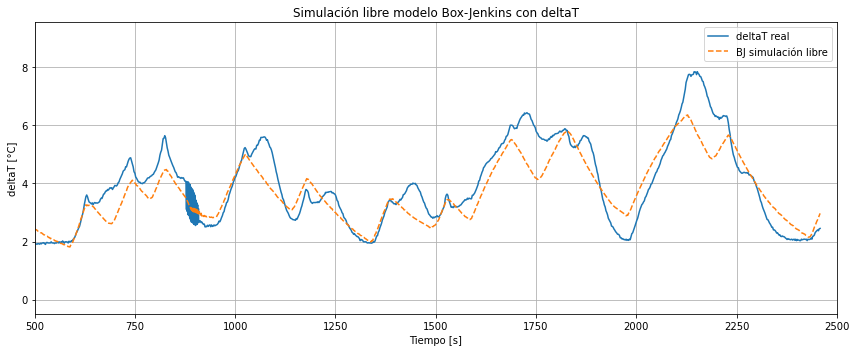
\includegraphics[width=0.65\linewidth]{ModeloBJ.png}
    \caption{Modelo BJ simulado al momento de su identificación.}
    \label{fig:modeloBJ}
\end{figure}
\end{comment}


\subsubsection{Simulación Libre}

La simulación libre del modelo Box-Jenkins se realizó siguiendo el mismo criterio utilizado en las estructuras anteriores. Para reconstruir la salida del modelo, expresada como variación de temperatura, se consideró una temperatura base igual a la temperatura ambiente registrada durante la adquisición de los datos. De esta manera, la respuesta simulada fue transformada a temperatura absoluta para ser comparada con la temperatura real del sistema.

La Figura \ref{fig:SimulacionlibreBJ} muestra la comparación entre la temperatura real y la respuesta obtenida mediante el modelo Box-Jenkins en simulación libre. Se observa que el modelo reproduce de manera adecuada la forma general de la curva, logrando incluso aproximarse a la temperatura real en algunos intervalos, especialmente entre los 3000 y 3500 segundos. Sin embargo, durante gran parte del registro, la respuesta simulada tiende a sobrestimar la temperatura del sistema. Esto indica que, si bien la estructura BJ mejora ciertos aspectos de la representación dinámica, aún existe un sesgo en la respuesta temporal.
\begin{figure}[H]
    \centering
    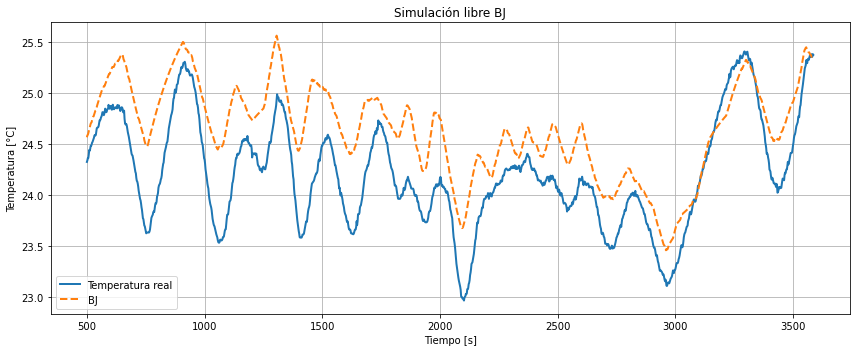
\includegraphics[width=0.5\linewidth]{Figure 2026-05-26 112051 (0).png}
    \caption{Simulación libre del modelo Box-Jenkins}
    \label{fig:SimulacionlibreBJ}
\end{figure}
Los indicadores temporales obtenidos son:
\begin{itemize}
    \item RMSE                 = 0.504064 °C
\item MAE                  = 0.441288 °C
\item $R^2$                   = 0.082809
\item FIT                  = 4.230 \%
\end{itemize}
En comparación con los modelos ARX y OE evaluados previamente, el modelo Box-Jenkins presenta un mejor desempeño en términos de error absoluto, ya que tanto el RMSE como el MAE se mantienen cercanos o inferiores a 0.5 °C. Esto indica que la magnitud promedio del error se redujo. No obstante, el valor de $R^2$, cercano a cero, muestra que el modelo explica solo una fracción reducida de la variabilidad total de la temperatura real. De manera similar, el bajo valor de FIT confirma que la estructura identificada no logra reproducir adecuadamente la evolución temporal completa del sistema en simulación libre.

El análisis de residuos, presentado en la Figura \ref{fig:ResiduosBJ}, evidencia que el error no presenta un comportamiento completamente aleatorio. Los residuos oscilan aproximadamente entre -1 °C y 0.2 °C, manteniendo una estructura definida a lo largo del tiempo. Esto indica que el error no se comporta como ruido blanco y que todavía existen componentes dinámicas que no han sido capturadas completamente por el modelo.

La correlación cruzada entre la entrada y los residuos, mostrada en la Figura \ref{fig:CorrelacionBJ}, presenta valores significativos, especialmente para retardos positivos. Este resultado indica que parte de la información asociada al caudal aún permanece en el error del modelo. En consecuencia, la estructura Box-Jenkins no logra representar completamente la relación dinámica entre el caudal y la temperatura de salida, a pesar de incorporar una dinámica separada para el error.

La densidad espectral de potencia, observada en la Figura \ref{fig:PSDbj}, muestra una forma y magnitud similares a la respuesta real del sistema, aunque con menor energía en algunas bandas de frecuencia. Esto sugiere que el modelo captura parte del contenido energético dominante de la salida, especialmente en la zona de bajas frecuencias, donde se concentra la dinámica térmica principal.

En cuanto a la función de respuesta en frecuencia, la magnitud de la FRF, presentada en la Figura \ref{fig:FRFMbj}, reproduce parcialmente la pendiente global del sistema, pero no sigue con precisión todas las variaciones de ganancia. Por otra parte, la fase de la FRF, mostrada en la Figura \ref{fig:FRFFBj}, presenta cierta concordancia en frecuencias muy bajas; sin embargo, se observan diferencias relevantes en el resto de la banda analizada. Esto indica que el modelo logra representar parcialmente la dinámica dominante del sistema, pero no reproduce completamente el retardo efectivo ni la distribución dinámica asociada a la respuesta térmica.

\begin{figure}[H]
    \centering

    % --- Fila 1: Residuos ---
    \begin{subfigure}[b]{0.48\textwidth}
        \centering
        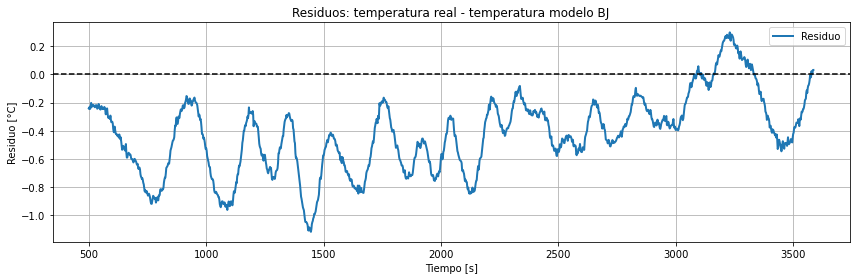
\includegraphics[width=\linewidth]{Figure 2026-05-26 112051 (4).png}
    \caption{Residuos de la simulación libre del modelo BJ.}
    \label{fig:ResiduosBJ}
    \end{subfigure}
    \hfill % Espacio horizontal entre subfiguras
    \begin{subfigure}[b]{0.48\textwidth}
        \centering
        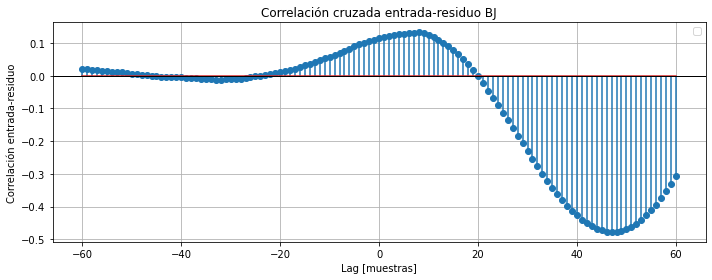
\includegraphics[width=\linewidth]{Figure 2026-05-26 112051 (7).png}
    \caption{Correlación entre la entrada y los residuos del modelo.}
        \label{fig:CorrelacionBJ}
    \end{subfigure}

    \vspace{1em} % Espacio vertical entre filas

    % --- Fila 2: PSD y Magnitud FRF ---
    \begin{subfigure}[b]{0.48\textwidth}
        \centering
        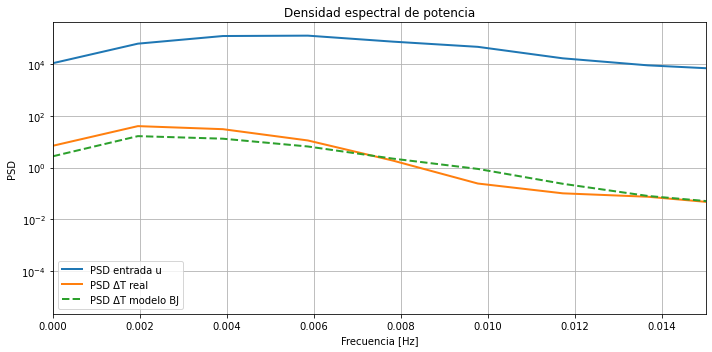
\includegraphics[width=\linewidth]{Figure 2026-05-26 112051 (8).png}
    \caption{Comparación de densidad espectral real y del modelo.}
    \label{fig:PSDbj}
    \end{subfigure}
    \hfill
    \begin{subfigure}[b]{0.48\textwidth}
        \centering
        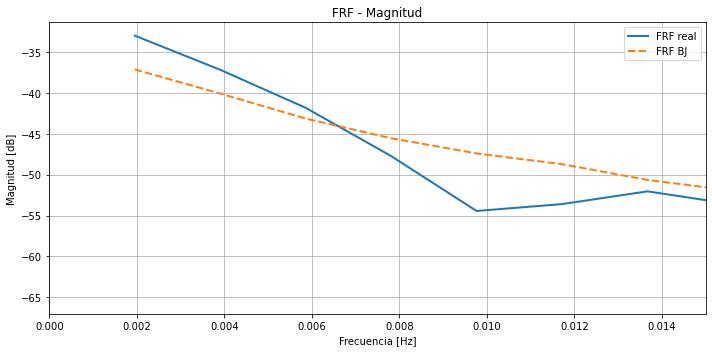
\includegraphics[width=\linewidth]{Figure 2026-05-26 112051 (10).png}
    \caption{Magnitud FRF}
    \label{fig:FRFMbj}
    \end{subfigure}

    \vspace{1em} % Espacio vertical entre filas

    % --- Fila 3: Fase FRF (centrada) ---
    \begin{subfigure}[b]{0.48\textwidth}
        \centering
        % La última imagen se mantendrá a la izquierda si no se hace nada.
        % Al usar un ancho total de 1 y centrar la figura, 
        % esta imagen se centrará en la fila.
        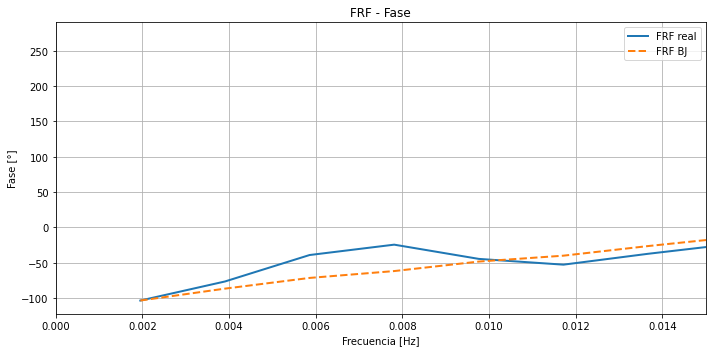
\includegraphics[width=\linewidth]{Figure 2026-05-26 112051 (11).png}
    \caption{Fase FRF}
    \label{fig:FRFFBj}
    \end{subfigure}
    % Se deja vacío el espacio de la derecha para centrar la última imagen

    % --- Título General ---
    \caption{Resultados del análisis y validación del modelo Box-Jenkins.}
    \label{fig:ResultadosCompletosBJ}

\end{figure}

En síntesis, la simulación libre del modelo Box-Jenkins muestra una mejora respecto a las estructuras ARX y OE en términos de error absoluto, alcanzando valores menores de RMSE y MAE. Sin embargo, el bajo valor de FIT, el $R^2$ cercano a cero, la estructura presente en los residuos y la correlación significativa entre entrada y error evidencian que el modelo aún no reproduce completamente el comportamiento real del sistema. Por lo tanto, aunque el modelo BJ representa parcialmente la dinámica dominante de baja frecuencia, su capacidad de predicción temporal directa sigue siendo limitada.

\subsection{Comparación de modelos lineales SISO}

En esta sección se comparan los modelos SISO lineales identificados. Las estructuras evaluadas corresponden a los dos modelos ARX, el modelo Output-Error y el modelo Box-Jenkins.
El primer modelo ARX fue identificado utilizando directamente la temperatura absoluta como variable de salida, mientras que los otros tres modelos fueron desarrollados considerando la salida en forma de variación de temperatura, reconstruida posteriormente a temperatura absoluta para su comparación.

A partir de los indicadores temporales obtenidos, se observa que el primer modelo ARX presentó el desempeño más bajo entre todas las estructuras evaluadas. Este modelo obtuvo un RMSE de 8.6566 °C, un MAE de 8.6491 °C, un valor de $R^2$ fuertemente negativo y un FIT de -1539.13 \% (Tabla \ref{tab:metricas_modelos}). Estos resultados evidencian que la identificación directa sobre la temperatura absoluta no permitió representar adecuadamente la dinámica del sistema en simulación libre. En particular, el elevado error obtenido indica que el modelo no fue capaz de reproducir correctamente el nivel ni la evolución temporal de la temperatura. Esto puede estar asociado a la influencia del punto de operación térmico, las condiciones iniciales y las diferencias ambientales presentes entre los datos de identificación y validación.

El segundo modelo ARX, identificado utilizando la salida en forma de variación de temperatura, presentó una mejora significativa respecto al primer modelo. En este caso, el RMSE disminuyó a 0.623598 °C y el MAE a 0.598302 °C (Tabla \ref{tab:metricas_modelos}), lo que muestra que trabajar con $\Delta T$ permitió reducir considerablemente la magnitud del error. Además, este modelo presentó una mayor similitud en la PSD y en la FRF respecto de las obtenidas experimentalmente dentro de la banda de frecuencias de interés, indicando que logró capturar parte de la dinámica dominante del sistema, especialmente en bajas frecuencias. Sin embargo, los valores negativos de $R^2$ y FIT, que se observan en la Tabla \ref{tab:metricas_modelos}, muestran que, en simulación libre, el modelo no reproduce adecuadamente la evolución temporal completa de la temperatura. Esto es coherente con la naturaleza de la estructura ARX, ya que su formulación acopla la dinámica del sistema y la dinámica del error en un mismo polinomio, lo que puede afectar su desempeño cuando el modelo debe generar sus propias salidas sin retroalimentación con mediciones reales.

El modelo OE fue evaluado con el objetivo de mejorar el desempeño en simulación libre, debido a que esta estructura modela explícitamente la dinámica determinística del proceso y no incorpora un modelo dinámico independiente para el ruido. Sin embargo, los resultados obtenidos muestran que el modelo OE presentó un desempeño temporal inferior al segundo modelo ARX. Aunque la curva simulada siguió parcialmente la forma general de la temperatura real, se observó una sobrestimación sistemática de la salida, reflejada en residuos mayoritariamente negativos. Esto se tradujo en un RMSE de 0.819204 °C, un MAE de 0.796064 °C, un $R^2$ de -1.422553 y un FIT de -55.646 \% (Tabla \ref{tab:metricas_modelos}). Por lo tanto, para la estructura y los datos utilizados en este caso, el modelo OE no logró mejorar la representación temporal del sistema en simulación libre.

De acuerdo con los criterios utilizados, el modelo Box-Jenkins presentó el mejor desempeño entre las estructuras lineales SISO evaluadas. Este obtuvo el menor error cuadrático medio, con un RMSE de 0.504064 °C, y el menor error absoluto medio, con un MAE de 0.441288 °C. Además, fue el único modelo que entregó valores positivos de $R^2$ y FIT, aunque ambos indicadores fueron bajos, con valores de 0.082809 y 4.230 \%, respectivamente (Tabla \ref{tab:metricas_modelos}). Estos resultados indican que el modelo BJ logró reducir la magnitud promedio del error respecto de las demás estructuras evaluadas, aunque todavía no explica de manera satisfactoria la variabilidad temporal completa de la temperatura.

El mejor desempeño relativo del modelo BJ puede atribuirse a su estructura más flexible. A diferencia de los modelos ARX y OE, el modelo Box-Jenkins representa separadamente la dinámica determinística entre la entrada y la salida mediante la relación B(q)/F(q), y la dinámica asociada al error mediante C(q)/D(q). Esta separación resulta relevante en el sistema térmico estudiado, ya que los modelos previamente evaluados mostraron residuos con estructura, lo que sugiere que el error no se comporta como ruido blanco, sino que contiene información dinámica no modelada. En este sentido, la estructura BJ permite representar de mejor manera sistemas donde existen perturbaciones no medidas, variaciones ambientales, ruido de sensores o efectos térmicos no completamente explicados por la entrada considerada.

En resumen, el modelo Box-Jenkins fue seleccionado como la mejor estructura lineal SISO entre las evaluadas, debido a que presentó los menores errores temporales y los mejores valores de $R^2$ y FIT. Sin embargo, aunque este modelo mejora el desempeño respecto de las estructuras ARX y OE, sus indicadores globales siguen siendo bajos. Por lo tanto, el modelo BJ representa la mejor alternativa dentro del conjunto de modelos lineales SISO analizados, pero no constituye una solución suficientemente precisa para la predicción temporal directa en simulación libre.


%El resultados de los indicadores temporales se pueden ver en la Tabla \ref{tab:metricas_modelos}:


\begin{table}[H]
\centering
\begin{tabular}{|l|l|l|l|l|}
\hline
\textbf{Modelo} & \textbf{RMSE (°C)} & \textbf{MAE (°C)} & \textbf{$R^2$} & \textbf{FIT} \\ \hline
\textbf{ARX 1}  & 8.6566           & 8.6491          & -267.6743                     & -1539.13\%  \\ \hline
\textbf{ARX 2}  & 0.623598           & 0.598302          & -0.403776                     & -18.481\%  \\ \hline
\textbf{OE}     & 0.819204           & 0.796064          & -1.422553                     & -55.646\%  \\ \hline
\textbf{BJ}     & 0.504064           & 0.441288          & 0.082809                      & 4.230\%    \\ \hline
\end{tabular}
\caption{Comparación de métricas temporales para los modelos ARX, OE y BJ.} 
\label{tab:metricas_modelos}
\end{table}



\subsection{Limitaciones de los modelos lineales SISO}

A pesar de que el modelo Box-Jenkins presentó el mejor desempeño relativo entre las estructuras lineales SISO evaluadas, los resultados de validación muestran que ninguno de los modelos logró reproducir completamente la evolución temporal de la temperatura en simulación libre. En términos generales, los modelos lograron representar parcialmente la dinámica dominante de baja frecuencia del sistema, lo que se evidenció en la similitud observada en la PSD y, en algunos casos, en la FRF. Sin embargo, en el dominio temporal los valores de $R^2$ y FIT fueron bajos o negativos, y los residuos presentaron una estructura no aleatoria.

Desde el punto de vista de la validación de modelos, este resultado es destacable, ya que un modelo adecuado debe generar residuos aproximadamente blancos y no correlacionados con la entrada \cite{ljung1999system}. En los modelos evaluados, los residuos mantuvieron una estructura definida y la correlación cruzada entre la entrada y el residuo presentó valores significativos para distintos retardos. Esto indica que los residuos aún contienen información dinámica asociada a la entrada, por lo que las estructuras lineales SISO evaluadas no capturan completamente la relación entre el caudal y la temperatura del sistema.

El bajo desempeño temporal puede estar asociado a distintas causas. En primer lugar, el sistema térmico puede presentar comportamientos no lineales. Las pérdidas ambientales, los fenómenos de transferencia de calor, la respuesta térmica de los paneles y la relación entre caudal y temperatura pueden variar según el punto de operación. En consecuencia, una estructura lineal SISO puede resultar insuficiente para representar completamente la dinámica del sistema, especialmente cuando la respuesta térmica depende de condiciones operacionales cambiantes.

Además, en este trabajo los modelos fueron identificados y validados bajo condiciones térmicas diferentes. En particular, los modelos fueron identificados con datos obtenidos en verano y validados con datos adquiridos en invierno. Esto introduce diferencias relevantes en las condiciones de operación, tales como cambios en la temperatura ambiente del laboratorio, en la temperatura de entrada del agua a los paneles y en las pérdidas térmicas hacia el entorno. Estas variaciones no dependen únicamente de la señal de entrada aplicada, por lo que no pueden ser completamente representadas por un modelo SISO que considere solo el caudal como entrada.

Asimismo, el bajo desempeño puede deberse a que la dinámica real del sistema no queda completamente descrita mediante una única variable de entrada. En el caso del banco experimental estudiado, el uso exclusivo del caudal como entrada puede resultar insuficiente, ya que la temperatura de salida también se ve influenciada por otras variables, como la potencia térmica entregada por las resistencias, la temperatura ambiente y la temperatura de entrada del fluido. Por ello, una estructura MISO puede representar de manera más completa el comportamiento del sistema, al incorporar simultáneamente más de una variable que incide sobre la salida.

La necesidad de evaluar modelos no lineales también se justifica por la presencia de residuos estructurados, sesgos sostenidos y discrepancias en la representación temporal de la temperatura. Estos elementos sugieren que la relación entre la entrada y la salida podría no ser completamente lineal dentro del rango de operación analizado. En sistemas térmicos, este comportamiento puede originarse por la dependencia de los coeficientes de transferencia de calor respecto del caudal, las pérdidas térmicas hacia el ambiente, la acumulación de energía en los paneles y la interacción entre las variables de operación.

En consecuencia, aunque el modelo Box-Jenkins fue la mejor estructura lineal SISO evaluada, su desempeño sigue siendo limitado para reproducir con precisión la temperatura en simulación libre. Los modelos lineales SISO permitieron representar parcialmente la dinámica dominante de baja frecuencia, pero no capturaron completamente el comportamiento temporal del sistema ni eliminaron la información dinámica presente en los residuos.

Por esta razón, la siguiente etapa del estudio debe orientarse hacia la identificación de modelos MISO, incorporando más de una entrada al modelo, particularmente el caudal y la potencia eléctrica entregada por las resistencias. Esta formulación permite representar de manera más completa el balance energético del banco de ensayos, considerando simultáneamente el efecto del transporte de energía asociado al flujo de agua y el aporte térmico suministrado al sistema. Además, debido a las limitaciones observadas en las estructuras lineales, también resulta pertinente evaluar modelos no lineales, capaces de representar interacciones más complejas entre las entradas y la salida. De esta manera, se busca mejorar la simulación libre, reducir la correlación entre entrada y residuos, y obtener una representación más precisa de la dinámica térmica del sistema.






\begin{comment}
    


\subsection{Conclusión de la validación de modelos lineales}
Desde el punto de vista de la validación de modelos, este resultado es relevante, ya que, de acuerdo con Ljung \cite{ljung1999system}, un modelo adecuado debe generar residuos aproximadamente blancos y no correlacionados con la entrada. En los modelos evaluados, los residuos mantienen una estructura definida y la correlación cruzada entrada-residuo presenta valores significativos para distintos retardos. Esto indica que los residuos aún contienen información dinámica asociada a la entrada, por lo que las estructuras lineales evaluadas no capturan completamente la relación entre el caudal y la temperatura del sistema.

El bajo desempeño temporal puede estar asociado a distintas causas. En primer lugar, el sistema térmico puede presentar comportamientos no lineales, ya que las pérdidas ambientales, los fenómenos de transferencia de calor, la respuesta térmica de los paneles y la relación entre caudal y temperatura pueden variar según el punto de operación. Además, en este trabajo los modelos fueron identificados con datos obtenidos en verano y validados con datos experimentales adquiridos en invierno, lo que introduce diferencias relevantes en las condiciones de operación. En particular, cambia la temperatura de entrada del agua a los paneles y la temperatura ambiente del laboratorio, generando variaciones que no dependen únicamente de la señal de entrada aplicada al sistema.

Asimismo, el bajo desempeño puede deberse a que la dinámica real del sistema no queda completamente representada mediante una estructura SISO. En este sentido, en \cite{BARTHELEMY2025109971} muestran que en sistemas térmicos la incorporación de más entradas en una estructura MISO puede mejorar el desempeño del modelo, al representar de mejor manera las condiciones térmicas de frontera del sistema. En el caso del banco experimental estudiado, el uso exclusivo del caudal como entrada puede resultar insuficiente para describir completamente la evolución de la temperatura, ya que no se consideran explícitamente variables como la potencia térmica, la temperatura ambiente o la temperatura de entrada del fluido.

La presencia de dinámica no modelada también puede estar relacionada con una estructura no lineal del sistema. Esto es coherente con lo reportado en \cite{mechaqrane2004comparison}, quienes compararon un modelo ARX lineal con un modelo no lineal NARX para la predicción de temperatura interior, observando que el modelo no lineal redujo considerablemente el error respecto del ARX lineal. Esto sugiere que, en sistemas térmicos, la limitada capacidad de los modelos lineales puede estar asociada a la presencia de relaciones no lineales entre las variables de entrada y salida.

En consecuencia, se concluye que el modelo Box-Jenkins fue la mejor estructural lineal entre las evaluadas, debido a que presentó menores errores temporales y los mejores valores de FIT y $R^2$. No obstante, su desempeño sigue siendo limitado, por lo que no puede considerarse un modelo suficientemente preciso para predicción temporal directa en simulación libre. Los modelos lineales identificados permiten representar parcialmente la dinámica dominante de baja frecuencia del sistema térmico, pero no logran capturar completamente su comportamiento temporal.

Finalmente, el bajo desempeño observado puede estar asociado a la no linealidad del sistema, a la ausencia de variables de entrada relevantes o condiciones térmicas internas, así como retardos y variaciones del punto de operación. Por esta razón, la siguiente etapa del estudio debe orientarse hacia una estructura MISO, incorporando más de una entrada al modelo y eventualmente hacia estructuras no lineales con el objetivo de mejorar la representación dinámica del sistema térmico en simulación libre.
\end{comment}



\begin{comment}
\begin{table}[H]
\centering
\begin{tabular}{|l|l|l|l|}
\hline
\textbf{Modelo} & \textbf{Estructura} & \textbf{Órdenes}                                                          & \textbf{Retardos} \\ \hline
\textbf{ARX 3}  &       $y(k)=\frac{B(q)}{A(q)}u(k)+\frac{1}{A(q)}e(k)$              & \begin{tabular}[c]{@{}l@{}}$n_a=17$ \\ $n_b=21$\end{tabular}                & $n_k=9$            \\ \hline
\textbf{OE}     & $y(k)=\frac{B(q)}{F(q)}u(k)+e(k)$           & \begin{tabular}[c]{@{}l@{}}$n_f=3$\\ $n_b=9$\end{tabular}                   & $n_k$=7            \\ \hline
\textbf{BJ}     & $y(k)=\frac{B(q)}{F(q)}u(k)+\frac{C(q)}{D(q)}e(k)$            & \begin{tabular}[c]{@{}l@{}}$n_f=2$\\ $n_b=1$\\ $n_c=2$\\ $n_d=3$\end{tabular} & $n_k=8$            \\ \hline
\end{tabular}
\caption{Estructura de los modelos ARX, OE y JB.} 
\label{tab:comparacionmodelos}
\end{table}

\end{comment}







\section{Pruebas experimentales con estructura MISO }


Posteriormente, se realizaron ensayos experimentales en los que el caudal de circulación y la potencia suministrada por las resistencias eléctricas fueron excitados simultáneamente. De este modo, el banco de ensayo pasó a ser considerado como un sistema de múltiples entradas y una salida (MISO), cuyas entradas corresponden al caudal y a la potencia eléctrica, mientras que la temperatura medida a la salida del cuarto colector constituye la variable de salida.

La finalidad de estos ensayos fue obtener un conjunto de datos suficientemente informativos para identificar la contribución dinámica de ambas entradas sobre la respuesta térmica del sistema. Para facilitar la diferenciación de sus efectos, se utilizaron señales de excitación de distinta naturaleza: una señal multisinusoidal para el caudal y una señal binaria pseudoaleatoria (PRBS) para la potencia de las resistencias eléctricas. Esta elección permite que ambas entradas presenten estructuras temporales y espectrales diferentes, disminuyendo la posibilidad de que sus efectos sobre la temperatura resulten indistinguibles durante el proceso de identificación.



%Se usó una señal multisinusoidal para excitar al caudal. Esta fue diseñada siguiendo la misma estructura identificada para las pruebas exploratorias anteriores. Sin embargo, según recomendaciones de \cite{ljung1999system}, es importante observar al menos 3 periodos, para identificar un comportamiento periódico en la salida, por lo tanto, el tiempo del experimento aumento a hora y media, 5400 segundos. Sumado a esto, el sistema se estabiliza en 500 segundos, aproximadamente. Así, las pruebas duraron un total de 5900 segundos.
%La potencia de las resistencias eléctricas varío de encendido a apagado, para lo cual se usó una señal PRBS, debido a su característica binaria. Los parámetros para el diseño de esta señal fueron variados, según los experimentos anteriores, para que el periodo de este coincidiera con el periodo de la señal multisinusoidal y se pudieran obtener la misma cantidad de muestras en un periodo. 

%El diseño de ambas señales se realizó bajo un límite de correlación entregado por \cite{csurcsia2020user}, el cual recomienda una correlación menor a 0.8 para que no dependan una de la otra y se puede obtener datos informativos. La idea principal es que ambas señales sean ortogonales, es decir, con correlación 0, lo cual es difícil de conseguir.

\subsection{Diseño de la señal multisinusoidal de caudal}

El caudal fue excitado mediante una señal multisinusoidal periódica, obtenida a partir de la superposición de varias componentes sinusoidales dentro de la banda de frecuencias de interés del sistema. Se mantuvo la estructura utilizada en los experimentos SISO anteriores, considerando frecuencias comprendidas entre 0.0005 y 0.01 Hz.

El tiempo de muestreo y la cantidad de muestras por períodos se mantuvo en 2 segundos y en 900, respectivamente. Por lo tanto, cada período tuvo una duración de 1800 segundos, equivalente a 30 minutos. Con estos parámetros, la resolución frecuencial de la señal fue aproximadamente 0.000556 Hz, lo que permitió incluir un número suficiente de componentes dentro de la banda definida para el experimento.

De acuerdo con las recomendaciones de \cite{ljung1999system}, para analizar adecuadamente una respuesta obtenida mediante señales periódicas es conveniente observar al menos tres períodos completos. La utilización de varios períodos permite comprobar si la salida tiende hacia un comportamiento periódico, evaluar la repetibilidad del experimento y diferenciar la respuesta provocada por las entradas de los efectos producidos por ruido, perturbaciones o condiciones iniciales. %Así, el primer período puede estar afectado por el transitorio térmico inicial del sistema. La comparación entre el segundo y el tercer período permite verificar si la respuesta de temperatura tiende a repetirse cuando se aplica la misma señal de entrada

Antes de aplicar las señales de excitación, el sistema se mantuvo durante aproximadamente 500 segundos bajo condiciones iniciales. Este intervalo permitió reducir la influencia de los transitorios asociados al arranque del banco y establecer una referencia térmica inicial. Considerando los 500 segundos de estabilización y los 5400 segundos de excitación, cada ensayo tuvo una duración total aproximada de 5900 segundos.

Para el primer experimento MISO, la señal multisinusoidal se aplicó con una amplitud de variación de 150, 100 y 50 L/h. Esta amplitud fue seleccionada con el propósito de generar cambios observables en la temperatura, manteniendo al mismo tiempo el sistema dentro de sus límites normales de operación.

Las fases de las componentes sinusoidales fueron definidas utilizando fases de Schroeder. Este procedimiento permite reducir el factor de cresta de la señal, evitando que la superposición de varias componentes produzca valores máximos excesivos. Así, la energía de excitación se distribuye de manera uniforme y se aprovecha mejor el rango disponible del actuador de caudal \cite{ljung1999system}.





\subsection{Diseño de la señal PRBS de potencia eléctrica}

La potencia suministrada por las resistencias eléctricas fue excitada mediante una señal PRBS binaria, debido a que estas operan únicamente en dos estados: apagadas y encendidas. En la señal utilizada, el valor 0 representó el estado apagado y el valor 1 representó el estado encendido.

La PRBS resulta apropiada para este tipo de entrada porque genera una sucesión de cambios binarios con apariencia pseudoaleatoria y con un contenido frecuencial distribuido en un rango amplio. Esto favorece la excitación de diferentes dinámicas del sistema térmico sin requerir valores intermedios de potencia.

La PRBS fue generada mediante un registro de desplazamiento de longitud máxima de orden 5. Para este tipo de secuencia, la cantidad de bits distintos antes de que la señal comience a repetirse está determinada por $M=2^n-1$. Por lo tanto, al utilizar un orden igual a 5 se obtuvo una secuencia base de 31 bits, permitiendo aplicar una cantidad suficiente de transiciones sin hacer que la conmutación de las resistencias sea excesivamente rápida. 

La señal multisinusoidal utilizada para excitar el caudal estaba compuesta por 900 muestras en cada período. Por esta razón, se buscó que la PRBS tuviera la misma cantidad de muestras por período, de modo que ambas señales pudieran repetirse simultáneamente y conservar una correspondencia temporal directa.

Además, fue necesario definir el tiempo de permanencia de cada estado binario, representado mediante el parámetro $P_{clock}$. Este indica la cantidad de intervalos de muestreo durante los cuales se mantiene constante cada estado de encendido o apagado. Como la PRBS contiene 31 bits, el número de intervalos de muestreo correspondiente a cada estado se estimó dividiendo las 900 muestras del período por los 31 bits de la secuencia. Resultando un $P_{clock}=29$. Considerando que el tiempo de muestreo fue de 2 segundos, cada estado tuvo una duración física de 58 segundos.

La coincidencia entre la duración de la PRBS y la de la señal multisinusoidal no constituye una exigencia matemática para identificar un modelo MISO. Sin embargo, fue una decisión conveniente para el diseño experimental, ya que permitió repetir de manera conjunta la misma combinación de caudal y potencia durante tres períodos consecutivos. Esto facilitó la comparación de la respuesta de temperatura entre períodos y la evaluación de la repetibilidad del experimento.

También, se requirió definir un estado inicial para el registro de desplazamiento. El estado inicial determina el punto de la secuencia desde el cual comienza la PRBS. Por esta razón, distintos estados iniciales generan diferentes disposiciones temporales de los estados de encendido y apagado, aunque mantienen la misma longitud y las mismas propiedades generales de la secuencia.

En el diseño de los experimentos se evaluaron distintos estados iniciales con el objetivo de reducir la dependencia entre la señal de potencia y la señal multisinusoidal de caudal. Para cada alternativa se calcularon la correlación lineal y la correlación cruzada máxima, seleccionando el estado inicial que produjo una menor correlación con la señal de caudal \cite{csurcsia2020user}. Con ello se buscó que ambas entradas aportaran información diferenciable sobre la respuesta térmica del sistema y que fuera posible estimar de mejor manera la contribución dinámica de cada una durante la identificación del modelo MISO.
\subsection{Diseño de la señal PRBS de caudal}

Para la excitación del caudal con la señal PRBS se utilizó una longitud máxima de orden 6, al igual que en la señal utilizada en los ensayos SISO.

Se usó un período de reloj igual a 14 muestras. Este valor fue definido considerando el tiempo total del experimento y que la PRBS seleccionada fue de orden 6, cuya longitud base corresponde a 63 bits. Al dividir las 900 muestras del período (1800 segundos en cada periodo y 2 segundos de intervalo de muestreo) por los 63 bits de la secuencia, se obtiene un valor aproximado de 14 muestras por bit. Por esta razón, se adoptó un período de reloj entero de 14 muestras, de modo que cada estado de la PRBS permaneciera constante durante 28 segundos.

Con esta configuración, una secuencia completa de 63 bits tiene una duración de 882 muestras, equivalente a 1764 segundos, valor cercano a los 1800 segundos definidos para cada período experimental. La diferencia restante fue ajustada para obtener exactamente 900 muestras por período, permitiendo repetir la señal durante tres períodos consecutivos. Esta elección permitió mantener una señal pseudoaleatoria compatible con la duración del ensayo, evitando conmutaciones excesivamente rápidas y respetando la dinámica lenta del sistema térmico.


\subsection{Resultados}

Para identificar un conjunto de datos favorable en la identificación de un modelo, se analizaron mediante criterios temporales y frecuenciales. Se utilizan los mismos indicadores usados para el análisis del sistema SISO; sin embargo, ahora debe agregarse la correlación, midiendo cuán relacionadas están ambas entradas en el tiempo, pues el cambio de una no debe depender de la otra. La correlación es uno de los indicadores más importantes, la cual no debe superar un 0.8 para asegurar una baja correlación entre la variación del caudal y el cambio en la potencia de las resistencias eléctricas \cite{csurcsia2020user}. 

\subsubsection{Primer experimento MISO}
El primer experimento se realizó con una variación en el caudal de 100 $L/h$.

El gráfico de densidad espectral de potencia (Figura \ref{fig:PSDmiso1}) permite observar cómo se distribuye la energía de cada señal en el dominio de la frecuencia. En este caso, el caudal y la potencia presentan contendido espectral dentro de la banda de interés, lo que indica que ambas entradas están excitando el rango frecuencial utilizado para la identificación. Además, se obtuvo que un 73.86\% de la energía del caudal están dentro de la banda de interés, para el caso de la potencia este porcentaje corresponde al 71.88\% y para la salida, el 94.78\% de la energía de la temperatura está dentro de las frecuencias útiles del sistema. Esto indica que una fracción importante de la energía de las entradas y de la salida se encuentra dentro de la banda de interés, 

La Figura \ref{fig:CoherenciasMISO} muestra la coherencia de las entradas y la salida y la coherencia entre ambas.
La coherencia entre potencia y temperatura se mantiene alta a lo largo de las frecuencias de interés, con un valor medio de 0.92, lo que significa que la potencia eléctrica explica la variación de la temperatura en la banda analizada, siendo esta una entrada informativa para identificar la dinámica térmica del sistema. La curva del caudal y temperatura es alta pero más variable, siendo su efecto sobre la temperatura más indirecto y dependiente de la frecuencia. La coherencia entre entradas tiene algunas componentes similares, pero su relación no es constante. Si bien, el compartir contenido en algunas frecuencias podría evidenciar dependencia entre ambas entradas, el indicador más importante es la correlación \cite{csurcsia2020user}.


Con respecto a la respuesta en frecuencia, se observa que, en el gráfico de magnitud (Figura \ref{fig:magnitudFRFMISO}), la curva con la entrada de potencia está encima de la curva caudal en toda la banda analizada. Esto significa que la potencia eléctrica tiene una influencia dinámica más fuerte sobre la temperatura que el caudal. La curva del caudal también es más irregular, sugiriendo que la influencia de esta entrada es más compleja que la de la potencia. Físicamente esto es coherente, pues la potencia entrega calor directamente al sistema, mientras que el caudal modifica el transporte térmico y su cambio es más lento en el tiempo.

En el gráfico de fase (Figura \ref{fig:FASEfrfmiso}) curva de potencia es más regular que la fase de caudal. Esta última es más negativa y variable, sugiriendo que el efecto del caudal es más retardado o más complejo. En cambio, la potencia presenta una relación dinámica más directa y regular con la temperatura.



La correlación entre señales de entrada se evaluó con el objetivo de verificar el grado de dependencia lineal entre el caudal y la potencia eléctrica. Esta evaluación es relevante en un sistema MISO, ya que una alta correlación entre entradas puede dificultar la separación de sus efectos individuales sobre la salida. En este caso, se obtuvo una correlación absoluta de 0.22, lo que está por abajo del umbral de 0.8 advertido \cite{csurcsia2020user}, por lo que se consideran ambas señales suficientemente independientes para el proceso de identificación.

Adicionalmente, se calculó la correlación cruzada entre cada entrada y la temperatura de salida, con el propósito de estimar los retardos dinámicos asociados. Para la potencia eléctrica se observó un máximo positivo de correlación a un retardo aproximado de 70 segundos, con un valor de 0.7215 (Figura \ref{fig:correlacionMISO}), lo que evidencia una relación directa entre el aumento de potencia y el incremento posterior de la temperatura. Por otra parte, el caudal presentó una correlación negativa con la temperatura, alcanzando un valor de -0.4 para un retardo aproximado de 54 segundos (Figura \ref{fig:correlacionMISO}). Este comportamiento es coherente con el efecto físico del caudal, ya que un aumento del flujo puede reducir el tiempo de residencia del fluido en la zona de calentamiento, disminuyendo el incremento de temperatura. En conjunto, estos resultados muestran que ambas entradas anteceden dinámicamente a la salida y aportan información relevante para la identificación del modelo MISO.


\begin{figure}[H]
    \centering
    
    % --- FILA 1 ---
    \begin{subfigure}[b]{0.48\textwidth}
        \centering
        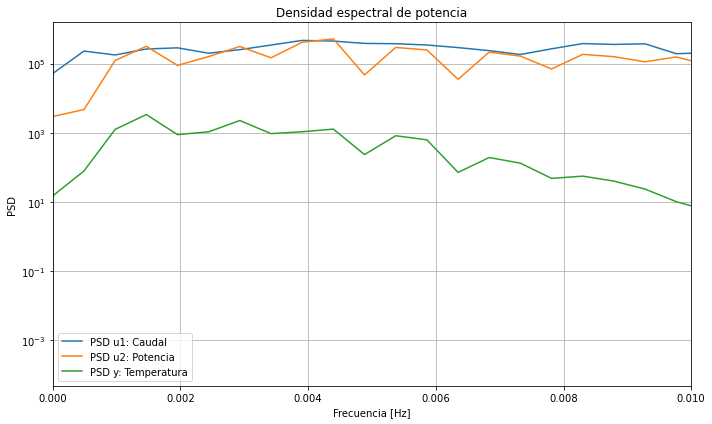
\includegraphics[width=\linewidth]{Figure 2026-06-22 153937 (1).png}
        \caption{Densidad espectral.}
        \label{fig:PSDmiso1}
    \end{subfigure}
    \hfill
    \begin{subfigure}[b]{0.48\textwidth}
        \centering
        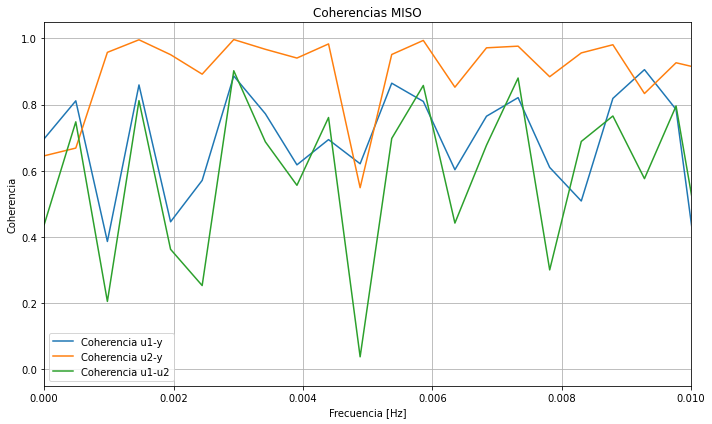
\includegraphics[width=\linewidth]{Figure 2026-06-22 153937 (2).png}
        \caption{Coherencias MISO (Naranja: potencia-temp; Azul: caudal-temp; Verde: caudal-potencia).}
        \label{fig:CoherenciasMISO}
    \end{subfigure}

    \vspace{0.5cm} % Espacio vertical entre filas

    % --- FILA 2 ---
    \begin{subfigure}[b]{0.48\textwidth}
        \centering
        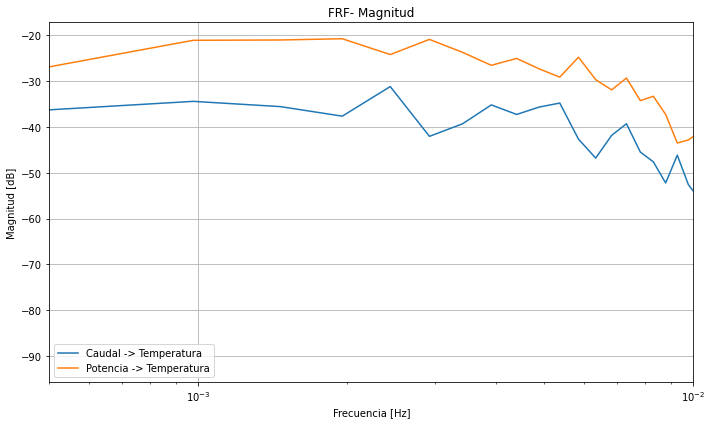
\includegraphics[width=\linewidth]{FRFmagnitud.png}
        \caption{FRF: Magnitud.} % <-- Ahora es la (c)
        \label{fig:magnitudFRFMISO}
    \end{subfigure}
    \hfill 
    \begin{subfigure}[b]{0.48\textwidth}
        \centering
        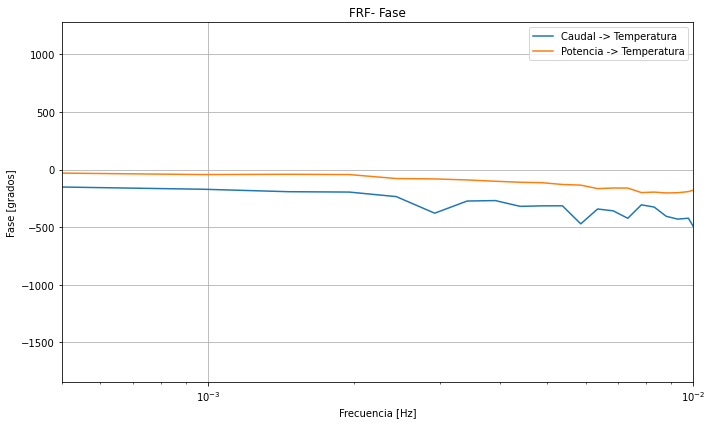
\includegraphics[width=\linewidth]{FRFfase.png}
        \caption{FRF: Fase.} % <-- Ahora es la (d)
        \label{fig:FASEfrfmiso}
    \end{subfigure}
    
    \vspace{0.5cm} % Espacio vertical antes de la última imagen

    % --- FILA 3 ---
    \begin{subfigure}[b]{0.48\textwidth}
        \centering
        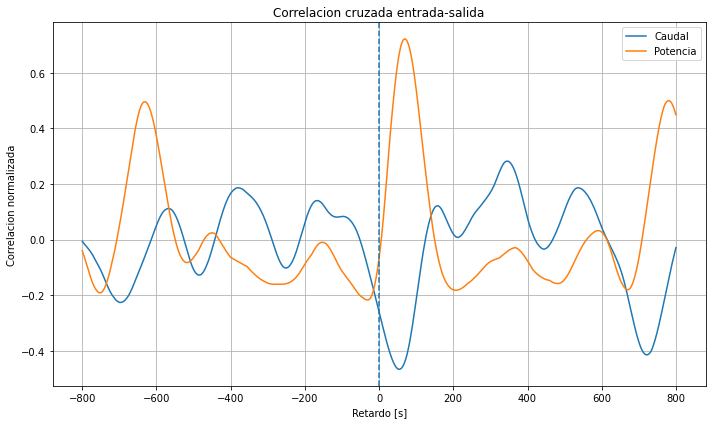
\includegraphics[width=\linewidth]{CorrelacionMISO.png}
        \caption{Correlación cruzada entre entradas.} % <-- Ahora es la (e)
        \label{fig:correlacionMISO}
    \end{subfigure}

    % --- CAPTION GLOBAL DE TODO EL GRUPO ---
    \caption{Análisis del primer conjunto de datos MISO: Densidad espectral, coherencias, respuesta en frecuencia y correlación cruzada.}
    \label{fig:analisis_MISO_completo}
\end{figure}

\subsubsection{Segundo experimento MISO}

El segundo experimento utilizó una variación en el caudal de 150 $L/h$ y la Figura \ref{fig:ResultadosMISO2doEXP} muestra los gráficos de los resultados obtenidos. 

Este segundo conjunto de datos presenta una adecuada concentración de energía en la banda de interés, con valores de 0.7665 para el caudal, 0.7492 para la potencia y 0.9170 para la temperatura. Además, la correlación temporal entre las entradas es baja, con un valor de −0.1509, lo que indica una baja dependencia lineal entre caudal y potencia. No obstante, la coherencia media entre caudal y temperatura resultó un valor medio de 0.5, observando en el gráfico (Figura \ref{fig:CoherenciaMISO2doEXP}) una curva baja, que evidencia una relación dinámica menos definida para este canal. La coherencia entre potencia y temperatura es una curva alta, cercana a la unidad, evidenciando que la potencia mantiene una influencia importante sobre la salida, aunque con un valor medio de 0.8, inferior a la observada en el anterior conjunto de datos.

La FRF estimada muestra que la potencia presenta una mayor magnitud que el caudal en prácticamente toda la banda de interés, evidenciando que la potencia eléctrica corresponde a la entrada dominante del sistema. Esta respuesta es coherente con el carácter térmico del banco experimental, ya que la potencia entrega energía directamente al fluido. La fase de la potencia presenta un comportamiento más regular en comparación con la fase del caudal, la cual es más variable, consistente con la menor coherencia observada para este canal. Así, la FRF indica que la potencia posee una influencia dinámica más claramente definida sobre la temperatura, mientras que el efecto del caudal es más débil y complejo.

La relación entre las señales de entrada se evaluó mediante el coeficiente correlación temporal entre el caudal y la potencia eléctrica, obteniendo un valor absoluto de 0.15. Este valor se encuentra por debajo del umbral de 0.8 utilizado como criterio de advertencia para dependencia entre canales de entrada \cite{csurcsia2020user}. También se calculó la correlación cruzada entre cada entrada y la temperatura de  salida. La potencia eléctrica presentó un máximo positivo en un retardo positivo, indicando que sus variaciones anteceden al incremento de temperatura. Esto es físicamente coherente, ya que la potencia constituye la fuente directa de energía térmica del sistema. En cambio, la correlación cruzada entre caudal y temperatura presentó un comportamiento de menor magnitud, lo que sugiere una relación dinámica más compleja e indirecta. Los valores negativos observados en la Figura \ref{fig:correlacionMISO2doEXP} para ciertos retardos positivos son consistentes con el efecto del caudal sobre el tiempo de residencia del fluido, dado que un aumento del flujo puede reducir el incremento térmico medido en la salida. En conjunto, el análisis confirma que ambas entradas aportan información dinámica al sistema, aunque la influencia de la potencia sobre la temperatura se manifiesta de forma más clara que la del caudal.
\begin{figure}[H]
    \centering
    % Primera fila: PSD y Coherencia
    \begin{subfigure}[b]{0.48\linewidth}
        \centering
        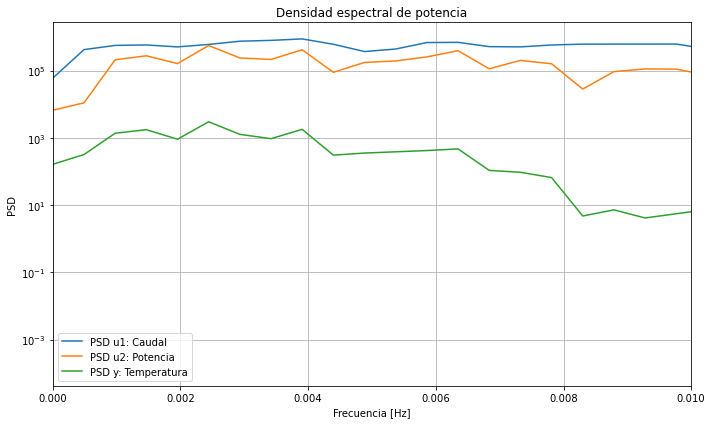
\includegraphics[width=\linewidth]{Figure 2026-06-24 211208 (1).png}
        \caption{Densidad espectral.}
        \label{fig:PSDmiso2doEXP}
    \end{subfigure}
    \hfill % Espacio horizontal entre imágenes
    \begin{subfigure}[b]{0.48\linewidth}
        \centering
        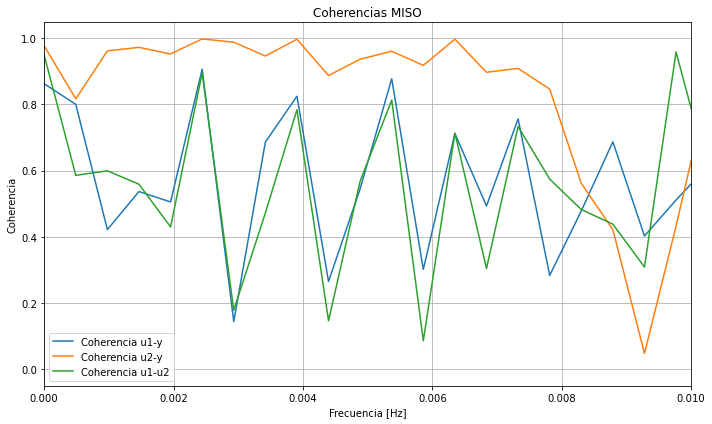
\includegraphics[width=\linewidth]{Figure 2026-06-24 211208 (2).png}
        \caption{Coherencias.}
        \label{fig:CoherenciaMISO2doEXP}
    \end{subfigure}

    \vspace{0.3cm} % Espacio vertical entre filas

    % Segunda fila: FRF Magnitud y Fase
    \begin{subfigure}[b]{0.48\linewidth}
        \centering
        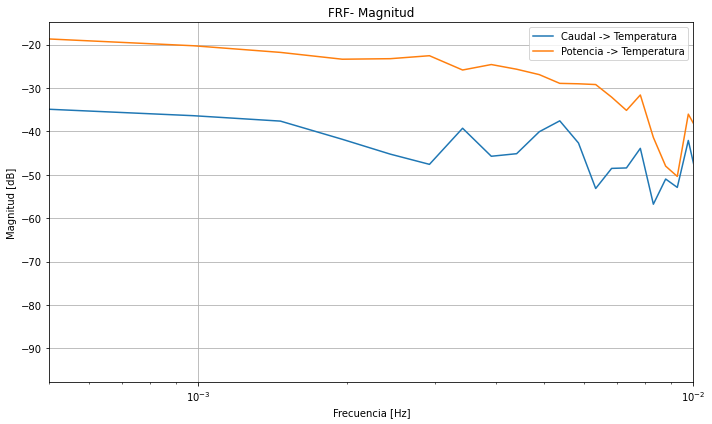
\includegraphics[width=\linewidth]{Figure 2026-06-24 211208 (4).png}
        \caption{FRF: Magnitud.}
        \label{fig:FRFmagnitudMISO2doEXP}
    \end{subfigure}
    \hfill
    \begin{subfigure}[b]{0.48\linewidth}
        \centering
        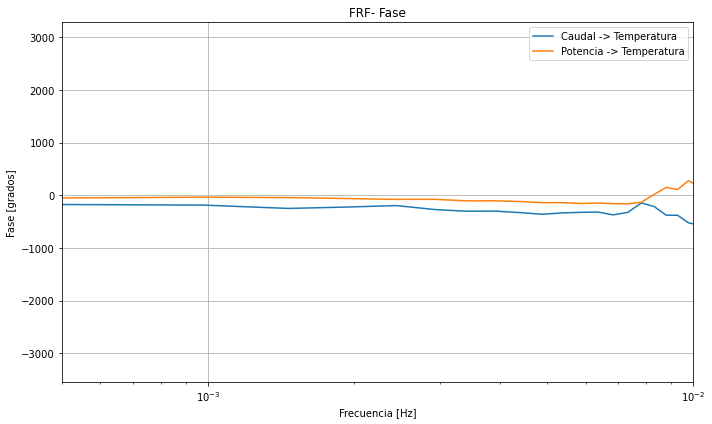
\includegraphics[width=\linewidth]{Figure 2026-06-24 211208 (5).png}
        \caption{FRF: Fase.}
        \label{fig:FRFfaseMISO2doExp}
    \end{subfigure}

    \vspace{0.3cm}

    % Tercera fila: Correlación (Centrada)
    \begin{subfigure}[b]{0.48\linewidth}
        \centering
        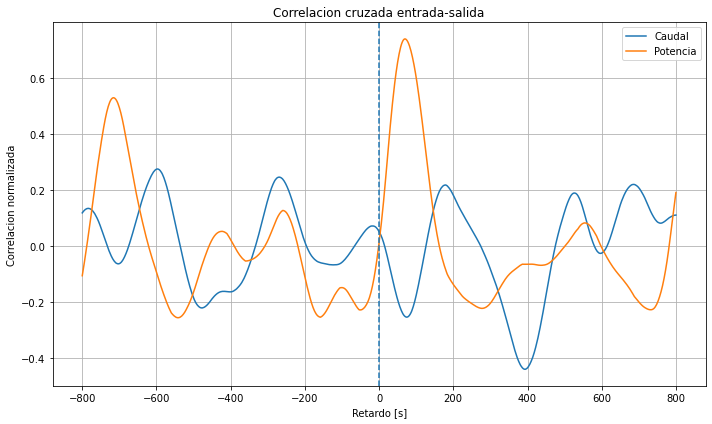
\includegraphics[width=\linewidth]{Figure 2026-06-24 211208 (8).png}
        \caption{Correlación cruzada entre entradas.}
        \label{fig:correlacionMISO2doEXP}
    \end{subfigure}

    % Captura y etiqueta global para todo el grupo
    \caption{Resultados del análisis MISO de la segunda prueba experimental.}
    \label{fig:ResultadosMISO2doEXP}
\end{figure}

\subsubsection{Tercer experimento MISO}
El tercer experimento MISO fue realizado con una variación en el caudal de 50 $L/h$.

El conjunto de datos analizado presenta una adecuada concentración de energía en la banda de interés, con valores de 0.6494 para el caudal, 0.7386 para la potencia y 0.8943 para la temperatura, observando también en la Figura \ref{fig:psdMISO3erEXP} que existe energía tanto en las entradas como en la salida. Estos resultados indican que las señales poseen contenido espectral suficiente dentro del rango de frecuencias considerado. Además, la correlación temporal entre las entradas fue de 0.05, valor absoluto considerablemente bajo, lo que evidencia una baja dependencia lineal entre caudal y potencia.

La coherencia media entre potencia y temperatura alcanzó un valor de 0.9549, lo que indica una relación dinámica fuerte y claramente definida entre la potencia eléctrica y la salida térmica. En contraste, la coherencia media entre caudal y temperatura fue de 0.5261, valor moderado que sugiere una influencia más débil e indirecta del caudal sobre la temperatura. El gráfico de coherencias (Figura \ref{fig:coherencis3erMISOEXP}) muestra la curva baja de la entrada del caudal. Este comportamiento también se observa en la FRF (Figuras \ref{fig:FRFmag3ERMISOexp} y \ref{fig:FRFfase3erMISOexp}), donde el canal potencia–temperatura presenta mayor magnitud y una fase más regular que el canal caudal–temperatura.

La correlación temporal entre las señales de entrada fue de -0.0583, valor muy cercano a cero y considerablemente inferior al umbral de 0.8 utilizado como criterio de advertencia para dependencia entre canales de entrada \cite{csurcsia2020user}. Este resultado indica que el caudal y la potencia eléctrica pueden considerarse prácticamente independientes desde el punto de vista temporal.

La correlación cruzada entre cada entrada y la temperatura de salida (Figura \ref{fig:correlacionMISO3erEXP}) muestra nuevamente que la potencia eléctrica presenta un máximo positivo claramente definido para retardos positivos, evidenciando que las variaciones de potencia anteceden al incremento de la temperatura. Este comportamiento es consistente con la naturaleza física del sistema, puesto que la potencia constituye la fuente directa de energía térmica. En contraste, la correlación entre caudal y temperatura presenta una magnitud considerablemente menor y un comportamiento más oscilatorio, sin un máximo dominante. Además, se observan valores negativos para determinados retardos positivos, lo que es coherente con el efecto del caudal sobre el tiempo de residencia del fluido, ya que un aumento del flujo puede reducir el incremento de temperatura en la salida. En conjunto, estos resultados confirman que ambas entradas aportan información dinámica al sistema, aunque la influencia de la potencia es más directa y claramente identificable, mientras que la del caudal es más compleja e indirecta.
\begin{figure}[H]
    \centering
    
    % Primera Fila
    \begin{subfigure}[b]{0.45\textwidth}
        \centering
        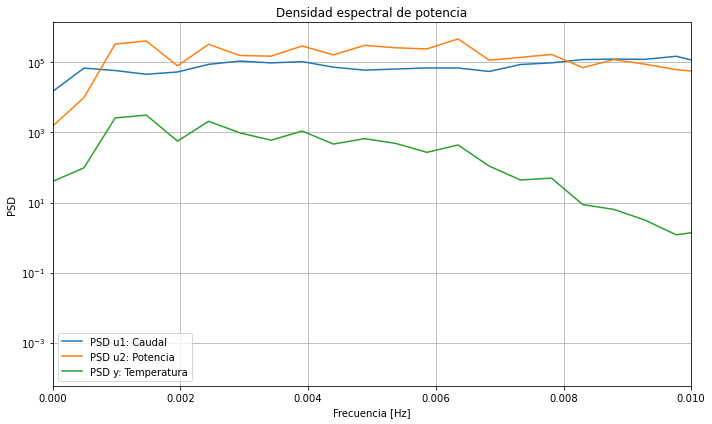
\includegraphics[width=\textwidth]{Figure 2026-06-25 131631 (1).png}
        \caption{Densidad espectral.}
        \label{fig:psdMISO3erEXP}
    \end{subfigure}
    \hfill % Espacio horizontal entre las dos imágenes
    \begin{subfigure}[b]{0.45\textwidth}
        \centering
        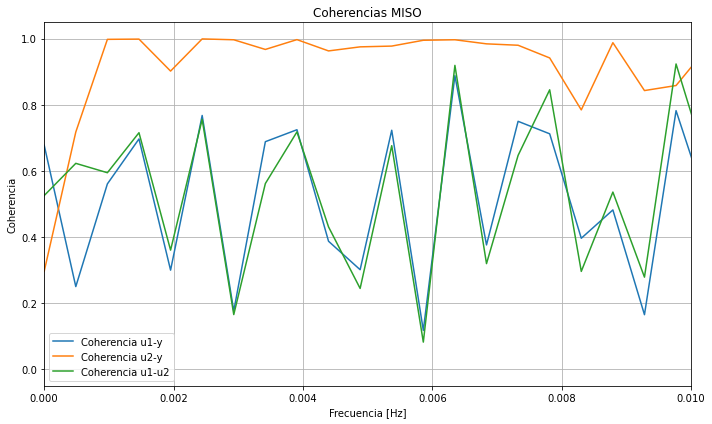
\includegraphics[width=\textwidth]{Figure 2026-06-25 131631 (2).png}
        \caption{Coherencia.}
        \label{fig:coherencis3erMISOEXP}
    \end{subfigure}
    
    \vspace{0.5cm} % Espacio vertical entre filas
    
    % Segunda Fila
    \begin{subfigure}[b]{0.45\textwidth}
        \centering
        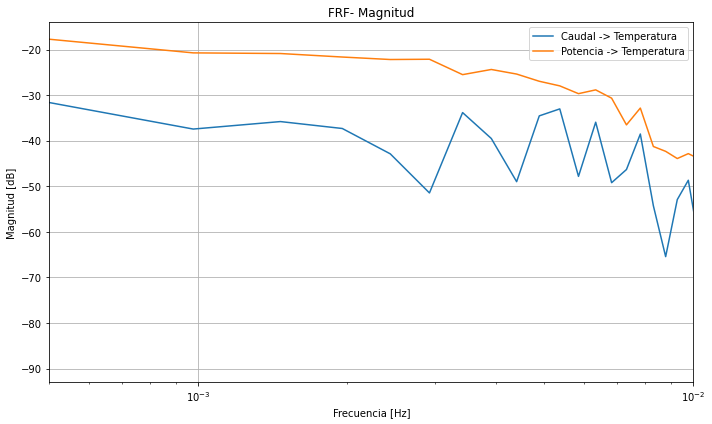
\includegraphics[width=\textwidth]{Figure 2026-06-25 131631 (4).png}
        \caption{FRF: Magnitud.}
        \label{fig:FRFmag3ERMISOexp}
    \end{subfigure}
    \hfill
    \begin{subfigure}[b]{0.45\textwidth}
        \centering
        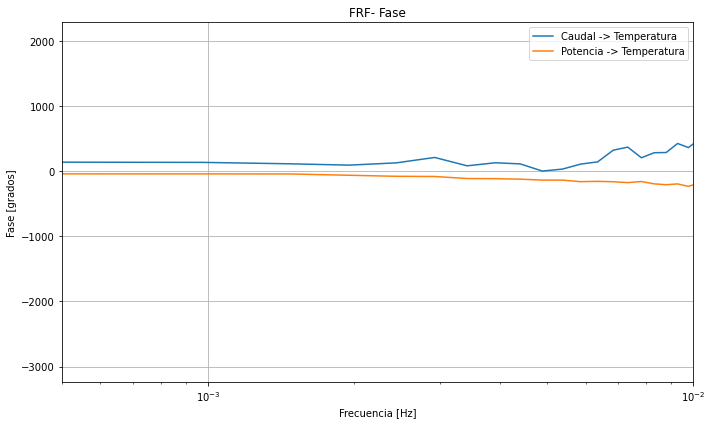
\includegraphics[width=\textwidth]{Figure 2026-06-25 131631 (5).png}
        \caption{FRF: Fase.}
        \label{fig:FRFfase3erMISOexp}
    \end{subfigure}
    
    \vspace{0.5cm}
    
    % Tercera Fila (Última imagen centrada)
    \begin{subfigure}[b]{0.45\textwidth}
        \centering
        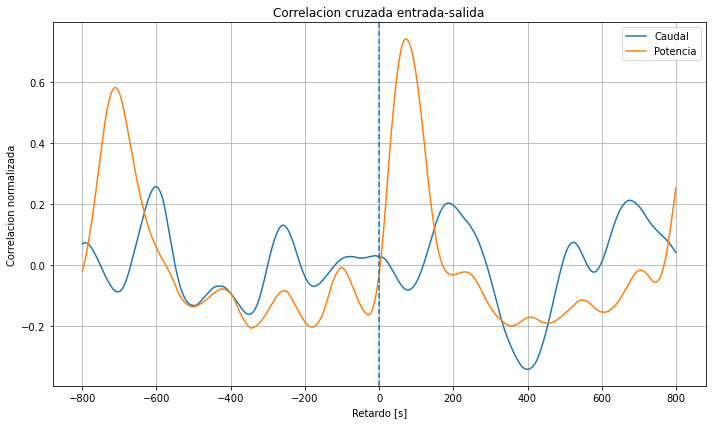
\includegraphics[width=\textwidth]{Figure 2026-06-25 131631 (8).png}
        \caption{Correlación cruzada.}
        \label{fig:correlacionMISO3erEXP}
    \end{subfigure}

    % Título global de todo el grupo de imágenes
    \caption{Análisis espectral y de respuesta en frecuencia para el tercer experimento MISO.}
    \label{fig:analisis_completo_MISO}
\end{figure}


\subsubsection{Cuarto experimento MISO}


El cuarto experimento MISO fue realizado utilizando señales PRBS tanto en el caudal como en la potencia eléctrica. A diferencia de los ensayos anteriores, en este caso ambas entradas fueron excitadas mediante señales pseudoaleatorias, lo que permite generar un conjunto de datos independiente y con características distintas para la validación posterior de los modelos.

El análisis espectral muestra que las señales presentan una concentración adecuada de energía dentro de la banda de interés. En particular, la energía del caudal en la banda fue de 0.5424, mientras que para la potencia alcanzó un valor de 0.7277. En el caso de la salida, la temperatura presentó una concentración de energía de 0.9071 dentro de la banda analizada, lo que se puede observar también la Figura \ref{fig:DensidadcuartoMISO}. Esto indica que, aunque el caudal presenta una menor energía relativa en comparación con los otros ensayos, la salida conserva una respuesta dominada por el rango frecuencial de interés del sistema térmico.

La coherencia media entre potencia y temperatura fue de 0.9612, la curva más alta observada en la Figura \ref{fig:coherenciacuartoMISO}, lo que confirma nuevamente que la potencia eléctrica mantiene una relación dinámica fuerte y claramente definida con la temperatura de salida. En cambio, la coherencia media entre caudal y temperatura fue de 0.5172, valor moderado que evidencia que el efecto del caudal sobre la temperatura sigue siendo más débil e indirecto. Este comportamiento es coherente con los ensayos anteriores, donde la potencia aparece como la entrada dominante del sistema, mientras que el caudal afecta la respuesta térmica de manera más compleja, asociada al transporte de energía y al tiempo de residencia del fluido.

La magnitud de la FRF (Figura \ref{fig:magnitudMISOCUARTOexp}) muestra nuevamente que el canal potencia–temperatura presenta una ganancia mayor que el canal caudal–temperatura en prácticamente toda la banda analizada. Esto confirma que la potencia eléctrica corresponde a la entrada con mayor influencia dinámica sobre la temperatura, debido a que representa el aporte directo de energía térmica al sistema. En cambio, la magnitud asociada al canal caudal–temperatura es menor y presenta un comportamiento más irregular, lo que indica que el efecto del caudal sobre la temperatura es más débil, indirecto y dependiente de la frecuencia. En la FRF de fase (Figura \ref{fig:faseFFRFcuartoexp}) se observa un comportamiento similar. La fase del canal potencia–temperatura presenta una tendencia más regular y con menor variación a lo largo de la banda de interés, lo que sugiere una relación dinámica más directa entre la potencia aplicada y la temperatura de salida. Por el contrario, la fase del canal caudal–temperatura es considerablemente más negativa y variable, lo que puede asociarse a un mayor retardo efectivo, a una dinámica de transporte más compleja y a la menor coherencia observada para este canal. Este resultado es físicamente consistente, ya que el caudal no entrega energía directamente al sistema, sino que modifica el tiempo de residencia del fluido y el transporte de calor a través del banco de ensayos.

Por otra parte, la correlación temporal entre las entradas fue de -0.0612, lo que indica una baja dependencia lineal entre el caudal y la potencia. Este valor es considerablemente menor al umbral de 0.8 utilizado como criterio de advertencia para dependencia entre entradas, por lo que ambas señales pueden considerarse suficientemente independientes desde el punto de vista temporal. 
En la correlación cruzada entrada-salida del cuarto experimento (Figura \ref{fig:correlacion4TOmisoEXP}) se observa nuevamente una diferencia clara entre el efecto de la potencia y el efecto del caudal sobre la temperatura. La señal de potencia presenta un máximo positivo bien definido para retardos positivos, con un valor cercano a 0.7. Esto indica que las variaciones de potencia anteceden a los cambios de temperatura, lo cual es físicamente coherente, ya que la potencia eléctrica representa el aporte directo de energía térmica al sistema. El hecho de que el máximo ocurra después de un cierto retardo confirma que la respuesta térmica no es inmediata, sino que está afectada por la inercia térmica del banco de ensayos y por el tiempo requerido para que el calor suministrado se refleje en la temperatura de salida. En cambio, la correlación cruzada entre caudal y temperatura presenta valores de menor magnitud y una forma más oscilatoria, sin un máximo positivo claramente dominante. Esto sugiere que el efecto del caudal sobre la temperatura es menos directo que el de la potencia.
\begin{figure}[H] 
    \centering

    % --- FILA 1 ---
    \begin{subfigure}[b]{0.48\textwidth}
        \centering
        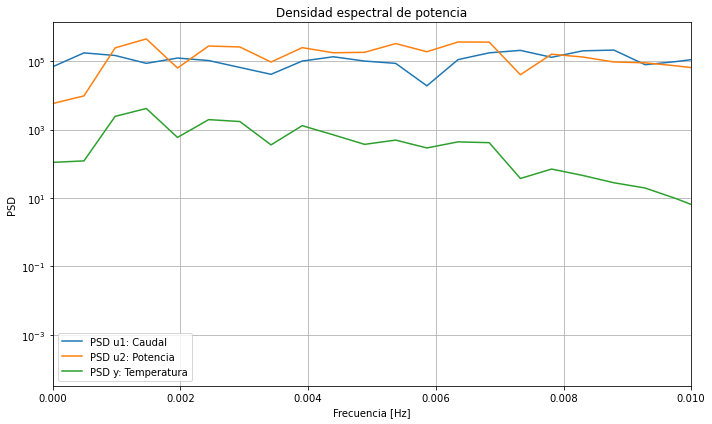
\includegraphics[width=\linewidth]{Figure 2026-07-07 161647 (1).png}
        \caption{Densidad espectral con ambas entradas con señal PRBS.}
        \label{fig:DensidadcuartoMISO}
    \end{subfigure}
    \hfill
    \begin{subfigure}[b]{0.48\textwidth}
        \centering
        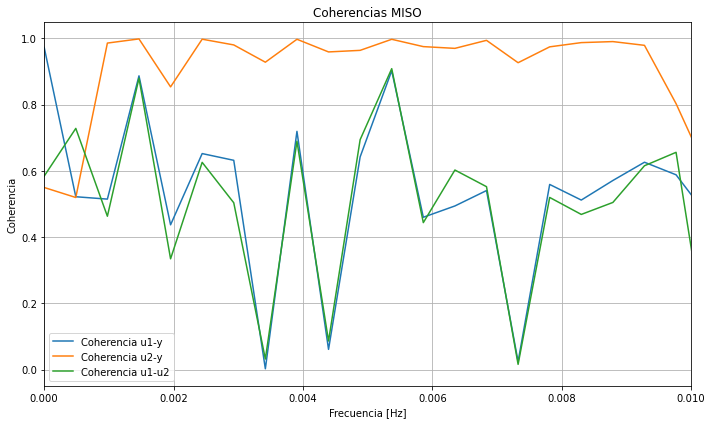
\includegraphics[width=\linewidth]{Figure 2026-07-07 161647 (2).png}
        \caption{Coherencia con ambas entradas con señal PRBS.}
        \label{fig:coherenciacuartoMISO}
    \end{subfigure}

    \vspace{0.5cm} % Espacio vertical entre filas

    % --- FILA 2 ---
    \begin{subfigure}[b]{0.48\textwidth}
        \centering
        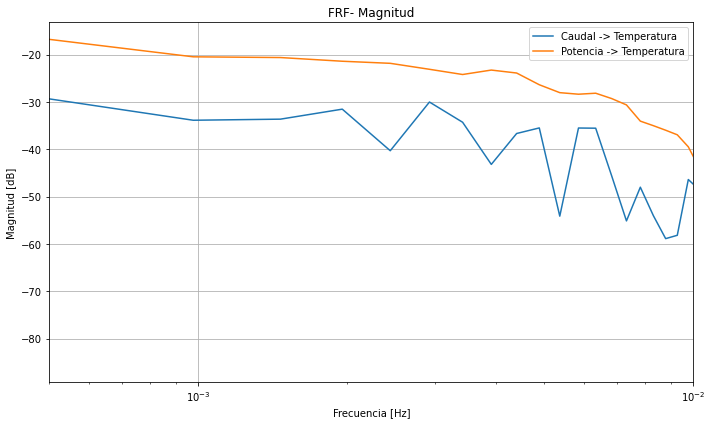
\includegraphics[width=\linewidth]{Figure 2026-07-07 161647 (4).png}
        \caption{FRF: Magnitud.}
        \label{fig:magnitudMISOCUARTOexp}
    \end{subfigure}
    \hfill
    \begin{subfigure}[b]{0.48\textwidth}
        \centering
        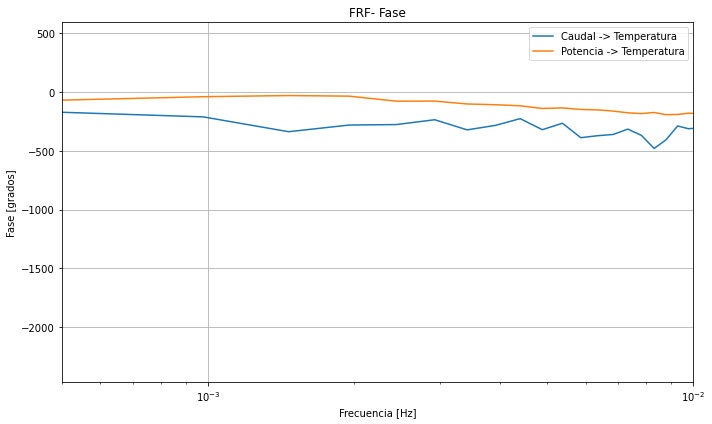
\includegraphics[width=\linewidth]{Figure 2026-07-07 161647 (5).png}
        \caption{FRF: Fase.}
        \label{fig:faseFFRFcuartoexp}
    \end{subfigure}

    \vspace{0.5cm} % Espacio vertical antes de la última imagen

    % --- FILA 3 (Imagen centrada) ---
    \begin{subfigure}[b]{0.5\textwidth}
        \centering
        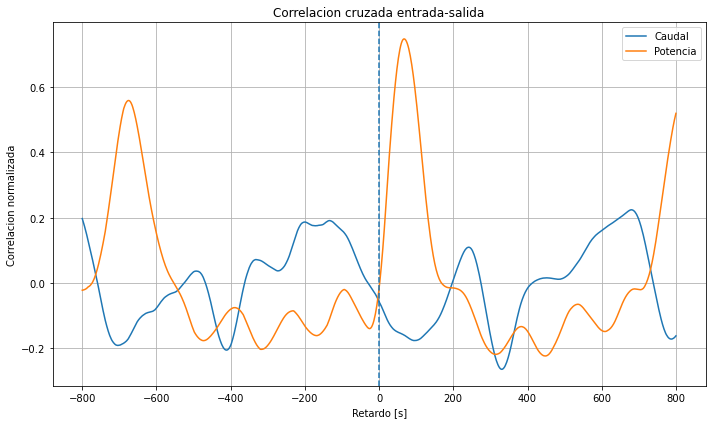
\includegraphics[width=\linewidth]{Figure 2026-07-07 161647 (8).png}
        \caption{Correlación.}
        \label{fig:correlacion4TOmisoEXP}
    \end{subfigure}

    % Título global para todo el grupo de imágenes
    \caption{Resultados del cuarto conjunto de datos obtenido empleando señales PRBS.}
    \label{fig:grupo_completo_experimento4}
\end{figure}

\subsubsection{Conclusiones de los experimentos}
Al comparar los cuatro conjuntos de datos MISO, se observa que todos presentan contenido espectral dentro de la banda de interés y aportan información útil para el análisis dinámico del sistema térmico. Sin embargo, existen diferencias importantes en la calidad de la relación entre entradas y salida, en la independencia entre las señales de entrada y en la claridad con que se manifiesta la dinámica de cada canal.

El primer conjunto de datos presenta el mejor equilibrio global para ser utilizado en la identificación de modelos MISO. Este ensayo posee una adecuada concentración de energía en la banda de interés, con valores de 0.7386 para el caudal, 0.7188 para la potencia y 0.9478 para la temperatura. Además, muestra una alta coherencia entre potencia y temperatura y una coherencia entre el caudal y la temperatura más alta que la observada en otros ensayos. Esto indica que ambas entradas aportan información relevante para representar la dinámica del sistema, siendo la potencia la entrada de mayor influencia directa y el caudal una entrada con efecto más indirecto, pero aún identificable. Otro aspecto relevante del primer conjunto es la baja correlación temporal entre las entradas, con un valor absoluto cercano a 0.22. Este valor se encuentra por debajo del umbral de 0.8 utilizado como criterio de advertencia, por lo que las señales de caudal y potencia pueden considerarse suficientemente independientes para la identificación. Esta condición es importante en modelos MISO, ya que una alta correlación entre entradas dificulta separar el efecto individual de cada una sobre la salida. Por lo tanto, el primer experimento entrega una combinación adecuada entre energía en banda, coherencia entrada–salida e independencia temporal entre entradas.

El segundo conjunto presenta una mayor energía relativa en las entradas, pero la relación dinámica entre caudal y temperatura es menos definida. La coherencia media entre caudal y temperatura es menor que en el primer ensayo, lo que puede dificultar la identificación precisa del efecto del caudal sobre la salida. Por su parte, el tercer conjunto presenta una baja correlación temporal entre entradas y una alta coherencia potencia–temperatura, pero nuevamente la entrada del caudal aparece con una influencia más débil. Esto sugiere que, aunque estos conjuntos son informativos, no entregan el mismo equilibrio que el primer ensayo para identificar simultáneamente la dinámica asociada a ambas entradas.

El cuarto conjunto de datos, generado con señales PRBS tanto en caudal como en potencia, presenta condiciones favorables para la validación. Su correlación temporal entre entradas es baja y mantiene una alta coherencia entre potencia y temperatura, con un valor medio de 0.9612. Además, la salida conserva una alta concentración de energía dentro de la banda de interés, con un valor de 0.9071. Aunque la coherencia entre caudal y temperatura es moderada, este comportamiento es consistente con los demás ensayos y confirma que el efecto del caudal sobre la temperatura es más débil y dependiente de la frecuencia.

A partir de este análisis, se define utilizar el primer conjunto de datos para la identificación de los modelos MISO. Esta elección se justifica porque dicho conjunto presenta el mejor compromiso entre excitación en la banda de interés, coherencia entrada–salida e independencia temporal entre entradas. En particular, permite identificar la influencia dominante de la potencia eléctrica sobre la temperatura, sin descartar el efecto dinámico del caudal, el cual también presenta información relevante dentro del rango frecuencial analizado.

Por otra parte, el cuarto conjunto de datos será utilizado para la validación en simulación libre. Esta decisión se justifica porque corresponde a un ensayo independiente, generado con señales PRBS en ambas entradas, lo que entrega una condición de evaluación distinta a la utilizada en la identificación. De esta manera, la validación no solo permite medir el ajuste del modelo frente a nuevos datos, sino también evaluar su capacidad de generalización ante variaciones simultáneas del caudal y la potencia eléctrica.

En conjunto, el análisis de los ensayos MISO confirma que el sistema térmico está dominado principalmente por la potencia eléctrica, ya que en todos los casos la coherencia entre potencia y temperatura fue mayor que la coherencia caudal y temperatura. Esto debido a la naturaleza física del banco de ensayos, donde la potencia entrega energía directamente al sistema, mientras que el caudal modifica el transporte térmico y el tiempo de residencia del fluido. El efecto del caudal, por lo tanto, aparece como una dinámica más débil, variable y dependiente de la frecuencia.

Las diferencias observadas entre los ensayos, especialmente en las coherencias entrada y salida y en la forma de las FRF, también sugieren que la respuesta del sistema no se mantiene completamente invariante frente a distintas condiciones de excitación. Este comportamiento puede estar asociado a efectos no lineales, variaciones del punto de operación o interacciones entre las entradas. En particular, desde el punto de vista físico, el incremento de temperatura depende de la relación entre la potencia térmica suministrada y el caudal del fluido, por lo que el efecto de una entrada puede depender del nivel de la otra.

Por esta razón, el primer conjunto se utilizará para la identificación de modelos MISO, mientras que el cuarto conjunto será reservado para la validación en simulación libre. Esta estrategia permite identificar los modelos con un conjunto que presenta buena calidad informativa y validarlos con un registro independiente y exigente. Además, los resultados obtenidos justifican no solo la evaluación de modelos MISO lineales, sino también de estructuras MISO no lineales, capaces de representar posibles interacciones entre caudal, potencia y temperatura.






\begin{comment}
    

Al comparar los tres conjuntos de datos experimentales, se observa que todos presentan condiciones adecuadas para la identificación, aunque con diferencias relevantes en la relación entre entradas y salida. El primer conjunto presenta el mejor equilibrio global, ya que posee una adecuada concentración de energía en la banda de interés y las mayores coherencias entre entrada y salida, especialmente en el canal de canal y temperatura. El segundo conjunto presenta la mayor energía de excitación en las entradas, aunque con coherencias entre entradas y  salidas menores a las observadas en el primer conjunto. El tercer conjunto muestra la menor correlación temporal entre entradas y la mayor coherencia entre potencia y temperatura, pero el efecto del caudal sobre la salida aparece menos definido.

Así, el análisis comparativo de los tres conjuntos de datos muestra que el sistema presenta una dinámica MISO dominada por la potencia eléctrica. En todos los casos, la coherencia entre potencia y temperatura fue superior a la coherencia entre caudal y temperatura, lo que evidencia que la potencia constituye la entrada con mayor influencia directa sobre la respuesta térmica. En cambio, el efecto del caudal aparece más débil y variable entre experimentos, lo que sugiere una dinámica más compleja asociada al transporte térmico y al tiempo de residencia del fluido.

Las diferencias observadas entre los conjuntos de datos, especialmente en las coherencias entrada–salida y en la forma de las FRF, indican que la respuesta del sistema no se mantiene completamente invariante frente a distintas condiciones de excitación. Este comportamiento es compatible con la presencia de efectos no lineales o dependientes del punto de operación. En particular, desde el punto de vista físico, el incremento de temperatura depende de la relación entre potencia térmica y caudal másico, por lo que el efecto de la potencia puede variar con el caudal.
\end{comment}

\section{Identificación de modelos MISO}

Según el análisis desarrollado en la sección anterior, en la que se evaluaron distintas estructuras lineales SISO, el modelo Box-Jenkins presentó el mejor desempeño en simulación libre. A partir de este resultado, la presente sección comienza con la identificación de un nuevo modelo Box-Jenkins lineal con dos entradas y una salida correspondiente a la temperatura del sistema. Posteriormente, se evalúa una estructura NARX, definida como una extensión no lineal del modelo ARX, capaz de representar relaciones no lineales entre las entradas, las salidas pasadas y la respuesta térmica del sistema. Se finaliza con la identificación y validación de un modelo de red neuronal que utiliza ecuaciones diferenciales ordinarias para calcular la salida.


Para la identificación de los modelos MISO, la variable de salida se expresó como una variación de temperatura respecto de una condición de referencia, de la misma forma que se obtuvieron los últimos tres modelos lineales. Esta temperatura de referencia correspondió al valor registrado a los 500 segundos en el conjunto de datos de identificación, instante en el que finaliza el periodo inicial de estabilización del sistema.
%De este modo, la salida utilizada para identificar los modelos se definió como:

%$$\Delta T(k)=T(k)-T_{base}$$
%Donde $T_{base}$ corresponde a la temperatura del sistema en t=500 segundos del experimento de identificación.
Durante la simulación libre, los modelos estimaron exclusivamente la evolución de $\Delta T$ a partir de las entradas, sin utilizar la temperatura experimental del conjunto de validación. Posteriormente, la temperatura absoluta simulada es reconstruida mediante:
$$\hat{T}(k)=T_{base}+\hat{\Delta T}(k)$$
Donde $\hat{T}(k)$ es la temperatura absoluta simulada, $T_{base}$ corresponde a la temperatura del sistema en t=500 segundos del experimento de identificación y $\hat{\Delta T}(k)$ es la diferencia de temperatura entregada por el modelo.

Se mantuvo la misma temperatura base utilizada durante la identificación porque el modelo fue ajustado para representar variaciones térmicas respecto de ese punto de operación. Cambiar esta referencia por la temperatura ambiente del conjunto de validación introduciría un desplazamiento distinto al empleado durante el entrenamiento, modificando artificialmente el nivel de la salida simulada y dificultando la evaluación de la dinámica identificada. Además, utilizar una temperatura obtenida específicamente del conjunto de validación podría incorporar información particular de dicho experimento en la reconstrucción de la salida, reduciendo la independencia de la simulación libre.

Este criterio difiere del utilizado previamente en los modelos SISO, en los que la temperatura ambiente del conjunto de validación se empleó como referencia para reconstruir la temperatura absoluta. En el análisis MISO se privilegió la consistencia entre la variable utilizada durante la identificación y la empleada durante la validación, manteniendo un mismo punto de referencia para todos los modelos comparados. No obstante, este procedimiento supone que ambos experimentos presentan condiciones térmicas iniciales comparables; por ello, las diferencias persistentes de nivel entre la salida real y simulada deben interpretarse también considerando posibles variaciones en las condiciones iniciales de operación.

\subsection{Modelo Box-Jenkins MISO}
El código SISO descrito anteriormente y el código MISO usado ahora siguen la misma metodología general de identificación del modelo, pero presentan diferencias necesarias debido a la cantidad de entradas consideradas en cada caso. El código SISO identifica un modelo con una sola entrada, correspondiente al caudal, mientras que el código MISO identifica un modelo con dos entradas, correspondientes al caudal y la potencia. Por esta razón, ambos códigos son equivalentes en su lógica de búsqueda y estimación, mas no en la estructura del modelo ni en la cantidad de parámetros que deben ser identificados.

%La estructura del modelo SISO se expresa mediante una única función de trasferencia entre la entrada y la salida: 
%$$y(k)=\frac{B(q)}{F(q)}u(k)+\frac{C(q)}{D(q)}e(k)$$

%En este caso, el modelo identifica solo un numerador $B$, un denominador $F$ para la dinámica entre la entrada y la salida y un modelo de ruido definido por lo polinomios $C$ y $D$. Esta estructura es adecuada cuando se desea representar la influencia de una sola variable de entrada sobre la salida del sistema.

Para el código MISO se  conserva la misma lógica de la función de transferencia del modelo (Ecuación \ref{ecuacionBJ}), pero se extiende su parte determinística para incorporar dos entradas. En este caso, la salida se modela como la suma de dos contribuciones independientes: una asociada al caudal y otra asociada a la potencia. La estructura general del modelo MISO queda dada por:

$$y(k)=\frac{B_1(q)}{F_1(q)}u_1(k)+\frac{B_2(q)}{F_2(q)}u_2(k)+\frac{C(q)}{D(q)}e(k)$$


La extensión a dos entradas implica que el procedimiento de identificación debe determinar un mayor número de órdenes estructurales. Para el canal caudal–temperatura se evaluaron distintas combinaciones de $n_{b1}$, $n_{f1}$ y $n_{k1}$, mientras que para el canal potencia-temperatura se exploraron los correspondientes $n_{b2}$, $n_{f2}$ y $n_{k2}$. Simultáneamente, se consideraron diferentes valores de $n_c$ y $n_d$ para el modelo del error. Al igual que en el caso SISO, estos órdenes no fueron establecidos previamente, sino seleccionados mediante el procedimiento de búsqueda y optimización, comparando las distintas estructuras candidatas de acuerdo con los criterios definidos para el modelo BJ. 

La inicialización de los parámetros siguió igualmente la estrategia utilizada en el modelo SISO, pero adaptada a la presencia de dos entradas. Para cada estructura candidata se construyó una aproximación inicial que incorporó valores pasados de la salida, del caudal y de la potencia, considerando además los retardos correspondientes a cada entrada. A partir de esta aproximación se obtuvieron valores iniciales para los coeficientes de $B_1(q)$, $F_1(q)$, $B_2(q)$ y $F_2(q)$, los cuales fueron posteriormente ajustados junto con $C(q)$ y $D(q)$ mediante el procedimiento iterativo de optimización. Por lo tanto, la diferencia respecto del caso SISO radica principalmente en que la búsqueda debe representar de forma simultánea dos relaciones dinámicas entrada-salida.

Como resultado del proceso de identificación y selección se obtuvo la siguiente estructura para el canal asociado al caudal: $n_{b1}=2$, $n_{f1}=2$ y $n_{k1}=30$.

El valor de $n_{b1}=2$ indica que el polinomio $B_1(q)$ contiene dos coeficientes asociados a la entrada de caudal. Si este valor fuera mayor, el modelo incorporaría una mayor cantidad de términos retardados de la entrada, aumentando su flexibilidad para representar la influencia del caudal, pero también su complejidad y el riesgo de sobreajuste. Por su parte, $n_{f1}=2$ establece una dinámica de segundo orden en el denominador $F_1(q)$. Un orden mayor permitiría representar comportamientos dinámicos más complejos, mientras que un orden menor daría lugar a una estructura más simple, aunque potencialmente insuficiente para reproducir la respuesta observada. Finalmente, $n_{k1}=30$ corresponde a un retardo discreto de 60 segundos para $T_s$=2 segundos. Un valor menor implicaría que el modelo considera una influencia más temprana del caudal sobre la temperatura, mientras que un valor mayor desplazaría dicha influencia hacia instantes posteriores. En este caso, los valores seleccionados corresponden a la combinación que presentó el mejor desempeño dentro de las estructuras evaluadas.



Para el canal asociado a la potencian se obtuvieron $n_{b2}=1$, $n_{f2}=2$ y $n_{k2}=33$. El valor de $n_{b2}=1$ indica que un único coeficiente en $B_2(q)$ fue suficiente para representar la influencia de la potencia dentro de la estructura seleccionada. Si se hubieran requerido valores mayores, esto habría indicado la necesidad de considerar una mayor cantidad de términos retardados de esta entrada. El orden $n_{f2}=2$ representa nuevamente una dinámica de segundo orden, mientras que $n_{k2}=33$ corresponde a un retardo modelado de 66 segundos. La diferencia entre $n_{k1}$ y $n_{k2}$ muestra que el procedimiento permitió asignar retardos distintos a cada canal, en lugar de imponer una misma respuesta temporal para ambas entradas.

La parte asociada al error fue definida mediante $n_c=2$ y $n_d=2$. Estos valores establecen una estructura de segundo orden para los polinomios $C(q)$ y $D(q)$, permitiendo representar dependencia temporal en la componente del error. Si estos órdenes fueran menores, la descripción de dicha dinámica sería más simple; si fueran mayores, el modelo dispondría de mayor flexibilidad para representar estructuras residuales más complejas, aunque a costa de aumentar el número de parámetros. La combinación seleccionada corresponde, por tanto, al equilibrio obtenido entre capacidad de representación del error y complejidad estructural.


A partir de los órdenes seleccionados se obtuvieron los siguientes polinomios para el canal caudal–temperatura:
$$B_1(q)=−0.00428057q^{-1}+0.00427947q^{−2}$$
$$F_1(q)=1−1.99205313q^{−1}+0.99690308q^{−2}$$
y para el canal potencia y temperatura:
$$B_2(q)=−0.00027389q^{−1}$$
$$F_2(q)=1−1.99820098q^{−1}+0.99834917q^{−2}$$

 La parte asociada al error quedó representada por:

$$C(q)=1−0.84738725q^{−1}+0.03734467q^{−2}$$
$$D(q)=1−1.96557062q^{−1}+0.96768592q^{-2}$$



Por lo tanto, la respuesta modelada se obtiene mediante la combinación de las contribuciones correspondientes al caudal y a la potencia, cada una caracterizada por su propia dinámica y retardo, mientras que $C(q)/D(q)$ representa la estructura temporal del error. La selección independiente de los órdenes de cada canal constituye una característica relevante de la formulación MISO, ya que permite representar diferencias en la forma y en el tiempo con que cada entrada se relaciona con la temperatura de salida.









\subsubsection{Simulación libre}

La simulación libre fue realizada para evaluar el desempeño de este modelo lineal Box-Jenkins MISO al someterlo a variaciones de caudal y potencia en las resistencias eléctricas. Este, al igual que el anterior SISO, fue identificado con una variación de temperatura o $\Delta T$, por lo que fue necesario un valor de temperatura base, que pueda elevar la salida del modelo a la salida real de temperatura. %Se utilizó, de la misma manera que con el sistema SISO, la temperatura ambiente que se tenia al momento de la toma de datos de la validación.

Los indicadores temporales fueron los siguientes:
\begin{itemize}
    \item RMSE      = 4.109 °C
\item MAE       = 3.261 °C
\item $R^2$     = -1.173
\item FIT       = -47.410 \%
\end{itemize}
\begin{comment}
    

\begin{itemize}
    \item RMSE      = 6.343 °C
\item MAE       = 5.398 °C
\item $R^2$     = -4.176
\item FIT       = -127.53 \%
\end{itemize}
\end{comment}
Los valores elevados de RMSE y MAE evidencian una diferencia entre las temperaturas real y simulada. En promedio, el error absoluto supera los 3 °C, lo que resulta elevado respecto del rango de variación térmica observado en el experimento. El valor negativo de $R^2$ indica que el modelo presenta un desempeño inferior al que se obtendría utilizando simplemente el valor medio de la temperatura experimental como estimación constante. De manera consistente, el FIT negativo evidencia que la trayectoria simulada no reproduce adecuadamente la evolución temporal de la salida real. En consecuencia, los indicadores temporales muestran que la estructura Box-Jenkins identificada no posee una capacidad predictiva satisfactoria en simulación libre.
En la comparación entre la temperatura real y la temperatura simulada (Figura \ref{fig:SIMLIBREbjMISO}) se observa que el modelo reproduce parcialmente el carácter oscilatorio del sistema, pero no logra representar correctamente la amplitud, el nivel medio ni la evolución temporal de la temperatura. Durante gran parte del experimento, la temperatura simulada se encuentra considerablemente por debajo de la temperatura real. Además, algunos máximos y mínimos aparecen desplazados temporalmente o presentan amplitudes muy diferentes de las observadas en el sistema real.
\begin{figure}[H]
    \centering
    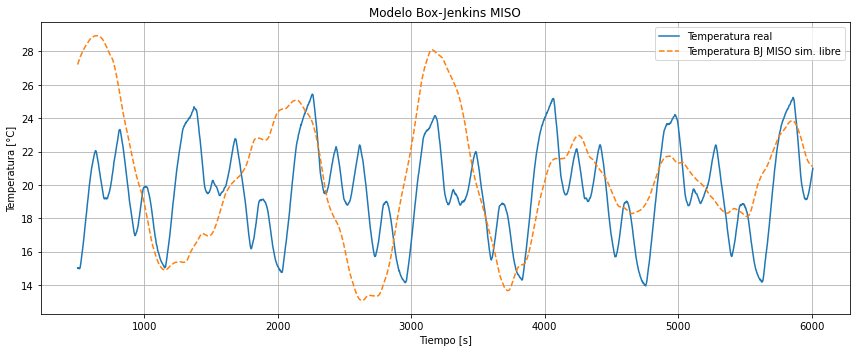
\includegraphics[width=0.5\linewidth]{Figure 2026-07-07 183108 (0).png}
    \caption{Gráfico de simulación libre del modelo BJ.}
    \label{fig:SIMLIBREbjMISO}
\end{figure}

En gráfico de residuos (Figura \ref{fig:ResiduosbjMISO}) se observan valores comprendidos aproximadamente entre −10 °C y 10 °C. Los errores más elevados se presentan aproximadamente entre 1200 y 1600 segundos y nuevamente alrededor de 2500 segundos, donde los residuos alcanzan sus valores máximos según la curva, cercanos a 10 °C. Además, estos no se distribuyen aleatoriamente alrededor de cero, sino que presentan oscilaciones persistentes y tendencias. La existencia de patrones estructurados en los residuos indica que estos conservan información determinística del proceso. Por lo tanto, el error no puede considerarse ruido blanco, y el modelo no logra capturar completamente las dinámicas asociadas a la acumulación y disipación de energía térmica.

La correlación entre el caudal y los residuos (Figura \ref{fig:correlacioncaudalresiduoBJMISO}) presenta valores de menor magnitud que los obtenidos para la potencia. La correlación caudal–residuo se mantiene aproximadamente entre −0.10 y 0.09, mostrando una estructura suave y persistente en distintos retardos. Aunque la magnitud de esta correlación es relativamente moderada, su comportamiento organizado y diferente de cero indica que parte del efecto del caudal permanece presente en el residuo. Esto sugiere que la contribución dinámica de esta entrada no ha sido completamente representada por el modelo.

En la correlación entre la potencia y los residuos (Figura \ref{fig:correlacionPOTENCIAresiduioBJMISO})  se observa un máximo positivo cercano a 0.31 para un retardo aproximado de 60 a 70 segundos, además de un mínimo cercano a −0.24 para retardos negativos próximos a −20 segundos. Esta estructura indica que el residuo conserva una relación significativa con la potencia eléctrica. Dado que la potencia fue identificada previamente como la entrada dominante del sistema, la presencia de correlación importante entre potencia y residuo sugiere que el modelo no capturó adecuadamente la dinámica principal de transferencia de energía hacia la temperatura de salida. 

En el análisis de densidad espectral de potencia (Figura \ref{fig:PSDBJmiso}) se observa que la PSD del modelo disminuye de forma importante a medida que aumenta la frecuencia. En bajas frecuencias, el modelo presenta cierto contenido energético, pero su energía cae rápidamente y queda por debajo de la PSD de la temperatura real en gran parte de la banda analizada. Por su parte, las entradas de caudal y potencia presentan alta energía en la banda de interés, lo que confirma que el problema no se debe a una falta de excitación de las señales de entrada. La diferencia entre la PSD real y la PSD simulada indica que el modelo no reproduce correctamente la distribución energética de la salida, especialmente en las componentes frecuenciales donde la temperatura real mantiene energía significativa.

La FRF de magnitud (Figura \ref{fig:FRFmagnitudBJMISO}) entrega una visión complementaria. En el canal caudal–temperatura, el modelo sigue parcialmente la tendencia decreciente de la FRF real, pero presenta diferencias importantes en distintos tramos de frecuencia. En la entrada del caudal, las diferencias son más marcadas, ya que la magnitud del modelo se separa de la magnitud real, especialmente desde frecuencias cercanas a 0.003 Hz en adelante. Esto indica que la ganancia dinámica estimada por el modelo no representa adecuadamente cómo las variaciones de potencia se transfieren hacia la temperatura. Considerando que la potencia es la entrada con mayor coherencia respecto de la salida, esta discrepancia es relevante y limita la capacidad predictiva del modelo.

El análisis de la fase (Figura \ref{fig:frfFASEBJMISO}) muestra diferencias importantes entre el sistema real y el modelo. Para la relación caudal–temperatura, las fases real y simulada presentan una separación considerable en gran parte de la banda. Para la relación potencia–temperatura también se observan discrepancias. Aunque ambas fases presentan una tendencia creciente en las frecuencias más bajas, la respuesta simulada alcanza valores superiores y exhibe una evolución diferente de la fase real. Estas diferencias indican que el modelo no reproduce correctamente los desfases ni los retardos dinámicos asociados a las entradas.




La coherencia entre las entradas y la temperatura real (Figura \ref{fig:coherenciaBJMISO}) presenta comportamientos diferentes para el caudal y la potencia. La relación potencia–temperatura real muestra una coherencia elevada en prácticamente toda la banda de frecuencias analizada. Este resultado confirma que la potencia constituye la entrada con mayor influencia sobre la respuesta térmica del sistema. Sin embargo, la coherencia potencia–temperatura simulada difiere considerablemente de la correspondiente al sistema real. Esta discrepancia indica que el modelo no reproduce correctamente la relación frecuencial entre la potencia y la temperatura. En el caso del caudal, la coherencia con la temperatura real es moderada y presenta variaciones importantes con la frecuencia. La coherencia asociada a la temperatura simulada tampoco coincide de manera consistente con la curva experimental. Las diferencias entre ambas curvas muestran que el modelo no representa adecuadamente la contribución del caudal en toda la banda de interés.



\begin{figure}[H] % Requiere \usepackage{float} en el preámbulo para fijar la posición
    \centering

    % --- FILA 1: Residuos y Densidad de Potencia ---
    \begin{subfigure}[b]{0.48\textwidth}
         \centering
    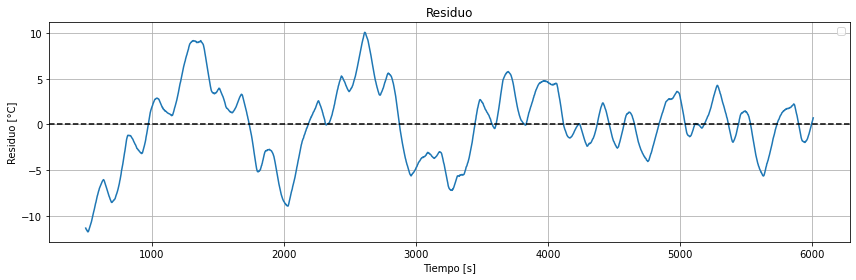
\includegraphics[width=\linewidth]{residosBJMISO.png}
    \caption{Residuos del modelo BJ.}
    \label{fig:ResiduosbjMISO}
    \end{subfigure}
    \hfill
    \begin{subfigure}[b]{0.48\textwidth}
        \centering
        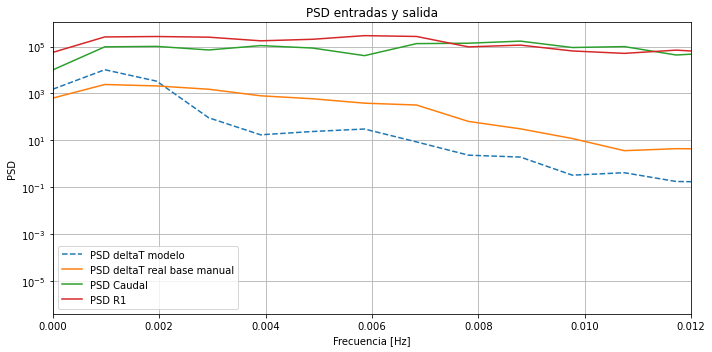
\includegraphics[width=\linewidth]{Figure 2026-07-07 183108 (7).png}
        \caption{Densidad de potencia.}
        \label{fig:PSDBJmiso}
    \end{subfigure}

    \vspace{0.4cm} % Espacio entre filas

    % --- FILA 2: Bloque de Correlaciones y Coherencia (Tres imágenes) ---
    \begin{subfigure}[b]{0.31\textwidth}
        \ \centering
    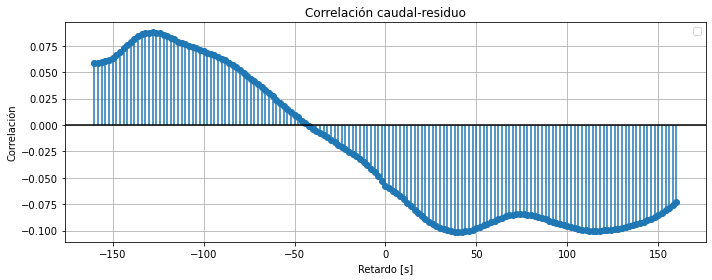
\includegraphics[width=\linewidth]{CORRELACIONnuevaCAUDAL-RESIDUO.png}
    \caption{Correlación caudal-residuos.}
    \label{fig:correlacioncaudalresiduoBJMISO}
    \end{subfigure}
    \hfill
    \begin{subfigure}[b]{0.31\textwidth}
       \centering
    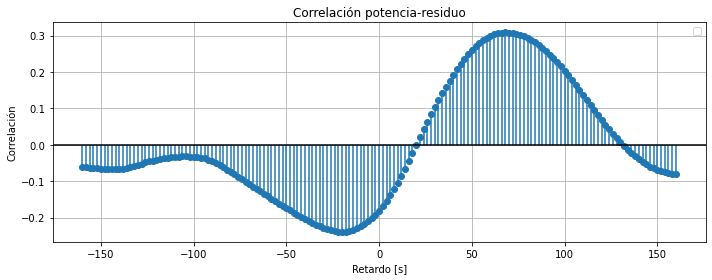
\includegraphics[width=\linewidth]{CORRELACIONnuevaPOTENCIA-RESIDUO.png}
    \caption{Correlación potencia-residuos.}
    \label{fig:correlacionPOTENCIAresiduioBJMISO}
    \end{subfigure}
    \hfill
    \begin{subfigure}[b]{0.31\textwidth}
       \centering
    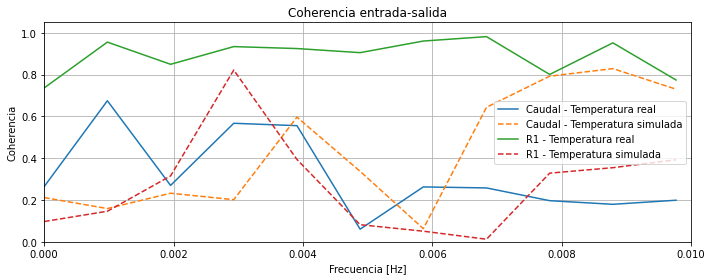
\includegraphics[width=\linewidth]{COHERENCIANUEVA.png}
    \caption{Coherencia.}
    \label{fig:coherenciaBJMISO}
    \end{subfigure}

    \vspace{0.4cm}

    % --- FILA 3: Respuesta en Frecuencia (FRF) ---
    \begin{subfigure}[b]{0.48\textwidth}
        \centering
        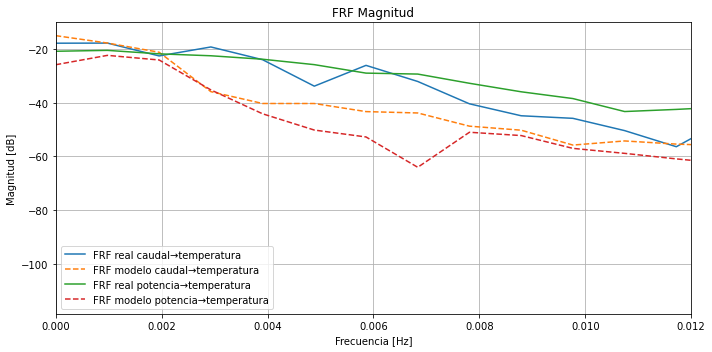
\includegraphics[width=\linewidth]{Figure 2026-07-07 183108 (8).png}
        \caption{FRF: Magnitud.}
        \label{fig:FRFmagnitudBJMISO}
    \end{subfigure}
    \hfill
    \begin{subfigure}[b]{0.48\textwidth}
         \centering
    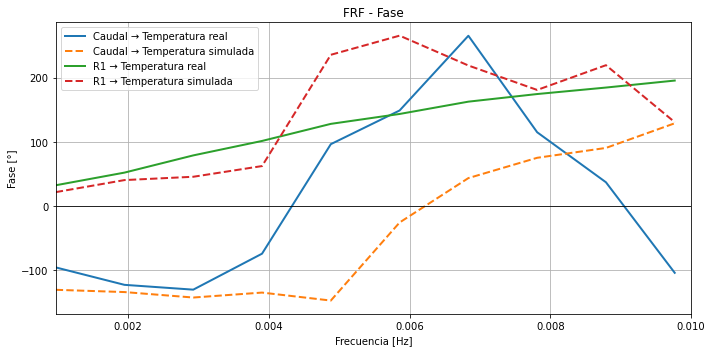
\includegraphics[width=\linewidth]{FASENUEVA.png}
    \caption{FRF: Fase.}
    \label{fig:frfFASEBJMISO}
    \end{subfigure}

    % Caption global para todo el conjunto
    \caption{Validación y análisis espectral del modelo Box-Jenkins MISO.}
    \label{fig:analisis_completo_BJ_MISO}
\end{figure}


En conjunto, los resultados muestran que el modelo Box-Jenkins MISO no logró mejorar la representación temporal del sistema en simulación libre. Aunque la estructura incorpora dos entradas y permite separar la dinámica determinística de la dinámica del error, los residuos presentan una estructura marcada, existe correlación significativa entre las entradas y el error, y las métricas temporales muestran un bajo desempeño. Además, la PSD y la FRF evidencian diferencias relevantes entre el modelo y el sistema real, especialmente en la representación del canal potencia–temperatura.

Este resultado sugiere que la dificultad no se debe únicamente a la cantidad de entradas consideradas, sino también a la capacidad de la estructura lineal para representar la dinámica real del sistema. El banco de ensayos térmico puede presentar interacciones no lineales entre potencia, caudal y temperatura, debido a que el incremento térmico no depende de manera independiente de cada entrada, sino de la relación entre el calor entregado y el flujo de agua que transporta esa energía. Además, las pérdidas térmicas, el tiempo de residencia del fluido, la acumulación de energía en los paneles y las variaciones del punto de operación pueden modificar la respuesta dinámica del sistema.

\subsection{Modelo NARX MISO}


A partir de las limitaciones observadas en los modelos lineales SISO y MISO, se evaluó una estructura no lineal NARX (Nonlinear AutoRegressive model with eXogenous inputs), utilizando como entradas el caudal y la potencia eléctrica, y como salida la variación de temperatura $\Delta T$. A diferencia de las estructuras lineales evaluadas previamente, el modelo NARX permite incorporar relaciones no lineales entre valores pasados de la salida y de las entradas, manteniendo al mismo tiempo una representación autorregresiva de la dinámica.

\begin{enumerate}
    \item \textbf{Preparación y división de los datos}


Al igual que en los modelos anteriores, se utilizaron únicamente los datos posteriores a los primeros 500 s, excluyendo el período inicial de estabilización. A partir de este instante se consideraron como variables el caudal, la potencia y la variación de temperatura. Posteriormente, los datos se dividieron cronológicamente, destinando el 80 \% inicial a la identificación y el 20 \% restante a la validación.
    \item \textbf{Definición de las estructuras NARX candidatas}

    Cada estructura se definió, según la Ecuación \ref{ecuacionNARX}, mediante los órdenes $n_a$, $n_{b1}$, $n_{b2}$, $n_{k1}$ y $n_{k2}$. El parámetro $n_{a}$ determina la cantidad de valores pasados de $\Delta T$ utilizados para estimar la salida actual. Los parámetros $n_{b1}$ y $n_{b2}$ establecen el número de valores retardados considerados para el caudal y la potencia, respectivamente, mientras que $n_{k1}$ y $n_{k2}$ determinan el primer retardo considerado para cada entrada. Estos valores no fueron fijados previamente. Se definieron rangos de búsqueda para cada uno de ellos y el código evaluó sistemáticamente las distintas combinaciones posibles.


    \item \textbf{Construcción de los regresores base}

    Para cada combinación candidata de órdenes se construyó un vector de regresores formado por valores pasados de la salida, del caudal y de la potencia. De manera general, este vector puede expresarse como:
$$\phi(k)=[y(k−1),...,y(k−n_a),u_1(k−n_{k1}),...,u_1(k−n_{k1}−n_{b1}+1), u_2(k−n_{k2}), ..., u_2(k−n_{k2}−n_{b2}+1)]$$

Cada fila de la matriz de regresores contiene, por tanto, la información histórica utilizada por el modelo para estimar $\Delta T$ en un instante determinado. El procedimiento se repite para cada combinación de órdenes incluida en la búsqueda.


\item \textbf{Normalización y expansión polinomial}

Una vez construidos los regresores, estos fueron normalizados utilizando la media y desviación estándar calculadas exclusivamente a partir del conjunto de identificación. Los mismos factores de normalización fueron posteriormente aplicados al conjunto de validación. La salida utilizada durante el ajuste también fue normalizada a partir de los datos de identificación. Este procedimiento permite evitar diferencias de escala entre variables como caudal, potencia y temperatura y mejorar el acondicionamiento numérico durante la estimación.

Posteriormente, los regresores normalizados fueron sometidos a una expansión polinomial de segundo grado. De esta manera, el modelo incorpora no solo los términos individuales de cada regresor, sino también sus cuadrados y productos cruzados. Así, por ejemplo, puede representar efectos asociados a $u_1^2$, $u_2^2$,$y(k-1)u_1(k-n_{k1})$ o $u_1(k-n_{k1})u_2(k-n_{k2})$. Esta expansión es la que introduce la capacidad no lineal del modelo. En esta identificación el grado polinomial se fijó previamente en 2, para mantener una complejidad computacional acotada.


\item \textbf{Estimación de los parámetros}

Una vez normalizados los regresores y realizada la expansión polinomial de segundo grado, se estimaron los coeficientes del modelo mediante regresión Ridge. Este método corresponde a una extensión de la regresión por mínimos cuadrados que, además de minimizar el error entre la salida medida y la estimada, incorpora una penalización sobre la magnitud de los coeficientes del modelo. Esta penalización es conveniente debido a que la expansión de segundo grado genera un número elevado de términos lineales, cuadráticos y de interacción, algunos de los cuales pueden presentar una fuerte dependencia entre sí. En estas condiciones, una estimación sin regularización puede generar coeficientes de gran magnitud y una elevada sensibilidad frente a pequeñas variaciones de los datos.

La regresión Ridge incorpora un parámetro de regularización $\alpha$, que controla el equilibrio entre el ajuste a los datos y la magnitud de los coeficientes estimados. Cuando $\alpha$ es muy pequeño, la penalización es débil y la solución se aproxima a la obtenida mediante mínimos cuadrados convencionales; en cambio, al aumentar $\alpha$, se penalizan con mayor intensidad los coeficientes elevados, obteniéndose una estructura menos sensible a los datos de identificación, aunque una regularización excesiva puede reducir la capacidad del modelo para representar la dinámica observada.

En este trabajo se utilizó $\alpha=10^{-4}$
, correspondiente a una regularización de baja intensidad. Este valor permite limitar la magnitud de los coeficientes y mejorar la estabilidad numérica sin afectar significativamente la capacidad de ajuste del modelo. Su selección se respaldó mediante un análisis de sensibilidad, en el cual se observó una reducción importante de la magnitud de los coeficientes sin variaciones apreciables en el RMSE ni en el FIT de validación. Además, $\alpha$ se mantuvo constante durante toda la exploración de órdenes y retardos, asegurando un mismo criterio de regularización para la comparación entre las distintas estructuras NARX.


\item \textbf{Evaluación de cada estructura candidata}

Una vez ajustado cada modelo, se calculó su respuesta sobre el conjunto de validación utilizando los regresores construidos con los datos reales disponibles. En esta etapa se evaluó, por tanto, el desempeño a un paso y se calcularon RMSE, MAE, FIT y $R^2$. También se contabilizó el número total de parámetros generado por la expansión polinomial.


\item \textbf{Selección de la estructura}

La selección de la estructura se realizó considerando un criterio que combina el error de validación, el porcentaje de ajuste y el número de parámetros, mediante una función de costo. De esta forma, se buscó un equilibrio entre precisión y complejidad, evitando seleccionar una estructura excesivamente grande que pudiera ajustarse al ruido de los datos en lugar de capturar la dinámica real del sistema.

    
\end{enumerate}





Como resultado del procedimiento de búsqueda, se obtuvo un modelo NARX MISO polinomial de segundo grado con los siguientes órdenes: $n_a=4$, $n_{b1}=3$, $n_{b2}=4$, $n_{k1}=4$, $n_{k2}=8$.

Estos valores corresponden a la combinación que presentó el menor valor de la función de costo entre las estructuras evaluadas. Por lo tanto, no fueron establecidos previamente a partir de supuestos físicos, sino seleccionados a partir del desempeño obtenido sobre los datos de validación y de la complejidad resultante del modelo.


El valor $n_a=4$ indica que la estimación de $\Delta T(k)$ utiliza las cuatro muestras anteriores de la salida: $y(k-1)$, $y(k-2)$, $y(k-3)$, $y(k-4)$

Con un período de muestreo de 2 segundos, esto significa que la estructura incorpora información de la evolución de la salida correspondiente a los 8 segundos anteriores. Si $n_a=4$ fuese mayor, el modelo dispondría de una historia más extensa de la salida, pero también aumentaría el número de regresores y, especialmente después de la expansión polinomial, la cantidad total de parámetros. Un valor menor produciría una estructura más simple, aunque podría resultar insuficiente para representar la dependencia temporal observada. La selección de $n_a=4$ indica que, dentro del rango explorado, este valor presentó el mejor compromiso según el criterio definido.


Para el caudal se obtuvieron $n_{b1}=3$ y $n_{k1}=4$. Esto significa que el modelo utiliza los regresores: $u_1(k-4)$, $u_1(k-5)$, $u_1(k-6)$

correspondientes a retardos de 8, 10 y 12 segundos (según $T_s=2$). valor $n_{k1}=4$ establece, por tanto, el primer instante retardado del caudal incorporado por la estructura, mientras que $n_{b1}=3$ determina cuántos términos consecutivos se utilizan a partir de ese retardo. Un valor mayor de $n_{b1}$  habría ampliado la ventana temporal de información del caudal, aumentando simultáneamente la complejidad del modelo.


Para la potencia el código seleccionó $n_{b2}=4$ y $n_{k2}=8$
Así, los regresores base utilizados fueron: $u_2(k−8), u_2(k−9), u_2(k−10), u_2(k−11)$.


que corresponden a retardos entre 16 y 22 segundos. De este modo, la estructura seleccionada comienza a incorporar información de la potencia en un instante posterior al considerado para el caudal. Esto indica que, dentro de la identificación realizada, un mayor retardo para la potencia produjo una mejor representación de los datos. Sin embargo, este valor debe interpretarse como un retardo identificado por el modelo y no necesariamente como una medición directa del tiempo físico de propagación térmica.


En conjunto, la estructura contiene 11 regresores base: $[y(k-1),y(k-2),y(k-3),y(k-4),u_1(k-4),u_1(k-5),u_1(k-6),u_2(k−8), u_2(k−9), u_2(k−10), u_2(k−11)]$.


A estos regresores se aplica posteriormente la expansión polinomial de segundo grado. Por lo tanto, el modelo no se limita a utilizar directamente los 11 términos anteriores, sino que incorpora también sus cuadrados e interacciones.

Esta estructura permite representar, por ejemplo, no solo el efecto individual del caudal o de la potencia, sino también posibles interacciones entre ambas entradas y entre estas y el estado térmico previo del sistema. Por esta razón, el incremento de complejidad respecto de las estructuras lineales no proviene únicamente de los retardos seleccionados, sino principalmente de la combinación no lineal de los regresores introducida mediante la expansión polinomial.

\subsubsection{Simulación libre}

La validación en simulación libre del modelo NARX muestra que logra reproducir adecuadamente la dinámica  real del sistema. En la comparación temporal (Figura \ref{fig:SimlibreNARX}) se observa que la temperatura simulada sigue una tendencia oscilatoria similar a la real, reproduciendo correctamente la sucesión de aumentos y disminuciones asociadas a las variaciones de las señales de entrada. No obstante, se observan diferencias principalmente en los máximos de temperatura, donde el modelo tiende a entregar amplitudes menores a las reales.
\begin{figure}[H]
    \centering
    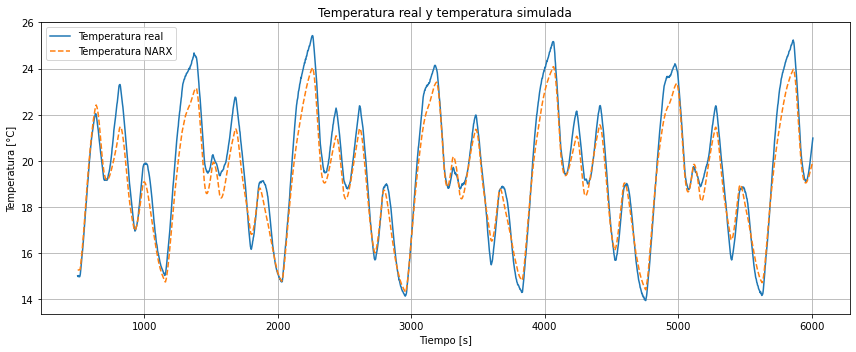
\includegraphics[width=0.5\linewidth]{GRAFICONARXconTbasenueva.png}
    \caption{Simulación libre del modelo NARX.}
    \label{fig:SimlibreNARX}
\end{figure}


Los indicadores temporales fueron:
\begin{itemize}
    \item RMSE: 0.756 °C
\item MAE: 0.614 °C
\item $R^2$: 0.927
\item FIT: 72.92\%
\end{itemize}
El RMSE y el MAE menores a 1 °C evidencian un error promedio bajo en la estimación de la temperatura. Además, el valor de $R^2$ indica una elevada concordancia con la variabilidad observada en la temperatura. De manera similar, el FIT  confirma que el modelo representa satisfactoriamente la evolución temporal del sistema durante la simulación libre. Sin embargo, este valor también indica que todavía existen componentes de la dinámica térmica que no son completamente reproducidos por la estructura NARX identificada. %Por lo tanto, a pesar de incorporar términos no lineales e interacciones entre caudal, potencia y temperatura pasada, la estructura identificada no presenta un desempeño satisfactorio en la validación temporal.
El gráfico de residuos (Figura \ref{fig:ResiduosNARX}) muestra que el error se mantiene mayoritariamente entre -1°C y 2°C. Además, estos no se distribuyen de forma completamente aleatoria alrededor de cero, sino que presentan oscilaciones persistentes y patrones que se repiten a lo largo del experimento. Esta estructura indica que el error conserva información dinámica que no ha sido totalmente capturada por el modelo. En particular, la mayor magnitud de los residuos en las proximidades de los máximos de temperatura sugiere que el NARX reproduce adecuadamente la tendencia y la periodicidad general del sistema, pero presenta limitaciones para representar con precisión la amplitud de algunas respuestas transitorias.

La correlación cruzada entre caudal y residuo (Figura \ref{fig:CorrelacionNARXCaudal}) evidencia que el error mantiene una relación estructurada con esta entrada. Se observan correlaciones positivas para retardos negativos y correlaciones negativas para retardos positivos, alcanzando valores cercanos a -0.2. Esto indica que parte del efecto dinámico del caudal permanece en el residuo. Desde el punto de vista de validación, este comportamiento muestra que el modelo no logró representar completamente la influencia del caudal sobre la temperatura. Además, la forma oscilatoria de la correlación es consistente con una dinámica de transporte térmico más compleja, donde el efecto del caudal no se manifiesta como una relación directa simple.

La correlación cruzada entre potencia y residuo (Figura \ref{fig:CorrelacionNARXpotencia}) presenta un máximo positivo cercano a 0.6 para retardos positivos, aproximadamente entre 70 y 100 segundos. Esto indica que el residuo conserva una fuerte relación con la potencia eléctrica, lo que significa que una parte importante del efecto de esta entrada no fue capturada correctamente por el modelo. Este resultado es relevante, ya que en los análisis previos la potencia fue identificada como la entrada dominante del sistema. Por lo tanto, la alta correlación potencia-residuo explica parte de las discrepancias temporales remanentes observado en la simulación libre.

La PSD de la temperatura simulada sigue de forma cercana a la PSD de la temperatura real dentro de la banda analizada, especialmente en bajas frecuencias (Figura \ref{fig:PSDNARXMISO}). Esto indica que el modelo logra reproducir parte del contenido energético dominante de la salida. 
La FRF de magnitud (Figura \ref{fig:frfMAGNITUDNARXMISO}) muestra que el modelo reproduce de forma parcial la tendencia global de ambos canales. En el caudal, la magnitud simulada presenta una forma similar a la real en algunas zonas de la banda, aunque con diferencias en torno a ciertas frecuencias intermedias. En la potencia el modelo también sigue la tendencia decreciente de la magnitud, pero presenta desviaciones respecto de la respuesta real. En general, la magnitud de la FRF sugiere que el modelo captura parte de la ganancia dinámica del sistema, pero no de manera completamente precisa en toda la banda de interés.

La FRF de fase (Figura \ref{fig:FRFFASENARXMISO}) muestra una concordancia parcial entre el modelo y el sistema real. En el caudal la fase simulada sigue de forma cercana la tendencia general de la fase real en gran parte de la banda, aunque existen diferencias hacia las frecuencias más altas. En la potencia, la fase del modelo también presenta una tendencia similar a la real, especialmente en bajas frecuencias, pero no coincide completamente. Estas diferencias de fase indican que el modelo no reproduce de forma exacta los retardos efectivos ni la distribución temporal de la respuesta del sistema. Esto es coherente con los errores observados en simulación libre, donde pequeños desajustes en fase pueden producir diferencias importantes en el dominio temporal.

La coherencia entre las entradas y salida muestra que la potencia mantiene una relación frecuencial fuerte con la temperatura, tanto en los datos reales como en el modelo. Las curvas de coherencia potencia–temperatura se mantienen altas en gran parte de la banda analizada, lo que confirma nuevamente que, dentro de las condiciones experimentales analizadas, la potencia eléctrica tiene una relación más directa y de mayor magnitud sobre la salida. En cambio, la coherencia caudal–temperatura presenta valores menores y más variables, lo que indica que el efecto del caudal sobre la temperatura es más débil, indirecto y dependiente de la frecuencia. La similitud entre las coherencias reales y las del modelo muestra que la estructura NARX reproduce parcialmente la relación frecuencial entre entradas y salida.





\begin{figure}[H] % Recuerda tener \usepackage{float} en tu preámbulo para usar [H]
    \centering

    % --- FILA 1: Residuos y Densidad Espectral ---
    \begin{subfigure}[b]{0.48\textwidth}
       \centering
    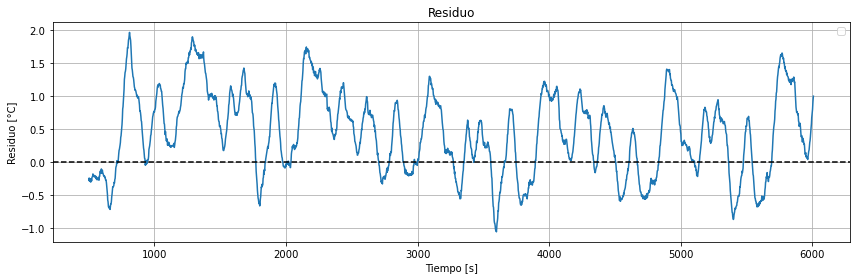
\includegraphics[width=\linewidth]{residuosNARXconnuevaTbase.png}
    \caption{Residuos del modelo NARX.}
    \label{fig:ResiduosNARX}
    \end{subfigure}
    \hfill
    \begin{subfigure}[b]{0.48\textwidth}
        \centering
        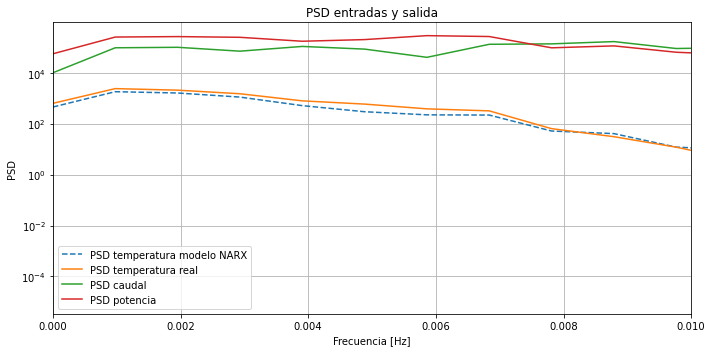
\includegraphics[width=\linewidth]{Figure 2026-07-07 230243 (8).png}
        \caption{Densidad espectral en el modelo NARX.}
        \label{fig:PSDNARXMISO}
    \end{subfigure}

    \vspace{0.4cm} % Espacio vertical entre filas

    % --- FILA 2: Correlaciones y Coherencia ---
    \begin{subfigure}[b]{0.31\textwidth}
        \centering
        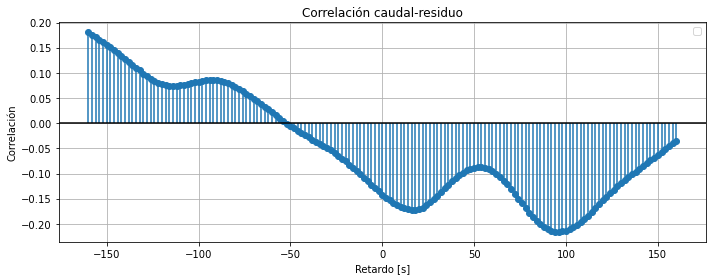
\includegraphics[width=\linewidth]{Figure 2026-07-07 230243 (14).png}
        \caption{Correlación caudal-residuos.}
        \label{fig:CorrelacionNARXCaudal}
    \end{subfigure}
    \hfill
    \begin{subfigure}[b]{0.31\textwidth}
        \centering
        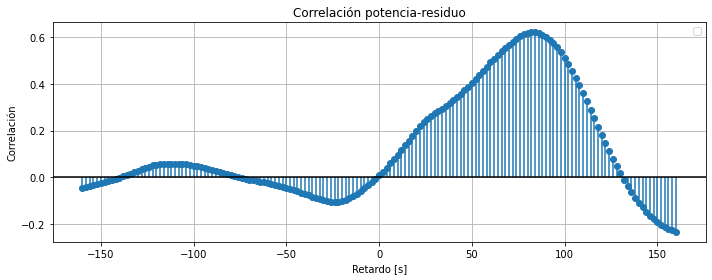
\includegraphics[width=\linewidth]{Figure 2026-07-07 230243 (15).png}
        \caption{Correlación potencia-residuos.}
        \label{fig:CorrelacionNARXpotencia}
    \end{subfigure}
    \hfill
    \begin{subfigure}[b]{0.31\textwidth}
        \centering
        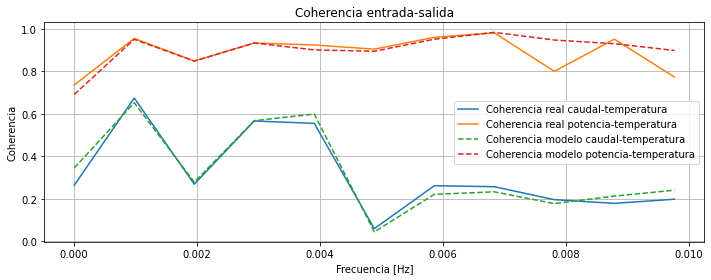
\includegraphics[width=\linewidth]{Figure 2026-07-07 230243 (12).png}
        \caption{Coherencia.}
        \label{fig:coherenciaNARX}
    \end{subfigure}

    \vspace{0.4cm}

    % --- FILA 3: Respuesta en Frecuencia (FRF) ---
    \begin{subfigure}[b]{0.48\textwidth}
        \centering
        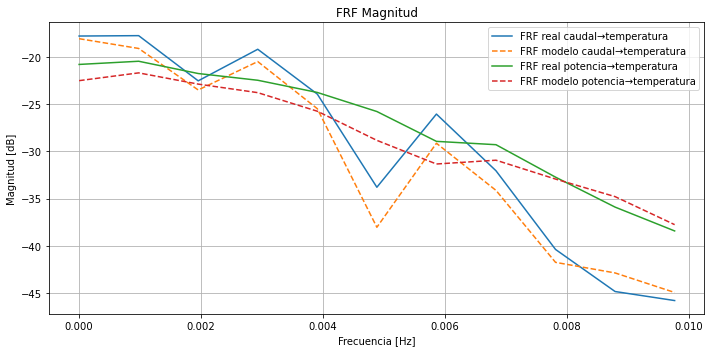
\includegraphics[width=\linewidth]{Figure 2026-07-07 230243 (11).png}
        \caption{FRF: Magnitud.}
        \label{fig:frfMAGNITUDNARXMISO}
    \end{subfigure}
    \hfill
    \begin{subfigure}[b]{0.48\textwidth}
        \centering
        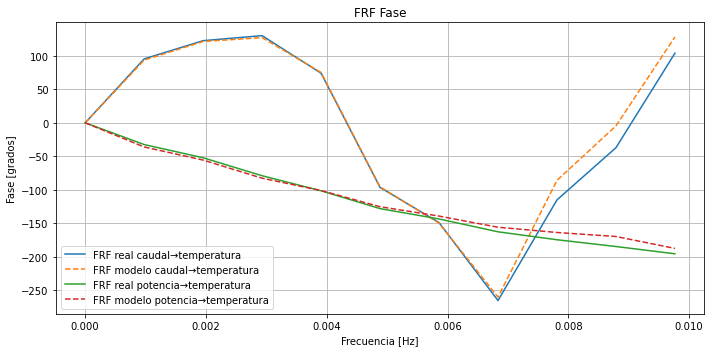
\includegraphics[width=\linewidth]{Figure 2026-07-07 230243 (10).png}
        \caption{FRF: Fase.}
        \label{fig:FRFFASENARXMISO}
    \end{subfigure}

    % Caption global de todo el bloque
    \caption{Validación y análisis espectral del modelo no lineal NARX MISO.}
    \label{fig:analisis_completo_NARX_MISO}
\end{figure}

En conjunto, los resultados muestran que el modelo NARX MISO polinomial logra capturar satisfactoriamente la forma oscilatoria y el contenido frecuencial de la respuesta térmica. Sin embargo, la subestimación de la temperatura recurrente en los máximos, los residuos no centrados en cero y la alta correlación entre potencia y residuo evidencian que aún permanecen dinámicas no explicadas por el modelo.

Por lo tanto, si bien el modelo NARX MISO constituye un avance respecto de las estructuras lineales, al incorporar relaciones no lineales e interacciones entre el caudal, la potencia y las salidas pasadas, su desempeño en simulación libre aún presenta limitaciones. En consecuencia, se evalúa una estructura no lineal alternativa basada en redes neuronales, con el propósito de mejorar la capacidad del modelo.


\subsection{Modelo de red neuronal con EDO}

Con el propósito de evaluar una estructura no lineal con mayor capacidad para representar la dinámica del sistema térmico, se implementó un modelo basado en ecuaciones diferenciales ordinarias neuronales, denominado Neural ODE. A diferencia de las estructuras discretas previamente analizadas, este enfoque no estima directamente la salida futura mediante una relación algebraica entre muestras, sino que aprende la evolución temporal del sistema a partir de una ecuación diferencial parametrizada mediante una red neuronal.

La estructura utilizada corresponde a una Neural ODE latente con configuración MISO, debido a que considera como entradas el caudal y la potencia eléctrica e incorpora, además de la salida normalizada, un conjunto de estados internos no medidos directamente. De forma general, la dinámica se representa mediante:


$$\frac{dx}{dt}=f_{\theta}(x,q_n(t-\tau_q),p_n(t-\tau_p))$$
Donde $x$ representa la vector de estados, $f_{\theta}$ corresponde a función no lineal aproximada por la red neuronal, $q_n$ es el caudal normalizado, $p_n$ es la potencia normalizada y $\tau_q$ y $\tau_p$ son los retardos asociados a cada entrada. A partir de esta formulación, la identificación del modelo se desarrolló mediante los siguientes pasos:

\begin{enumerate}
    \item \textbf{Construcción y selección de los datos utilizados}

    En primer lugar, se definió la variable de salida como la variación de temperatura respecto de la condición térmica registrada a los 500 segundos, al igual que en los anteriores modelos. A partir de este instante se seleccionaron los datos empleados en la identificación, excluyendo el transitorio térmico inicial del banco de ensayos. Posteriormente, los datos fueron divididos cronológicamente, destinando el 80 \% inicial al entrenamiento y el 20 \% restante a la validación. 

    \item \textbf{Normalización de las señales}

    Las señales de entrada se normalizaron utilizando la media y desviación estándar obtenidas a partir del conjunto de entrenamiento. La normalización permite reducir las diferencias de escala entre las variables y favorecer un mejor condicionamiento numérico durante el proceso de optimización. Si las variables fueran utilizadas directamente en sus unidades físicas, aquellas con mayores magnitudes numéricas podrían influir de manera desproporcionada sobre la actualización de los parámetros de la red

\item \textbf{Incorporación de los retardos de las entradas}


Una vez normalizadas las señales, se incorporaron retardos independientes para el caudal y la potencia. En el código se utilizaron  $\tau_q=54$ segundos para el caudal y $\tau_p=70$ segundos para la potencia eléctrica. Considerando un período de muestreo cercano a 2 segundos, estos valores corresponden aproximadamente a 27 y 35 muestras, respectivamente. Los retardos fueron definidos previamente a partir del análisis de correlación cruzada entre cada entrada y la salida.

La incorporación de estos retardos permite entregar a la red las entradas desplazadas temporalmente de acuerdo con la respuesta observada del sistema. Un retardo menor al adecuado presentaría a la red el efecto de una entrada de manera anticipada, mientras que un valor excesivamente grande retrasaría la información relevante. En ambos casos, el modelo debería compensar este desfase mediante su dinámica interna, dificultando el proceso de identificación.

\item \textbf{Definición del vector de estados latentes}

Posteriormente, se definió el vector de estados de la Neural ODE. Un estado latente corresponde a una variable interna del modelo que no se mide directamente en el sistema físico, sino que es aprendida durante el entrenamiento con el propósito de representar información dinámica que no puede describirse únicamente a partir de las variables observadas. En este caso, estos estados permiten aportar memoria interna al modelo y representar comportamientos asociados a la evolución térmica del sistema sin asignarles necesariamente una interpretación física específica.
En la implementación utilizada se definieron cuatro estados latentes adicionales a la variación de temperatura normalizada, por lo que el vector de estados quedó expresado como:

%$$x=[\Delta T_n,z_1,z_2,z_3,z_4,z_5,z_6]$$
$$x=[\Delta T_n,z_1,z_2,z_3,z_4]$$
De esta forma, el modelo posee cinco estados en total, donde $T_n$ corresponde a la variable de salida normalizada y $z_1,...,z_4$ representan los estados latentes. Estos últimos evolucionan conjuntamente con $T_n$  y permiten que la red neuronal almacene y utilice información sobre la dinámica pasada del sistema durante la integración temporal.

El número de estados latentes constituye un parámetro definido antes del entrenamiento. Una cantidad reducida disminuye la complejidad del modelo, pero puede limitar su capacidad para representar dinámicas internas, mientras que un número mayor incrementa su flexibilidad, aunque también aumenta el número de parámetros, el costo computacional y el riesgo de sobreajuste. En este trabajo se utilizaron cuatro estados latentes buscando un equilibrio entre capacidad de representación y complejidad computacional y del modelo.


\item \textbf{Definición de la función que representa la EDO}

La red neuronal recibe en cada instante los cinco estados del sistema junto con las dos entradas retardadas, por lo que su dimensión de entrada es igual a siete. La estructura seleccionada posee tres capas ocultas de 64 neuronas cada una. La capa de salida contiene cinco neuronas, correspondientes a las derivadas temporales de los cinco estados. Por lo tanto, la arquitectura utilizada puede representarse como:

$$7\rightarrow64\rightarrow64\rightarrow64\rightarrow5$$


El número de capas y neuronas corresponde a parámetros definidos previamente al entrenamiento. Una red de menor tamaño posee menor costo computacional, aunque puede disponer de una capacidad insuficiente para representar relaciones no lineales complejas. Por el contrario, una arquitectura excesivamente grande aumenta el número de parámetros y puede favorecer el sobreajuste. La configuración utilizada busca mantener una capacidad no lineal suficiente sin incrementar excesivamente la complejidad del modelo ni los costos computacionales.

Las cinco salidas de esta red no corresponden directamente a los estados siguientes, sino a sus derivadas temporales:
$$f_\theta(\cdot) = \begin{bmatrix}
\frac{d\Delta T_n}{dt} \\[6pt]
\frac{dz_1}{dt} \\[2pt]
\vdots \\[2pt]
\frac{dz_4}{dt}
\end{bmatrix}.$$

Es en este punto donde el código construye propiamente la EDO neuronal: la red aprende la función que relaciona el estado actual y las entradas con la velocidad de cambio de cada uno de los estados. Durante el entrenamiento, los pesos y sesgos de la red son modificados para que estas derivadas generen posteriormente una trayectoria de temperatura próxima a la experimental.
En la formulación también se incorpora un término de amortiguamiento sobre los estados para favorecer la estabilidad numérica durante integraciones prolongadas.

\item \textbf{Cálculo de la evolución temporal mediante integración de la EDO}

Después de que la red calcula las derivadas, estas deben integrarse para obtener el estado en el instante siguiente. El código utiliza el método de Runge-Kutta de cuarto orden, RK4, para resolver numéricamente la EDO durante cada intervalo de muestreo. Por lo tanto, en cada paso temporal ocurre la siguiente secuencia:

$$(x_k,q_k,p_k)\rightarrow f_\theta\rightarrow\frac{dx}{dt}\rightarrow RK4\rightarrow x_{k+1}$$

Este procedimiento se repite de manera recursiva a lo largo de toda la trayectoria. 

\item \textbf{Primera etapa de entrenamiento mediante ventanas crecientes}

Una vez definida la ecuación diferencial neuronal y el procedimiento de integración, se inició el entrenamiento de los parámetros $\theta$ de la red, el cual representa el conjunto de parámetros ajustables del modelo, principalmente los pesos y sesgos de las capas neuronales, además de los parámetros internos asociados al término de amortiguamiento. Estos valores determinan la forma de la función $f_\theta$ y, por tanto, la manera en que la red calcula las derivadas temporales de los estados. Durante el entrenamiento, $\theta$ se modifica iterativamente con el objetivo de que las trayectorias generadas por la Neural ODE reproduzcan adecuadamente la evolución experimental de $\Delta T$.

Para realizar este ajuste, el conjunto de entrenamiento se divide temporalmente en ventanas, entendidas como segmentos continuos de datos que contienen una secuencia de valores de caudal, potencia y temperatura durante un determinado intervalo. En cada ventana se selecciona un instante inicial y, a partir de este, se toman consecutivamente las muestras correspondientes a la longitud establecida. Por ejemplo, una ventana de 200 muestras representa aproximadamente 400 segundos para un período de muestreo de 2 segundos.

En cada entrenamiento, el código selecciona aleatoriamente ventanas dentro del conjunto de datos. Para cada una de ellas, se utiliza el valor inicial de $\Delta T_n$ como condición inicial, mientras que los estados latentes comienzan desde cero. A continuación, la Neural ODE calcula las derivadas de los estados y estas se integran sucesivamente mediante RK4 durante toda la ventana. De este modo, se obtiene una trayectoria simulada de $\Delta T_n$, que se compara con la trayectoria experimental correspondiente al mismo intervalo. El error obtenido se utiliza posteriormente para actualizar los parámetros $\theta$ de la red.

La utilización de ventanas permite entrenar el modelo sobre diferentes sectores de la trayectoria experimental sin tener que integrar la totalidad del registro en cada actualización de los parámetros. Además, al seleccionar diferentes posiciones iniciales, la red aprende la dinámica bajo distintas condiciones presentes en el conjunto de entrenamiento y no solamente a partir de una única trayectoria iniciada siempre en el mismo punto.

En esta primera etapa, la longitud de las ventanas aumenta progresivamente desde 200 hasta 900 muestras. Esto permite que el modelo comience aprendiendo la dinámica sobre horizontes relativamente cortos y, a medida que avanza el entrenamiento, deba reproducir trayectorias cada vez más prolongadas. Si las ventanas fueran demasiado cortas durante todo el proceso, el modelo podría reproducir adecuadamente cambios locales pero acumular errores en simulaciones extensas. Por el contrario, utilizar ventanas muy largas desde el comienzo aumentaría la dificultad de la optimización, ya que los errores y gradientes deben propagarse a través de una cantidad mayor de pasos de integración.

\item \textbf{Definición de la función de pérdida}

En cada ventana de entrenamiento se calcula una función de pérdida cuyo término principal corresponde al error cuadrático medio entre la variación de temperatura simulada y la experimental. A este término se agregan penalizaciones de baja intensidad asociadas a la magnitud de las derivadas y de los estados latentes. Estas penalizaciones actúan como mecanismos de regularización.

\item \textbf{Actualización de los parámetros de la EDO neuronal}

Una vez obtenida la trayectoria simulada para cada ventana, se calcula la diferencia entre la respuesta del modelo y la variación de temperatura experimental mediante la función de pérdida definida previamente. A partir de este error se determinan los gradientes, que indican en qué dirección y magnitud deben modificarse los parámetros $\theta$ de la red para disminuir la pérdida. La actualización de los parámetros de la red se realizó ajustándolos progresivamente para reducir la diferencia entre la respuesta simulada y la experimental. En una primera etapa se permitió un ajuste más amplio del modelo y, posteriormente, se realizó un afinamiento con modificaciones de menor magnitud. Además, se incorporó una limitación en las actualizaciones para favorecer la estabilidad durante el entrenamiento. De esta manera, la actualización de los parámetros se realiza progresivamente hasta obtener una función $f_\theta$ capaz de generar, mediante su integración, una evolución de $\Delta T $representativa de los datos experimentales.


\item \textbf{Segunda etapa de entrenamiento}

Se realizó un segundo entrenamiento destinado específicamente a mejorar el comportamiento del modelo durante simulaciones de mayor duración. Para ello se utilizaron segmentos temporales de 1200 muestras, equivalentes aproximadamente a 2400 segundos para un período de muestreo cercano a 2 segundos. 

El propósito de utilizar trayectorias más largas es obligar al modelo a mantener una respuesta adecuada durante períodos prolongados. En una simulación libre, los errores generados en los primeros instantes pueden propagarse a los estados posteriores, produciendo una separación progresiva entre la respuesta simulada y la experimental. Por esta razón, esta segunda etapa busca reducir especialmente este tipo de deriva acumulada.

Además, el error no se pondera de manera uniforme a lo largo de la trayectoria. El código asigna pesos que aumentan progresivamente al final de cada segmento. Esto significa que los errores producidos hacia el final de una simulación prolongada tienen mayor influencia en el ajuste de los parámetros. Así, el entrenamiento favorece modelos capaces de conservar una respuesta adecuada no solo en los primeros instantes, sino también después de períodos extensos de integración.

\item \textbf{Selección de los parámetros finales y obtención de la salida del modelo}

Durante ambas etapas de entrenamiento, el código registra continuamente el valor de la función de pérdida. Cada vez que se obtiene un valor menor al alcanzado anteriormente, se conserva una copia de los parámetros $\theta$ correspondientes a ese resultado. Al finalizar cada etapa se recupera el conjunto de parámetros asociado al menor error observado, evitando utilizar necesariamente los valores obtenidos en la última iteración del entrenamiento.

Una vez finalizado el entrenamiento, estos parámetros determinan la función $f_\theta$ que describe las derivadas temporales de los estados. Para generar una respuesta, la red calcula dichas derivadas a partir del estado actual, el caudal retardado y la potencia retardada; posteriormente, el método RK4 las integra para obtener el nuevo estado. Este proceso se repite sucesivamente a lo largo del tiempo.

La Neural ODE no entrega directamente la temperatura como salida de la red neuronal. La red calcula primero las derivadas de los estados, estas se integran para obtener su evolución temporal y, finalmente, el primer estado integrado proporciona la estimación de $\Delta T$.

\item \textbf{Evaluación del modelo}

Una vez finalizado el entrenamiento, el modelo fue evaluado mediante simulación libre tanto sobre el conjunto de entrenamiento como sobre el de validación. %La respuesta obtenida se evaluó mediante RMSE, MAE, $R^2$ y FIT, complementándose el análisis mediante la comparación temporal, densidad espectral de potencia y correlación entre los residuos y las entradas.


\end{enumerate}

En síntesis, la identificación de la Neural ODE consiste en aprender una función $f_\theta$ que determina las derivadas temporales de la temperatura normalizada y de los estados latentes. Estas derivadas son integradas mediante RK4 para generar la trayectoria del sistema, la cual se compara con los datos experimentales para actualizar iterativamente los parámetros de la red. De esta manera, el proceso de entrenamiento no busca directamente una relación algebraica entre entradas y salida, sino una representación continua de la dinámica que, al ser integrada en el tiempo, permita reproducir la evolución térmica observada y posteriormente operar en simulación libre.






\subsubsection{Simulación libre}


El desempeño del modelo ODE neuronal se evaluó mediante simulación libre, utilizando únicamente las señales de entrada de caudal y potencia para propagar la respuesta del modelo, sin realimentar la temperatura experimental. Los resultados obtenidos fueron un RMSE de 0.818 °C, un MAE de 0.677 °C, un coeficiente de determinación $R^2$=0.914 y un índice FIT de 70.64\%. Estos valores indican que el modelo reproduce adecuadamente la tendencia general y una proporción importante de la variabilidad de la temperatura experimental, aunque todavía presenta diferencias sistemáticas en determinados intervalos de operación.

\begin{figure}[H]
    \centering
    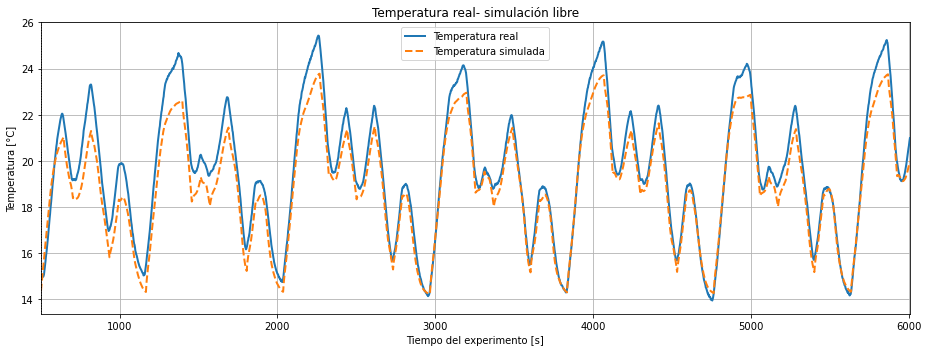
\includegraphics[width=0.65\linewidth]{Figure 2026-07-09 235930 (23).png}
    \caption{Gráfico de comparación de temperatura real y temperatura simulada.}
    \label{fig:SIMLIBREODEneuronal}
\end{figure}




El análisis temporal de los residuos (Figura \ref{fig:residuosODE}) muestra que estos permanecen mayoritariamente por encima de cero y alcanzan valores cercanos a 2 °C en algunos sectores. Considerando que el residuo se define como la diferencia entre la temperatura real y la simulada, este comportamiento indica que el modelo tiende, en general, a subestimar la temperatura del sistema. Además, los residuos presentan oscilaciones estructuradas y de baja frecuencia, en lugar de distribuirse aleatoriamente alrededor de cero. Por tanto, aunque el modelo logra representar la dinámica principal, todavía existen componentes determinísticas que no han sido completamente capturadas.
La comparación de las densidades espectrales de potencia (Figura \ref{fig:PSDODEneuronal}) muestra una elevada similitud entre la temperatura real y la temperatura simulada dentro de la banda de interés. Ambas curvas presentan prácticamente la misma tendencia decreciente y niveles de energía comparables. Este resultado indica que el modelo reproduce adecuadamente la distribución frecuencial de la salida y, en particular, la dinámica lenta predominante del sistema térmico.
Los resultados de coherencia (Figura \ref{fig:coherenciaODE}) también muestran una correspondencia entre el sistema real y el modelo. En la relación potencia–temperatura, la coherencia es elevada en prácticamente toda la banda analizada. Las curvas obtenidas con la temperatura real y simulada son muy similares, lo que confirma que el modelo representa adecuadamente el efecto de la potencia eléctrica sobre la respuesta térmica. Para la relación caudal–temperatura, en cambio, la coherencia presenta valores menores y una variación más pronunciada con la frecuencia. No obstante, las curvas real y simulada conservan una forma semejante, por lo que el modelo reproduce razonablemente la contribución del caudal, aunque esta relación es menos dominante y más difícil de identificar que la asociada a la potencia.
En magnitud, las FRF obtenidas (Figura \ref{fig:FRFmagnitudODE}) para la temperatura real y simulada presentan una concordancia satisfactoria para ambas entradas. La ganancia disminuye al aumentar la frecuencia, comportamiento consistente con la naturaleza de baja frecuencia del sistema térmico. La correspondencia es especialmente clara en la relación potencia–temperatura. En el caso del caudal, las diferencias son reducidas en gran parte de la banda, aunque aumentan ligeramente en las frecuencias más altas. En la fase (Figura \ref{fig:FRFfaseODE}) también se observa una buena coincidencia entre la respuesta real y simulada, particularmente para la entrada de caudal. Para la potencia, ambas respuestas presentan una tendencia similar, aunque aparecen diferencias en la zona de frecuencias superiores, lo cual sugiere que el modelo podría no reproducir completamente algunos retardos o transiciones dinámicas de la respuesta térmica en esa región frecuencial.

El análisis de correlación cruzada entre los residuos y las entradas (Figuras \ref{fig:correlacionRESIDUOSCAUDALode} y \ref{fig:correlacionRESIDUOSPOTENCIAODE}) permite evaluar si todavía existe información de las señales de excitación contenida en el error. Para el caudal, las correlaciones son generalmente moderadas, aunque se observan algunos máximos cercanos a 0.15. Esto indica que parte del efecto dinámico del caudal no ha sido totalmente incorporado por el modelo. En el caso de la potencia, las correlaciones son más elevadas y alcanzan valores superiores a 0.4 para ciertos retardos. En consecuencia, los residuos no pueden considerarse completamente independientes de las entradas, especialmente de la potencia. Este resultado revela que, a pesar de la elevada coherencia y la adecuada reproducción espectral, todavía permanece una componente predecible en el error que podría reducirse mediante un ajuste adicional de la estructura o del procedimiento de entrenamiento.


\begin{figure}[H]
    \centering
    % ---- Fila 1 ----
    \begin{subfigure}[b]{0.48\linewidth}
        \centering
        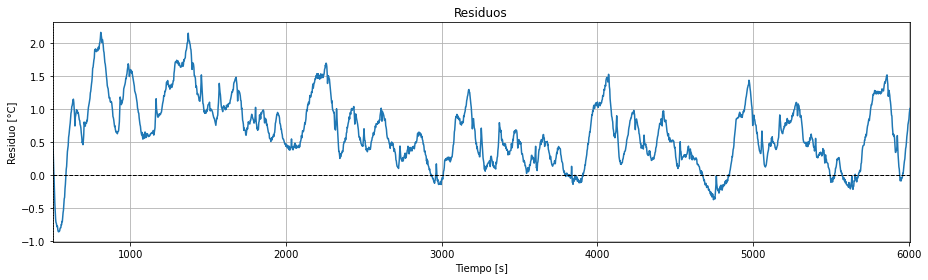
\includegraphics[width=\linewidth]{Figure 2026-07-09 235930 (1).png}
        \caption{Residuos del modelo EDO neuronal.}
        \label{fig:residuosODE}
    \end{subfigure}
    \hfill
    \begin{subfigure}[b]{0.48\linewidth}
        \centering
        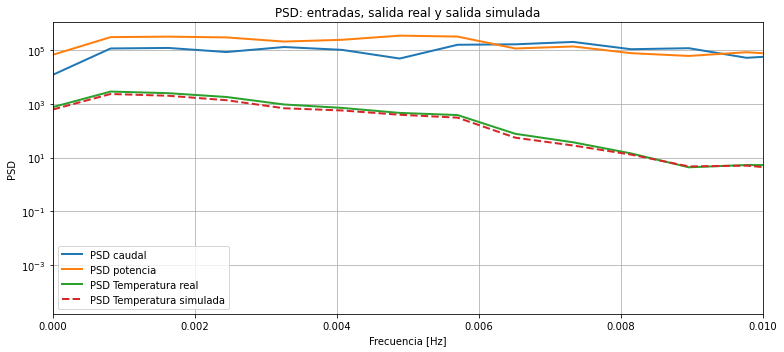
\includegraphics[width=\linewidth]{Figure 2026-07-09 235930 (2).png}
        \caption{Densidad espectral.}
        \label{fig:PSDODEneuronal}
    \end{subfigure}
    
    \vspace{0.5cm} % Espacio vertical entre filas

    % ---- Fila 2 ----
    \begin{subfigure}[b]{0.48\linewidth}
        \centering
        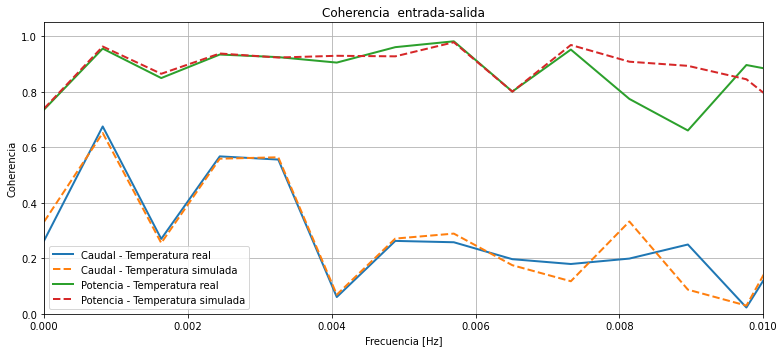
\includegraphics[width=\linewidth]{Figure 2026-07-09 235930 (3).png}
        \caption{Coherencia espectral.}
        \label{fig:coherenciaODE}
    \end{subfigure}
    \hfill
    \begin{subfigure}[b]{0.48\linewidth}
        \centering
        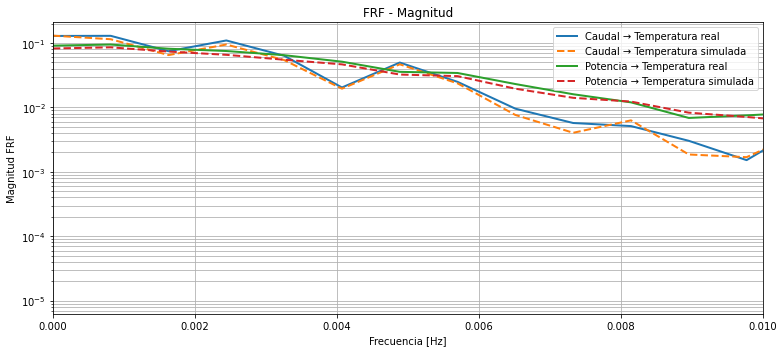
\includegraphics[width=\linewidth]{Figure 2026-07-09 235930 (4).png}
        \caption{FRF: Magnitud.}
        \label{fig:FRFmagnitudODE}
    \end{subfigure}

    \vspace{0.5cm}

    % ---- Fila 3 ----
    \begin{subfigure}[b]{0.48\linewidth}
        \centering
        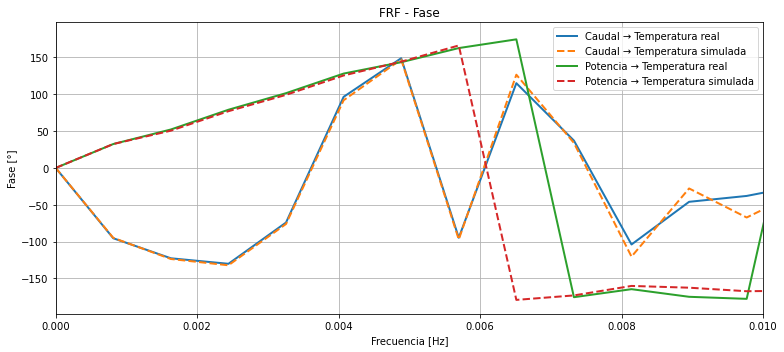
\includegraphics[width=\linewidth]{Figure 2026-07-09 235930 (5).png}
        \caption{FRF: Fase.}
        \label{fig:FRFfaseODE}
    \end{subfigure}
    \hfill
    \begin{subfigure}[b]{0.48\linewidth}
         \centering
    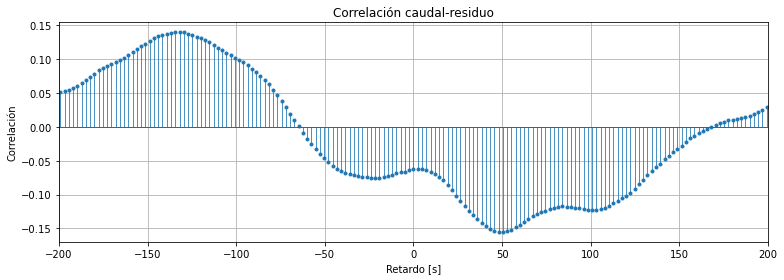
\includegraphics[width=\linewidth]{caudalresiduoEDONEURONAL.png}
    \caption{Correlación entre el caudal y los residuos.}
    \label{fig:correlacionRESIDUOSCAUDALode}
    \end{subfigure}

    \vspace{0.5cm}

    % ---- Fila 4 (Última imagen centrada) ----
    \begin{subfigure}[b]{0.48\linewidth}
       \centering
    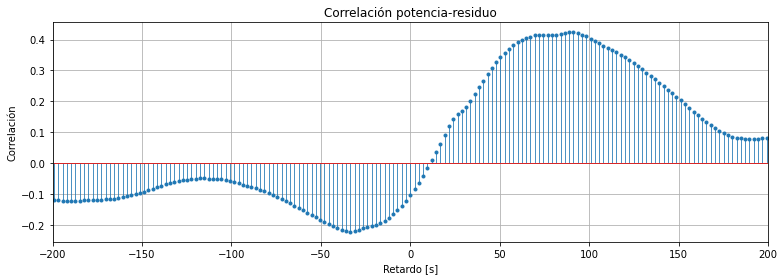
\includegraphics[width=\linewidth]{potenciaresiduoEDONEURONAL.png}
    \caption{Correlación entre la potencia y los residuos.}
    \label{fig:correlacionRESIDUOSPOTENCIAODE}
    \end{subfigure}

    % Título y etiqueta global para todo el grupo de imágenes
    \caption{Análisis y diagnóstico del modelo EDO neuronal.}
    \label{fig:analisisCompletoODE}
\end{figure}

\subsection{Conclusión de modelos MISO}


La evaluación de los modelos MISO permitió analizar la capacidad de distintas estructuras para representar la dinámica térmica del banco de ensayos considerando simultáneamente el caudal y la potencia eléctrica como entradas, y la variación de temperatura como salida. Esta formulación permitió incorporar de manera conjunta los efectos hidráulicos y térmicos que influyen sobre la respuesta del sistema, mostrando que la potencia eléctrica constituye la entrada con mayor influencia directa, mientras que el efecto del caudal es más débil, retardado y dependiente de la frecuencia.

El modelo Box-Jenkins MISO presentó el desempeño más deficiente en simulación libre. Aunque su estructura lineal permitió representar parcialmente algunas oscilaciones de baja frecuencia, no logró reproducir adecuadamente el nivel medio, la amplitud ni el desfase de la temperatura experimental. Los indicadores obtenidos (Tabla \ref{tab:metricas_modelosMISO}) evidenciaron que el modelo no fue capaz de generalizar satisfactoriamente en simulación libre. Asimismo, los residuos presentaron un sesgo importante y una estructura persistente, mientras que las correlaciones entre las entradas y el error mostraron la presencia de dinámica no explicada, especialmente asociada a la potencia. En consecuencia, la estructura lineal Box-Jenkins resultó insuficiente para representar la complejidad del sistema MISO.


Frente a estas limitaciones, el modelo NARX MISO permitió mejorar significativamente el desempeño al incorporar términos no lineales, interacciones entre variables y dependencias autorregresivas. El modelo identificado alcanzó las métricas observadas en la Tabla \ref{tab:metricas_modelosMISO}, las cuales muestran que el NARX logró reproducir adecuadamente la forma oscilatoria, la periodicidad y gran parte de la variabilidad de la temperatura experimental. No obstante, se observó una subestimación recurrente en algunos máximos de temperatura, junto con residuos estructurados y una correlación elevada entre la potencia y el error. Esto indica que, si bien el modelo representa satisfactoriamente la dinámica dominante, todavía existen componentes térmicas y retardos efectivos que no fueron completamente capturados

El modelo basado en una EDO neuronal latente también presentó un desempeño satisfactorio en simulación libre. Los indicadores obtenidos (Tabla \ref{tab:metricas_modelosMISO}), si bien fueron inferiores a los alcanzados por el modelo NARX, mostraron una adecuada capacidad de reproducir el contenido temporal y frecuencial de la salida.  La similitud observada entre las PSD, las coherencias y las FRF reales y simuladas indica que esta estructura logró representar correctamente la dinámica lenta predominante del sistema y la relación frecuencial entre las entradas y la temperatura. Sin embargo, la presencia de residuos mayoritariamente positivos y correlacionados con las entradas, especialmente con la potencia, evidencia que aún permanecen componentes predecibles no explicados por el modelo.

\begin{table}[H]
\centering
\caption{Métricas de rendimiento y ajuste de los modelos MISO.}
\label{tab:metricas_modelosMISO}
\begin{tabular}{|l|l|l|l|l|}
\hline
Modelo           & RMSE(°C) & MAE   & $R^2$ & FIT \%       \\ \hline
Box-Jenkins MISO & 4.109    & 3.261 & -1.173             & -47.410 \\ \hline
NARX             & 0.756    & 0.614 & 0.927                & 72.92   \\ \hline
Red Neuronal EDO & 0.818    & 0.677 & 0.914                & 70.64   \\ \hline
\end{tabular}
\end{table}

En términos comparativos, el modelo NARX MISO presentó el mejor desempeño temporal entre las estructuras evaluadas, al obtener los menores errores y los mayores valores de $R^2$ y FIT. La EDO neuronal mostró resultados cercanos y una representación frecuencial consistente, además de ofrecer una formulación más flexible para describir dinámicas internas mediante estados latentes. Por su parte, el modelo Box-Jenkins MISO no logró representar apropiadamente el comportamiento del sistema en simulación libre, confirmando que las estructuras lineales evaluadas en este trabajo no fueron suficientes para describir adecuadamente las interacciones entre caudal, potencia y temperatura.

Los resultados obtenidos sugieren la presencia de un comportamiento predominantemente no lineal y multivariable dentro del rango de operación estudiado, cuya representación requiere modelos capaces de incorporar interacciones entre entradas, retardos y dependencias dinámicas complejas. Entre las estructuras analizadas, el modelo NARX MISO constituye la alternativa más adecuada para la simulación libre del sistema, debido a su mayor precisión temporal y menor error de estimación. No obstante, la EDO neuronal representa una alternativa prometedora, especialmente por su capacidad para modelar estados internos no medidos y reproducir la dinámica frecuencial del proceso. En ambos casos, la correlación residual con la potencia indica que aún existe margen de mejora en la representación del aporte térmico, los retardos distribuidos y la acumulación de energía en el banco de ensayos.




\chapter{Conclusión e investigación futura} 

\section{Conclusiones}

%En este trabajo se analizó un sistema térmico de emulación termosolar a escala reducida, con el propósito de desarrollar un modelo computacional capaz de representar su comportamiento dinámico no estacionario a partir de datos experimentales obtenidos directamente del banco de ensayos. Para ello, se realizó una revisión de distintas estructuras de identificación basadas en datos, incluyendo modelos lineales y no lineales, junto con el estudio de las condiciones necesarias para obtener conjuntos de datos suficientemente informativos. A partir de este análisis, se seleccionaron señales PRBS y multisinusoidales para excitar de manera controlada las entradas del sistema. En una primera etapa se consideró únicamente el caudal como variable manipulada, obteniéndose modelos SISO cuya salida correspondió a la temperatura del fluido. Posteriormente, se incorporó la potencia eléctrica suministrada por las resistencias como una segunda entrada, lo que permitió obtener conjuntos de datos MISO más representativos y llevar al sistema a condiciones de operación más cercanas a su comportamiento real.

La revisión del estado del arte permitió establecer los principales lineamientos metodológicos para la identificación del sistema térmico de emulación termosolar. A partir de este análisis, se determinó la conveniencia de evaluar modelos basados en datos, tanto lineales como no lineales, capaces de representar la dinámica del sistema sin formular ecuaciones termodinámicas y de transferencia de calor. Para la modelación lineal se seleccionaron las estructuras autorregresiva con entradas exógenas (ARX), Output Error (OE) y Box-Jenkins (BJ), mientras que para la representación no lineal se consideraron el modelo NARX y un modelo basado en ecuaciones diferenciales ordinarias y redes neuronales. Asimismo, la revisión permitió identificar las señales binarias pseudoaleatorias (PRBS) y multisinusoidales como alternativas apropiadas para excitar la dinámica del sistema y obtener conjuntos de datos suficientemente informativos para su identificación.


El análisis temporal y frecuencial de las señales permitió caracterizar el comportamiento dinámico del banco de ensayos. Los resultados mostraron que el sistema presenta una dinámica predominantemente lenta, concentrada principalmente en el intervalo comprendido entre 0 y 0.01 Hz. Además, se estableció que la potencia eléctrica es la entrada con mayor influencia sobre la temperatura de salida, debido a que su efecto térmico se manifiesta de manera directa. El caudal también influye sobre la respuesta del sistema, aunque su efecto es de menor magnitud, más indirecto y dependiente de la frecuencia.

El desarrollo de los modelos se efectuó progresivamente, comenzando con estructuras lineales SISO, en las que se consideró el caudal como entrada y la temperatura como salida. Los modelos ARX, OE y BJ presentaron limitaciones en simulación libre, evidenciadas en diferencias de amplitud y evolución temporal respecto de la respuesta experimental. Posteriormente, se desarrolló una estructura lineal MISO mediante la incorporación de la potencia eléctrica como segunda entrada al modelo Box-Jenkins. Sin embargo, esta ampliación no produjo una mejora significativa, lo que indicó que las interacciones entre las variables no podían ser representadas adecuadamente mediante una relación exclusivamente lineal. Finalmente, se evaluaron estructuras MISO no lineales, específicamente un modelo NARX y un modelo neuronal basado en ecuaciones diferenciales ordinarias. Entre ellas, el NARX presentó el mejor desempeño global. Conceptualmente, este resultado se atribuye a su capacidad para representar relaciones no lineales y dependencias temporales mediante valores pasados de las entradas y de la propia salida, lo que le permitió capturar de mejor manera los retardos, la acumulación térmica y las interacciones entre el caudal, la potencia eléctrica y la temperatura.

En simulación libre, el modelo NARX reprodujo satisfactoriamente la tendencia oscilatoria, la variabilidad y una parte importante del contenido frecuencial de la temperatura, alcanzando un RMSE de 0.76 °C, un MAE de 0.61 °C, un coeficiente de determinación de 0.93 y un FIT de 72.9 \%. El modelo neuronal basado en ecuaciones diferenciales ordinarias también presentó resultados satisfactorios, con un RMSE de 0.82 °C y un FIT de 70.6 \%, aunque su desempeño temporal fue ligeramente inferior. No obstante, el análisis de los residuos mostró la presencia de correlaciones con las señales de entrada, especialmente con la potencia eléctrica. Esto indica que aún existen componentes de la dinámica que no fueron capturadas completamente, posiblemente asociadas con retardos distribuidos, acumulación térmica, pérdidas de calor o interacciones no lineales de mayor complejidad. Por tanto, aunque el NARX proporcionó la mejor representación entre las estructuras estudiadas, todavía existe margen para perfeccionar su configuración y el diseño de las señales de excitación.

En consecuencia, se considera que el objetivo general de desarrollar un modelo computacional basado en datos experimentales que represente el comportamiento dinámico no estacionario del sistema térmico de emulación termosolar fue alcanzado. En primer lugar, se obtuvo una caracterización temporal y frecuencial del sistema mediante señales de excitación diseñadas específicamente para generar datos informativos. En segundo lugar, se desarrolló y validó en simulación libre un modelo capaz de reproducir la respuesta térmica frente a variaciones simultáneas del caudal y de la potencia eléctrica, sin utilizar de forma explícita ecuaciones termodinámicas ni de transferencia de calor. Además, la comparación sistemática de estructuras SISO y MISO, lineales y no lineales, permitió seleccionar al modelo NARX como la alternativa de mejor desempeño bajo las condiciones experimentales consideradas. Sin embargo, su capacidad predictiva debe limitarse al rango de operación utilizado durante la identificación y validación, debido a que la correlación remanente entre las entradas y los residuos evidencia la necesidad de ampliar los conjuntos de datos, perfeccionar el diseño experimental y continuar mejorando la estructura del modelo.


\section{Investigaciones futuras}


A partir de los resultados obtenidos y de las limitaciones identificadas durante el desarrollo de esta investigación, se proponen distintas líneas de trabajo futuro orientadas a mejorar la capacidad de representación y generalización de los modelos.

En primer lugar, se recomienda validar el modelo NARX utilizando conjuntos de datos obtenidos en diferentes épocas del año. Los experimentos utilizados para la identificación y validación de los modelos MISO fueron realizados durante el invierno, por lo que una validación con datos obtenidos en verano permitiría someter al modelo a condiciones térmicas y ambientales distintas. Esto contribuiría a evaluar con mayor rigurosidad su capacidad de generalización y su desempeño fuera de las condiciones utilizadas durante la identificación.

También resulta conveniente diseñar nuevas señales MISO que presenten una menor correlación y coherencia entre las entradas. Una mayor independencia entre el caudal y la potencia permitiría separar con mayor claridad el efecto individual de cada variable sobre la temperatura. Para ello, sería recomendable realizar un número mayor de experimentos, considerar diferentes puntos de operación y evaluar nuevas combinaciones de señales PRBS y multisinusoidales.

Otra línea de investigación consiste en controlar de manera independiente cada una de las resistencias eléctricas del banco de ensayos. En los experimentos realizados, todas las resistencias variaron simultáneamente, lo que limitó la posibilidad de analizar la distribución espacial del aporte térmico. La manipulación independiente de cada resistencia permitiría reproducir de forma más realista la distribución no uniforme de irradiancia que puede presentarse en una instalación termosolar y generaría información adicional sobre la propagación del calor a lo largo del sistema.

Dado el carácter exploratorio de este trabajo, orientado a comparar el desempeño relativo de distintas estructuras de modelado, se propone incorporar en futuras investigaciones un análisis de incertidumbre asociado a los instrumentos utilizados para la adquisición de datos. La cuantificación de los errores de medición permitiría evaluar en qué medida la precisión de sensores, caudalímetros y demás instrumentos afecta la calidad de los datos empleados en la identificación y, en consecuencia, el desempeño de los modelos obtenidos. Este análisis contribuiría a distinguir entre las limitaciones propias de la estructura del modelo y aquellas asociadas a la calidad de las mediciones experimentales. En la misma línea, dado el carácter exploratorio de este trabajo, se priorizó la amplitud de la comparación sobre un análisis estadístico profundo de cada estructura individual. Por esta razón, se recomienda, como línea de continuación, analizar la robustez estadística de los resultados obtenidos, evaluando entre las distintas estructuras las variaciones en los datos utilizados y su efecto en los modelos generados.

Asimismo, se podrían incorporar nuevas variables de entrada al modelo MISO, como la temperatura ambiente y la temperatura de entrada del fluido. La inclusión de estas variables permitiría representar de manera más completa las condiciones térmicas del sistema y reducir la influencia de perturbaciones no consideradas.

Se propone profundizar en la incidencia que tienen los órdenes y coeficientes sobre el desempeño de una misma estructura de modelos lineales. Para ello, se deberían comparar distintas configuraciones, ampliar las mallas de búsqueda utilizadas durante la identificación y analizar cómo las variaciones en los órdenes modifican los coeficientes estimados y las métricas de desempeño. Este estudio permitiría determinar si el aumento de complejidad dentro de una misma familia de modelos produce mejoras significativas o si, por el contrario, existen configuraciones más simples capaces de entregar un desempeño equivalente.

En relación con las estructuras de modelado, se recomienda explorar nuevas configuraciones NARX, incluyendo distintos órdenes, retardos, grados polinomiales y criterios de regularización. También podrían evaluarse modelos NARX basados en redes neuronales, capaces de representar relaciones no lineales más complejas sin depender exclusivamente de una expansión polinomial. Para el modelo ODE neuronal, sería conveniente estudiar diferentes números de estados latentes, arquitecturas de red, funciones de activación, estrategias de entrenamiento y términos de regularización. Estas modificaciones podrían mejorar la estabilidad de la simulación libre y reducir la correlación residual con las entradas.

Ligado con lo anterior, se recomienda complementar futuras investigaciones mediante la comparación del desempeño de los modelos obtenidos con resultados reportados en la literatura para sistemas térmicos de características similares. Esta comparación permitiría contextualizar las métricas alcanzadas, identificar posibles brechas de desempeño y evaluar si las estructuras desarrolladas presentan resultados consistentes con otros enfoques de identificación, considerando las diferencias en condiciones experimentales, variables empleadas y criterios de validación.

Otra alternativa consiste en incorporar conocimiento físico al proceso de identificación mediante modelos de caja gris. En este enfoque, las ecuaciones de balance de energía, las pérdidas térmicas, la capacidad térmica de los componentes y el transporte del fluido podrían combinarse con parámetros estimados a partir de datos. Esto permitiría mejorar la interpretabilidad física del modelo, aumentar su capacidad de extrapolación y reducir las dinámicas no explicadas observadas en los residuos.

Finalmente, se propone utilizar el modelo seleccionado como base para el diseño de estrategias de control. Entre las aplicaciones posibles se encuentran el control predictivo de la temperatura, la regulación del caudal, la gestión de la potencia eléctrica y la optimización energética del sistema. De esta manera, el modelo desarrollado no solo serviría para representar el comportamiento dinámico del banco de ensayos, sino también como herramienta para mejorar su operación y eficiencia.

















%El análisis del estado del arte permitió identificar una amplia variedad de enfoques de modelado dinámico aplicados a sistemas térmicos bajo condiciones operativas complejas y no lineales, donde existe alta variabilidad y restricciones operativas estrictas. A diferencia de los enfoques tradicionales, estas técnicas no requieren una estructura funcional predeterminada del proceso, permitiendo mayor flexibilidad y adaptabilidad frente a condiciones reales de operación.

%Dentro de las técnicas revisadas, se destacan los modelos estructurados como Hammerstein, Wiener y sus variantes combinadas, que ofrecen una representación modular de la dinámica y la no linealidad del sistema. De igual forma, se identificaron modelos avanzados basados en redes neuronales, como NARX, LSTM y ANN profundas, que han demostrado alta capacidad predictiva, aunque con una mayor exigencia en términos de calidad y volumen de datos. También se analizaron modelos de caja negra y caja gris, que permiten mejorar la precisión cuando existe ruido, incertidumbre o información física parcial del sistema.

%La modelación basada en datos requiere una adecuada identificación del sistema a modelar. Para ello,la señal de excitación utilizada debe ser capaz de relevar la dinámica relevante del sistema aportando información en la banda de frecuencias donde ocurren los fenómenos dominantes. Así, se diseñaron y ejecutaron excitaciones mediante dos tipos de señales de entrada: PRBS y multisinusoidal. Los primeros experimentos demostraron que la variación en la amplitud del caudal no modifica de manera apreciable la dinámica del sistema dentro de la banda de interés, lo que implica que experimentar variando únicamente dicha amplitud no resulta necesario desde el punto de vista identificatorio. Como consecuencia, se procedió a fijar este parámetro con un valor intermedio que garantiza obtener información suficiente, evitando la ejecución de ensayos redudantes.




%Posteriormente, se evaluó la capacidad de identificación de los experimentos con la señal PRBS mediante el análisis combinado de densidad espectral, función de respuesta en frecuencia y coherencia espectral. Los resultados indicaron que la variación en el período de reloj ($P$) no genera diferencias significativas en la dinámica observada, puesto que los registros muestran energía suficiente en la banda de bajas frecuencias, coherencias apreciable en entrada y salida y una FRF consistente en dicha banda. Bajo estos criterios, los datos provenientes de los tres experimentos con distinta P pueden considerarse informativos y adecuados para la identificación del sistema.

%Un análisis equivalente aplicado a los experimentos con señal multisinusoidal condujo a conclusiones similares. Las curvas de densidad espectral mostraron adecuada excitación en bajas frecuencias, la coherencia mantuvo valores suficientes en la banda donde la dinámica del sistema es dominante y la FRF estimada fue consistente entre configuraciones, lo cual indica que el sistema opera aproximadamente lineal e invariante en el tiempo para los niveles de excitación utilizados y que los datos obtenidos son aptos para identificación.


%Los resultados experimentales permiten concluir que ambos tipos de señal genran datos informativos en la banda de interés y con un nivel de calidad adecuado para la identificación del sistema térmico en estudio. La fijación de la amplitud de caudal se fundamenta en evidencia experimental y reduce de forma significativa la cantidad de ensayos sin dejar de obtener datos informativos. Por lo tanto, el conjunto de datos generado constituye una base para la etapa de identificación, asegurando que el modelo resultante capture la dinámica relevante del sistema dentro del rango de frecuencias del sistema.


%\textcolor{red}{actualizar}

\begin{comment}
Versión anterior
El modelado dinámico basado en datos se ha consolidado como una herramienta fundamental para representar de manera preciso sistemas térmicos complejos, donde existen comportamientos no lineales, alta variabilidad y restricciones operativas estrictas, como los sistemas solares con almacenamiento térmico. A diferencia de los enfoques tradicionales, estas técnicas no requieren una estructura funcional predeterminada del proceso, permitiendo mayor flexibilidad y adaptabilidad frente a condiciones reales de operación.

El proceso de modelado comienza con un adecuado diseño experimental y preprocesamiento de datos, seguido de la estimación de funciones de respuesta en frecuencia (FRF) y análisis estadístico que permiten evaluar la linealidad del sistema, detectar fallar y decidir el nivel de complejidad necesario en el modelo.

Diversas estructuras como el modelado Hmmerstein, Wiener, Wiener-Hammerstein y Hammerstein-Wiener han sido desarrollados para capturar las dinámicas y no linealidades del sistema. Asimismo, el uso de modelos avanzados como las redes neuronales (ANN, LSTM, NARX), técnicas de aprendizaje por refuerzo (RL) y modelos de regresión de procesos Gaussianos (GPR) ha permitido predecir con gran precisión el comportamiento de sistemas  incluso fuera de un rango de entrenamiento, adaptándose a nuevas condiciones operativas con menor costo computacional.

En sistemas reales, donde las mediciones pueden estar incompletas o ser ruidosas, los modelos híbridos de caja gris pretenden ser una buena solución al combinar conocimiento físico y técnicas de aprendizaje autónomo. Sin embargo, técnicas como los modelos de caja negra, aunque son muy precisos, aún presentan desafíos en cuanto a la interpretabilidad de sus decisiones.

Finalmente, el éxito de un modelado basado en datos depende en gran medida de una buena elección de señales de excitación, de la calidad de los datos y el entendimiento del dominio físico. Esto permite no solo representar al sistema de manera fiel, sino también desarrollar estrategias de control robustas y predictivas que mejoren la eficiencia, confiabilidad y sostenibilidad de los sistemas térmicos.
\end{comment}

\begin{comment}
    

\newpage

\bibliography{references.bib}{}
\addcontentsline{toc}{chapter}{Bibliografía} %'Referencias' into toc

%\end{document}

\end{comment}

\newpage

\addcontentsline{toc}{section}{Bibliografía}

\bibliography{references}

\end{document}